\documentclass[twoside]{book}

% Packages required by doxygen
\usepackage{fixltx2e}
\usepackage{calc}
\usepackage{doxygen}
\usepackage[export]{adjustbox} % also loads graphicx
\usepackage{graphicx}
\usepackage[utf8]{inputenc}
\usepackage{makeidx}
\usepackage{multicol}
\usepackage{multirow}
\PassOptionsToPackage{warn}{textcomp}
\usepackage{textcomp}
\usepackage[nointegrals]{wasysym}
\usepackage[table]{xcolor}

% Font selection
\usepackage[T1]{fontenc}
\usepackage[scaled=.90]{helvet}
\usepackage{courier}
\usepackage{amssymb}
\usepackage{sectsty}
\renewcommand{\familydefault}{\sfdefault}
\allsectionsfont{%
  \fontseries{bc}\selectfont%
  \color{darkgray}%
}
\renewcommand{\DoxyLabelFont}{%
  \fontseries{bc}\selectfont%
  \color{darkgray}%
}
\newcommand{\+}{\discretionary{\mbox{\scriptsize$\hookleftarrow$}}{}{}}

% Page & text layout
\usepackage{geometry}
\geometry{%
  a4paper,%
  top=2.5cm,%
  bottom=2.5cm,%
  left=2.5cm,%
  right=2.5cm%
}
\tolerance=750
\hfuzz=15pt
\hbadness=750
\setlength{\emergencystretch}{15pt}
\setlength{\parindent}{0cm}
\setlength{\parskip}{3ex plus 2ex minus 2ex}
\makeatletter
\renewcommand{\paragraph}{%
  \@startsection{paragraph}{4}{0ex}{-1.0ex}{1.0ex}{%
    \normalfont\normalsize\bfseries\SS@parafont%
  }%
}
\renewcommand{\subparagraph}{%
  \@startsection{subparagraph}{5}{0ex}{-1.0ex}{1.0ex}{%
    \normalfont\normalsize\bfseries\SS@subparafont%
  }%
}
\makeatother

% Headers & footers
\usepackage{fancyhdr}
\pagestyle{fancyplain}
\fancyhead[LE]{\fancyplain{}{\bfseries\thepage}}
\fancyhead[CE]{\fancyplain{}{}}
\fancyhead[RE]{\fancyplain{}{\bfseries\leftmark}}
\fancyhead[LO]{\fancyplain{}{\bfseries\rightmark}}
\fancyhead[CO]{\fancyplain{}{}}
\fancyhead[RO]{\fancyplain{}{\bfseries\thepage}}
\fancyfoot[LE]{\fancyplain{}{}}
\fancyfoot[CE]{\fancyplain{}{}}
\fancyfoot[RE]{\fancyplain{}{\bfseries\scriptsize Generated by Doxygen }}
\fancyfoot[LO]{\fancyplain{}{\bfseries\scriptsize Generated by Doxygen }}
\fancyfoot[CO]{\fancyplain{}{}}
\fancyfoot[RO]{\fancyplain{}{}}
\renewcommand{\footrulewidth}{0.4pt}
\renewcommand{\chaptermark}[1]{%
  \markboth{#1}{}%
}
\renewcommand{\sectionmark}[1]{%
  \markright{\thesection\ #1}%
}

% Indices & bibliography
\usepackage{natbib}
\usepackage[titles]{tocloft}
\setcounter{tocdepth}{3}
\setcounter{secnumdepth}{5}
\makeindex

% Hyperlinks (required, but should be loaded last)
\usepackage{ifpdf}
\ifpdf
  \usepackage[pdftex,pagebackref=true]{hyperref}
\else
  \usepackage[ps2pdf,pagebackref=true]{hyperref}
\fi
\hypersetup{%
  colorlinks=true,%
  linkcolor=blue,%
  citecolor=blue,%
  unicode%
}

% Custom commands
\newcommand{\clearemptydoublepage}{%
  \newpage{\pagestyle{empty}\cleardoublepage}%
}

\usepackage{caption}
\captionsetup{labelsep=space,justification=centering,font={bf},singlelinecheck=off,skip=4pt,position=top}

%===== C O N T E N T S =====

\begin{document}

% Titlepage & ToC
\hypersetup{pageanchor=false,
             bookmarksnumbered=true,
             pdfencoding=unicode
            }
\pagenumbering{alph}
\begin{titlepage}
\vspace*{7cm}
\begin{center}%
{\Large C\+H\+A\+R\+MM C\+U\+DA }\\
\vspace*{1cm}
{\large Generated by Doxygen 1.8.12}\\
\end{center}
\end{titlepage}
\clearemptydoublepage
\pagenumbering{roman}
\tableofcontents
\clearemptydoublepage
\pagenumbering{arabic}
\hypersetup{pageanchor=true}

%--- Begin generated contents ---
\chapter{Preprocessor symbols for porting Random123 to different platforms.}
\label{porting}
\hypertarget{porting}{}
The Random123 library is portable across C, C++, C\+U\+DA, Open\+CL environments, and multiple operating systems (Linux, Windows 7, Mac OS X, Free\+B\+SD, Solaris).

This level of portability requires the abstraction of some features and idioms that are either not standardized (e.\+g., asm statments), or for which different vendors have their own standards (e.\+g., S\+SE intrinsics) or for which vendors simply refuse to conform to well-\/established standards (e.\+g., $<$inttypes.\+h$>$).

\hyperlink{compilerfeatures_8h_source}{Random123/features/compilerfeatures.\+h} conditionally includes a compiler-\/or-\/\+O\+S-\/specific Random123/featires/\+X\+X\+Xfeatures.\+h file which defines appropriate values for the preprocessor symbols which can be used with a specific compiler or OS. Those symbols will then be used by other header files and source files in the Random123 library (and may be used by applications) to control what actually gets presented to the compiler.

Most of the symbols are boolean valued. In general, they will {\bfseries always} be defined with value either 1 or 0, so do {\bfseries N\+OT} use \#ifdef. Use \#if R123\+\_\+\+U\+S\+E\+\_\+\+S\+O\+M\+E\+T\+H\+I\+NG instead.

Library users can override any value by defining the pp-\/symbol with a compiler option, e.\+g., \begin{DoxyVerb}cc -DR123_USE_MULHILO64_C99 
\end{DoxyVerb}


will use a strictly c99 version of the full-\/width 64x64-\/$>$128-\/bit multiplication function, even if it would be disabled by default.

All boolean-\/valued pre-\/processor symbols in \hyperlink{compilerfeatures_8h_source}{Random123/features/compilerfeatures.\+h} start with the prefix R123\+\_\+\+U\+S\+E\+\_\+ \begin{DoxyVerb}         AES_NI
         AES_OPENSSL
         SSE4_2
         SSE4_1
         SSE

         STD_RANDOM

         GNU_UINT128
         ASM_GNU
         ASM_MSASM

         CPUID_MSVC

         CXX11_RANDOM
         CXX11_TYPE_TRAITS
         CXX11_STATIC_ASSERT
         CXX11_CONSTEXPR
         CXX11_UNRESTRICTED_UNIONS
         CXX11_EXPLICIT_CONVERSIONS
         CXX11_LONG_LONG
         CXX11_STD_ARRAY
         CXX11 
   
         X86INTRIN_H
         IA32INTRIN_H
         XMMINTRIN_H
         EMMINTRIN_H
         SMMINTRIN_H
         WMMINTRIN_H
         INTRIN_H

         MULHILO32_ASM
         MULHILO64_ASM
         MULHILO64_MSVC_INTRIN
         MULHILO64_CUDA_INTRIN
         MULHILO64_OPENCL_INTRIN
         MULHILO64_C99

         U01_DOUBLE\end{DoxyVerb}
 Most have obvious meanings. Some non-\/obvious ones\+:

A\+E\+S\+\_\+\+NI and A\+E\+S\+\_\+\+O\+P\+E\+N\+S\+SL are not mutually exclusive. You can have one, both or neither.

G\+N\+U\+\_\+\+U\+I\+N\+T128 says that it\textquotesingle{}s safe to use \+\_\+\+\_\+uint128\+\_\+t, but it does not require its use. In particular, it should be used in mulhilo$<$uint64\+\_\+t$>$ only if M\+U\+L\+H\+I\+L\+O64\+\_\+\+A\+SM is unset.

If the X\+X\+X\+I\+N\+T\+R\+I\+N\+\_\+H macros are true, then one should 
\begin{DoxyCode}
\textcolor{preprocessor}{#include <xxxintrin.h>}
\end{DoxyCode}
 to gain accesss to compiler intrinsics.

The C\+X\+X11\+\_\+\+S\+O\+M\+E\+\_\+\+F\+E\+A\+T\+U\+RE macros allow the code to use specific features of the C++11 language and library. The catchall In the absence of a specific C\+X\+X11\+\_\+\+S\+O\+M\+E\+\_\+\+F\+E\+A\+T\+U\+RE, the feature is controlled by the catch-\/all R123\+\_\+\+U\+S\+E\+\_\+\+C\+X\+X11 macro.

U01\+\_\+\+D\+O\+U\+B\+LE defaults on, and can be turned off (set to 0) if one does not want the utility functions that convert to double (i.\+e. u01\+\_\+$\ast$\+\_\+53()), e.\+g. on Open\+CL without the cl\+\_\+khr\+\_\+fp64 extension.

There are a number of invariants that are always true. Application code may choose to rely on these\+:


\begin{DoxyItemize}
\item A\+S\+M\+\_\+\+G\+NU and A\+S\+M\+\_\+\+M\+A\+SM are mutually exclusive 
\item The \char`\"{}higher\char`\"{} S\+SE values imply the lower ones. 
\end{DoxyItemize}

There are also non-\/boolean valued symbols\+:


\begin{DoxyItemize}
\item R123\+\_\+\+S\+T\+A\+T\+I\+C\+\_\+\+I\+N\+L\+I\+NE -\/ According to both C99 and G\+N\+U99, the \textquotesingle{}static inline\textquotesingle{} declaration allows the compiler to not emit code if the function is not used. Note that the semantics of \textquotesingle{}inline\textquotesingle{}, \textquotesingle{}static\textquotesingle{} and \textquotesingle{}extern\textquotesingle{} in gcc have changed over time and are subject to modification by command line options, e.\+g., -\/std=gnu89, -\/fgnu-\/inline. Nevertheless, it appears that the meaning of \textquotesingle{}static inline\textquotesingle{} has not changed over time and (with a little luck) the use of \textquotesingle{}static inline\textquotesingle{} here will be portable between versions of gcc and to other C99 compilers. See\+: \href{http://gcc.gnu.org/onlinedocs/gcc/Inline.html}{\tt http\+://gcc.\+gnu.\+org/onlinedocs/gcc/\+Inline.\+html} \href{http://www.greenend.org.uk/rjk/2003/03/inline.html}{\tt http\+://www.\+greenend.\+org.\+uk/rjk/2003/03/inline.\+html}


\item R123\+\_\+\+F\+O\+R\+C\+E\+\_\+\+I\+N\+L\+I\+N\+E(decl) -\/ which expands to \textquotesingle{}decl\textquotesingle{}, adorned with the compiler-\/specific embellishments to strongly encourage that the declared function be inlined. If there is no such compiler-\/specific magic, it should expand to decl, unadorned.


\item R123\+\_\+\+C\+U\+D\+A\+\_\+\+D\+E\+V\+I\+CE -\/ which expands to {\bfseries device} (or something else with sufficiently similar semantics) when C\+U\+DA is in use, and expands to nothing in other cases.


\item R123\+\_\+\+M\+E\+T\+A\+L\+\_\+\+T\+H\+R\+E\+A\+D\+\_\+\+A\+D\+D\+R\+E\+S\+S\+\_\+\+S\+P\+A\+CE -\/ which expands to \textquotesingle{}thread\textquotesingle{} (or something else with sufficiently similar semantics) when compiling a Metal kernel, and expands to nothing in other cases.


\item R123\+\_\+\+A\+S\+S\+E\+R\+T(x) -\/ which expands to assert(x), or maybe to nothing at all if we\textquotesingle{}re in an environment so feature-\/poor that you can\textquotesingle{}t even call assert (I\textquotesingle{}m looking at you, C\+U\+DA and Open\+CL), or even include assert.\+h safely (Open\+CL).


\item R123\+\_\+\+S\+T\+A\+T\+I\+C\+\_\+\+A\+S\+S\+E\+R\+T(expr,msg) -\/ which expands to static\+\_\+assert(expr,msg), or to an expression that will raise a compile-\/time exception if expr is not true.


\item R123\+\_\+\+U\+L\+O\+N\+G\+\_\+\+L\+O\+NG -\/ which expands to a declaration of the longest available unsigned integer.


\item R123\+\_\+64\+B\+I\+T(x) -\/ expands to something equivalent to U\+I\+N\+T64\+\_\+\+C(x) from $<$stdint.\+h$>$, even in environments where $<$stdint.\+h$>$ is not available, e.\+g., M\+S\+VC and Open\+CL.


\item R123\+\_\+\+B\+U\+I\+L\+T\+I\+N\+\_\+\+E\+X\+P\+E\+C\+T(expr,likely\+\_\+value) -\/ expands to something with the semantics of gcc\textquotesingle{}s \+\_\+\+\_\+builtin\+\_\+expect(expr,likely\+\_\+value). If the environment has nothing like \+\_\+\+\_\+builtin\+\_\+expect, it should expand to just expr. 
\end{DoxyItemize}
\chapter{Module Index}
\section{Modules}
Here is a list of all modules\+:\begin{DoxyCompactList}
\item \contentsline{section}{The u01fixedpt conversion functions}{\pageref{group__u01fixedpt}}{}
\item \contentsline{section}{Uniform distribution scalar conversion functions}{\pageref{group__uniform}}{}
\end{DoxyCompactList}

\chapter{Namespace Index}
\section{Namespace List}
Here is a list of all documented namespaces with brief descriptions\+:\begin{DoxyCompactList}
\item\contentsline{section}{\hyperlink{namespacer123}{r123} \\*Most of the Random123 C++ A\+PI is contained in the \hyperlink{namespacer123}{r123} namespace }{\pageref{namespacer123}}{}
\end{DoxyCompactList}

\chapter{Hierarchical Index}
\section{Class Hierarchy}
This inheritance list is sorted roughly, but not completely, alphabetically\+:\begin{DoxyCompactList}
\item \contentsline{section}{angle\+\_\+t}{\pageref{structangle__t}}{}
\item \contentsline{section}{anglelist\+\_\+t}{\pageref{structanglelist__t}}{}
\item \contentsline{section}{Atom\+Id\+List\+\_\+t}{\pageref{structAtomIdList__t}}{}
\item \contentsline{section}{bb\+\_\+t}{\pageref{structbb__t}}{}
\item \contentsline{section}{bond\+\_\+t}{\pageref{structbond__t}}{}
\item \contentsline{section}{bondlist\+\_\+t}{\pageref{structbondlist__t}}{}
\item \contentsline{section}{Bspline$<$ T $>$}{\pageref{classBspline}}{}
\item \contentsline{section}{cmap\+\_\+t}{\pageref{structcmap__t}}{}
\item \contentsline{section}{cmaplist\+\_\+t}{\pageref{structcmaplist__t}}{}
\item \contentsline{section}{Com\+I\+D\+\_\+t}{\pageref{structComID__t}}{}
\item \contentsline{section}{Cuda\+Block}{\pageref{classCudaBlock}}{}
\item \contentsline{section}{Cuda\+Bonded\+Force$<$ AT, CT $>$}{\pageref{classCudaBondedForce}}{}
\item \contentsline{section}{Cuda\+Bonded\+Force$<$ long long int, float $>$}{\pageref{classCudaBondedForce}}{}
\item \contentsline{section}{Cuda\+Container$<$ T $>$}{\pageref{classCudaContainer}}{}
\item \contentsline{section}{Cuda\+Container$<$ float $>$}{\pageref{classCudaContainer}}{}
\item \contentsline{section}{Cuda\+Integrator}{\pageref{classCudaIntegrator}}{}
\begin{DoxyCompactList}
\item \contentsline{section}{Cuda\+Langevin\+Piston\+Integrator}{\pageref{classCudaLangevinPistonIntegrator}}{}
\item \contentsline{section}{Cuda\+Verlet\+Integrator}{\pageref{classCudaVerletIntegrator}}{}
\end{DoxyCompactList}
\item \contentsline{section}{Cuda\+Integrator\+Graph}{\pageref{classCudaIntegratorGraph}}{}
\begin{DoxyCompactList}
\item \contentsline{section}{Constant\+Pressure\+Post\+Drift}{\pageref{classConstantPressurePostDrift}}{}
\item \contentsline{section}{Constant\+Pressure\+Prepare\+Drift}{\pageref{classConstantPressurePrepareDrift}}{}
\item \contentsline{section}{Kinetic\+Energy\+Graph}{\pageref{classKineticEnergyGraph}}{}
\item \contentsline{section}{Pressure\+Group\+Momentum\+Update}{\pageref{classPressureGroupMomentumUpdate}}{}
\item \contentsline{section}{Pressure\+Group\+Scale\+Drift}{\pageref{classPressureGroupScaleDrift}}{}
\item \contentsline{section}{Pressure\+Group\+Virial\+Graph}{\pageref{classPressureGroupVirialGraph}}{}
\item \contentsline{section}{Print\+Energies\+Graph}{\pageref{classPrintEnergiesGraph}}{}
\item \contentsline{section}{Simple\+Leapfrog\+Graph}{\pageref{classSimpleLeapfrogGraph}}{}
\item \contentsline{section}{Volume\+Piston\+Kick}{\pageref{classVolumePistonKick}}{}
\item \contentsline{section}{Volume\+Piston\+Leapfrog\+Drift}{\pageref{classVolumePistonLeapfrogDrift}}{}
\end{DoxyCompactList}
\item \contentsline{section}{Cuda\+Neighbor\+List$<$ tilesize $>$}{\pageref{classCudaNeighborList}}{}
\item \contentsline{section}{Cuda\+Neighbor\+List$<$ 32 $>$}{\pageref{classCudaNeighborList}}{}
\item \contentsline{section}{Cuda\+Neighbor\+List\+Build$<$ tilesize $>$}{\pageref{classCudaNeighborListBuild}}{}
\item \contentsline{section}{Cuda\+Neighbor\+List\+Build$<$ 32 $>$}{\pageref{classCudaNeighborListBuild}}{}
\item \contentsline{section}{Cuda\+Neighbor\+List\+Sort}{\pageref{classCudaNeighborListSort}}{}
\item \contentsline{section}{Cuda\+P\+M\+E\+Direct\+Force\+Base$<$ AT, CT $>$}{\pageref{classCudaPMEDirectForceBase}}{}
\begin{DoxyCompactList}
\item \contentsline{section}{Cuda\+P\+M\+E\+Direct\+Force$<$ AT, CT $>$}{\pageref{classCudaPMEDirectForce}}{}
\end{DoxyCompactList}
\item \contentsline{section}{Cuda\+P\+M\+E\+Direct\+Force\+Base$<$ long long int, float $>$}{\pageref{classCudaPMEDirectForceBase}}{}
\begin{DoxyCompactList}
\item \contentsline{section}{Cuda\+P\+M\+E\+Direct\+Force$<$ long long int, float $>$}{\pageref{classCudaPMEDirectForce}}{}
\end{DoxyCompactList}
\item \contentsline{section}{Cuda\+P\+M\+E\+Recip$<$ AT, CT, C\+T2 $>$}{\pageref{classCudaPMERecip}}{}
\item \contentsline{section}{Cuda\+P\+M\+E\+Recip$<$ int, float, float2 $>$}{\pageref{classCudaPMERecip}}{}
\item \contentsline{section}{Cuda\+Simulation\+Context}{\pageref{classCudaSimulationContext}}{}
\item \contentsline{section}{Cuda\+Top\+Excl}{\pageref{classCudaTopExcl}}{}
\item \contentsline{section}{device\+Vector$<$ T $>$}{\pageref{classdeviceVector}}{}
\item \contentsline{section}{device\+Vector$<$ float $>$}{\pageref{classdeviceVector}}{}
\item \contentsline{section}{dihe\+\_\+t}{\pageref{structdihe__t}}{}
\item \contentsline{section}{dihelist\+\_\+t}{\pageref{structdihelist__t}}{}
\item \contentsline{section}{Direct\+Energy\+Virial\+\_\+t}{\pageref{structDirectEnergyVirial__t}}{}
\item \contentsline{section}{Direct\+Settings\+\_\+t}{\pageref{structDirectSettings__t}}{}
\item \contentsline{section}{Domdec\+Recip}{\pageref{classDomdecRecip}}{}
\begin{DoxyCompactList}
\item \contentsline{section}{Cuda\+Domdec\+Recip}{\pageref{classCudaDomdecRecip}}{}
\end{DoxyCompactList}
\item \contentsline{section}{r123\+:\+:double2}{\pageref{structr123_1_1double2}}{}
\item \contentsline{section}{Energy\+Virial}{\pageref{classEnergyVirial}}{}
\begin{DoxyCompactList}
\item \contentsline{section}{Cuda\+Energy\+Virial}{\pageref{classCudaEnergyVirial}}{}
\end{DoxyCompactList}
\item \contentsline{section}{r123\+:\+:Engine$<$ C\+B\+R\+NG $>$}{\pageref{structr123_1_1Engine}}{}
\item \contentsline{section}{r123\+:\+:float2}{\pageref{structr123_1_1float2}}{}
\item \contentsline{section}{Force$<$ T $>$}{\pageref{classForce}}{}
\item \contentsline{section}{Force$<$ long long int $>$}{\pageref{classForce}}{}
\item \contentsline{section}{H\+\_\+\+D\+Vector$<$ T $>$}{\pageref{structH__DVector}}{}
\item \contentsline{section}{H\+\_\+\+D\+Vector$<$ double $>$}{\pageref{structH__DVector}}{}
\item \contentsline{section}{H\+\_\+\+D\+Vector$<$ double3 $>$}{\pageref{structH__DVector}}{}
\item \contentsline{section}{H\+\_\+\+D\+Vector$<$ double4 $>$}{\pageref{structH__DVector}}{}
\item \contentsline{section}{H\+\_\+\+D\+Vector$<$ uint64\+\_\+t $>$}{\pageref{structH__DVector}}{}
\item \contentsline{section}{ientry\+\_\+t}{\pageref{structientry__t}}{}
\item \contentsline{section}{keyval\+\_\+t}{\pageref{structkeyval__t}}{}
\item \contentsline{section}{Matrix3d$<$ T $>$}{\pageref{classMatrix3d}}{}
\item \contentsline{section}{Matrix3d$<$ AT $>$}{\pageref{classMatrix3d}}{}
\item \contentsline{section}{Matrix3d$<$ CT $>$}{\pageref{classMatrix3d}}{}
\item \contentsline{section}{Matrix3d$<$ C\+T2 $>$}{\pageref{classMatrix3d}}{}
\item \contentsline{section}{Matrix3d$<$ float $>$}{\pageref{classMatrix3d}}{}
\item \contentsline{section}{Matrix3d$<$ float2 $>$}{\pageref{classMatrix3d}}{}
\item \contentsline{section}{Matrix3d$<$ int $>$}{\pageref{classMatrix3d}}{}
\item \contentsline{section}{r123\+:\+:Micro\+U\+R\+NG$<$ C\+B\+R\+NG $>$}{\pageref{classr123_1_1MicroURNG}}{}
\item \contentsline{section}{Nlist\+Param\+\_\+t}{\pageref{structNlistParam__t}}{}
\item \contentsline{section}{num\+\_\+excl$<$ tilesize $>$}{\pageref{structnum__excl}}{}
\item \contentsline{section}{Print\+Energies\+Graph\+Inputs}{\pageref{structPrintEnergiesGraphInputs}}{}
\item \contentsline{section}{r123\+:\+:Reinterpret\+Ctr$<$ To\+Type, C\+B\+R\+NG $>$}{\pageref{structr123_1_1ReinterpretCtr}}{}
\item \contentsline{section}{Simple\+Leapfrog\+Graph\+Inputs}{\pageref{structSimpleLeapfrogGraphInputs}}{}
\item \contentsline{section}{solvent\+\_\+t}{\pageref{structsolvent__t}}{}
\item \contentsline{section}{tile\+\_\+excl\+\_\+t$<$ tilesize $>$}{\pageref{structtile__excl__t}}{}
\item \contentsline{section}{Virial\+\_\+t}{\pageref{structVirial__t}}{}
\item \contentsline{section}{Volume\+Piston}{\pageref{structVolumePiston}}{}
\item \contentsline{section}{xx14\+\_\+t}{\pageref{structxx14__t}}{}
\item \contentsline{section}{xx14list\+\_\+t}{\pageref{structxx14list__t}}{}
\item \contentsline{section}{X\+YZ$<$ T $>$}{\pageref{classXYZ}}{}
\begin{DoxyCompactList}
\item \contentsline{section}{cuda\+X\+YZ$<$ T $>$}{\pageref{classcudaXYZ}}{}
\item \contentsline{section}{host\+X\+YZ$<$ T $>$}{\pageref{classhostXYZ}}{}
\end{DoxyCompactList}
\item \contentsline{section}{X\+Y\+ZQ}{\pageref{classXYZQ}}{}
\item \contentsline{section}{Zone\+Param\+\_\+t}{\pageref{structZoneParam__t}}{}
\end{DoxyCompactList}

\chapter{Class Index}
\section{Class List}
Here are the classes, structs, unions and interfaces with brief descriptions\+:\begin{DoxyCompactList}
\item\contentsline{section}{\hyperlink{structangle__t}{angle\+\_\+t} }{\pageref{structangle__t}}{}
\item\contentsline{section}{\hyperlink{structanglelist__t}{anglelist\+\_\+t} }{\pageref{structanglelist__t}}{}
\item\contentsline{section}{\hyperlink{structAtomIdList__t}{Atom\+Id\+List\+\_\+t} \\*Type to store an array of atom ids }{\pageref{structAtomIdList__t}}{}
\item\contentsline{section}{\hyperlink{structbb__t}{bb\+\_\+t} }{\pageref{structbb__t}}{}
\item\contentsline{section}{\hyperlink{structbond__t}{bond\+\_\+t} }{\pageref{structbond__t}}{}
\item\contentsline{section}{\hyperlink{structbondlist__t}{bondlist\+\_\+t} }{\pageref{structbondlist__t}}{}
\item\contentsline{section}{\hyperlink{classBspline}{Bspline$<$ T $>$} }{\pageref{classBspline}}{}
\item\contentsline{section}{\hyperlink{structcmap__t}{cmap\+\_\+t} }{\pageref{structcmap__t}}{}
\item\contentsline{section}{\hyperlink{structcmaplist__t}{cmaplist\+\_\+t} }{\pageref{structcmaplist__t}}{}
\item\contentsline{section}{\hyperlink{structComID__t}{Com\+I\+D\+\_\+t} \\*Type to store the center of mass of a group, and its atom id list }{\pageref{structComID__t}}{}
\item\contentsline{section}{\hyperlink{classConstantPressurePostDrift}{Constant\+Pressure\+Post\+Drift} \\*Create a graph that gets absolute coords back from relative coords }{\pageref{classConstantPressurePostDrift}}{}
\item\contentsline{section}{\hyperlink{classConstantPressurePrepareDrift}{Constant\+Pressure\+Prepare\+Drift} \\*Create a graph that calculates the net momentums, center of masses(\+C\+O\+M), relative coordinates to the C\+O\+Ms, internal momentums, and kinetic energies from the C\+OM motion, and kinetic energies from the internal motions }{\pageref{classConstantPressurePrepareDrift}}{}
\item\contentsline{section}{\hyperlink{classCudaBlock}{Cuda\+Block} }{\pageref{classCudaBlock}}{}
\item\contentsline{section}{\hyperlink{classCudaBondedForce}{Cuda\+Bonded\+Force$<$ A\+T, C\+T $>$} }{\pageref{classCudaBondedForce}}{}
\item\contentsline{section}{\hyperlink{classCudaContainer}{Cuda\+Container$<$ T $>$} }{\pageref{classCudaContainer}}{}
\item\contentsline{section}{\hyperlink{classCudaDomdecRecip}{Cuda\+Domdec\+Recip} }{\pageref{classCudaDomdecRecip}}{}
\item\contentsline{section}{\hyperlink{classCudaEnergyVirial}{Cuda\+Energy\+Virial} }{\pageref{classCudaEnergyVirial}}{}
\item\contentsline{section}{\hyperlink{classCudaIntegrator}{Cuda\+Integrator} }{\pageref{classCudaIntegrator}}{}
\item\contentsline{section}{\hyperlink{classCudaIntegratorGraph}{Cuda\+Integrator\+Graph} \\*Base class for other cuda integrator classes }{\pageref{classCudaIntegratorGraph}}{}
\item\contentsline{section}{\hyperlink{classCudaLangevinPistonIntegrator}{Cuda\+Langevin\+Piston\+Integrator} }{\pageref{classCudaLangevinPistonIntegrator}}{}
\item\contentsline{section}{\hyperlink{classCudaNeighborList}{Cuda\+Neighbor\+List$<$ tilesize $>$} }{\pageref{classCudaNeighborList}}{}
\item\contentsline{section}{\hyperlink{classCudaNeighborListBuild}{Cuda\+Neighbor\+List\+Build$<$ tilesize $>$} }{\pageref{classCudaNeighborListBuild}}{}
\item\contentsline{section}{\hyperlink{classCudaNeighborListSort}{Cuda\+Neighbor\+List\+Sort} }{\pageref{classCudaNeighborListSort}}{}
\item\contentsline{section}{\hyperlink{classCudaPMEDirectForce}{Cuda\+P\+M\+E\+Direct\+Force$<$ A\+T, C\+T $>$} }{\pageref{classCudaPMEDirectForce}}{}
\item\contentsline{section}{\hyperlink{classCudaPMEDirectForceBase}{Cuda\+P\+M\+E\+Direct\+Force\+Base$<$ A\+T, C\+T $>$} }{\pageref{classCudaPMEDirectForceBase}}{}
\item\contentsline{section}{\hyperlink{classCudaPMERecip}{Cuda\+P\+M\+E\+Recip$<$ A\+T, C\+T, C\+T2 $>$} }{\pageref{classCudaPMERecip}}{}
\item\contentsline{section}{\hyperlink{classCudaSimulationContext}{Cuda\+Simulation\+Context} }{\pageref{classCudaSimulationContext}}{}
\item\contentsline{section}{\hyperlink{classCudaTopExcl}{Cuda\+Top\+Excl} }{\pageref{classCudaTopExcl}}{}
\item\contentsline{section}{\hyperlink{classCudaVerletIntegrator}{Cuda\+Verlet\+Integrator} }{\pageref{classCudaVerletIntegrator}}{}
\item\contentsline{section}{\hyperlink{classcudaXYZ}{cuda\+X\+Y\+Z$<$ T $>$} }{\pageref{classcudaXYZ}}{}
\item\contentsline{section}{\hyperlink{classdeviceVector}{device\+Vector$<$ T $>$} }{\pageref{classdeviceVector}}{}
\item\contentsline{section}{\hyperlink{structdihe__t}{dihe\+\_\+t} }{\pageref{structdihe__t}}{}
\item\contentsline{section}{\hyperlink{structdihelist__t}{dihelist\+\_\+t} }{\pageref{structdihelist__t}}{}
\item\contentsline{section}{\hyperlink{structDirectEnergyVirial__t}{Direct\+Energy\+Virial\+\_\+t} }{\pageref{structDirectEnergyVirial__t}}{}
\item\contentsline{section}{\hyperlink{structDirectSettings__t}{Direct\+Settings\+\_\+t} }{\pageref{structDirectSettings__t}}{}
\item\contentsline{section}{\hyperlink{classDomdecRecip}{Domdec\+Recip} }{\pageref{classDomdecRecip}}{}
\item\contentsline{section}{\hyperlink{structr123_1_1double2}{r123\+::double2} }{\pageref{structr123_1_1double2}}{}
\item\contentsline{section}{\hyperlink{classEnergyVirial}{Energy\+Virial} }{\pageref{classEnergyVirial}}{}
\item\contentsline{section}{\hyperlink{structr123_1_1Engine}{r123\+::\+Engine$<$ C\+B\+R\+N\+G $>$} \\*If G satisfies the requirements of a C\+B\+R\+NG, and has a ctr\+\_\+type whose value\+\_\+type is an unsigned integral type, then Engine$<$\+G$>$ satisfies the requirements of a C++11 \char`\"{}\+Uniform Random Number Engine\char`\"{} and can be used in any context where such an object is expected }{\pageref{structr123_1_1Engine}}{}
\item\contentsline{section}{\hyperlink{structr123_1_1float2}{r123\+::float2} }{\pageref{structr123_1_1float2}}{}
\item\contentsline{section}{\hyperlink{classForce}{Force$<$ T $>$} }{\pageref{classForce}}{}
\item\contentsline{section}{\hyperlink{structH__DVector}{H\+\_\+\+D\+Vector$<$ T $>$} }{\pageref{structH__DVector}}{}
\item\contentsline{section}{\hyperlink{classhostXYZ}{host\+X\+Y\+Z$<$ T $>$} }{\pageref{classhostXYZ}}{}
\item\contentsline{section}{\hyperlink{structientry__t}{ientry\+\_\+t} }{\pageref{structientry__t}}{}
\item\contentsline{section}{\hyperlink{structkeyval__t}{keyval\+\_\+t} }{\pageref{structkeyval__t}}{}
\item\contentsline{section}{\hyperlink{classKineticEnergyGraph}{Kinetic\+Energy\+Graph} \\*Create a graph that calculates the kinetic energy }{\pageref{classKineticEnergyGraph}}{}
\item\contentsline{section}{\hyperlink{classMatrix3d}{Matrix3d$<$ T $>$} }{\pageref{classMatrix3d}}{}
\item\contentsline{section}{\hyperlink{classr123_1_1MicroURNG}{r123\+::\+Micro\+U\+R\+N\+G$<$ C\+B\+R\+N\+G $>$} \\*Given a C\+B\+R\+NG whose ctr\+\_\+type has an unsigned integral value\+\_\+type, Micro\+U\+R\+N\+G$<$\+C\+B\+R\+N\+G$>$(c, k) is a type that satisfies the requirements of a C++11 Uniform Random Number Generator }{\pageref{classr123_1_1MicroURNG}}{}
\item\contentsline{section}{\hyperlink{structNlistParam__t}{Nlist\+Param\+\_\+t} }{\pageref{structNlistParam__t}}{}
\item\contentsline{section}{\hyperlink{structnum__excl}{num\+\_\+excl$<$ tilesize $>$} }{\pageref{structnum__excl}}{}
\item\contentsline{section}{\hyperlink{classPressureGroupMomentumUpdate}{Pressure\+Group\+Momentum\+Update} \\*Create a graph that gets the net force on each pressure group and calc the new momentum }{\pageref{classPressureGroupMomentumUpdate}}{}
\item\contentsline{section}{\hyperlink{classPressureGroupScaleDrift}{Pressure\+Group\+Scale\+Drift} \\*Create a graph that calculates the new pressure group center positions and momentums with scaling }{\pageref{classPressureGroupScaleDrift}}{}
\item\contentsline{section}{\hyperlink{classPressureGroupVirialGraph}{Pressure\+Group\+Virial\+Graph} \\*Creates a graph that calculates the virial correction for pressure groups }{\pageref{classPressureGroupVirialGraph}}{}
\item\contentsline{section}{\hyperlink{classPrintEnergiesGraph}{Print\+Energies\+Graph} \\*Create a graph to print the system energies }{\pageref{classPrintEnergiesGraph}}{}
\item\contentsline{section}{\hyperlink{structPrintEnergiesGraphInputs}{Print\+Energies\+Graph\+Inputs} \\*Input for the graph that prints out the components of the total system energy }{\pageref{structPrintEnergiesGraphInputs}}{}
\item\contentsline{section}{\hyperlink{structr123_1_1ReinterpretCtr}{r123\+::\+Reinterpret\+Ctr$<$ To\+Type, C\+B\+R\+N\+G $>$} }{\pageref{structr123_1_1ReinterpretCtr}}{}
\item\contentsline{section}{\hyperlink{classSimpleLeapfrogGraph}{Simple\+Leapfrog\+Graph} \\*Create a graph to do the simple leapfrog integration }{\pageref{classSimpleLeapfrogGraph}}{}
\item\contentsline{section}{\hyperlink{structSimpleLeapfrogGraphInputs}{Simple\+Leapfrog\+Graph\+Inputs} \\*Struct for Simple leapfrog kernel input }{\pageref{structSimpleLeapfrogGraphInputs}}{}
\item\contentsline{section}{\hyperlink{structsolvent__t}{solvent\+\_\+t} }{\pageref{structsolvent__t}}{}
\item\contentsline{section}{\hyperlink{structtile__excl__t}{tile\+\_\+excl\+\_\+t$<$ tilesize $>$} }{\pageref{structtile__excl__t}}{}
\item\contentsline{section}{\hyperlink{structVirial__t}{Virial\+\_\+t} }{\pageref{structVirial__t}}{}
\item\contentsline{section}{\hyperlink{structVolumePiston}{Volume\+Piston} \\*Struct to hold the volume piston parameters and some functions to help with dynamics }{\pageref{structVolumePiston}}{}
\item\contentsline{section}{\hyperlink{classVolumePistonKick}{Volume\+Piston\+Kick} \\*Create graph that updates the box time dirivative }{\pageref{classVolumePistonKick}}{}
\item\contentsline{section}{\hyperlink{classVolumePistonLeapfrogDrift}{Volume\+Piston\+Leapfrog\+Drift} \\*Create a graph that calculates the effect of constant pressure during the drift }{\pageref{classVolumePistonLeapfrogDrift}}{}
\item\contentsline{section}{\hyperlink{structxx14__t}{xx14\+\_\+t} }{\pageref{structxx14__t}}{}
\item\contentsline{section}{\hyperlink{structxx14list__t}{xx14list\+\_\+t} }{\pageref{structxx14list__t}}{}
\item\contentsline{section}{\hyperlink{classXYZ}{X\+Y\+Z$<$ T $>$} }{\pageref{classXYZ}}{}
\item\contentsline{section}{\hyperlink{classXYZQ}{X\+Y\+ZQ} }{\pageref{classXYZQ}}{}
\item\contentsline{section}{\hyperlink{structZoneParam__t}{Zone\+Param\+\_\+t} }{\pageref{structZoneParam__t}}{}
\end{DoxyCompactList}

\chapter{File Index}
\section{File List}
Here is a list of all documented files with brief descriptions\+:\begin{DoxyCompactList}
\item\contentsline{section}{/u/samar/\+Documents/git/chcuda/include/\hyperlink{AtomVelocityKick_8h}{Atom\+Velocity\+Kick.\+h} \\*Graphs and kernels to update the atom velocities by a force }{\pageref{AtomVelocityKick_8h}}{}
\item\contentsline{section}{/u/samar/\+Documents/git/chcuda/include/{\bfseries Bonded\+\_\+struct.\+h} }{\pageref{Bonded__struct_8h}}{}
\item\contentsline{section}{/u/samar/\+Documents/git/chcuda/include/{\bfseries Bspline.\+h} }{\pageref{Bspline_8h}}{}
\item\contentsline{section}{/u/samar/\+Documents/git/chcuda/include/\hyperlink{ConstantPressurePostDrift_8h}{Constant\+Pressure\+Post\+Drift.\+h} \\*Recombine com coordinates and relative coordinates for next force calculation }{\pageref{ConstantPressurePostDrift_8h}}{}
\item\contentsline{section}{/u/samar/\+Documents/git/chcuda/include/\hyperlink{ConstantPressurePrepareDrift_8h}{Constant\+Pressure\+Prepare\+Drift.\+h} \\*Class and kernels for Cuda graphs to prepare for the drift stage }{\pageref{ConstantPressurePrepareDrift_8h}}{}
\item\contentsline{section}{/u/samar/\+Documents/git/chcuda/include/{\bfseries cuda\+\_\+pme\+\_\+gather.\+h} }{\pageref{cuda__pme__gather_8h}}{}
\item\contentsline{section}{/u/samar/\+Documents/git/chcuda/include/{\bfseries cuda\+\_\+pme\+\_\+selfe.\+h} }{\pageref{cuda__pme__selfe_8h}}{}
\item\contentsline{section}{/u/samar/\+Documents/git/chcuda/include/{\bfseries cuda\+\_\+pme\+\_\+spread.\+h} }{\pageref{cuda__pme__spread_8h}}{}
\item\contentsline{section}{/u/samar/\+Documents/git/chcuda/include/{\bfseries cuda\+\_\+utils.\+h} }{\pageref{cuda__utils_8h}}{}
\item\contentsline{section}{/u/samar/\+Documents/git/chcuda/include/{\bfseries Cuda\+Block.\+h} }{\pageref{CudaBlock_8h}}{}
\item\contentsline{section}{/u/samar/\+Documents/git/chcuda/include/{\bfseries Cuda\+Bonded\+Force.\+h} }{\pageref{CudaBondedForce_8h}}{}
\item\contentsline{section}{/u/samar/\+Documents/git/chcuda/include/{\bfseries Cuda\+Container.\+h} }{\pageref{CudaContainer_8h}}{}
\item\contentsline{section}{/u/samar/\+Documents/git/chcuda/include/{\bfseries Cuda\+Direct\+Force14\+\_\+util.\+h} }{\pageref{CudaDirectForce14__util_8h}}{}
\item\contentsline{section}{/u/samar/\+Documents/git/chcuda/include/{\bfseries Cuda\+Direct\+Force\+\_\+util.\+h} }{\pageref{CudaDirectForce__util_8h}}{}
\item\contentsline{section}{/u/samar/\+Documents/git/chcuda/include/{\bfseries Cuda\+Direct\+Force\+Kernels.\+h} }{\pageref{CudaDirectForceKernels_8h}}{}
\item\contentsline{section}{/u/samar/\+Documents/git/chcuda/include/{\bfseries Cuda\+Direct\+Force\+Types.\+h} }{\pageref{CudaDirectForceTypes_8h}}{}
\item\contentsline{section}{/u/samar/\+Documents/git/chcuda/include/{\bfseries Cuda\+Domdec\+Recip.\+h} }{\pageref{CudaDomdecRecip_8h}}{}
\item\contentsline{section}{/u/samar/\+Documents/git/chcuda/include/{\bfseries Cuda\+Energy\+Virial.\+h} }{\pageref{CudaEnergyVirial_8h}}{}
\item\contentsline{section}{/u/samar/\+Documents/git/chcuda/include/{\bfseries Cuda\+Integrator.\+h} }{\pageref{CudaIntegrator_8h}}{}
\item\contentsline{section}{/u/samar/\+Documents/git/chcuda/include/\hyperlink{CudaIntegratorGraph_8h}{Cuda\+Integrator\+Graph.\+h} \\*Base class for cuda integrator graphs and some utilities for making nodes from kernals easily }{\pageref{CudaIntegratorGraph_8h}}{}
\item\contentsline{section}{/u/samar/\+Documents/git/chcuda/include/{\bfseries Cuda\+Langevin\+Piston\+Integrator.\+h} }{\pageref{CudaLangevinPistonIntegrator_8h}}{}
\item\contentsline{section}{/u/samar/\+Documents/git/chcuda/include/{\bfseries Cuda\+Neighbor\+List.\+h} }{\pageref{CudaNeighborList_8h}}{}
\item\contentsline{section}{/u/samar/\+Documents/git/chcuda/include/{\bfseries Cuda\+Neighbor\+List\+Build.\+h} }{\pageref{CudaNeighborListBuild_8h}}{}
\item\contentsline{section}{/u/samar/\+Documents/git/chcuda/include/{\bfseries Cuda\+Neighbor\+List\+Sort.\+h} }{\pageref{CudaNeighborListSort_8h}}{}
\item\contentsline{section}{/u/samar/\+Documents/git/chcuda/include/{\bfseries Cuda\+Neighbor\+List\+Struct.\+h} }{\pageref{CudaNeighborListStruct_8h}}{}
\item\contentsline{section}{/u/samar/\+Documents/git/chcuda/include/{\bfseries Cuda\+P\+M\+E\+Direct\+Force.\+h} }{\pageref{CudaPMEDirectForce_8h}}{}
\item\contentsline{section}{/u/samar/\+Documents/git/chcuda/include/{\bfseries Cuda\+P\+M\+E\+Recip.\+h} }{\pageref{CudaPMERecip_8h}}{}
\item\contentsline{section}{/u/samar/\+Documents/git/chcuda/include/\hyperlink{CudaSimulationContext_8h}{Cuda\+Simulation\+Context.\+h} }{\pageref{CudaSimulationContext_8h}}{}
\item\contentsline{section}{/u/samar/\+Documents/git/chcuda/include/{\bfseries Cuda\+Top\+Excl.\+h} }{\pageref{CudaTopExcl_8h}}{}
\item\contentsline{section}{/u/samar/\+Documents/git/chcuda/include/{\bfseries Cuda\+Verlet\+Integrator.\+h} }{\pageref{CudaVerletIntegrator_8h}}{}
\item\contentsline{section}{/u/samar/\+Documents/git/chcuda/include/{\bfseries cuda\+X\+Y\+Z.\+h} }{\pageref{cudaXYZ_8h}}{}
\item\contentsline{section}{/u/samar/\+Documents/git/chcuda/include/{\bfseries device\+Vector.\+h} }{\pageref{deviceVector_8h}}{}
\item\contentsline{section}{/u/samar/\+Documents/git/chcuda/include/{\bfseries Domdec\+Recip.\+h} }{\pageref{DomdecRecip_8h}}{}
\item\contentsline{section}{/u/samar/\+Documents/git/chcuda/include/{\bfseries Energy\+Virial.\+h} }{\pageref{EnergyVirial_8h}}{}
\item\contentsline{section}{/u/samar/\+Documents/git/chcuda/include/{\bfseries Force.\+h} }{\pageref{Force_8h}}{}
\item\contentsline{section}{/u/samar/\+Documents/git/chcuda/include/{\bfseries gpu\+\_\+utils.\+h} }{\pageref{gpu__utils_8h}}{}
\item\contentsline{section}{/u/samar/\+Documents/git/chcuda/include/{\bfseries host\+X\+Y\+Z.\+h} }{\pageref{hostXYZ_8h}}{}
\item\contentsline{section}{/u/samar/\+Documents/git/chcuda/include/\hyperlink{KineticEnergyGraph_8h}{Kinetic\+Energy\+Graph.\+h} \\*Class and kernels to calculate the total kinetic energy }{\pageref{KineticEnergyGraph_8h}}{}
\item\contentsline{section}{/u/samar/\+Documents/git/chcuda/include/{\bfseries Matrix3d.\+h} }{\pageref{Matrix3d_8h}}{}
\item\contentsline{section}{/u/samar/\+Documents/git/chcuda/include/\hyperlink{PressureGroupDrift_8h}{Pressure\+Group\+Drift.\+h} \\*Classes and kernels to move and scale the centers of mass and net momentums of each pressure group }{\pageref{PressureGroupDrift_8h}}{}
\item\contentsline{section}{/u/samar/\+Documents/git/chcuda/include/\hyperlink{PressureGroupMomentumUpdate_8h}{Pressure\+Group\+Momentum\+Update.\+h} \\*The class and kernels to update the net momentums of the pressure groups }{\pageref{PressureGroupMomentumUpdate_8h}}{}
\item\contentsline{section}{/u/samar/\+Documents/git/chcuda/include/\hyperlink{PressureGroupScaleDrift_8h}{Pressure\+Group\+Scale\+Drift.\+h} \\*Classes and kernels to move and scale the centers of mass and net momentums of each pressure group }{\pageref{PressureGroupScaleDrift_8h}}{}
\item\contentsline{section}{/u/samar/\+Documents/git/chcuda/include/\hyperlink{PressureGroupsUtil_8h}{Pressure\+Groups\+Util.\+h} \\*Utility structs and inline functions for N\+PT }{\pageref{PressureGroupsUtil_8h}}{}
\item\contentsline{section}{/u/samar/\+Documents/git/chcuda/include/\hyperlink{PressureGroupVirial_8h}{Pressure\+Group\+Virial.\+h} \\*Functions and kernals to Calculate the correction to the virial to account for pressure groups }{\pageref{PressureGroupVirial_8h}}{}
\item\contentsline{section}{/u/samar/\+Documents/git/chcuda/include/\hyperlink{PressureGroupVirialGraph_8h}{Pressure\+Group\+Virial\+Graph.\+h} \\*Functions and kernals to Calculate the correction to the virial to account for pressure groups }{\pageref{PressureGroupVirialGraph_8h}}{}
\item\contentsline{section}{/u/samar/\+Documents/git/chcuda/include/\hyperlink{PrintEnergiesGraph_8h}{Print\+Energies\+Graph.\+h} \\*Graphs and kernels to print the kinetic energy }{\pageref{PrintEnergiesGraph_8h}}{}
\item\contentsline{section}{/u/samar/\+Documents/git/chcuda/include/\hyperlink{random__utils_8h}{random\+\_\+utils.\+h} \\*Utilites to easily generate normal distrobutions using counter based R\+NG on host or device }{\pageref{random__utils_8h}}{}
\item\contentsline{section}{/u/samar/\+Documents/git/chcuda/include/{\bfseries reduce.\+h} }{\pageref{reduce_8h}}{}
\item\contentsline{section}{/u/samar/\+Documents/git/chcuda/include/\hyperlink{SimpleLeapfrogGraph_8h}{Simple\+Leapfrog\+Graph.\+h} \\*Graph with a simple leapfrog integrator, no constriants or pistons }{\pageref{SimpleLeapfrogGraph_8h}}{}
\item\contentsline{section}{/u/samar/\+Documents/git/chcuda/include/{\bfseries test\+\_\+utils.\+h} }{\pageref{test__utils_8h}}{}
\item\contentsline{section}{/u/samar/\+Documents/git/chcuda/include/\hyperlink{VolumePiston_8h}{Volume\+Piston.\+h} \\*Class to hold constant pressure volume piston parameters and helper functions }{\pageref{VolumePiston_8h}}{}
\item\contentsline{section}{/u/samar/\+Documents/git/chcuda/include/\hyperlink{VolumePistonKick_8h}{Volume\+Piston\+Kick.\+h} \\*Classes and kernels to update box\+\_\+dot based on the virial }{\pageref{VolumePistonKick_8h}}{}
\item\contentsline{section}{/u/samar/\+Documents/git/chcuda/include/\hyperlink{VolumePistonLeapfrogDrift_8h}{Volume\+Piston\+Leapfrog\+Drift.\+h} \\*This is where the volume updates are calculated for a leapfrog integrator during the drift }{\pageref{VolumePistonLeapfrogDrift_8h}}{}
\item\contentsline{section}{/u/samar/\+Documents/git/chcuda/include/{\bfseries X\+Y\+Z.\+h} }{\pageref{XYZ_8h}}{}
\item\contentsline{section}{/u/samar/\+Documents/git/chcuda/include/{\bfseries X\+Y\+Z\+Q.\+h} }{\pageref{XYZQ_8h}}{}
\item\contentsline{section}{/u/samar/\+Documents/git/chcuda/include/\+Random123/{\bfseries aes.\+h} }{\pageref{aes_8h}}{}
\item\contentsline{section}{/u/samar/\+Documents/git/chcuda/include/\+Random123/{\bfseries array.\+h} }{\pageref{array_8h}}{}
\item\contentsline{section}{/u/samar/\+Documents/git/chcuda/include/\+Random123/{\bfseries ars.\+h} }{\pageref{ars_8h}}{}
\item\contentsline{section}{/u/samar/\+Documents/git/chcuda/include/\+Random123/{\bfseries boxmuller.\+hpp} }{\pageref{boxmuller_8hpp}}{}
\item\contentsline{section}{/u/samar/\+Documents/git/chcuda/include/\+Random123/{\bfseries gsl\+\_\+microrng.\+h} }{\pageref{gsl__microrng_8h}}{}
\item\contentsline{section}{/u/samar/\+Documents/git/chcuda/include/\+Random123/{\bfseries Micro\+U\+R\+N\+G.\+hpp} }{\pageref{MicroURNG_8hpp}}{}
\item\contentsline{section}{/u/samar/\+Documents/git/chcuda/include/\+Random123/{\bfseries philox.\+h} }{\pageref{philox_8h}}{}
\item\contentsline{section}{/u/samar/\+Documents/git/chcuda/include/\+Random123/{\bfseries Reinterpret\+Ctr.\+hpp} }{\pageref{ReinterpretCtr_8hpp}}{}
\item\contentsline{section}{/u/samar/\+Documents/git/chcuda/include/\+Random123/{\bfseries threefry.\+h} }{\pageref{threefry_8h}}{}
\item\contentsline{section}{/u/samar/\+Documents/git/chcuda/include/\+Random123/{\bfseries u01fixedpt.\+h} }{\pageref{u01fixedpt_8h}}{}
\item\contentsline{section}{/u/samar/\+Documents/git/chcuda/include/\+Random123/{\bfseries uniform.\+hpp} }{\pageref{uniform_8hpp}}{}
\item\contentsline{section}{/u/samar/\+Documents/git/chcuda/include/\+Random123/conventional/{\bfseries Engine.\+hpp} }{\pageref{Engine_8hpp}}{}
\item\contentsline{section}{/u/samar/\+Documents/git/chcuda/include/\+Random123/conventional/{\bfseries gsl\+\_\+cbrng.\+h} }{\pageref{gsl__cbrng_8h}}{}
\item\contentsline{section}{/u/samar/\+Documents/git/chcuda/include/\+Random123/features/{\bfseries clangfeatures.\+h} }{\pageref{clangfeatures_8h}}{}
\item\contentsline{section}{/u/samar/\+Documents/git/chcuda/include/\+Random123/features/{\bfseries compilerfeatures.\+h} }{\pageref{compilerfeatures_8h}}{}
\item\contentsline{section}{/u/samar/\+Documents/git/chcuda/include/\+Random123/features/{\bfseries gccfeatures.\+h} }{\pageref{gccfeatures_8h}}{}
\item\contentsline{section}{/u/samar/\+Documents/git/chcuda/include/\+Random123/features/{\bfseries iccfeatures.\+h} }{\pageref{iccfeatures_8h}}{}
\item\contentsline{section}{/u/samar/\+Documents/git/chcuda/include/\+Random123/features/{\bfseries metalfeatures.\+h} }{\pageref{metalfeatures_8h}}{}
\item\contentsline{section}{/u/samar/\+Documents/git/chcuda/include/\+Random123/features/{\bfseries msvcfeatures.\+h} }{\pageref{msvcfeatures_8h}}{}
\item\contentsline{section}{/u/samar/\+Documents/git/chcuda/include/\+Random123/features/{\bfseries nvccfeatures.\+h} }{\pageref{nvccfeatures_8h}}{}
\item\contentsline{section}{/u/samar/\+Documents/git/chcuda/include/\+Random123/features/{\bfseries open64features.\+h} }{\pageref{open64features_8h}}{}
\item\contentsline{section}{/u/samar/\+Documents/git/chcuda/include/\+Random123/features/{\bfseries openclfeatures.\+h} }{\pageref{openclfeatures_8h}}{}
\item\contentsline{section}{/u/samar/\+Documents/git/chcuda/include/\+Random123/features/{\bfseries pgccfeatures.\+h} }{\pageref{pgccfeatures_8h}}{}
\item\contentsline{section}{/u/samar/\+Documents/git/chcuda/include/\+Random123/features/{\bfseries sse.\+h} }{\pageref{sse_8h}}{}
\item\contentsline{section}{/u/samar/\+Documents/git/chcuda/include/\+Random123/features/{\bfseries sunprofeatures.\+h} }{\pageref{sunprofeatures_8h}}{}
\item\contentsline{section}{/u/samar/\+Documents/git/chcuda/include/\+Random123/features/{\bfseries xlcfeatures.\+h} }{\pageref{xlcfeatures_8h}}{}
\end{DoxyCompactList}

\chapter{Module Documentation}
\hypertarget{group__u01fixedpt}{}\section{The u01fixedpt conversion functions}
\label{group__u01fixedpt}\index{The u01fixedpt conversion functions@{The u01fixedpt conversion functions}}


These functions convert unsigned W-\/bit integers to uniformly spaced real values (float or double) between 0.\+0 and 1.\+0 with mantissas of M bits.  


These functions convert unsigned W-\/bit integers to uniformly spaced real values (float or double) between 0.\+0 and 1.\+0 with mantissas of M bits. 

P\+L\+E\+A\+SE T\+H\+I\+NK C\+A\+R\+E\+F\+U\+L\+LY B\+E\+F\+O\+RE U\+S\+I\+NG T\+H\+E\+SE F\+U\+N\+C\+T\+I\+O\+NS. T\+H\+EY M\+AY N\+OT BE W\+H\+AT Y\+OU W\+A\+NT. Y\+OU M\+AY BE M\+U\+CH B\+E\+T\+T\+ER S\+E\+R\+V\+ED BY T\+HE F\+U\+N\+C\+T\+I\+O\+NS IN ./uniform.hpp.

These functions produce a finite number {\itshape uniformly spaced} values in the range from 0.\+0 to 1.\+0 with uniform probability. The price of uniform spacing is that they may not utilize the entire space of possible outputs. E.\+g., u01fixedpt\+\_\+closed\+\_\+open\+\_\+32\+\_\+24 will never produce a non-\/zero value less than 2$^\wedge$-\/24, even though such values are representable in single-\/precision floating point.

There are 12 functions, corresponding to the following choices\+:


\begin{DoxyItemize}
\item W = 32 or 64
\item M = 24 (float) or 53 (double)
\item open0 or closed0 \+: whether the output is open or closed at 0.\+0
\item open1 or closed1 \+: whether the output is open or closed at 1.\+0
\end{DoxyItemize}

The W=64 M=24 cases are not implemented. To obtain an M=24 float from a uint64\+\_\+t, use a cast (possibly with right-\/shift and bitwise and) to convert some of the bits of the uint64\+\_\+t to a uint32\+\_\+t and then use u01fixedpt\+\_\+x\+\_\+y\+\_\+32\+\_\+float. Note that the 64-\/bit random integers produced by the Random123 library are random in \char`\"{}all the bits\char`\"{}, so with a little extra effort you can obtain two floats this way -- one from the high bits and one from the low bits of the 64-\/bit value.

If the output is open at one end, then the extreme value (0.\+0 or 1.\+0) will never be returned. Conversely, if the output is closed at one end, then the extreme value is a possible return value.

The values returned are as follows. All values are returned with equal frequency, except as noted in the closed\+\_\+closed case\+:

closed\+\_\+open\+: Let P=min(\+M,\+W) there are 2$^\wedge$P possible output values\+: \{0, 1, 2, ..., 2$^\wedge$\+P-\/1\}/2$^\wedge$P

open\+\_\+closed\+: Let P=min(\+M,\+W) there are 2$^\wedge$P possible values\+: \{1, 2, ..., 2$^\wedge$P\}/2$^\wedge$P

open\+\_\+open\+: Let P=min(M, W+1) there are 2$^\wedge$(P-\/1) possible values\+: \{1, 3, 5, ..., 2$^\wedge$\+P-\/1\}/2$^\wedge$P

closed\+\_\+closed\+: Let P=min(M, W-\/1) there are 1+2$^\wedge$P possible values\+: \{0, 1, 2, ... 2$^\wedge$P\}/2$^\wedge$P The extreme values (0.\+0 and 1.\+0) are returned with half the frequency of all others.

On x86 hardware, especially on 32bit machines, the use of internal 80bit x87-\/style floating point may result in \textquotesingle{}bonus\textquotesingle{} precision, which may cause closed intervals to not be really closed, i.\+e. the conversions below might not convert U\+I\+NT\{32,64\}\+\_\+\+M\+AX to 1.\+0. This sort of issue is likely to occur when storing the output of a u01fixedpt\+\_\+$\ast$\+\_\+32\+\_\+float function in a double, though one can imagine getting extra precision artifacts when going from 64\+\_\+53 as well. Other artifacts may exist on some G\+PU hardware. The tests in kat\+\_\+u01\+\_\+main.\+h try to expose such issues, but caveat emptor. 
\hypertarget{group__uniform}{}\section{Uniform distribution scalar conversion functions}
\label{group__uniform}\index{Uniform distribution scalar conversion functions@{Uniform distribution scalar conversion functions}}


This file provides some simple functions that can be used to convert integers of various widths to floats and doubles with various characteristics.  


\subsection*{Functions}
\begin{DoxyCompactItemize}
\item 
{\footnotesize template$<$typename Ftype , typename Itype $>$ }\\R123\+\_\+\+C\+U\+D\+A\+\_\+\+D\+E\+V\+I\+CE R123\+\_\+\+S\+T\+A\+T\+I\+C\+\_\+\+I\+N\+L\+I\+NE Ftype \hyperlink{group__uniform_gafc96ad616364743e209c836450cc4107}{r123\+::u01} (Itype in)
\begin{DoxyCompactList}\small\item\em Input is a W-\/bit integer (signed or unsigned). \end{DoxyCompactList}\item 
{\footnotesize template$<$typename Ftype , typename Itype $>$ }\\R123\+\_\+\+C\+U\+D\+A\+\_\+\+D\+E\+V\+I\+CE R123\+\_\+\+S\+T\+A\+T\+I\+C\+\_\+\+I\+N\+L\+I\+NE Ftype \hyperlink{group__uniform_ga49eb4e2f3522f1b5e22b66bdc86345ce}{r123\+::uneg11} (Itype in)
\begin{DoxyCompactList}\small\item\em Return a signed value in \mbox{[}-\/1,1\mbox{]}. \end{DoxyCompactList}\item 
{\footnotesize template$<$typename Ftype , typename Itype $>$ }\\R123\+\_\+\+C\+U\+D\+A\+\_\+\+D\+E\+V\+I\+CE R123\+\_\+\+S\+T\+A\+T\+I\+C\+\_\+\+I\+N\+L\+I\+NE Ftype \hyperlink{group__uniform_ga6d75b90f162a67226c8044c6f3198b96}{r123\+::u01fixedpt} (Itype in)
\begin{DoxyCompactList}\small\item\em Return a value in (0,1) chosen from a set of equally spaced fixed-\/point values. \end{DoxyCompactList}\end{DoxyCompactItemize}


\subsection{Detailed Description}
This file provides some simple functions that can be used to convert integers of various widths to floats and doubles with various characteristics. 

It can be used to generate real-\/valued, uniformly distributed random variables from the random integers produced by the Random123 C\+B\+R\+N\+Gs.

There are three templated functions\+:


\begin{DoxyItemize}
\item u01\+: output is as dense as possible in (0,1\}, never 0.\+0. May return 1.\+0 if and only if the number of output mantissa bits is less than the width of the input.
\item uneg11\+: output is as dense as possible in \{-\/1,1\}, never 0.\+0. May return 1.\+0 or -\/1.\+0 if and only if the number of output mantissa bits is less than the width of the input.
\item u01fixedpt\+: output is \char`\"{}fixed point\char`\"{}, equispaced, open at both ends, and is never 0.\+0, 0.\+5 nor 1.\+0.
\end{DoxyItemize}

The behavior of u01 and uneg11 depend on the pre-\/processor symbol\+: R123\+\_\+\+U\+N\+I\+F\+O\+R\+M\+\_\+\+F\+L\+O\+A\+T\+\_\+\+S\+T\+O\+RE. When \#defined to a non-\/zero value, u01 and uneg11 declare a volatile intermediate result, with the intention of forcing architectures that have \char`\"{}extra bits\char`\"{} in their floating point registers to more closely conform to I\+E\+EE arithmetic. When compiled this way, u01 and uneg11 will be significantly slower, as they will incur a memory write and read on every call. Without it, they may fail the \char`\"{}known answer test\char`\"{} implemented in ut\+\_\+uniform\+\_\+\+I\+E\+E\+Ekat.\+cpp even though they perform perfectly reasonable int to float conversions. We have used this option to get 32-\/bit x86 to produce the same results as 64-\/bit x86-\/64 code, but we do not recommend it for normal use.

Three additional functions are defined when C++11 or newer is in use\+:


\begin{DoxyItemize}
\item u01all
\item uneg11all
\item u01fixedptall
\end{DoxyItemize}

These functions apply the corresponding conversion to every element of their argument, which must be a staticly sized array, e.\+g., an r123array or a std\+::array of an integer type.

This file may not be as portable, and has not been tested as rigorously as other files in the library, e.\+g., the generators. Nevertheless, we hope it is useful and we encourage developers to copy it and modify it for their own use. We invite comments and improvements. 

\subsection{Function Documentation}
\hypertarget{group__uniform_gafc96ad616364743e209c836450cc4107}{}\label{group__uniform_gafc96ad616364743e209c836450cc4107} 
\index{Uniform distribution scalar conversion functions@{Uniform distribution scalar conversion functions}!u01@{u01}}
\index{u01@{u01}!Uniform distribution scalar conversion functions@{Uniform distribution scalar conversion functions}}
\subsubsection{\texorpdfstring{u01()}{u01()}}
{\footnotesize\ttfamily template$<$typename Ftype , typename Itype $>$ \\
R123\+\_\+\+C\+U\+D\+A\+\_\+\+D\+E\+V\+I\+CE R123\+\_\+\+S\+T\+A\+T\+I\+C\+\_\+\+I\+N\+L\+I\+NE Ftype r123\+::u01 (\begin{DoxyParamCaption}\item[{Itype}]{in }\end{DoxyParamCaption})}



Input is a W-\/bit integer (signed or unsigned). 

Return a uniform real value in (0, 1\mbox{]} It is cast to a W-\/bit unsigned integer, multiplied by Ftype(2$^\wedge$-\/W) and added to Ftype(2$^\wedge$(-\/\+W-\/1)). A good compiler should optimize it down to an int-\/to-\/float conversion followed by a multiply and an add, which might be fused, depending on the architecture.

If the input is a uniformly distributed integer, and if Ftype arithmetic follows I\+E\+E\+E754 round-\/to-\/nearest rules, then the result is a uniformly distributed floating point number in (0, 1\mbox{]}.


\begin{DoxyItemize}
\item The result is never exactly 0.\+0.
\item The smallest value returned is 2$^\wedge$-\/(W-\/1).
\item Let M be the number of mantissa bits in Ftype (typically 24 or 53).
\begin{DoxyItemize}
\item If W$>$M then the largest value retured is 1.\+0.
\item If W$<$=M then the largest value returned is Ftype(1.\+0 -\/ 2$^\wedge$(-\/\+W-\/1)). 
\end{DoxyItemize}
\end{DoxyItemize}\hypertarget{group__uniform_ga6d75b90f162a67226c8044c6f3198b96}{}\label{group__uniform_ga6d75b90f162a67226c8044c6f3198b96} 
\index{Uniform distribution scalar conversion functions@{Uniform distribution scalar conversion functions}!u01fixedpt@{u01fixedpt}}
\index{u01fixedpt@{u01fixedpt}!Uniform distribution scalar conversion functions@{Uniform distribution scalar conversion functions}}
\subsubsection{\texorpdfstring{u01fixedpt()}{u01fixedpt()}}
{\footnotesize\ttfamily template$<$typename Ftype , typename Itype $>$ \\
R123\+\_\+\+C\+U\+D\+A\+\_\+\+D\+E\+V\+I\+CE R123\+\_\+\+S\+T\+A\+T\+I\+C\+\_\+\+I\+N\+L\+I\+NE Ftype r123\+::u01fixedpt (\begin{DoxyParamCaption}\item[{Itype}]{in }\end{DoxyParamCaption})}



Return a value in (0,1) chosen from a set of equally spaced fixed-\/point values. 

Let\+:
\begin{DoxyItemize}
\item W = width of Itype, e.\+g., 32 or 64, regardless of signedness.
\item M = mantissa bits of Ftype, e.\+g., 24, 53 or 64
\item B = min(\+M, W)
\end{DoxyItemize}

Then the 2$^\wedge$(B-\/1) possible output values are\+: 2$^\wedge$-\/\+B$\ast$\{1, 3, 5, ..., 2$^\wedge$B -\/ 1\}

The smallest output is\+: 2$^\wedge$-\/B

The largest output is\+: 1 -\/ 2$^\wedge$-\/B

The output is never exactly 0.\+0, nor 0.\+5, nor 1.\+0.

The 2$^\wedge$(B-\/1) possible outputs\+:
\begin{DoxyItemize}
\item are equally likely,
\item are uniformly spaced by 2$^\wedge$-\/(B-\/1),
\item are balanced around 0.\+5 
\end{DoxyItemize}\hypertarget{group__uniform_ga49eb4e2f3522f1b5e22b66bdc86345ce}{}\label{group__uniform_ga49eb4e2f3522f1b5e22b66bdc86345ce} 
\index{Uniform distribution scalar conversion functions@{Uniform distribution scalar conversion functions}!uneg11@{uneg11}}
\index{uneg11@{uneg11}!Uniform distribution scalar conversion functions@{Uniform distribution scalar conversion functions}}
\subsubsection{\texorpdfstring{uneg11()}{uneg11()}}
{\footnotesize\ttfamily template$<$typename Ftype , typename Itype $>$ \\
R123\+\_\+\+C\+U\+D\+A\+\_\+\+D\+E\+V\+I\+CE R123\+\_\+\+S\+T\+A\+T\+I\+C\+\_\+\+I\+N\+L\+I\+NE Ftype r123\+::uneg11 (\begin{DoxyParamCaption}\item[{Itype}]{in }\end{DoxyParamCaption})}



Return a signed value in \mbox{[}-\/1,1\mbox{]}. 

The argument is converted to a W-\/bit signed integer, multiplied by Ftype(2$^\wedge$-\/(W-\/1)) and then added to Ftype(2$^\wedge$-\/W). A good compiler should optimize it down to an int-\/to-\/float conversion followed by a multiply and an add, which might be fused, depending on the architecture.

If the input is a uniformly distributed integer, and if Ftype arithmetic follows I\+E\+E\+E754 round-\/to-\/nearest rules, then the output is a uniformly distributed floating point number in \mbox{[}-\/1, 1\mbox{]}.


\begin{DoxyItemize}
\item The result is never exactly 0.\+0.
\item The smallest absolute value returned is 2$^\wedge$-\/W
\item Let M be the number of mantissa bits in Ftype.
\begin{DoxyItemize}
\item If W$>$M then the largest value retured is 1.\+0 and the smallest is -\/1.\+0.
\item If W$<$=M then the largest value returned is the Ftype(1.\+0 -\/ 2$^\wedge$-\/W) and the smallest value returned is -\/\+Ftype(1.\+0 -\/ 2$^\wedge$-\/W). 
\end{DoxyItemize}
\end{DoxyItemize}
\chapter{Namespace Documentation}
\hypertarget{namespacer123}{}\section{r123 Namespace Reference}
\label{namespacer123}\index{r123@{r123}}


Most of the Random123 C++ A\+PI is contained in the \hyperlink{namespacer123}{r123} namespace.  


\subsection*{Classes}
\begin{DoxyCompactItemize}
\item 
struct \hyperlink{structr123_1_1double2}{double2}
\item 
struct \hyperlink{structr123_1_1Engine}{Engine}
\begin{DoxyCompactList}\small\item\em If G satisfies the requirements of a C\+B\+R\+NG, and has a ctr\+\_\+type whose value\+\_\+type is an unsigned integral type, then Engine$<$\+G$>$ satisfies the requirements of a C++11 \char`\"{}\+Uniform Random Number Engine\char`\"{} and can be used in any context where such an object is expected. \end{DoxyCompactList}\item 
struct \hyperlink{structr123_1_1float2}{float2}
\item 
class \hyperlink{classr123_1_1MicroURNG}{Micro\+U\+R\+NG}
\begin{DoxyCompactList}\small\item\em Given a C\+B\+R\+NG whose ctr\+\_\+type has an unsigned integral value\+\_\+type, Micro\+U\+R\+N\+G$<$\+C\+B\+R\+N\+G$>$(c, k) is a type that satisfies the requirements of a C++11 Uniform Random Number Generator. \end{DoxyCompactList}\item 
struct \hyperlink{structr123_1_1ReinterpretCtr}{Reinterpret\+Ctr}
\end{DoxyCompactItemize}
\subsection*{Functions}
\begin{DoxyCompactItemize}
\item 
\hypertarget{namespacer123_a44c7b96d6943ef6f07a688c976fae5c4}{}\label{namespacer123_a44c7b96d6943ef6f07a688c976fae5c4} 
R123\+\_\+\+C\+U\+D\+A\+\_\+\+D\+E\+V\+I\+CE R123\+\_\+\+S\+T\+A\+T\+I\+C\+\_\+\+I\+N\+L\+I\+NE void {\bfseries sincospif} (float x, float $\ast$s, float $\ast$c)
\item 
\hypertarget{namespacer123_a603446b853f885a101ec6752f5da9e47}{}\label{namespacer123_a603446b853f885a101ec6752f5da9e47} 
R123\+\_\+\+C\+U\+D\+A\+\_\+\+D\+E\+V\+I\+CE R123\+\_\+\+S\+T\+A\+T\+I\+C\+\_\+\+I\+N\+L\+I\+NE void {\bfseries sincospi} (double x, double $\ast$s, double $\ast$c)
\item 
\hypertarget{namespacer123_afe781081ff63812582c2f02af778a1f5}{}\label{namespacer123_afe781081ff63812582c2f02af778a1f5} 
R123\+\_\+\+C\+U\+D\+A\+\_\+\+D\+E\+V\+I\+CE R123\+\_\+\+S\+T\+A\+T\+I\+C\+\_\+\+I\+N\+L\+I\+NE \hyperlink{structr123_1_1float2}{float2} {\bfseries boxmuller} (uint32\+\_\+t u0, uint32\+\_\+t u1)
\item 
\hypertarget{namespacer123_a641db790ccf468913483f1d23bb009c0}{}\label{namespacer123_a641db790ccf468913483f1d23bb009c0} 
R123\+\_\+\+C\+U\+D\+A\+\_\+\+D\+E\+V\+I\+CE R123\+\_\+\+S\+T\+A\+T\+I\+C\+\_\+\+I\+N\+L\+I\+NE \hyperlink{structr123_1_1double2}{double2} {\bfseries boxmuller} (uint64\+\_\+t u0, uint64\+\_\+t u1)
\item 
{\footnotesize template$<$typename Ftype , typename Itype $>$ }\\R123\+\_\+\+C\+U\+D\+A\+\_\+\+D\+E\+V\+I\+CE R123\+\_\+\+S\+T\+A\+T\+I\+C\+\_\+\+I\+N\+L\+I\+NE Ftype \hyperlink{group__uniform_gafc96ad616364743e209c836450cc4107}{u01} (Itype in)
\begin{DoxyCompactList}\small\item\em Input is a W-\/bit integer (signed or unsigned). \end{DoxyCompactList}\item 
{\footnotesize template$<$typename Ftype , typename Itype $>$ }\\R123\+\_\+\+C\+U\+D\+A\+\_\+\+D\+E\+V\+I\+CE R123\+\_\+\+S\+T\+A\+T\+I\+C\+\_\+\+I\+N\+L\+I\+NE Ftype \hyperlink{group__uniform_ga49eb4e2f3522f1b5e22b66bdc86345ce}{uneg11} (Itype in)
\begin{DoxyCompactList}\small\item\em Return a signed value in \mbox{[}-\/1,1\mbox{]}. \end{DoxyCompactList}\item 
{\footnotesize template$<$typename Ftype , typename Itype $>$ }\\R123\+\_\+\+C\+U\+D\+A\+\_\+\+D\+E\+V\+I\+CE R123\+\_\+\+S\+T\+A\+T\+I\+C\+\_\+\+I\+N\+L\+I\+NE Ftype \hyperlink{group__uniform_ga6d75b90f162a67226c8044c6f3198b96}{u01fixedpt} (Itype in)
\begin{DoxyCompactList}\small\item\em Return a value in (0,1) chosen from a set of equally spaced fixed-\/point values. \end{DoxyCompactList}\end{DoxyCompactItemize}


\subsection{Detailed Description}
Most of the Random123 C++ A\+PI is contained in the \hyperlink{namespacer123}{r123} namespace. 
\chapter{Class Documentation}
\hypertarget{structangle__t}{}\section{angle\+\_\+t Struct Reference}
\label{structangle__t}\index{angle\+\_\+t@{angle\+\_\+t}}
\subsection*{Public Member Functions}
\begin{DoxyCompactItemize}
\item 
\hypertarget{structangle__t_a73bb91ebf7522e1729c8cb5dfda8d702}{}\label{structangle__t_a73bb91ebf7522e1729c8cb5dfda8d702} 
void {\bfseries get\+Atoms} (std\+::vector$<$ int $>$ \&atoms)
\item 
\hypertarget{structangle__t_afb00e2ffaf046b1682c4a2e89172a0fc}{}\label{structangle__t_afb00e2ffaf046b1682c4a2e89172a0fc} 
void {\bfseries print\+Atoms} ()
\end{DoxyCompactItemize}
\subsection*{Static Public Member Functions}
\begin{DoxyCompactItemize}
\item 
\hypertarget{structangle__t_a0b9a92d251c38156ec986de182f071de}{}\label{structangle__t_a0b9a92d251c38156ec986de182f071de} 
static int {\bfseries type} ()
\item 
\hypertarget{structangle__t_a17c15f2092689a13093aa0e14e8f4b03}{}\label{structangle__t_a17c15f2092689a13093aa0e14e8f4b03} 
static int {\bfseries size} ()
\end{DoxyCompactItemize}
\subsection*{Public Attributes}
\begin{DoxyCompactItemize}
\item 
\hypertarget{structangle__t_a00cbd9725c2b99b12dd84e0344a8d5cc}{}\label{structangle__t_a00cbd9725c2b99b12dd84e0344a8d5cc} 
int {\bfseries i}
\item 
\hypertarget{structangle__t_a9ffe5c192d3827b6c1653da8e956d15a}{}\label{structangle__t_a9ffe5c192d3827b6c1653da8e956d15a} 
int {\bfseries j}
\item 
\hypertarget{structangle__t_a86a98e55f6d6dabd2ad2a25400ff2a34}{}\label{structangle__t_a86a98e55f6d6dabd2ad2a25400ff2a34} 
int {\bfseries k}
\item 
\hypertarget{structangle__t_ac2b449444d315f8af07927b231ef05e4}{}\label{structangle__t_ac2b449444d315f8af07927b231ef05e4} 
int {\bfseries itype}
\end{DoxyCompactItemize}


The documentation for this struct was generated from the following file\+:\begin{DoxyCompactItemize}
\item 
/u/samar/\+Documents/git/chcuda/include/Bonded\+\_\+struct.\+h\end{DoxyCompactItemize}

\hypertarget{structanglelist__t}{}\section{anglelist\+\_\+t Struct Reference}
\label{structanglelist__t}\index{anglelist\+\_\+t@{anglelist\+\_\+t}}
\subsection*{Public Attributes}
\begin{DoxyCompactItemize}
\item 
\hypertarget{structanglelist__t_aa5d6d6d05e695d8a1f2110002ca5cb73}{}\label{structanglelist__t_aa5d6d6d05e695d8a1f2110002ca5cb73} 
int {\bfseries i}
\item 
\hypertarget{structanglelist__t_afbad946f69f0672f3d9c2898f8f2d275}{}\label{structanglelist__t_afbad946f69f0672f3d9c2898f8f2d275} 
int {\bfseries j}
\item 
\hypertarget{structanglelist__t_a2a27a03f8d7f72303a60991da41d96f6}{}\label{structanglelist__t_a2a27a03f8d7f72303a60991da41d96f6} 
int {\bfseries k}
\item 
\hypertarget{structanglelist__t_a912c3fb8b562d986f74109ff2b381680}{}\label{structanglelist__t_a912c3fb8b562d986f74109ff2b381680} 
int {\bfseries itype}
\item 
\hypertarget{structanglelist__t_a950c186063510ada51d25a71eb948d47}{}\label{structanglelist__t_a950c186063510ada51d25a71eb948d47} 
int {\bfseries ishift1}
\item 
\hypertarget{structanglelist__t_a81c1135d7607e6ca1e3504a9944149a7}{}\label{structanglelist__t_a81c1135d7607e6ca1e3504a9944149a7} 
int {\bfseries ishift2}
\end{DoxyCompactItemize}


The documentation for this struct was generated from the following file\+:\begin{DoxyCompactItemize}
\item 
/u/samar/\+Documents/git/chcuda/include/Bonded\+\_\+struct.\+h\end{DoxyCompactItemize}

\hypertarget{structAtomIdList__t}{}\section{Atom\+Id\+List\+\_\+t Struct Reference}
\label{structAtomIdList__t}\index{Atom\+Id\+List\+\_\+t@{Atom\+Id\+List\+\_\+t}}


Type to store an array of atom ids.  




{\ttfamily \#include $<$Pressure\+Group\+Momentum\+Update.\+h$>$}

\subsection*{Public Attributes}
\begin{DoxyCompactItemize}
\item 
int \hyperlink{structAtomIdList__t_a0ce8ab02ed9ac3ba0cd301296b7fe437}{num\+Atoms}
\begin{DoxyCompactList}\small\item\em Number of atom ids in the array. \end{DoxyCompactList}\item 
int $\ast$ \hyperlink{structAtomIdList__t_aed052d4a7583c91ab69a6c72876f2ca0}{idarray}
\begin{DoxyCompactList}\small\item\em Pointer to first id in the array of atom ids. \end{DoxyCompactList}\item 
int \hyperlink{structAtomIdList__t_a37644f799e8425ed739a0be21823ae6f}{idarray}
\begin{DoxyCompactList}\small\item\em offset to first id in the array of atom ids. \end{DoxyCompactList}\end{DoxyCompactItemize}


\subsection{Detailed Description}
Type to store an array of atom ids. 

\subsection{Member Data Documentation}
\hypertarget{structAtomIdList__t_a37644f799e8425ed739a0be21823ae6f}{}\label{structAtomIdList__t_a37644f799e8425ed739a0be21823ae6f} 
\index{Atom\+Id\+List\+\_\+t@{Atom\+Id\+List\+\_\+t}!idarray@{idarray}}
\index{idarray@{idarray}!Atom\+Id\+List\+\_\+t@{Atom\+Id\+List\+\_\+t}}
\subsubsection{\texorpdfstring{idarray}{idarray}\hspace{0.1cm}{\footnotesize\ttfamily [1/2]}}
{\footnotesize\ttfamily int Atom\+Id\+List\+\_\+t\+::idarray}



offset to first id in the array of atom ids. 

\hypertarget{structAtomIdList__t_aed052d4a7583c91ab69a6c72876f2ca0}{}\label{structAtomIdList__t_aed052d4a7583c91ab69a6c72876f2ca0} 
\index{Atom\+Id\+List\+\_\+t@{Atom\+Id\+List\+\_\+t}!idarray@{idarray}}
\index{idarray@{idarray}!Atom\+Id\+List\+\_\+t@{Atom\+Id\+List\+\_\+t}}
\subsubsection{\texorpdfstring{idarray}{idarray}\hspace{0.1cm}{\footnotesize\ttfamily [2/2]}}
{\footnotesize\ttfamily int$\ast$ Atom\+Id\+List\+\_\+t\+::idarray}



Pointer to first id in the array of atom ids. 

\hypertarget{structAtomIdList__t_a0ce8ab02ed9ac3ba0cd301296b7fe437}{}\label{structAtomIdList__t_a0ce8ab02ed9ac3ba0cd301296b7fe437} 
\index{Atom\+Id\+List\+\_\+t@{Atom\+Id\+List\+\_\+t}!num\+Atoms@{num\+Atoms}}
\index{num\+Atoms@{num\+Atoms}!Atom\+Id\+List\+\_\+t@{Atom\+Id\+List\+\_\+t}}
\subsubsection{\texorpdfstring{num\+Atoms}{numAtoms}}
{\footnotesize\ttfamily int Atom\+Id\+List\+\_\+t\+::num\+Atoms}



Number of atom ids in the array. 



The documentation for this struct was generated from the following files\+:\begin{DoxyCompactItemize}
\item 
/u/samar/\+Documents/git/chcuda/include/\hyperlink{PressureGroupMomentumUpdate_8h}{Pressure\+Group\+Momentum\+Update.\+h}\item 
/u/samar/\+Documents/git/chcuda/include/\hyperlink{PressureGroupsUtil_8h}{Pressure\+Groups\+Util.\+h}\end{DoxyCompactItemize}

\hypertarget{structbb__t}{}\section{bb\+\_\+t Struct Reference}
\label{structbb__t}\index{bb\+\_\+t@{bb\+\_\+t}}
\subsection*{Public Attributes}
\begin{DoxyCompactItemize}
\item 
\hypertarget{structbb__t_ab85446de7f50f5e9477c8ebab41014d7}{}\label{structbb__t_ab85446de7f50f5e9477c8ebab41014d7} 
float {\bfseries x}
\item 
\hypertarget{structbb__t_ad2a01e06901d878813eb48aa8f7e24f1}{}\label{structbb__t_ad2a01e06901d878813eb48aa8f7e24f1} 
float {\bfseries y}
\item 
\hypertarget{structbb__t_a20558cd3ed9a7dc146725691c37718f4}{}\label{structbb__t_a20558cd3ed9a7dc146725691c37718f4} 
float {\bfseries z}
\item 
\hypertarget{structbb__t_a7ede093dd7e21a34842ac36f5548aa9b}{}\label{structbb__t_a7ede093dd7e21a34842ac36f5548aa9b} 
float {\bfseries wx}
\item 
\hypertarget{structbb__t_aad31d427ec9cb9e0ccb86c33091b00a4}{}\label{structbb__t_aad31d427ec9cb9e0ccb86c33091b00a4} 
float {\bfseries wy}
\item 
\hypertarget{structbb__t_aa22a64174602d10910ad05e99303cd1a}{}\label{structbb__t_aa22a64174602d10910ad05e99303cd1a} 
float {\bfseries wz}
\end{DoxyCompactItemize}
\subsection*{Friends}
\begin{DoxyCompactItemize}
\item 
\hypertarget{structbb__t_a03435536532f6dc82586d3ff5493f78b}{}\label{structbb__t_a03435536532f6dc82586d3ff5493f78b} 
std\+::ostream \& {\bfseries operator$<$$<$} (std\+::ostream \&o, const \hyperlink{structbb__t}{bb\+\_\+t} \&b)
\end{DoxyCompactItemize}


The documentation for this struct was generated from the following file\+:\begin{DoxyCompactItemize}
\item 
/u/samar/\+Documents/git/chcuda/include/Cuda\+Neighbor\+List\+Struct.\+h\end{DoxyCompactItemize}

\hypertarget{structbond__t}{}\section{bond\+\_\+t Struct Reference}
\label{structbond__t}\index{bond\+\_\+t@{bond\+\_\+t}}
\subsection*{Public Member Functions}
\begin{DoxyCompactItemize}
\item 
\hypertarget{structbond__t_a01c70632a0832ed77c2852552e60dac1}{}\label{structbond__t_a01c70632a0832ed77c2852552e60dac1} 
void {\bfseries get\+Atoms} (std\+::vector$<$ int $>$ \&atoms)
\item 
\hypertarget{structbond__t_a5f51f58ebb1c3ec37fda0d8e77971751}{}\label{structbond__t_a5f51f58ebb1c3ec37fda0d8e77971751} 
void {\bfseries print\+Atoms} ()
\end{DoxyCompactItemize}
\subsection*{Static Public Member Functions}
\begin{DoxyCompactItemize}
\item 
\hypertarget{structbond__t_a58cff77f4153406de9b22adf473adc00}{}\label{structbond__t_a58cff77f4153406de9b22adf473adc00} 
static int {\bfseries type} ()
\item 
\hypertarget{structbond__t_a22383f927ab7ceb9c8c712453f6fcdd0}{}\label{structbond__t_a22383f927ab7ceb9c8c712453f6fcdd0} 
static int {\bfseries size} ()
\end{DoxyCompactItemize}
\subsection*{Public Attributes}
\begin{DoxyCompactItemize}
\item 
\hypertarget{structbond__t_aceb46c9c79dc7d428f1e92f0361340b3}{}\label{structbond__t_aceb46c9c79dc7d428f1e92f0361340b3} 
int {\bfseries i}
\item 
\hypertarget{structbond__t_a035cd5537cd798498aba6a8c87815216}{}\label{structbond__t_a035cd5537cd798498aba6a8c87815216} 
int {\bfseries j}
\item 
\hypertarget{structbond__t_a453ac8a0f1cfdc5eb32fd2633032b541}{}\label{structbond__t_a453ac8a0f1cfdc5eb32fd2633032b541} 
int {\bfseries itype}
\end{DoxyCompactItemize}


The documentation for this struct was generated from the following file\+:\begin{DoxyCompactItemize}
\item 
/u/samar/\+Documents/git/chcuda/include/Bonded\+\_\+struct.\+h\end{DoxyCompactItemize}

\hypertarget{structbondlist__t}{}\section{bondlist\+\_\+t Struct Reference}
\label{structbondlist__t}\index{bondlist\+\_\+t@{bondlist\+\_\+t}}
\subsection*{Public Attributes}
\begin{DoxyCompactItemize}
\item 
\hypertarget{structbondlist__t_a35cbf6d9282245bce2624d0f8414b06f}{}\label{structbondlist__t_a35cbf6d9282245bce2624d0f8414b06f} 
int {\bfseries i}
\item 
\hypertarget{structbondlist__t_a809db368c829cfceb98dce38eb25de4d}{}\label{structbondlist__t_a809db368c829cfceb98dce38eb25de4d} 
int {\bfseries j}
\item 
\hypertarget{structbondlist__t_a0b9ed68d43258693231ea27f160ee2d5}{}\label{structbondlist__t_a0b9ed68d43258693231ea27f160ee2d5} 
int {\bfseries itype}
\item 
\hypertarget{structbondlist__t_ad939ed4045d279d22a1aa4d6ad9ae0ef}{}\label{structbondlist__t_ad939ed4045d279d22a1aa4d6ad9ae0ef} 
int {\bfseries ishift}
\end{DoxyCompactItemize}


The documentation for this struct was generated from the following file\+:\begin{DoxyCompactItemize}
\item 
/u/samar/\+Documents/git/chcuda/include/Bonded\+\_\+struct.\+h\end{DoxyCompactItemize}

\hypertarget{classBspline}{}\section{Bspline$<$ T $>$ Class Template Reference}
\label{classBspline}\index{Bspline$<$ T $>$@{Bspline$<$ T $>$}}
\subsection*{Public Member Functions}
\begin{DoxyCompactItemize}
\item 
\hypertarget{classBspline_a9f37f4526e8eabbf677ad4ec50619e2c}{}\label{classBspline_a9f37f4526e8eabbf677ad4ec50619e2c} 
{\bfseries Bspline} (const int ncoord, const int order, const int nfftx, const int nffty, const int nfftz)
\item 
\hypertarget{classBspline_a8a2e8a8a733db362d0eb5721a8eb28f9}{}\label{classBspline_a8a2e8a8a733db362d0eb5721a8eb28f9} 
{\footnotesize template$<$typename B $>$ }\\void {\bfseries set\+\_\+recip} (const B $\ast$recip)
\item 
\hypertarget{classBspline_ae1f0a588d6c4a30952b88aade492e391}{}\label{classBspline_ae1f0a588d6c4a30952b88aade492e391} 
void {\bfseries fill\+\_\+bspline} (const float4 $\ast$xyzq, const int ncoord)
\item 
\hypertarget{classBspline_a7e42dc6c4a297d24811a96cbde9a9bff}{}\label{classBspline_a7e42dc6c4a297d24811a96cbde9a9bff} 
void {\bfseries print\+\_\+dtheta} (int start, int end)
\item 
\hypertarget{classBspline_ad78b6b8017abd6c4cc2218902ac64030}{}\label{classBspline_ad78b6b8017abd6c4cc2218902ac64030} 
bool {\bfseries compare\+\_\+dtheta} (\hyperlink{classBspline}{Bspline} \&a, int ncoord, double tol)
\end{DoxyCompactItemize}
\subsection*{Public Attributes}
\begin{DoxyCompactItemize}
\item 
\hypertarget{classBspline_a0335fe4b5ef40fec3cde8bf053df310b}{}\label{classBspline_a0335fe4b5ef40fec3cde8bf053df310b} 
T $\ast$ {\bfseries thetax}
\item 
\hypertarget{classBspline_a797ff566b9f78f48bcf0a3eac52bd54a}{}\label{classBspline_a797ff566b9f78f48bcf0a3eac52bd54a} 
T $\ast$ {\bfseries thetay}
\item 
\hypertarget{classBspline_acea2e27d5e5227a8b32255f3176ca401}{}\label{classBspline_acea2e27d5e5227a8b32255f3176ca401} 
T $\ast$ {\bfseries thetaz}
\item 
\hypertarget{classBspline_aad85d4dc1b9072071e92b55f3fca9007}{}\label{classBspline_aad85d4dc1b9072071e92b55f3fca9007} 
T $\ast$ {\bfseries dthetax}
\item 
\hypertarget{classBspline_a60816bde76f2f515164908a868dfbd9a}{}\label{classBspline_a60816bde76f2f515164908a868dfbd9a} 
T $\ast$ {\bfseries dthetay}
\item 
\hypertarget{classBspline_a96d814a15beded714c6bf97316b6cc55}{}\label{classBspline_a96d814a15beded714c6bf97316b6cc55} 
T $\ast$ {\bfseries dthetaz}
\item 
\hypertarget{classBspline_ae596ebc2b8d2c25d4ab36660f48ba14c}{}\label{classBspline_ae596ebc2b8d2c25d4ab36660f48ba14c} 
int $\ast$ {\bfseries gix}
\item 
\hypertarget{classBspline_af0e14d459ce48fbee106123e5cc31c50}{}\label{classBspline_af0e14d459ce48fbee106123e5cc31c50} 
int $\ast$ {\bfseries giy}
\item 
\hypertarget{classBspline_a020d909fb452187ac9c1f06541902243}{}\label{classBspline_a020d909fb452187ac9c1f06541902243} 
int $\ast$ {\bfseries giz}
\item 
\hypertarget{classBspline_a16412a3fc067ee981e4f171c77e5cb1b}{}\label{classBspline_a16412a3fc067ee981e4f171c77e5cb1b} 
T $\ast$ {\bfseries charge}
\end{DoxyCompactItemize}


The documentation for this class was generated from the following file\+:\begin{DoxyCompactItemize}
\item 
/u/samar/\+Documents/git/chcuda/include/Bspline.\+h\end{DoxyCompactItemize}

\hypertarget{structcmap__t}{}\section{cmap\+\_\+t Struct Reference}
\label{structcmap__t}\index{cmap\+\_\+t@{cmap\+\_\+t}}
\subsection*{Public Member Functions}
\begin{DoxyCompactItemize}
\item 
\hypertarget{structcmap__t_a1170ae65a8b03b665eb0b10930f048b9}{}\label{structcmap__t_a1170ae65a8b03b665eb0b10930f048b9} 
void {\bfseries get\+Atoms} (std\+::vector$<$ int $>$ \&atoms)
\item 
\hypertarget{structcmap__t_a326afc24955a7f1acbf98fb02b1fc39d}{}\label{structcmap__t_a326afc24955a7f1acbf98fb02b1fc39d} 
void {\bfseries print\+Atoms} ()
\end{DoxyCompactItemize}
\subsection*{Static Public Member Functions}
\begin{DoxyCompactItemize}
\item 
\hypertarget{structcmap__t_afabee9137cbc9a95fbaf62dc4d6917fd}{}\label{structcmap__t_afabee9137cbc9a95fbaf62dc4d6917fd} 
static int {\bfseries type} ()
\item 
\hypertarget{structcmap__t_a9a7b422cc29ad9625cf61b5842f453eb}{}\label{structcmap__t_a9a7b422cc29ad9625cf61b5842f453eb} 
static int {\bfseries size} ()
\end{DoxyCompactItemize}
\subsection*{Public Attributes}
\begin{DoxyCompactItemize}
\item 
\hypertarget{structcmap__t_afa1ac5166d5a45e7f849af0cb245e9a1}{}\label{structcmap__t_afa1ac5166d5a45e7f849af0cb245e9a1} 
int {\bfseries i1}
\item 
\hypertarget{structcmap__t_a75763376f982e5a9ff2ef021fd30b7cf}{}\label{structcmap__t_a75763376f982e5a9ff2ef021fd30b7cf} 
int {\bfseries j1}
\item 
\hypertarget{structcmap__t_a78dc9ff3b570c0774862701efe1b6abb}{}\label{structcmap__t_a78dc9ff3b570c0774862701efe1b6abb} 
int {\bfseries k1}
\item 
\hypertarget{structcmap__t_acd54c067a599d29ddfd73dc91bd108bd}{}\label{structcmap__t_acd54c067a599d29ddfd73dc91bd108bd} 
int {\bfseries l1}
\item 
\hypertarget{structcmap__t_aac8bbf73be594be350c2743380eec472}{}\label{structcmap__t_aac8bbf73be594be350c2743380eec472} 
int {\bfseries i2}
\item 
\hypertarget{structcmap__t_ae594b462d28f477330db89b66dacc787}{}\label{structcmap__t_ae594b462d28f477330db89b66dacc787} 
int {\bfseries j2}
\item 
\hypertarget{structcmap__t_a329b6c8ac2e8bd17306007e48cf035a7}{}\label{structcmap__t_a329b6c8ac2e8bd17306007e48cf035a7} 
int {\bfseries k2}
\item 
\hypertarget{structcmap__t_a268972775606cce00293eb3706caf765}{}\label{structcmap__t_a268972775606cce00293eb3706caf765} 
int {\bfseries l2}
\item 
\hypertarget{structcmap__t_aa6bbaa56f765a429edd04fd2cf17f618}{}\label{structcmap__t_aa6bbaa56f765a429edd04fd2cf17f618} 
int {\bfseries itype}
\end{DoxyCompactItemize}


The documentation for this struct was generated from the following file\+:\begin{DoxyCompactItemize}
\item 
/u/samar/\+Documents/git/chcuda/include/Bonded\+\_\+struct.\+h\end{DoxyCompactItemize}

\hypertarget{structcmaplist__t}{}\section{cmaplist\+\_\+t Struct Reference}
\label{structcmaplist__t}\index{cmaplist\+\_\+t@{cmaplist\+\_\+t}}
\subsection*{Public Attributes}
\begin{DoxyCompactItemize}
\item 
\hypertarget{structcmaplist__t_af20b86b4d2ee27a78e1d963f62c0eb24}{}\label{structcmaplist__t_af20b86b4d2ee27a78e1d963f62c0eb24} 
int {\bfseries i1}
\item 
\hypertarget{structcmaplist__t_a025be4b64b449138a182057628366f62}{}\label{structcmaplist__t_a025be4b64b449138a182057628366f62} 
int {\bfseries j1}
\item 
\hypertarget{structcmaplist__t_a27aa83e031be78b7a52f658e3983c1aa}{}\label{structcmaplist__t_a27aa83e031be78b7a52f658e3983c1aa} 
int {\bfseries k1}
\item 
\hypertarget{structcmaplist__t_aa246d30bfe09983e7c27eac80100c5e0}{}\label{structcmaplist__t_aa246d30bfe09983e7c27eac80100c5e0} 
int {\bfseries l1}
\item 
\hypertarget{structcmaplist__t_af38a9ff894d3082eed3f39fdecc7bb7d}{}\label{structcmaplist__t_af38a9ff894d3082eed3f39fdecc7bb7d} 
int {\bfseries i2}
\item 
\hypertarget{structcmaplist__t_a72ba55284cf24e322592d254659428cd}{}\label{structcmaplist__t_a72ba55284cf24e322592d254659428cd} 
int {\bfseries j2}
\item 
\hypertarget{structcmaplist__t_ad42d927d3bb03f2c840b90e5c5f3fe8d}{}\label{structcmaplist__t_ad42d927d3bb03f2c840b90e5c5f3fe8d} 
int {\bfseries k2}
\item 
\hypertarget{structcmaplist__t_abf056d3d39c4597a203594e0cc81f683}{}\label{structcmaplist__t_abf056d3d39c4597a203594e0cc81f683} 
int {\bfseries l2}
\item 
\hypertarget{structcmaplist__t_a2bc343247c3a83e82ae0fa18b438f942}{}\label{structcmaplist__t_a2bc343247c3a83e82ae0fa18b438f942} 
int {\bfseries itype}
\item 
\hypertarget{structcmaplist__t_acbeb5f2d7996fb2e0891b75d497dd01e}{}\label{structcmaplist__t_acbeb5f2d7996fb2e0891b75d497dd01e} 
int {\bfseries ishift1}
\item 
\hypertarget{structcmaplist__t_acc64db68337820d6c10e96db2873ea7f}{}\label{structcmaplist__t_acc64db68337820d6c10e96db2873ea7f} 
int {\bfseries ishift2}
\item 
\hypertarget{structcmaplist__t_aff160c33e722a49858b5fc6f9b4a9e15}{}\label{structcmaplist__t_aff160c33e722a49858b5fc6f9b4a9e15} 
int {\bfseries ishift3}
\end{DoxyCompactItemize}


The documentation for this struct was generated from the following file\+:\begin{DoxyCompactItemize}
\item 
/u/samar/\+Documents/git/chcuda/include/Bonded\+\_\+struct.\+h\end{DoxyCompactItemize}

\hypertarget{structComID__t}{}\section{Com\+I\+D\+\_\+t Struct Reference}
\label{structComID__t}\index{Com\+I\+D\+\_\+t@{Com\+I\+D\+\_\+t}}


Type to store the center of mass of a group, and its atom id list.  




{\ttfamily \#include $<$Pressure\+Groups\+Util.\+h$>$}

\subsection*{Public Attributes}
\begin{DoxyCompactItemize}
\item 
\hypertarget{structComID__t_a0182278ffa94d5c3908294ff14de38a8}{}\label{structComID__t_a0182278ffa94d5c3908294ff14de38a8} 
double {\bfseries x}
\item 
\hypertarget{structComID__t_ad687a110816ef9ba19c0815efdddc1af}{}\label{structComID__t_ad687a110816ef9ba19c0815efdddc1af} 
double {\bfseries y}
\item 
\hypertarget{structComID__t_a2a8ecf7f1ef7426d03b2d86b04d4460f}{}\label{structComID__t_a2a8ecf7f1ef7426d03b2d86b04d4460f} 
double {\bfseries z}
\item 
\hypertarget{structComID__t_a3c76efb75b463401889de8dcee6eb3e5}{}\label{structComID__t_a3c76efb75b463401889de8dcee6eb3e5} 
\hyperlink{structAtomIdList__t}{Atom\+Id\+List\+\_\+t} {\bfseries ids}
\end{DoxyCompactItemize}


\subsection{Detailed Description}
Type to store the center of mass of a group, and its atom id list. 

The documentation for this struct was generated from the following file\+:\begin{DoxyCompactItemize}
\item 
/u/samar/\+Documents/git/chcuda/include/\hyperlink{PressureGroupsUtil_8h}{Pressure\+Groups\+Util.\+h}\end{DoxyCompactItemize}

\hypertarget{classConstantPressurePostDrift}{}\section{Constant\+Pressure\+Post\+Drift Class Reference}
\label{classConstantPressurePostDrift}\index{Constant\+Pressure\+Post\+Drift@{Constant\+Pressure\+Post\+Drift}}


Create a graph that gets absolute coords back from relative coords.  




{\ttfamily \#include $<$Constant\+Pressure\+Post\+Drift.\+h$>$}

Inheritance diagram for Constant\+Pressure\+Post\+Drift\+:\begin{figure}[H]
\begin{center}
\leavevmode
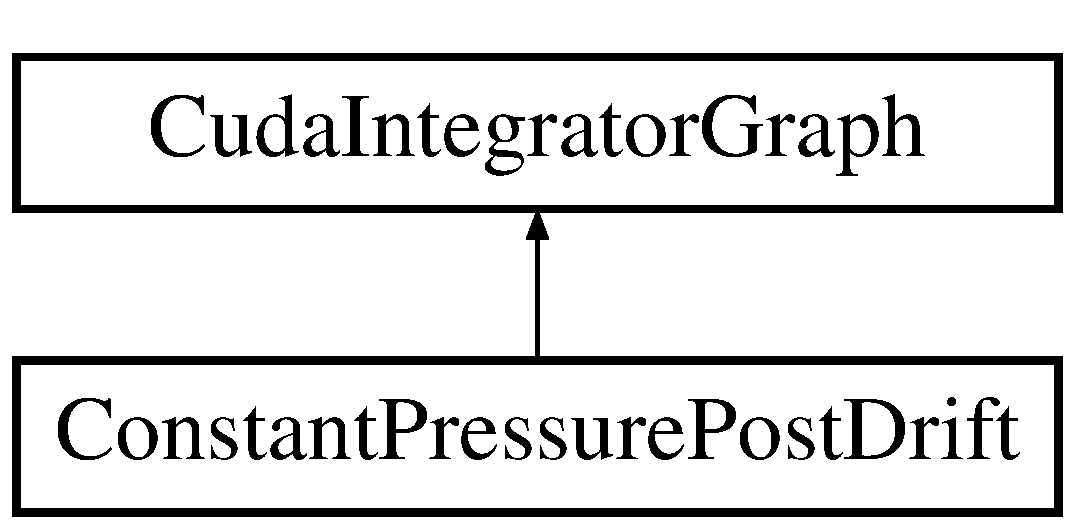
\includegraphics[height=2.000000cm]{classConstantPressurePostDrift}
\end{center}
\end{figure}
\subsection*{Public Member Functions}
\begin{DoxyCompactItemize}
\item 
\hyperlink{classConstantPressurePostDrift_ac04e5c4bcbd6f48169085138a157c2e8}{Constant\+Pressure\+Post\+Drift} (const double4 $\ast$\+\_\+\+\_\+restrict\+\_\+\+\_\+ relative\+\_\+xyzq, const double4 $\ast$\+\_\+\+\_\+restrict\+\_\+\+\_\+ relative\+\_\+vel\+\_\+mass, const \hyperlink{structComID__t}{Com\+I\+D\+\_\+t} $\ast$\+\_\+\+\_\+restrict\+\_\+\+\_\+ com\+\_\+ids, const double4 $\ast$\+\_\+\+\_\+restrict\+\_\+\+\_\+ com\+\_\+momentum\+\_\+invmass, double4 $\ast$\+\_\+\+\_\+restrict\+\_\+\+\_\+ absolute\+\_\+xyzq, double4 $\ast$\+\_\+\+\_\+restrict\+\_\+\+\_\+ absolute\+\_\+vel\+\_\+mass, const int $\ast$sorted\+\_\+atomids, int num\+Groups)
\begin{DoxyCompactList}\small\item\em Create a graph that gets absolute coords back from relative coords. \end{DoxyCompactList}\end{DoxyCompactItemize}
\subsection*{Additional Inherited Members}


\subsection{Detailed Description}
Create a graph that gets absolute coords back from relative coords. 



\subsection{Constructor \& Destructor Documentation}
\hypertarget{classConstantPressurePostDrift_ac04e5c4bcbd6f48169085138a157c2e8}{}\label{classConstantPressurePostDrift_ac04e5c4bcbd6f48169085138a157c2e8} 
\index{Constant\+Pressure\+Post\+Drift@{Constant\+Pressure\+Post\+Drift}!Constant\+Pressure\+Post\+Drift@{Constant\+Pressure\+Post\+Drift}}
\index{Constant\+Pressure\+Post\+Drift@{Constant\+Pressure\+Post\+Drift}!Constant\+Pressure\+Post\+Drift@{Constant\+Pressure\+Post\+Drift}}
\subsubsection{\texorpdfstring{Constant\+Pressure\+Post\+Drift()}{ConstantPressurePostDrift()}}
{\footnotesize\ttfamily Constant\+Pressure\+Post\+Drift\+::\+Constant\+Pressure\+Post\+Drift (\begin{DoxyParamCaption}\item[{const double4 $\ast$\+\_\+\+\_\+restrict\+\_\+\+\_\+}]{relative\+\_\+xyzq,  }\item[{const double4 $\ast$\+\_\+\+\_\+restrict\+\_\+\+\_\+}]{relative\+\_\+vel\+\_\+mass,  }\item[{const \hyperlink{structComID__t}{Com\+I\+D\+\_\+t} $\ast$\+\_\+\+\_\+restrict\+\_\+\+\_\+}]{com\+\_\+ids,  }\item[{const double4 $\ast$\+\_\+\+\_\+restrict\+\_\+\+\_\+}]{com\+\_\+momentum\+\_\+invmass,  }\item[{double4 $\ast$\+\_\+\+\_\+restrict\+\_\+\+\_\+}]{absolute\+\_\+xyzq,  }\item[{double4 $\ast$\+\_\+\+\_\+restrict\+\_\+\+\_\+}]{absolute\+\_\+vel\+\_\+mass,  }\item[{const int $\ast$}]{sorted\+\_\+atomids,  }\item[{int}]{num\+Groups }\end{DoxyParamCaption})}



Create a graph that gets absolute coords back from relative coords. 


\begin{DoxyParams}{Parameters}
{\em relative\+\_\+xyzq} & The device pointer to the array of atom positions relative to the center of mass of their pressure group. \\
\hline
{\em relative\+\_\+vel\+\_\+mass} & The device pointer to the array of relative velocity and mass of every atom. \\
\hline
{\em com\+\_\+ids} & The device pointer to the array of the position of the center of mass of each pressure group, and the atoms that are in the group. \\
\hline
{\em com\+\_\+momentum\+\_\+invmass} & The device pointer to the array of the group net momentums and inverse masses. \\
\hline
{\em absolute\+\_\+xyzq} & The device pointer to the array of absolute atom positions. \\
\hline
{\em absolute\+\_\+vel\+\_\+mass} & The device pointer to the array of absolute velocity and mass of every atom. \\
\hline
{\em sorted\+\_\+atomids} & Array of all atom ids sorted by pressure group. \\
\hline
{\em num\+Groups} & number of groups. \\
\hline
\end{DoxyParams}


The documentation for this class was generated from the following file\+:\begin{DoxyCompactItemize}
\item 
/u/samar/\+Documents/git/chcuda/include/\hyperlink{ConstantPressurePostDrift_8h}{Constant\+Pressure\+Post\+Drift.\+h}\end{DoxyCompactItemize}

\hypertarget{classConstantPressurePrepareDrift}{}\section{Constant\+Pressure\+Prepare\+Drift Class Reference}
\label{classConstantPressurePrepareDrift}\index{Constant\+Pressure\+Prepare\+Drift@{Constant\+Pressure\+Prepare\+Drift}}


Create a graph that calculates the net momentums, center of masses(\+C\+O\+M), relative coordinates to the C\+O\+Ms, internal momentums, and kinetic energies from the C\+OM motion, and kinetic energies from the internal motions.  




{\ttfamily \#include $<$Constant\+Pressure\+Prepare\+Drift.\+h$>$}

Inheritance diagram for Constant\+Pressure\+Prepare\+Drift\+:\begin{figure}[H]
\begin{center}
\leavevmode
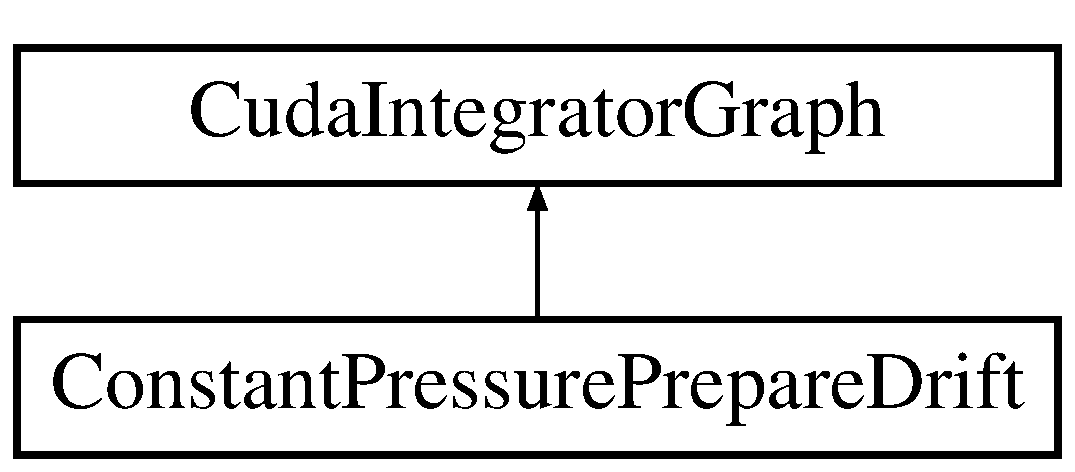
\includegraphics[height=2.000000cm]{classConstantPressurePrepareDrift}
\end{center}
\end{figure}
\subsection*{Public Member Functions}
\begin{DoxyCompactItemize}
\item 
\hyperlink{classConstantPressurePrepareDrift_acdf4bbe89bee70df889d745f1c8cf08c}{Constant\+Pressure\+Prepare\+Drift} (const double4 $\ast$\+\_\+\+\_\+restrict\+\_\+\+\_\+ absolute\+\_\+vel\+\_\+mass, const double4 $\ast$\+\_\+\+\_\+restrict\+\_\+\+\_\+ absolute\+\_\+xyzq, double4 $\ast$\+\_\+\+\_\+restrict\+\_\+\+\_\+ relative\+\_\+xyzq, double4 $\ast$\+\_\+\+\_\+restrict\+\_\+\+\_\+ relative\+\_\+vel\+\_\+mass, \hyperlink{structComID__t}{Com\+I\+D\+\_\+t} $\ast$\+\_\+\+\_\+restrict\+\_\+\+\_\+ com\+\_\+ids, double4 $\ast$\+\_\+\+\_\+restrict\+\_\+\+\_\+ com\+\_\+momentum\+\_\+invmass, double3 $\ast$\+\_\+\+\_\+restrict\+\_\+\+\_\+ com\+\_\+kinetic\+\_\+energy, double $\ast$\+\_\+\+\_\+restrict\+\_\+\+\_\+ total\+\_\+kinetic\+\_\+energy, const int $\ast$sorted\+\_\+atomids, int num\+Atoms, int num\+Groups)
\begin{DoxyCompactList}\small\item\em Create a graph that calculate the net momentums, center of masses(\+C\+O\+M), relative coordinates to the C\+O\+Ms, internal momentums, and kinetic energies from the C\+OM motion, and kinetic energies from the internal motions. \end{DoxyCompactList}\item 
\hyperlink{classConstantPressurePrepareDrift_a0df027b22f65f8ee39387d41e612120b}{$\sim$\+Constant\+Pressure\+Prepare\+Drift} ()
\begin{DoxyCompactList}\small\item\em Destroy the graph, its nodes, and free internal memory. \end{DoxyCompactList}\end{DoxyCompactItemize}
\subsection*{Additional Inherited Members}


\subsection{Detailed Description}
Create a graph that calculates the net momentums, center of masses(\+C\+O\+M), relative coordinates to the C\+O\+Ms, internal momentums, and kinetic energies from the C\+OM motion, and kinetic energies from the internal motions. 



\subsection{Constructor \& Destructor Documentation}
\hypertarget{classConstantPressurePrepareDrift_acdf4bbe89bee70df889d745f1c8cf08c}{}\label{classConstantPressurePrepareDrift_acdf4bbe89bee70df889d745f1c8cf08c} 
\index{Constant\+Pressure\+Prepare\+Drift@{Constant\+Pressure\+Prepare\+Drift}!Constant\+Pressure\+Prepare\+Drift@{Constant\+Pressure\+Prepare\+Drift}}
\index{Constant\+Pressure\+Prepare\+Drift@{Constant\+Pressure\+Prepare\+Drift}!Constant\+Pressure\+Prepare\+Drift@{Constant\+Pressure\+Prepare\+Drift}}
\subsubsection{\texorpdfstring{Constant\+Pressure\+Prepare\+Drift()}{ConstantPressurePrepareDrift()}}
{\footnotesize\ttfamily Constant\+Pressure\+Prepare\+Drift\+::\+Constant\+Pressure\+Prepare\+Drift (\begin{DoxyParamCaption}\item[{const double4 $\ast$\+\_\+\+\_\+restrict\+\_\+\+\_\+}]{absolute\+\_\+vel\+\_\+mass,  }\item[{const double4 $\ast$\+\_\+\+\_\+restrict\+\_\+\+\_\+}]{absolute\+\_\+xyzq,  }\item[{double4 $\ast$\+\_\+\+\_\+restrict\+\_\+\+\_\+}]{relative\+\_\+xyzq,  }\item[{double4 $\ast$\+\_\+\+\_\+restrict\+\_\+\+\_\+}]{relative\+\_\+vel\+\_\+mass,  }\item[{\hyperlink{structComID__t}{Com\+I\+D\+\_\+t} $\ast$\+\_\+\+\_\+restrict\+\_\+\+\_\+}]{com\+\_\+ids,  }\item[{double4 $\ast$\+\_\+\+\_\+restrict\+\_\+\+\_\+}]{com\+\_\+momentum\+\_\+invmass,  }\item[{double3 $\ast$\+\_\+\+\_\+restrict\+\_\+\+\_\+}]{com\+\_\+kinetic\+\_\+energy,  }\item[{double $\ast$\+\_\+\+\_\+restrict\+\_\+\+\_\+}]{total\+\_\+kinetic\+\_\+energy,  }\item[{const int $\ast$}]{sorted\+\_\+atomids,  }\item[{int}]{num\+Atoms,  }\item[{int}]{num\+Groups }\end{DoxyParamCaption})}



Create a graph that calculate the net momentums, center of masses(\+C\+O\+M), relative coordinates to the C\+O\+Ms, internal momentums, and kinetic energies from the C\+OM motion, and kinetic energies from the internal motions. 

All units are SI compatible. 
\begin{DoxyParams}{Parameters}
{\em absolute\+\_\+vel\+\_\+mass} & The device pointer to the array of absolute velocity and mass of every atom. \\
\hline
{\em absolute\+\_\+xyzq} & The device pointer to the array of absolute atom positions. \\
\hline
{\em relative\+\_\+xyzq} & The device pointer to the array of atom positions relative to the center of mass of their pressure group. \\
\hline
{\em relative\+\_\+vel\+\_\+mass} & The device pointer to the array of relative velocity and mass of every atom. \\
\hline
{\em com\+\_\+ids} & The device pointer to the array of the position of the center of mass of each pressure group, and the atoms that are in the group. \\
\hline
{\em com\+\_\+momentum\+\_\+invmass} & The device pointer to the array of the group net momentums and inverse masses. \\
\hline
{\em com\+\_\+kinetic\+\_\+energy} & The xx,yy, and zz components of the groups center of mass kinetic energy. \\
\hline
{\em total\+\_\+kinetic\+\_\+energy} & The total kinetic energy, used for the thermostat piston. \\
\hline
{\em sorted\+\_\+atomids} & Array of all atom ids sorted by pressure group. \\
\hline
{\em num\+Atoms} & number of atoms. \\
\hline
{\em num\+Groups} & number of groups. \\
\hline
\end{DoxyParams}
\hypertarget{classConstantPressurePrepareDrift_a0df027b22f65f8ee39387d41e612120b}{}\label{classConstantPressurePrepareDrift_a0df027b22f65f8ee39387d41e612120b} 
\index{Constant\+Pressure\+Prepare\+Drift@{Constant\+Pressure\+Prepare\+Drift}!````~Constant\+Pressure\+Prepare\+Drift@{$\sim$\+Constant\+Pressure\+Prepare\+Drift}}
\index{````~Constant\+Pressure\+Prepare\+Drift@{$\sim$\+Constant\+Pressure\+Prepare\+Drift}!Constant\+Pressure\+Prepare\+Drift@{Constant\+Pressure\+Prepare\+Drift}}
\subsubsection{\texorpdfstring{$\sim$\+Constant\+Pressure\+Prepare\+Drift()}{~ConstantPressurePrepareDrift()}}
{\footnotesize\ttfamily Constant\+Pressure\+Prepare\+Drift\+::$\sim$\+Constant\+Pressure\+Prepare\+Drift (\begin{DoxyParamCaption}{ }\end{DoxyParamCaption})}



Destroy the graph, its nodes, and free internal memory. 



The documentation for this class was generated from the following file\+:\begin{DoxyCompactItemize}
\item 
/u/samar/\+Documents/git/chcuda/include/\hyperlink{ConstantPressurePrepareDrift_8h}{Constant\+Pressure\+Prepare\+Drift.\+h}\end{DoxyCompactItemize}

\hypertarget{classCudaBlock}{}\section{Cuda\+Block Class Reference}
\label{classCudaBlock}\index{Cuda\+Block@{Cuda\+Block}}
\subsection*{Public Member Functions}
\begin{DoxyCompactItemize}
\item 
\hypertarget{classCudaBlock_a6131c6f8ed1abc5ba8fa4a2a2ca055d9}{}\label{classCudaBlock_a6131c6f8ed1abc5ba8fa4a2a2ca055d9} 
{\bfseries Cuda\+Block} (const int num\+Block, const int use\+\_\+softcore, const int use\+\_\+\+P\+M\+EL)
\item 
\hypertarget{classCudaBlock_a4781318d60ffec96616e3a4894b864a3}{}\label{classCudaBlock_a4781318d60ffec96616e3a4894b864a3} 
void {\bfseries set\+Block\+Type} (const int ncoord, const int $\ast$h\+\_\+block\+Type)
\item 
\hypertarget{classCudaBlock_aa83f8fc5096a4381314ac92183fbf636}{}\label{classCudaBlock_aa83f8fc5096a4381314ac92183fbf636} 
void {\bfseries set\+Block\+Param} (const float $\ast$h\+\_\+block\+Param\+Full)
\item 
\hypertarget{classCudaBlock_a0728de486ea9b102dca1bf822b1b2a6e}{}\label{classCudaBlock_a0728de486ea9b102dca1bf822b1b2a6e} 
void {\bfseries set\+Bixlam} (const float $\ast$h\+\_\+bixlam)
\item 
\hypertarget{classCudaBlock_a521b88d865583a6e5003dbcb8b9b66eb}{}\label{classCudaBlock_a521b88d865583a6e5003dbcb8b9b66eb} 
void {\bfseries set\+Site\+M\+LD} (const int $\ast$h\+\_\+site\+M\+LD)
\item 
\hypertarget{classCudaBlock_aff0a25b9d34200b1ddc0778cd09b9c93}{}\label{classCudaBlock_aff0a25b9d34200b1ddc0778cd09b9c93} 
int {\bfseries get\+Num\+Block} ()
\item 
\hypertarget{classCudaBlock_a393323b25d6ef181fbe368771b500c4a}{}\label{classCudaBlock_a393323b25d6ef181fbe368771b500c4a} 
int $\ast$ {\bfseries get\+Block\+Type} ()
\item 
\hypertarget{classCudaBlock_a63dbe00f85a571673f60184a37f6ce9e}{}\label{classCudaBlock_a63dbe00f85a571673f60184a37f6ce9e} 
float $\ast$ {\bfseries get\+Bixlam} ()
\item 
\hypertarget{classCudaBlock_a7ffeffc6327ad8423c575be514b884ae}{}\label{classCudaBlock_a7ffeffc6327ad8423c575be514b884ae} 
double $\ast$ {\bfseries get\+Biflam} ()
\item 
\hypertarget{classCudaBlock_a4786b3496e94c61c368c835b18759780}{}\label{classCudaBlock_a4786b3496e94c61c368c835b18759780} 
double $\ast$ {\bfseries get\+Biflam2} ()
\item 
\hypertarget{classCudaBlock_a084db6c66816cd67e7f1f4d5fdf45ed4}{}\label{classCudaBlock_a084db6c66816cd67e7f1f4d5fdf45ed4} 
void {\bfseries get\+Biflam} (double $\ast$h\+\_\+biflam, double $\ast$h\+\_\+biflam2)
\item 
\hypertarget{classCudaBlock_a10590b0590b77f035344c640910cc751}{}\label{classCudaBlock_a10590b0590b77f035344c640910cc751} 
void {\bfseries set\+Biflam} (double $\ast$h\+\_\+biflam, double $\ast$h\+\_\+biflam2)
\item 
\hypertarget{classCudaBlock_a3eb37141bc8dec2a147dc8510e855bb6}{}\label{classCudaBlock_a3eb37141bc8dec2a147dc8510e855bb6} 
float $\ast$ {\bfseries get\+Block\+Param} ()
\item 
\hypertarget{classCudaBlock_aed739a43cb9a49d6b090bc6b921b2a21}{}\label{classCudaBlock_aed739a43cb9a49d6b090bc6b921b2a21} 
float $\ast$ {\bfseries get\+Block\+Param\+Ex} ()
\item 
\hypertarget{classCudaBlock_a65af2f17a316387636944c6a53e2d74b}{}\label{classCudaBlock_a65af2f17a316387636944c6a53e2d74b} 
double $\ast$ {\bfseries get\+D\+Soft\+D\+Fscale} ()
\item 
\hypertarget{classCudaBlock_aa9c209c93a7c2c156a5ddf5caa23e6b9}{}\label{classCudaBlock_aa9c209c93a7c2c156a5ddf5caa23e6b9} 
float {\bfseries get\+Block\+Param\+Value} (const int k)
\item 
\hypertarget{classCudaBlock_ab66a4a3b414fe8ae0434e5e341c8ac92}{}\label{classCudaBlock_ab66a4a3b414fe8ae0434e5e341c8ac92} 
float {\bfseries get\+Block\+Param\+Ex\+Value} (const int k)
\item 
\hypertarget{classCudaBlock_a6e2e448f21d6580748af20feb52abeb8}{}\label{classCudaBlock_a6e2e448f21d6580748af20feb52abeb8} 
int $\ast$ {\bfseries get\+Site\+M\+LD} ()
\item 
\hypertarget{classCudaBlock_a99b0b2c2e791bcc8f480965eb428024e}{}\label{classCudaBlock_a99b0b2c2e791bcc8f480965eb428024e} 
int {\bfseries get\+Use\+Softcore} ()
\item 
\hypertarget{classCudaBlock_ad801d7ab49d72e118f0876f993d9866e}{}\label{classCudaBlock_ad801d7ab49d72e118f0876f993d9866e} 
int {\bfseries get\+Use\+P\+M\+EL} ()
\end{DoxyCompactItemize}


The documentation for this class was generated from the following file\+:\begin{DoxyCompactItemize}
\item 
/u/samar/\+Documents/git/chcuda/include/Cuda\+Block.\+h\end{DoxyCompactItemize}

\hypertarget{classCudaBondedForce}{}\section{Cuda\+Bonded\+Force$<$ AT, CT $>$ Class Template Reference}
\label{classCudaBondedForce}\index{Cuda\+Bonded\+Force$<$ A\+T, C\+T $>$@{Cuda\+Bonded\+Force$<$ A\+T, C\+T $>$}}
\subsection*{Public Member Functions}
\begin{DoxyCompactItemize}
\item 
\hypertarget{classCudaBondedForce_a187a309ec2cff80cde58651b6b7027f9}{}\label{classCudaBondedForce_a187a309ec2cff80cde58651b6b7027f9} 
{\bfseries Cuda\+Bonded\+Force} (\hyperlink{classCudaEnergyVirial}{Cuda\+Energy\+Virial} \&energy\+Virial, const char $\ast$name\+Bond, const char $\ast$name\+Ureyb, const char $\ast$name\+Angle, const char $\ast$name\+Dihe, const char $\ast$name\+Imdihe, const char $\ast$name\+Cmap)
\item 
\hypertarget{classCudaBondedForce_afbb956ecfefba60abf39ee5f918826e8}{}\label{classCudaBondedForce_afbb956ecfefba60abf39ee5f918826e8} 
void {\bfseries setup\+\_\+coef} (const int nbondcoef, const float2 $\ast$h\+\_\+bondcoef, const int nureybcoef, const float2 $\ast$h\+\_\+ureybcoef, const int nanglecoef, const float2 $\ast$h\+\_\+anglecoef, const int ndihecoef, const float4 $\ast$h\+\_\+dihecoef, const int nimdihecoef, const float4 $\ast$h\+\_\+imdihecoef, const int ncmapcoef, const float2 $\ast$h\+\_\+cmapcoef)
\item 
\hypertarget{classCudaBondedForce_a41719ddc963ea1ef2da1fc4e174c4b95}{}\label{classCudaBondedForce_a41719ddc963ea1ef2da1fc4e174c4b95} 
void {\bfseries setup\+\_\+list} (const int nbondlist, const \hyperlink{structbondlist__t}{bondlist\+\_\+t} $\ast$h\+\_\+bondlist, const int nureyblist, const \hyperlink{structbondlist__t}{bondlist\+\_\+t} $\ast$h\+\_\+ureyblist, const int nanglelist, const \hyperlink{structanglelist__t}{anglelist\+\_\+t} $\ast$h\+\_\+anglelist, const int ndihelist, const \hyperlink{structdihelist__t}{dihelist\+\_\+t} $\ast$h\+\_\+dihelist, const int nimdihelist, const \hyperlink{structdihelist__t}{dihelist\+\_\+t} $\ast$h\+\_\+imdihelist, const int ncmaplist, const \hyperlink{structcmaplist__t}{cmaplist\+\_\+t} $\ast$h\+\_\+cmaplist, cuda\+Stream\+\_\+t stream=0)
\item 
\hypertarget{classCudaBondedForce_a2cb00b3eb0621b031c69db4afdd35371}{}\label{classCudaBondedForce_a2cb00b3eb0621b031c69db4afdd35371} 
void {\bfseries setup\+\_\+list} (const float4 $\ast$xyzq, const CT boxx, const CT boxy, const CT boxz, const int $\ast$glo2loc\+\_\+ind, const int nbond\+\_\+tbl, const int $\ast$bond\+\_\+tbl, const \hyperlink{structbond__t}{bond\+\_\+t} $\ast$bond, const int nureyb\+\_\+tbl, const int $\ast$ureyb\+\_\+tbl, const \hyperlink{structbond__t}{bond\+\_\+t} $\ast$ureyb, const int nangle\+\_\+tbl, const int $\ast$angle\+\_\+tbl, const \hyperlink{structangle__t}{angle\+\_\+t} $\ast$angle, const int ndihe\+\_\+tbl, const int $\ast$dihe\+\_\+tbl, const \hyperlink{structdihe__t}{dihe\+\_\+t} $\ast$dihe, const int nimdihe\+\_\+tbl, const int $\ast$imdihe\+\_\+tbl, const \hyperlink{structdihe__t}{dihe\+\_\+t} $\ast$imdihe, const int ncmap\+\_\+tbl, const int $\ast$cmap\+\_\+tbl, const \hyperlink{structcmap__t}{cmap\+\_\+t} $\ast$cmap, cuda\+Stream\+\_\+t stream=0)
\item 
\hypertarget{classCudaBondedForce_a762489ffa9c804e654658a6f30b529dd}{}\label{classCudaBondedForce_a762489ffa9c804e654658a6f30b529dd} 
void {\bfseries calc\+\_\+force} (const float4 $\ast$xyzq, const CT boxx, const CT boxy, const CT boxz, const bool calc\+\_\+energy, const bool calc\+\_\+virial, const int stride, AT $\ast$force, const bool calc\+\_\+bond, const bool calc\+\_\+ureyb, const bool calc\+\_\+angle, const bool calc\+\_\+dihe, const bool calc\+\_\+imdihe, const bool calc\+\_\+cmap, cuda\+Stream\+\_\+t stream=0)
\item 
\hypertarget{classCudaBondedForce_a0829dcaac9739741280babcb491895d1}{}\label{classCudaBondedForce_a0829dcaac9739741280babcb491895d1} 
void {\bfseries print} ()
\end{DoxyCompactItemize}


The documentation for this class was generated from the following file\+:\begin{DoxyCompactItemize}
\item 
/u/samar/\+Documents/git/chcuda/include/Cuda\+Bonded\+Force.\+h\end{DoxyCompactItemize}

\hypertarget{classCudaContainer}{}\section{Cuda\+Container$<$ T $>$ Class Template Reference}
\label{classCudaContainer}\index{Cuda\+Container$<$ T $>$@{Cuda\+Container$<$ T $>$}}
\subsection*{Public Member Functions}
\begin{DoxyCompactItemize}
\item 
\hypertarget{classCudaContainer_a38277438880c3e1b2b44c13f5928ac6d}{}\label{classCudaContainer_a38277438880c3e1b2b44c13f5928ac6d} 
size\+\_\+t {\bfseries size} () const
\item 
\hypertarget{classCudaContainer_a708fda937e504d25ddfe1081ac2d96da}{}\label{classCudaContainer_a708fda937e504d25ddfe1081ac2d96da} 
void {\bfseries allocate} (size\+\_\+t size)
\item 
\hypertarget{classCudaContainer_ae775cb3d0fd2929ff7f608bf19efd493}{}\label{classCudaContainer_ae775cb3d0fd2929ff7f608bf19efd493} 
void {\bfseries set\+Host\+Array} (const std\+::vector$<$ T $>$ \&array)
\item 
\hypertarget{classCudaContainer_a5a03f48d9414f2900996f77503c78ae8}{}\label{classCudaContainer_a5a03f48d9414f2900996f77503c78ae8} 
const std\+::vector$<$ T $>$ \& {\bfseries get\+Host\+Array} ()
\item 
\hypertarget{classCudaContainer_a6137c9e3b52fbe34b298b86de2e875e0}{}\label{classCudaContainer_a6137c9e3b52fbe34b298b86de2e875e0} 
void {\bfseries transfer\+To\+Device} ()
\item 
\hypertarget{classCudaContainer_a1bbe7a7a89334d96338f6879785628bb}{}\label{classCudaContainer_a1bbe7a7a89334d96338f6879785628bb} 
void {\bfseries transfer\+From\+Device} ()
\item 
\hypertarget{classCudaContainer_ac57550f6bc543449a98705106552efdf}{}\label{classCudaContainer_ac57550f6bc543449a98705106552efdf} 
void {\bfseries print\+Device} ()
\item 
\hypertarget{classCudaContainer_a1900957efd8ecf717d181e9f3b29c911}{}\label{classCudaContainer_a1900957efd8ecf717d181e9f3b29c911} 
void {\bfseries set} (const std\+::vector$<$ T $>$ \&inp\+Vec)
\end{DoxyCompactItemize}


The documentation for this class was generated from the following file\+:\begin{DoxyCompactItemize}
\item 
/u/samar/\+Documents/git/chcuda/include/Cuda\+Container.\+h\end{DoxyCompactItemize}

\hypertarget{classCudaDomdecRecip}{}\section{Cuda\+Domdec\+Recip Class Reference}
\label{classCudaDomdecRecip}\index{Cuda\+Domdec\+Recip@{Cuda\+Domdec\+Recip}}
Inheritance diagram for Cuda\+Domdec\+Recip\+:\begin{figure}[H]
\begin{center}
\leavevmode
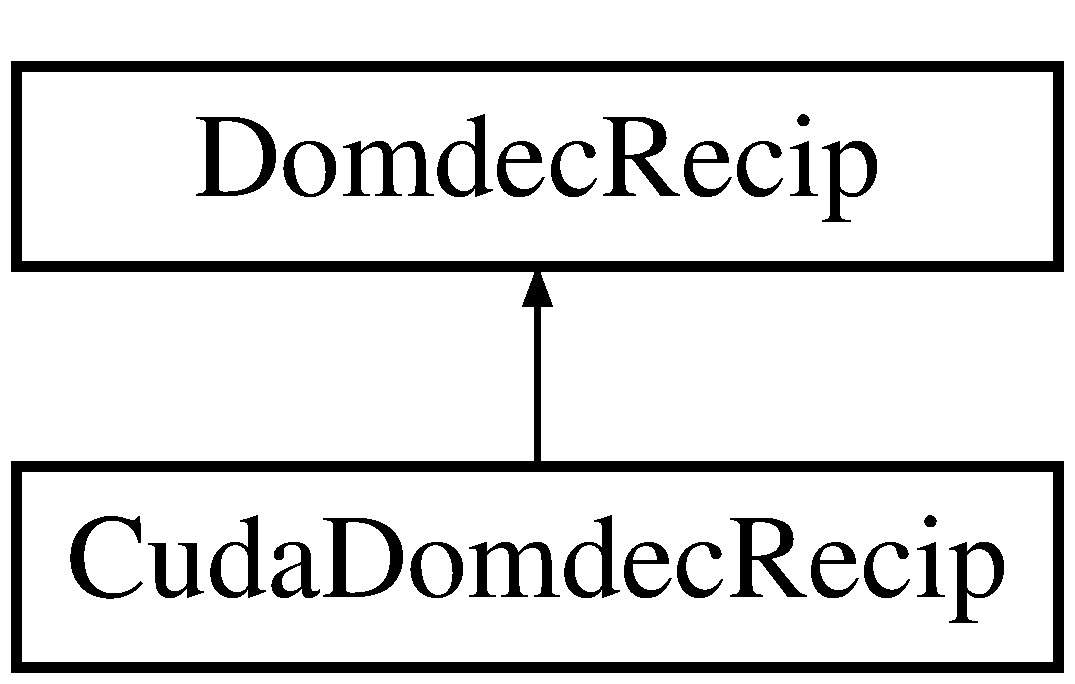
\includegraphics[height=2.000000cm]{classCudaDomdecRecip}
\end{center}
\end{figure}
\subsection*{Public Member Functions}
\begin{DoxyCompactItemize}
\item 
\hypertarget{classCudaDomdecRecip_adaa2c67c3f03b4088290625e8bd9f74e}{}\label{classCudaDomdecRecip_adaa2c67c3f03b4088290625e8bd9f74e} 
{\bfseries Cuda\+Domdec\+Recip} (\hyperlink{classCudaEnergyVirial}{Cuda\+Energy\+Virial} \&energy\+Virial)
\item 
\hypertarget{classCudaDomdecRecip_a24e6d5cb0a64a025aeb1fdee6a821a75}{}\label{classCudaDomdecRecip_a24e6d5cb0a64a025aeb1fdee6a821a75} 
{\bfseries Cuda\+Domdec\+Recip} (const int nfftx, const int nffty, const int nfftz, const int order, const double kappa, \hyperlink{classCudaEnergyVirial}{Cuda\+Energy\+Virial} \&energy\+Virial, const char $\ast$name\+Recip, const char $\ast$name\+Self)
\item 
\hypertarget{classCudaDomdecRecip_a96ef44bed53448a42f5a9157a865741a}{}\label{classCudaDomdecRecip_a96ef44bed53448a42f5a9157a865741a} 
void {\bfseries set\+Parameters} (int nfft1, int nfft2, int nfft3, int sp, float k)
\item 
\hypertarget{classCudaDomdecRecip_a1cbec44daee4593e45008969ac6bc9a8}{}\label{classCudaDomdecRecip_a1cbec44daee4593e45008969ac6bc9a8} 
void {\bfseries set\+\_\+stream} (cuda\+Stream\+\_\+t stream)
\item 
\hypertarget{classCudaDomdecRecip_a6d0eac7f0a171854b40d2803e16c2283}{}\label{classCudaDomdecRecip_a6d0eac7f0a171854b40d2803e16c2283} 
void {\bfseries calc} (const double inv\+\_\+boxx, const double inv\+\_\+boxy, const double inv\+\_\+boxz, const float4 $\ast$coord, const int ncoord, const bool calc\+\_\+energy, const bool calc\+\_\+virial, \hyperlink{classForce}{Force}$<$ long long int $>$ \&force)
\item 
\hypertarget{classCudaDomdecRecip_a3d21fc32f495b991c3cd24cd5c133215}{}\label{classCudaDomdecRecip_a3d21fc32f495b991c3cd24cd5c133215} 
void {\bfseries calc} (const double inv\+\_\+boxx, const double inv\+\_\+boxy, const double inv\+\_\+boxz, const float4 $\ast$coord, const int ncoord, const bool calc\+\_\+energy, const bool calc\+\_\+virial, \hyperlink{classForce}{Force}$<$ float $>$ \&force)
\item 
\hypertarget{classCudaDomdecRecip_aaaf9f7a2192c4a6a7293a7ed75071bc8}{}\label{classCudaDomdecRecip_aaaf9f7a2192c4a6a7293a7ed75071bc8} 
void {\bfseries calc} (const double inv\+\_\+boxx, const double inv\+\_\+boxy, const double inv\+\_\+boxz, const float4 $\ast$coord, const int ncoord, const bool calc\+\_\+energy, const bool calc\+\_\+virial, float3 $\ast$force)
\item 
\hypertarget{classCudaDomdecRecip_a939aa363b653daa73d94d2bcfa015afe}{}\label{classCudaDomdecRecip_a939aa363b653daa73d94d2bcfa015afe} 
void {\bfseries calc\+\_\+block} (const double inv\+\_\+boxx, const double inv\+\_\+boxy, const double inv\+\_\+boxz, const float4 $\ast$coord, const int ncoord, const float $\ast$bixlam, const bool calc\+\_\+energy, const bool calc\+\_\+virial, \hyperlink{classForce}{Force}$<$ long long int $>$ \&force, double $\ast$biflam, const int $\ast$block\+Indexes)
\item 
\hypertarget{classCudaDomdecRecip_a9a81a01ef5d6385329c13423412c6e0a}{}\label{classCudaDomdecRecip_a9a81a01ef5d6385329c13423412c6e0a} 
void {\bfseries calc\+\_\+block} (const double inv\+\_\+boxx, const double inv\+\_\+boxy, const double inv\+\_\+boxz, const float4 $\ast$coord, const int ncoord, const float $\ast$bixlam, const bool calc\+\_\+energy, const bool calc\+\_\+virial, \hyperlink{classForce}{Force}$<$ float $>$ \&force, double $\ast$biflam, const int $\ast$block\+Indexes)
\item 
\hypertarget{classCudaDomdecRecip_a09d3f40535886d3c153a332e9c669d81}{}\label{classCudaDomdecRecip_a09d3f40535886d3c153a332e9c669d81} 
void {\bfseries calc\+\_\+block} (const double inv\+\_\+boxx, const double inv\+\_\+boxy, const double inv\+\_\+boxz, const float4 $\ast$coord, const int ncoord, const float $\ast$bixlam, const bool calc\+\_\+energy, const bool calc\+\_\+virial, float3 $\ast$force, double $\ast$biflam, const int $\ast$block\+Indexes)
\item 
\hypertarget{classCudaDomdecRecip_a0a695ab739249c06fa47033638efae3b}{}\label{classCudaDomdecRecip_a0a695ab739249c06fa47033638efae3b} 
int {\bfseries get\+F\+F\+TX} ()
\end{DoxyCompactItemize}
\subsection*{Additional Inherited Members}


The documentation for this class was generated from the following file\+:\begin{DoxyCompactItemize}
\item 
/u/samar/\+Documents/git/chcuda/include/Cuda\+Domdec\+Recip.\+h\end{DoxyCompactItemize}

\hypertarget{classCudaEnergyVirial}{}\section{Cuda\+Energy\+Virial Class Reference}
\label{classCudaEnergyVirial}\index{Cuda\+Energy\+Virial@{Cuda\+Energy\+Virial}}
Inheritance diagram for Cuda\+Energy\+Virial\+:\begin{figure}[H]
\begin{center}
\leavevmode
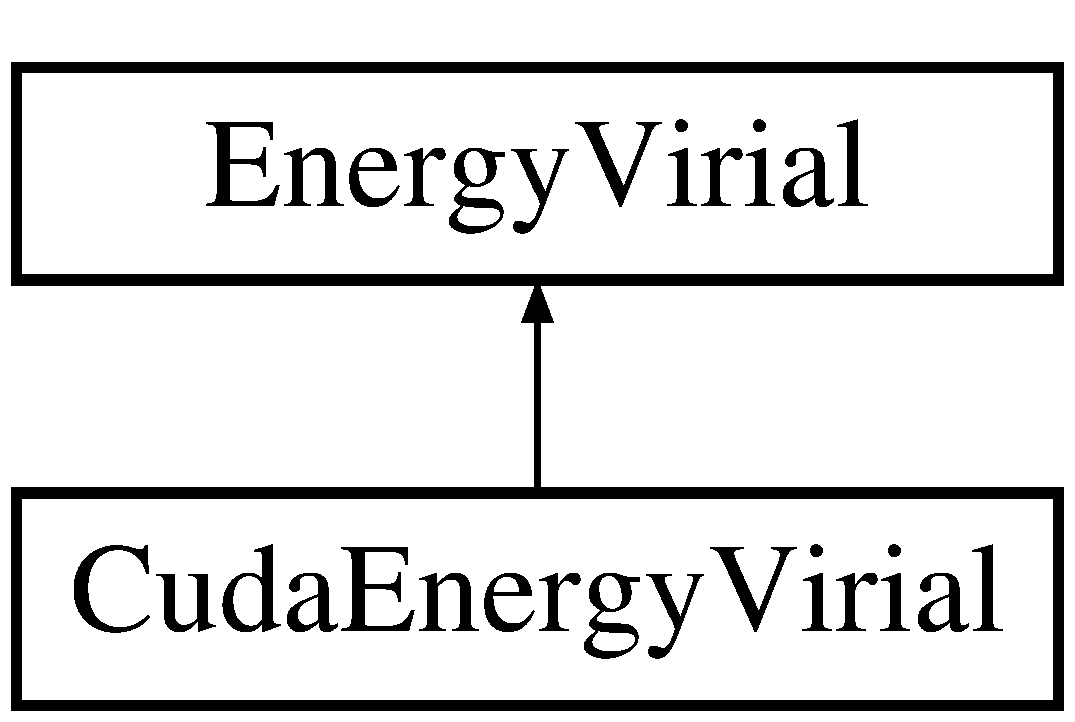
\includegraphics[height=2.000000cm]{classCudaEnergyVirial}
\end{center}
\end{figure}
\subsection*{Public Member Functions}
\begin{DoxyCompactItemize}
\item 
\hypertarget{classCudaEnergyVirial_abd7c7541d63e6070b090d911cfb27eb0}{}\label{classCudaEnergyVirial_abd7c7541d63e6070b090d911cfb27eb0} 
void {\bfseries clear} (cuda\+Stream\+\_\+t stream=0)
\item 
\hypertarget{classCudaEnergyVirial_a16fb1cc80eb715665e18f0d68dd27f79}{}\label{classCudaEnergyVirial_a16fb1cc80eb715665e18f0d68dd27f79} 
void {\bfseries clear\+Energy} (cuda\+Stream\+\_\+t stream=0)
\item 
\hypertarget{classCudaEnergyVirial_aa25dbdc2b516c3edad08972c0aed6c62}{}\label{classCudaEnergyVirial_aa25dbdc2b516c3edad08972c0aed6c62} 
void {\bfseries clear\+Eterm\+Device} (std\+::string \&name\+Eterm, cuda\+Stream\+\_\+t stream=0)
\item 
\hypertarget{classCudaEnergyVirial_adaaf288d88c47f0fa9edb344dec51a6f}{}\label{classCudaEnergyVirial_adaaf288d88c47f0fa9edb344dec51a6f} 
void {\bfseries clear\+Virial} (cuda\+Stream\+\_\+t stream=0)
\item 
\hypertarget{classCudaEnergyVirial_a0b480c2fcd79d10e60e78630ccda151c}{}\label{classCudaEnergyVirial_a0b480c2fcd79d10e60e78630ccda151c} 
void {\bfseries calc\+Virial} (const int ncoord, const float4 $\ast$xyzq, const double boxx, const double boxy, const double boxz, const int stride, const double $\ast$force, cuda\+Stream\+\_\+t stream=0)
\item 
\hypertarget{classCudaEnergyVirial_aec2ddf4b9c9b48d293076292fc673243}{}\label{classCudaEnergyVirial_aec2ddf4b9c9b48d293076292fc673243} 
void {\bfseries copy\+To\+Host} (cuda\+Stream\+\_\+t stream=0)
\item 
\hypertarget{classCudaEnergyVirial_ab269fa6df3d5ad84463614447b32748f}{}\label{classCudaEnergyVirial_ab269fa6df3d5ad84463614447b32748f} 
\hyperlink{structVirial__t}{Virial\+\_\+t} $\ast$ {\bfseries get\+Virial\+Pointer} ()
\item 
\hypertarget{classCudaEnergyVirial_aed8dcbf3e902dc8562c829798406c568}{}\label{classCudaEnergyVirial_aed8dcbf3e902dc8562c829798406c568} 
double $\ast$ {\bfseries get\+Energy\+Pointer} (std\+::string \&name)
\item 
\hypertarget{classCudaEnergyVirial_aa0c31fb5443de9daae00b05a5f7a73d5}{}\label{classCudaEnergyVirial_aa0c31fb5443de9daae00b05a5f7a73d5} 
double {\bfseries get\+Energy} (std\+::string \&name)
\item 
\hypertarget{classCudaEnergyVirial_ab834443e15f701d1f8613f738b21ed6e}{}\label{classCudaEnergyVirial_ab834443e15f701d1f8613f738b21ed6e} 
double {\bfseries get\+Energy} (const char $\ast$name)
\item 
\hypertarget{classCudaEnergyVirial_a7a18adcc1edd0e33b3586e4098810e8c}{}\label{classCudaEnergyVirial_a7a18adcc1edd0e33b3586e4098810e8c} 
void {\bfseries get\+Virial} (double $\ast$virmat)
\item 
\hypertarget{classCudaEnergyVirial_a101478267c320a2c6b65b2f8a2079440}{}\label{classCudaEnergyVirial_a101478267c320a2c6b65b2f8a2079440} 
void {\bfseries get\+Sforce} (double $\ast$sforce)
\end{DoxyCompactItemize}
\subsection*{Additional Inherited Members}


The documentation for this class was generated from the following file\+:\begin{DoxyCompactItemize}
\item 
/u/samar/\+Documents/git/chcuda/include/Cuda\+Energy\+Virial.\+h\end{DoxyCompactItemize}

\hypertarget{classCudaIntegrator}{}\section{Cuda\+Integrator Class Reference}
\label{classCudaIntegrator}\index{Cuda\+Integrator@{Cuda\+Integrator}}
Inheritance diagram for Cuda\+Integrator\+:\begin{figure}[H]
\begin{center}
\leavevmode
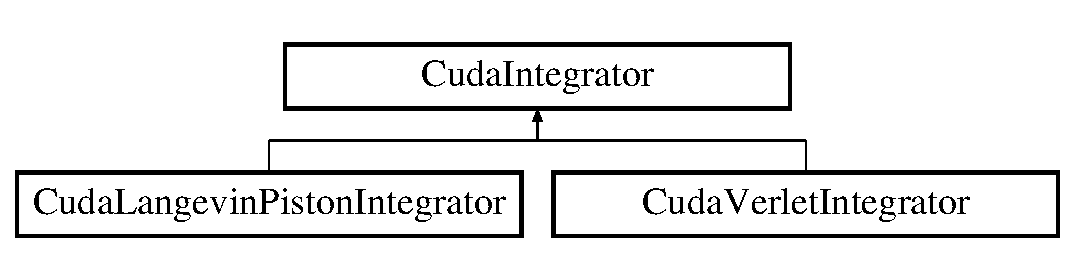
\includegraphics[height=2.000000cm]{classCudaIntegrator}
\end{center}
\end{figure}
\subsection*{Public Member Functions}
\begin{DoxyCompactItemize}
\item 
\hypertarget{classCudaIntegrator_ab7621d9a4ab2670adae56bc60cde75d0}{}\label{classCudaIntegrator_ab7621d9a4ab2670adae56bc60cde75d0} 
{\bfseries Cuda\+Integrator} (double time\+Step)
\item 
\hypertarget{classCudaIntegrator_af8f36da06802610a606bc1ac2ce978d7}{}\label{classCudaIntegrator_af8f36da06802610a606bc1ac2ce978d7} 
double {\bfseries get\+Time\+Step} () const
\item 
\hypertarget{classCudaIntegrator_a97a3ee2ca6b5501813eab968e65af0e2}{}\label{classCudaIntegrator_a97a3ee2ca6b5501813eab968e65af0e2} 
void {\bfseries set\+Time\+Step} (const double dt)
\item 
\hypertarget{classCudaIntegrator_ac74c2487586d922c28bd7b82a21c22af}{}\label{classCudaIntegrator_ac74c2487586d922c28bd7b82a21c22af} 
void {\bfseries set\+Simulation\+Context} (\hyperlink{classCudaSimulationContext}{Cuda\+Simulation\+Context} $\ast$csc)
\item 
\hypertarget{classCudaIntegrator_a4621ef339356331a782a00e392293364}{}\label{classCudaIntegrator_a4621ef339356331a782a00e392293364} 
void {\bfseries initialize\+Old\+New\+Coords} (int num\+Atoms)
\end{DoxyCompactItemize}
\subsection*{Protected Attributes}
\begin{DoxyCompactItemize}
\item 
\hypertarget{classCudaIntegrator_a8099cf8ab53d97b86623f0dd69c21510}{}\label{classCudaIntegrator_a8099cf8ab53d97b86623f0dd69c21510} 
double {\bfseries time\+Step}
\item 
\hypertarget{classCudaIntegrator_ae67486fba39d17c10f8274f4f41ef86a}{}\label{classCudaIntegrator_ae67486fba39d17c10f8274f4f41ef86a} 
\hyperlink{classCudaSimulationContext}{Cuda\+Simulation\+Context} $\ast$ {\bfseries simulation\+Context}
\item 
\hypertarget{classCudaIntegrator_ae792b058acda2cea2bed9938a75ba17f}{}\label{classCudaIntegrator_ae792b058acda2cea2bed9938a75ba17f} 
\hyperlink{classXYZQ}{X\+Y\+ZQ} $\ast$ {\bfseries old\+X\+Y\+ZQ}
\item 
\hypertarget{classCudaIntegrator_a15a43a80efa6fd81a1d7f922282c4c29}{}\label{classCudaIntegrator_a15a43a80efa6fd81a1d7f922282c4c29} 
\hyperlink{classXYZQ}{X\+Y\+ZQ} $\ast$ {\bfseries new\+X\+Y\+ZQ}
\end{DoxyCompactItemize}


The documentation for this class was generated from the following file\+:\begin{DoxyCompactItemize}
\item 
/u/samar/\+Documents/git/chcuda/include/Cuda\+Integrator.\+h\end{DoxyCompactItemize}

\hypertarget{classCudaIntegratorGraph}{}\section{Cuda\+Integrator\+Graph Class Reference}
\label{classCudaIntegratorGraph}\index{Cuda\+Integrator\+Graph@{Cuda\+Integrator\+Graph}}


Base class for other cuda integrator classes.  




{\ttfamily \#include $<$Cuda\+Integrator\+Graph.\+h$>$}

Inheritance diagram for Cuda\+Integrator\+Graph\+:\begin{figure}[H]
\begin{center}
\leavevmode
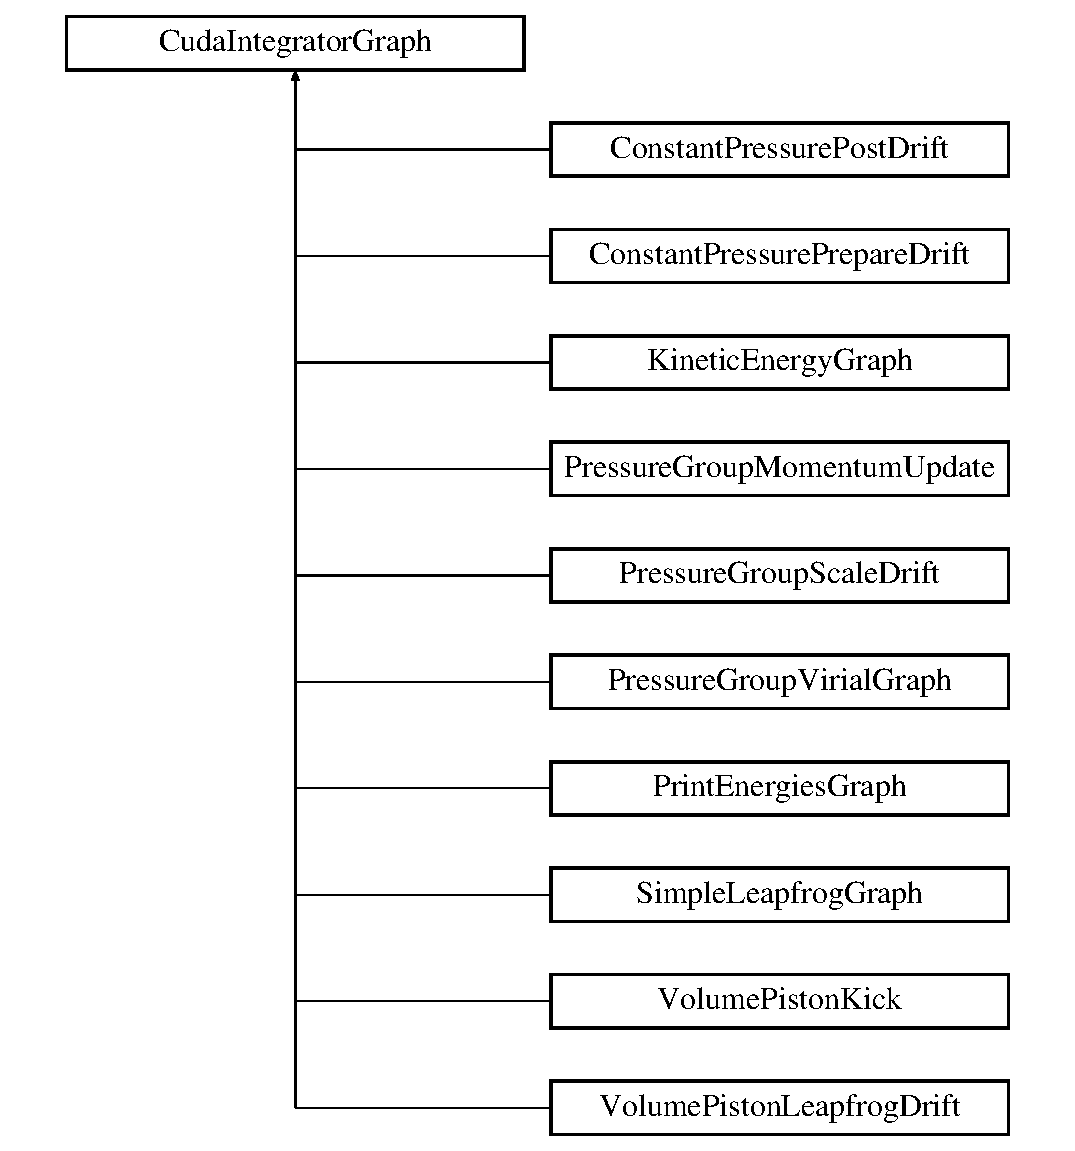
\includegraphics[height=11.000000cm]{classCudaIntegratorGraph}
\end{center}
\end{figure}
\subsection*{Public Member Functions}
\begin{DoxyCompactItemize}
\item 
\hypertarget{classCudaIntegratorGraph_ada9aeaf0aa6304abfcf095c72eaff25b}{}\label{classCudaIntegratorGraph_ada9aeaf0aa6304abfcf095c72eaff25b} 
\hyperlink{classCudaIntegratorGraph_ada9aeaf0aa6304abfcf095c72eaff25b}{Cuda\+Integrator\+Graph} ()
\begin{DoxyCompactList}\small\item\em Create a graph with one empty node. \end{DoxyCompactList}\item 
\hypertarget{classCudaIntegratorGraph_a32f852954891dc8af98a2b4b13885e1c}{}\label{classCudaIntegratorGraph_a32f852954891dc8af98a2b4b13885e1c} 
cuda\+Graph\+\_\+t \hyperlink{classCudaIntegratorGraph_a32f852954891dc8af98a2b4b13885e1c}{get\+Graph} ()
\begin{DoxyCompactList}\small\item\em Return the graph. \end{DoxyCompactList}\item 
\hypertarget{classCudaIntegratorGraph_a755fba1dde4ecb2e69b11ef279db9f0c}{}\label{classCudaIntegratorGraph_a755fba1dde4ecb2e69b11ef279db9f0c} 
\hyperlink{classCudaIntegratorGraph_a755fba1dde4ecb2e69b11ef279db9f0c}{$\sim$\+Cuda\+Integrator\+Graph} ()
\begin{DoxyCompactList}\small\item\em Destroy the graph and its nodes. \end{DoxyCompactList}\end{DoxyCompactItemize}
\subsection*{Protected Attributes}
\begin{DoxyCompactItemize}
\item 
\hypertarget{classCudaIntegratorGraph_a0811a0058f6b1bea2a9eef5392bddfba}{}\label{classCudaIntegratorGraph_a0811a0058f6b1bea2a9eef5392bddfba} 
cuda\+Graph\+\_\+t {\bfseries graph}
\end{DoxyCompactItemize}


\subsection{Detailed Description}
Base class for other cuda integrator classes. 



The documentation for this class was generated from the following file\+:\begin{DoxyCompactItemize}
\item 
/u/samar/\+Documents/git/chcuda/include/\hyperlink{CudaIntegratorGraph_8h}{Cuda\+Integrator\+Graph.\+h}\end{DoxyCompactItemize}

\hypertarget{classCudaLangevinPistonIntegrator}{}\section{Cuda\+Langevin\+Piston\+Integrator Class Reference}
\label{classCudaLangevinPistonIntegrator}\index{Cuda\+Langevin\+Piston\+Integrator@{Cuda\+Langevin\+Piston\+Integrator}}
Inheritance diagram for Cuda\+Langevin\+Piston\+Integrator\+:\begin{figure}[H]
\begin{center}
\leavevmode
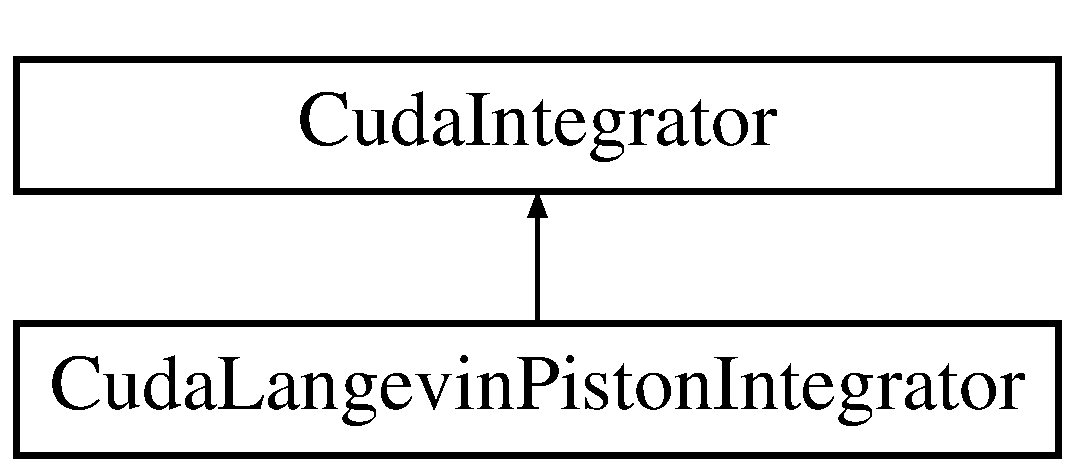
\includegraphics[height=2.000000cm]{classCudaLangevinPistonIntegrator}
\end{center}
\end{figure}
\subsection*{Public Member Functions}
\begin{DoxyCompactItemize}
\item 
\hypertarget{classCudaLangevinPistonIntegrator_a155720cf3dfca2b6f602d02af7b314e6}{}\label{classCudaLangevinPistonIntegrator_a155720cf3dfca2b6f602d02af7b314e6} 
{\bfseries Cuda\+Langevin\+Piston\+Integrator} (double time\+Step)
\item 
\hypertarget{classCudaLangevinPistonIntegrator_aa79fb4345b13e2a579e19e501bf46b1d}{}\label{classCudaLangevinPistonIntegrator_aa79fb4345b13e2a579e19e501bf46b1d} 
void {\bfseries initialize} ()
\item 
\hypertarget{classCudaLangevinPistonIntegrator_a3d7261a1661992bc0e24d599307d1489}{}\label{classCudaLangevinPistonIntegrator_a3d7261a1661992bc0e24d599307d1489} 
void {\bfseries propagate} (int n\+Steps)
\end{DoxyCompactItemize}
\subsection*{Additional Inherited Members}


The documentation for this class was generated from the following file\+:\begin{DoxyCompactItemize}
\item 
/u/samar/\+Documents/git/chcuda/include/Cuda\+Langevin\+Piston\+Integrator.\+h\end{DoxyCompactItemize}

\hypertarget{classCudaNeighborList}{}\section{Cuda\+Neighbor\+List$<$ tilesize $>$ Class Template Reference}
\label{classCudaNeighborList}\index{Cuda\+Neighbor\+List$<$ tilesize $>$@{Cuda\+Neighbor\+List$<$ tilesize $>$}}
\subsection*{Public Member Functions}
\begin{DoxyCompactItemize}
\item 
\hypertarget{classCudaNeighborList_a195cb796422518b661ac7d1c08fb14a2}{}\label{classCudaNeighborList_a195cb796422518b661ac7d1c08fb14a2} 
{\bfseries Cuda\+Neighbor\+List} (const \hyperlink{classCudaTopExcl}{Cuda\+Top\+Excl} \&top\+Excl, const int nx, const int ny, const int nz)
\item 
\hypertarget{classCudaNeighborList_a9c3f22487d9ccc310a7423d84e9761a1}{}\label{classCudaNeighborList_a9c3f22487d9ccc310a7423d84e9761a1} 
void {\bfseries register\+List} (std\+::vector$<$ int $>$ \&num\+Int\+Zone, std\+::vector$<$ std\+::vector$<$ int $>$ $>$ \&int\+Zones, const char $\ast$filename=N\+U\+LL)
\item 
\hypertarget{classCudaNeighborList_afa5fef8705b03909572827b528c90672}{}\label{classCudaNeighborList_afa5fef8705b03909572827b528c90672} 
void {\bfseries sort} (const int ind\+List, const int $\ast$zone\+\_\+patom, const float4 $\ast$xyzq, float4 $\ast$xyzq\+\_\+sorted, int $\ast$loc2glo, cuda\+Stream\+\_\+t stream=0)
\item 
\hypertarget{classCudaNeighborList_afe2e41c8aa957a87b2ecfb06e586a266}{}\label{classCudaNeighborList_afe2e41c8aa957a87b2ecfb06e586a266} 
void {\bfseries build} (const int ind\+List, const int $\ast$zone\+\_\+patom, const float boxx, const float boxy, const float boxz, const float rcut, const float4 $\ast$xyzq, const int $\ast$loc2glo, cuda\+Stream\+\_\+t stream=0)
\item 
\hypertarget{classCudaNeighborList_ad178c1accd50c60a1df81fbb9b81ec1f}{}\label{classCudaNeighborList_ad178c1accd50c60a1df81fbb9b81ec1f} 
int $\ast$ {\bfseries get\+\_\+glo2loc} ()
\item 
\hypertarget{classCudaNeighborList_a96b7d2f83fa52799f79b83df80f75e39}{}\label{classCudaNeighborList_a96b7d2f83fa52799f79b83df80f75e39} 
int $\ast$ {\bfseries get\+\_\+ind\+\_\+sorted} ()
\item 
\hypertarget{classCudaNeighborList_acf881a8245ab7e077122bda0ab57f9de}{}\label{classCudaNeighborList_acf881a8245ab7e077122bda0ab57f9de} 
int {\bfseries get\+Num\+List} ()
\item 
\hypertarget{classCudaNeighborList_a2158fc32438bb35d3b2170fb0ee36fed}{}\label{classCudaNeighborList_a2158fc32438bb35d3b2170fb0ee36fed} 
void {\bfseries set\+\_\+test} (bool test\+\_\+in)
\item 
\hypertarget{classCudaNeighborList_ac481b590ff46bd7bcf159c0655b9f080}{}\label{classCudaNeighborList_ac481b590ff46bd7bcf159c0655b9f080} 
\hyperlink{classCudaNeighborListBuild}{Cuda\+Neighbor\+List\+Build}$<$ tilesize $>$ \& {\bfseries get\+Builder} (const int ind\+List)
\item 
\hypertarget{classCudaNeighborList_a2b1c5d91c32e1628090998b9639320fa}{}\label{classCudaNeighborList_a2b1c5d91c32e1628090998b9639320fa} 
void {\bfseries analyze} ()
\end{DoxyCompactItemize}


The documentation for this class was generated from the following file\+:\begin{DoxyCompactItemize}
\item 
/u/samar/\+Documents/git/chcuda/include/Cuda\+Neighbor\+List.\+h\end{DoxyCompactItemize}

\hypertarget{classCudaNeighborListBuild}{}\section{Cuda\+Neighbor\+List\+Build$<$ tilesize $>$ Class Template Reference}
\label{classCudaNeighborListBuild}\index{Cuda\+Neighbor\+List\+Build$<$ tilesize $>$@{Cuda\+Neighbor\+List\+Build$<$ tilesize $>$}}
\subsection*{Public Member Functions}
\begin{DoxyCompactItemize}
\item 
\hypertarget{classCudaNeighborListBuild_af5bdc90d0ba8f34bae48bb6b07994e63}{}\label{classCudaNeighborListBuild_af5bdc90d0ba8f34bae48bb6b07994e63} 
{\bfseries Cuda\+Neighbor\+List\+Build} (const int n\+\_\+int\+\_\+zone\+\_\+max, const int izone\+Start, const int izone\+End)
\item 
\hypertarget{classCudaNeighborListBuild_ae96e56ea2910e0444c7441cdd9db2fbf}{}\label{classCudaNeighborListBuild_ae96e56ea2910e0444c7441cdd9db2fbf} 
{\bfseries Cuda\+Neighbor\+List\+Build} (const int n\+\_\+int\+\_\+zone\+\_\+max, const int izone\+Start, const int izone\+End, const char $\ast$filename)
\item 
\hypertarget{classCudaNeighborListBuild_a05f9d6a9a77c5fcab2453333155d0c04}{}\label{classCudaNeighborListBuild_a05f9d6a9a77c5fcab2453333155d0c04} 
void {\bfseries build} (const int ncell, const int cell\+Start, const int max\+Num\+Excl, const \hyperlink{structZoneParam__t}{Zone\+Param\+\_\+t} $\ast$h\+\_\+\+Zone\+Param, const \hyperlink{structZoneParam__t}{Zone\+Param\+\_\+t} $\ast$d\+\_\+\+Zone\+Param, const float boxx, const float boxy, const float boxz, const float rcut, const float4 $\ast$xyzq, const int $\ast$loc2glo, const int $\ast$glo2loc, const int $\ast$atom\+Excl\+Pos, const int $\ast$atom\+Excl, const int4 $\ast$cell\+\_\+xyz\+\_\+zone, const int $\ast$col\+\_\+ncellz, const int $\ast$col\+\_\+cell, const float $\ast$cell\+\_\+bz, const int $\ast$cell\+\_\+patom, const \hyperlink{structbb__t}{bb\+\_\+t} $\ast$bb, \hyperlink{structNlistParam__t}{Nlist\+Param\+\_\+t} $\ast$h\+\_\+\+Nlist\+Param, \hyperlink{structNlistParam__t}{Nlist\+Param\+\_\+t} $\ast$d\+\_\+\+Nlist\+Param, cuda\+Stream\+\_\+t stream)
\item 
\hypertarget{classCudaNeighborListBuild_a0d68fef441662e05ff6326de14dd7cf6}{}\label{classCudaNeighborListBuild_a0d68fef441662e05ff6326de14dd7cf6} 
void {\bfseries test\+\_\+build} (const int $\ast$zone\+\_\+patom, const int ncol\+\_\+tot, const int ncell\+\_\+tot, const \hyperlink{structZoneParam__t}{Zone\+Param\+\_\+t} $\ast$h\+\_\+\+Zone\+Param, const int atom\+Excl\+Pos\+Len, const int $\ast$atom\+Excl\+Pos, const int atom\+Excl\+Len, const int $\ast$atom\+Excl, const double boxx, const double boxy, const double boxz, const double rcut, const float4 $\ast$xyzq, const int $\ast$loc2glo, const int $\ast$glo2loc, const int ncoord\+\_\+glo, const int $\ast$cell\+\_\+patom, const int $\ast$col\+\_\+cell, const float $\ast$cell\+\_\+bz, const \hyperlink{structbb__t}{bb\+\_\+t} $\ast$bb)
\item 
\hypertarget{classCudaNeighborListBuild_ab4f99c809fe21ba1d978f28b0773aa19}{}\label{classCudaNeighborListBuild_ab4f99c809fe21ba1d978f28b0773aa19} 
void {\bfseries build\+\_\+excl} (const float boxx, const float boxy, const float boxz, const float rcut, const int n\+\_\+ijlist, const int3 $\ast$ijlist, const int $\ast$cell\+\_\+patom, const float4 $\ast$xyzq, cuda\+Stream\+\_\+t stream=0)
\item 
\hypertarget{classCudaNeighborListBuild_a77dfc36f257bc6fe50a3ad4c026ac96b}{}\label{classCudaNeighborListBuild_a77dfc36f257bc6fe50a3ad4c026ac96b} 
void {\bfseries add\+\_\+tile\+\_\+top} (const int ntile\+\_\+top, const int $\ast$tile\+\_\+ind\+\_\+top, const \hyperlink{structtile__excl__t}{tile\+\_\+excl\+\_\+t}$<$ tilesize $>$ $\ast$tile\+\_\+excl\+\_\+top, cuda\+Stream\+\_\+t stream=0)
\item 
\hypertarget{classCudaNeighborListBuild_a380a0d65aabb186f9e0b86c67eb18acc}{}\label{classCudaNeighborListBuild_a380a0d65aabb186f9e0b86c67eb18acc} 
void {\bfseries set\+\_\+ientry} (int n\+\_\+ientry, \hyperlink{structientry__t}{ientry\+\_\+t} $\ast$h\+\_\+ientry, cuda\+Stream\+\_\+t stream)
\item 
\hypertarget{classCudaNeighborListBuild_a5ce4bca5691c0814a14a2f6912432555}{}\label{classCudaNeighborListBuild_a5ce4bca5691c0814a14a2f6912432555} 
void {\bfseries remove\+\_\+empty\+\_\+tiles} ()
\item 
\hypertarget{classCudaNeighborListBuild_af0d7778aba625825d70fd97c90c2e87f}{}\label{classCudaNeighborListBuild_af0d7778aba625825d70fd97c90c2e87f} 
void {\bfseries analyze} ()
\item 
\hypertarget{classCudaNeighborListBuild_ae7aa8dcc77c35d61cbb56dec89790cf8}{}\label{classCudaNeighborListBuild_ae7aa8dcc77c35d61cbb56dec89790cf8} 
void {\bfseries set\+\_\+test} (bool test\+\_\+in)
\item 
\hypertarget{classCudaNeighborListBuild_aaa00a73e94b8c96c194cfa8b20c4f1a9}{}\label{classCudaNeighborListBuild_aaa00a73e94b8c96c194cfa8b20c4f1a9} 
int {\bfseries get\+\_\+n\+\_\+ientry} ()
\item 
\hypertarget{classCudaNeighborListBuild_a9914d67f6e093e2f218b0852deda471a}{}\label{classCudaNeighborListBuild_a9914d67f6e093e2f218b0852deda471a} 
int {\bfseries get\+\_\+n\+\_\+ientry\+\_\+est} ()
\item 
\hypertarget{classCudaNeighborListBuild_a087b6c04b2ec42f647ee54f47f278d28}{}\label{classCudaNeighborListBuild_a087b6c04b2ec42f647ee54f47f278d28} 
\hyperlink{structientry__t}{ientry\+\_\+t} $\ast$ {\bfseries get\+\_\+ientry} ()
\item 
\hypertarget{classCudaNeighborListBuild_a0f5a0722bef6c6bb5c00e125936141d8}{}\label{classCudaNeighborListBuild_a0f5a0722bef6c6bb5c00e125936141d8} 
int {\bfseries get\+\_\+n\+\_\+tile} ()
\item 
\hypertarget{classCudaNeighborListBuild_a93ef44685dc6badfe43e773cd0b80ca5}{}\label{classCudaNeighborListBuild_a93ef44685dc6badfe43e773cd0b80ca5} 
int {\bfseries get\+\_\+n\+\_\+tile\+\_\+est} ()
\item 
\hypertarget{classCudaNeighborListBuild_a66b423a0ca041876f61fb4b2c30a41a2}{}\label{classCudaNeighborListBuild_a66b423a0ca041876f61fb4b2c30a41a2} 
int $\ast$ {\bfseries get\+\_\+tile\+\_\+indj} ()
\item 
\hypertarget{classCudaNeighborListBuild_a05c7d9e85176113dcd1958c3b4d29c99}{}\label{classCudaNeighborListBuild_a05c7d9e85176113dcd1958c3b4d29c99} 
\hyperlink{structtile__excl__t}{tile\+\_\+excl\+\_\+t}$<$ tilesize $>$ $\ast$ {\bfseries get\+\_\+tile\+\_\+excl} ()
\item 
\hypertarget{classCudaNeighborListBuild_a6548fc99f3c48c50de200cf3f53de1fc}{}\label{classCudaNeighborListBuild_a6548fc99f3c48c50de200cf3f53de1fc} 
int {\bfseries get\+\_\+n\+\_\+ientry} () const
\item 
\hypertarget{classCudaNeighborListBuild_a0d5be632f9f9f879d44da8e64e4212f3}{}\label{classCudaNeighborListBuild_a0d5be632f9f9f879d44da8e64e4212f3} 
int {\bfseries get\+\_\+n\+\_\+ientry\+\_\+est} () const
\item 
\hypertarget{classCudaNeighborListBuild_a9137aaf9022f65bb8225c887e0e31f37}{}\label{classCudaNeighborListBuild_a9137aaf9022f65bb8225c887e0e31f37} 
const \hyperlink{structientry__t}{ientry\+\_\+t} $\ast$ {\bfseries get\+\_\+ientry} () const
\item 
\hypertarget{classCudaNeighborListBuild_afc22efe52ea577b36d13a07accf75064}{}\label{classCudaNeighborListBuild_afc22efe52ea577b36d13a07accf75064} 
int {\bfseries get\+\_\+n\+\_\+tile} () const
\item 
\hypertarget{classCudaNeighborListBuild_a11283f4519dd71ab55f8da8344365b8e}{}\label{classCudaNeighborListBuild_a11283f4519dd71ab55f8da8344365b8e} 
int {\bfseries get\+\_\+n\+\_\+tile\+\_\+est} () const
\item 
\hypertarget{classCudaNeighborListBuild_a073af5f36d92769e0a4f5f4f043bc01c}{}\label{classCudaNeighborListBuild_a073af5f36d92769e0a4f5f4f043bc01c} 
const int $\ast$ {\bfseries get\+\_\+tile\+\_\+indj} () const
\item 
\hypertarget{classCudaNeighborListBuild_a9dfe17855da9ce9e30f574323450cb71}{}\label{classCudaNeighborListBuild_a9dfe17855da9ce9e30f574323450cb71} 
const \hyperlink{structtile__excl__t}{tile\+\_\+excl\+\_\+t}$<$ tilesize $>$ $\ast$ {\bfseries get\+\_\+tile\+\_\+excl} () const
\end{DoxyCompactItemize}


The documentation for this class was generated from the following file\+:\begin{DoxyCompactItemize}
\item 
/u/samar/\+Documents/git/chcuda/include/Cuda\+Neighbor\+List\+Build.\+h\end{DoxyCompactItemize}

\hypertarget{classCudaNeighborListSort}{}\section{Cuda\+Neighbor\+List\+Sort Class Reference}
\label{classCudaNeighborListSort}\index{Cuda\+Neighbor\+List\+Sort@{Cuda\+Neighbor\+List\+Sort}}
\subsection*{Public Member Functions}
\begin{DoxyCompactItemize}
\item 
\hypertarget{classCudaNeighborListSort_ab7019676e4e8933befee1bfd5e2e2a6c}{}\label{classCudaNeighborListSort_ab7019676e4e8933befee1bfd5e2e2a6c} 
{\bfseries Cuda\+Neighbor\+List\+Sort} (const int tilesize, const int izone\+Start, const int izone\+End)
\item 
\hypertarget{classCudaNeighborListSort_a7e00d2338c340628ca8a665fc9e6fb39}{}\label{classCudaNeighborListSort_a7e00d2338c340628ca8a665fc9e6fb39} 
void {\bfseries calc\+\_\+min\+\_\+max\+\_\+xyz} (const int $\ast$zone\+\_\+patom, const float4 $\ast$xyzq, \hyperlink{structZoneParam__t}{Zone\+Param\+\_\+t} $\ast$h\+\_\+\+Zone\+Param, \hyperlink{structZoneParam__t}{Zone\+Param\+\_\+t} $\ast$d\+\_\+\+Zone\+Param, cuda\+Stream\+\_\+t stream)
\item 
\hypertarget{classCudaNeighborListSort_a93c27a19a9356ab33355eb5d7bd088ec}{}\label{classCudaNeighborListSort_a93c27a19a9356ab33355eb5d7bd088ec} 
void {\bfseries sort\+\_\+setup} (const int $\ast$zone\+\_\+patom, \hyperlink{structZoneParam__t}{Zone\+Param\+\_\+t} $\ast$h\+\_\+\+Zone\+Param, \hyperlink{structZoneParam__t}{Zone\+Param\+\_\+t} $\ast$d\+\_\+\+Zone\+Param, cuda\+Stream\+\_\+t stream)
\item 
\hypertarget{classCudaNeighborListSort_a58deebb87534d1c6af464a7c645c994e}{}\label{classCudaNeighborListSort_a58deebb87534d1c6af464a7c645c994e} 
void {\bfseries sort\+\_\+realloc} ()
\item 
\hypertarget{classCudaNeighborListSort_a8ca1fc5149e9b047cdf7342b4ed9e8ef}{}\label{classCudaNeighborListSort_a8ca1fc5149e9b047cdf7342b4ed9e8ef} 
void {\bfseries sort\+\_\+core} (const int $\ast$zone\+\_\+patom, const int cell\+Start, const int col\+Start, \hyperlink{structZoneParam__t}{Zone\+Param\+\_\+t} $\ast$h\+\_\+\+Zone\+Param, \hyperlink{structZoneParam__t}{Zone\+Param\+\_\+t} $\ast$d\+\_\+\+Zone\+Param, \hyperlink{structNlistParam__t}{Nlist\+Param\+\_\+t} $\ast$d\+\_\+\+Nlist\+Param, int $\ast$cell\+\_\+patom, int $\ast$col\+\_\+ncellz, int4 $\ast$cell\+\_\+xyz\+\_\+zone, int $\ast$col\+\_\+cell, int $\ast$ind\+\_\+sorted, const float4 $\ast$xyzq, float4 $\ast$xyzq\+\_\+sorted, cuda\+Stream\+\_\+t stream)
\item 
\hypertarget{classCudaNeighborListSort_aa89785d0d4ff572855f824aa4303e348}{}\label{classCudaNeighborListSort_aa89785d0d4ff572855f824aa4303e348} 
void {\bfseries sort\+\_\+build\+\_\+indices} (const int $\ast$zone\+\_\+patom, const int cell\+Start, int $\ast$cell\+\_\+patom, const float4 $\ast$xyzq, int $\ast$loc2glo, int $\ast$glo2loc, int $\ast$ind\+\_\+sorted, \hyperlink{structbb__t}{bb\+\_\+t} $\ast$bb, float $\ast$cell\+\_\+bz, cuda\+Stream\+\_\+t stream)
\item 
\hypertarget{classCudaNeighborListSort_a6467189a310c4b615c681eeb89a60854}{}\label{classCudaNeighborListSort_a6467189a310c4b615c681eeb89a60854} 
bool {\bfseries test\+\_\+sort} (const int $\ast$zone\+\_\+patom, const int cell\+Start, const \hyperlink{structZoneParam__t}{Zone\+Param\+\_\+t} $\ast$h\+\_\+\+Zone\+Param, const float4 $\ast$xyzq, const float4 $\ast$xyzq\+\_\+sorted, const int $\ast$ind\+\_\+sorted, const int $\ast$cell\+\_\+patom)
\item 
\hypertarget{classCudaNeighborListSort_a52e7541e7b188f6b8c18c0c28cceb6ce}{}\label{classCudaNeighborListSort_a52e7541e7b188f6b8c18c0c28cceb6ce} 
void {\bfseries set\+\_\+test} (bool test\+\_\+in)
\item 
\hypertarget{classCudaNeighborListSort_add7ef063f53b58cfae333baddc66a4c9}{}\label{classCudaNeighborListSort_add7ef063f53b58cfae333baddc66a4c9} 
int {\bfseries get\+\_\+ncol\+\_\+tot} ()
\item 
\hypertarget{classCudaNeighborListSort_aa0073d05204b40663482d7d4ec51c05c}{}\label{classCudaNeighborListSort_aa0073d05204b40663482d7d4ec51c05c} 
int {\bfseries get\+\_\+ncoord\+\_\+tot} ()
\item 
\hypertarget{classCudaNeighborListSort_a730b915eb141a2496fa88c5ca1289c7d}{}\label{classCudaNeighborListSort_a730b915eb141a2496fa88c5ca1289c7d} 
int {\bfseries get\+\_\+ncell\+\_\+max} ()
\item 
\hypertarget{classCudaNeighborListSort_aa341d6c819cedbe8c4d365441b6d7377}{}\label{classCudaNeighborListSort_aa341d6c819cedbe8c4d365441b6d7377} 
int {\bfseries get\+\_\+ncell} ()
\end{DoxyCompactItemize}


The documentation for this class was generated from the following file\+:\begin{DoxyCompactItemize}
\item 
/u/samar/\+Documents/git/chcuda/include/Cuda\+Neighbor\+List\+Sort.\+h\end{DoxyCompactItemize}

\hypertarget{classCudaPMEDirectForce}{}\section{Cuda\+P\+M\+E\+Direct\+Force$<$ AT, CT $>$ Class Template Reference}
\label{classCudaPMEDirectForce}\index{Cuda\+P\+M\+E\+Direct\+Force$<$ A\+T, C\+T $>$@{Cuda\+P\+M\+E\+Direct\+Force$<$ A\+T, C\+T $>$}}
Inheritance diagram for Cuda\+P\+M\+E\+Direct\+Force$<$ AT, CT $>$\+:\begin{figure}[H]
\begin{center}
\leavevmode
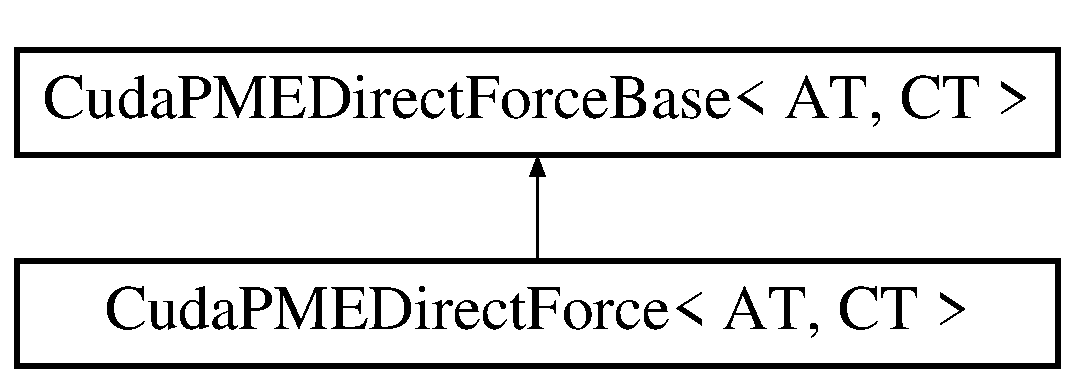
\includegraphics[height=2.000000cm]{classCudaPMEDirectForce}
\end{center}
\end{figure}
\subsection*{Public Member Functions}
\begin{DoxyCompactItemize}
\item 
\hypertarget{classCudaPMEDirectForce_a37a0656f51ce5edb079ac385a44ac343}{}\label{classCudaPMEDirectForce_a37a0656f51ce5edb079ac385a44ac343} 
{\bfseries Cuda\+P\+M\+E\+Direct\+Force} (\hyperlink{classCudaEnergyVirial}{Cuda\+Energy\+Virial} \&energy\+Virial, const char $\ast$name\+Vdw, const char $\ast$name\+Elec, const char $\ast$name\+Excl)
\item 
\hypertarget{classCudaPMEDirectForce_a75b212b3a1129a30ce0dcaf9da78f82a}{}\label{classCudaPMEDirectForce_a75b212b3a1129a30ce0dcaf9da78f82a} 
void {\bfseries setup} (double boxx, double boxy, double boxz, double kappa, double roff, double ron, double e14fac, int vdw\+\_\+model, int elec\+\_\+model)
\item 
\hypertarget{classCudaPMEDirectForce_aa10b0fc2ab0e030f9bd336b4d1cb4371}{}\label{classCudaPMEDirectForce_aa10b0fc2ab0e030f9bd336b4d1cb4371} 
void {\bfseries get\+\_\+setup} (float \&boxx, float \&boxy, float \&boxz, float \&kappa, float \&roff, float \&ron, float \&e14fac, int \&vdw\+\_\+model, int \&elec\+\_\+model)
\item 
\hypertarget{classCudaPMEDirectForce_a87260fe946f2deb76f0e46e3a175f43f}{}\label{classCudaPMEDirectForce_a87260fe946f2deb76f0e46e3a175f43f} 
void {\bfseries clear\+Textures} ()
\item 
\hypertarget{classCudaPMEDirectForce_a19b17fbe88dd50ed22d4bff34599cda6}{}\label{classCudaPMEDirectForce_a19b17fbe88dd50ed22d4bff34599cda6} 
void {\bfseries get\+\_\+box\+\_\+size} (CT \&boxx, CT \&boxy, CT \&boxz)
\item 
\hypertarget{classCudaPMEDirectForce_a5f079b84323cc87d6e00744753a868a1}{}\label{classCudaPMEDirectForce_a5f079b84323cc87d6e00744753a868a1} 
void {\bfseries set\+\_\+box\+\_\+size} (const CT boxx, const CT boxy, const CT boxz)
\item 
\hypertarget{classCudaPMEDirectForce_a167ba74f2475f5e2f5737adcde0f8bc0}{}\label{classCudaPMEDirectForce_a167ba74f2475f5e2f5737adcde0f8bc0} 
void {\bfseries set\+\_\+box\+\_\+size} (const double3 $\ast$d\+\_\+box\+Size)
\item 
\hypertarget{classCudaPMEDirectForce_ae3503a8806292af61d2a43225397f811}{}\label{classCudaPMEDirectForce_ae3503a8806292af61d2a43225397f811} 
void {\bfseries set\+\_\+calc\+\_\+vdw} (const bool calc\+\_\+vdw)
\item 
\hypertarget{classCudaPMEDirectForce_a5c4ad3a79e57c9212ddb43599fd604c5}{}\label{classCudaPMEDirectForce_a5c4ad3a79e57c9212ddb43599fd604c5} 
void {\bfseries set\+\_\+calc\+\_\+elec} (const bool calc\+\_\+elec)
\item 
\hypertarget{classCudaPMEDirectForce_a4ade5d2448929b9e16be7f70a95b069f}{}\label{classCudaPMEDirectForce_a4ade5d2448929b9e16be7f70a95b069f} 
bool {\bfseries get\+\_\+calc\+\_\+vdw} ()
\item 
\hypertarget{classCudaPMEDirectForce_a1672e6dbef6826e6a4a256a7eb355173}{}\label{classCudaPMEDirectForce_a1672e6dbef6826e6a4a256a7eb355173} 
bool {\bfseries get\+\_\+calc\+\_\+elec} ()
\item 
\hypertarget{classCudaPMEDirectForce_af371a75ded80c2dfed8af667f6ef91b5}{}\label{classCudaPMEDirectForce_af371a75ded80c2dfed8af667f6ef91b5} 
void {\bfseries set\+\_\+vdwparam} (const int nvdwparam, const CT $\ast$h\+\_\+vdwparam)
\item 
\hypertarget{classCudaPMEDirectForce_ac1cc762a417457f714b22086a745d4eb}{}\label{classCudaPMEDirectForce_ac1cc762a417457f714b22086a745d4eb} 
void {\bfseries set\+\_\+vdwparam} (const int nvdwparam, const char $\ast$filename)
\item 
\hypertarget{classCudaPMEDirectForce_a395020f6c963099db0253b0f7d99310a}{}\label{classCudaPMEDirectForce_a395020f6c963099db0253b0f7d99310a} 
void {\bfseries set\+\_\+vdwparam} (const std\+::vector$<$ CT $>$ vdwparam)
\item 
\hypertarget{classCudaPMEDirectForce_a8bd5f24897fdf3498d166b6c62354793}{}\label{classCudaPMEDirectForce_a8bd5f24897fdf3498d166b6c62354793} 
void {\bfseries set\+\_\+vdwparam14} (const int nvdwparam, const CT $\ast$h\+\_\+vdwparam)
\item 
\hypertarget{classCudaPMEDirectForce_af8544e4e8351069a16d2fd69c7ef2dac}{}\label{classCudaPMEDirectForce_af8544e4e8351069a16d2fd69c7ef2dac} 
void {\bfseries set\+\_\+vdwparam14} (const int nvdwparam, const char $\ast$filename)
\item 
\hypertarget{classCudaPMEDirectForce_a88fafb4e20fc47ed493b1dcb6f5fdf29}{}\label{classCudaPMEDirectForce_a88fafb4e20fc47ed493b1dcb6f5fdf29} 
void {\bfseries set\+\_\+vdwparam14} (const std\+::vector$<$ CT $>$ vdwparam)
\item 
\hypertarget{classCudaPMEDirectForce_a3afbd56eb0a15d10691636dc317e2014}{}\label{classCudaPMEDirectForce_a3afbd56eb0a15d10691636dc317e2014} 
void {\bfseries set\+\_\+vdwtype} (const int ncoord, const int $\ast$h\+\_\+vdwtype)
\item 
\hypertarget{classCudaPMEDirectForce_aa4632a6554912cb8097490e173172297}{}\label{classCudaPMEDirectForce_aa4632a6554912cb8097490e173172297} 
void {\bfseries set\+\_\+vdwtype14} (const int ncoord, const int $\ast$h\+\_\+vdwtype)
\item 
\hypertarget{classCudaPMEDirectForce_a8a9e4398177e64104eea3575f4ab8abb}{}\label{classCudaPMEDirectForce_a8a9e4398177e64104eea3575f4ab8abb} 
void {\bfseries set\+\_\+vdwtype} (const std\+::vector$<$ int $>$ \&vdw\+Type\+Vec)
\item 
\hypertarget{classCudaPMEDirectForce_a264e8631ff714bfd94ffd4f7419d2e23}{}\label{classCudaPMEDirectForce_a264e8631ff714bfd94ffd4f7419d2e23} 
void {\bfseries set\+\_\+vdwtype14} (const std\+::vector$<$ int $>$ \&vdw\+Type\+Vec)
\item 
\hypertarget{classCudaPMEDirectForce_a2dbd53823bcfcf2b4c400c1d50858505}{}\label{classCudaPMEDirectForce_a2dbd53823bcfcf2b4c400c1d50858505} 
void {\bfseries set\+\_\+vdwtype} (const int ncoord, const char $\ast$filename)
\item 
\hypertarget{classCudaPMEDirectForce_ae86a0371b56d11a043eae628adeaff11}{}\label{classCudaPMEDirectForce_ae86a0371b56d11a043eae628adeaff11} 
void {\bfseries set\+\_\+vdwtype14} (const int ncoord, const char $\ast$filename)
\item 
\hypertarget{classCudaPMEDirectForce_a156c597a81b36f606ae6ec678ee9d5d1}{}\label{classCudaPMEDirectForce_a156c597a81b36f606ae6ec678ee9d5d1} 
void {\bfseries set\+\_\+vdwtype} (const int ncoord, const int $\ast$glo\+\_\+vdwtype, const int $\ast$loc2glo, cuda\+Stream\+\_\+t stream=0)
\item 
\hypertarget{classCudaPMEDirectForce_a2f5d54d2fb17ceb9512f986068cba56f}{}\label{classCudaPMEDirectForce_a2f5d54d2fb17ceb9512f986068cba56f} 
void {\bfseries set\+\_\+sort\+\_\+vdwtype} (const int ncoord, const int $\ast$ind\+\_\+sorted, cuda\+Stream\+\_\+t stream=0)
\item 
\hypertarget{classCudaPMEDirectForce_a5e2f4c3126ce4b98f6ce2e5e74be5f0d}{}\label{classCudaPMEDirectForce_a5e2f4c3126ce4b98f6ce2e5e74be5f0d} 
void {\bfseries set\+\_\+sort\+\_\+vdwtype} (const int ncoord, const int $\ast$ind\+\_\+sorted)
\item 
\hypertarget{classCudaPMEDirectForce_ae52a39ad11c3d644a8ce9075e99dc2c2}{}\label{classCudaPMEDirectForce_ae52a39ad11c3d644a8ce9075e99dc2c2} 
void {\bfseries set\+\_\+14\+\_\+list} (int nin14list, int nex14list, \hyperlink{structxx14list__t}{xx14list\+\_\+t} $\ast$h\+\_\+in14list, \hyperlink{structxx14list__t}{xx14list\+\_\+t} $\ast$h\+\_\+ex14list, cuda\+Stream\+\_\+t stream=0)
\item 
\hypertarget{classCudaPMEDirectForce_aa56da928dbf9836e3af2b0d8d1b11a4a}{}\label{classCudaPMEDirectForce_aa56da928dbf9836e3af2b0d8d1b11a4a} 
void {\bfseries set\+\_\+14\+\_\+list} (std\+::string size\+File, std\+::string val\+File, cuda\+Stream\+\_\+t stream=0)
\item 
\hypertarget{classCudaPMEDirectForce_a0ab6c1ff2383bba0e7fbd4e2e42f00d7}{}\label{classCudaPMEDirectForce_a0ab6c1ff2383bba0e7fbd4e2e42f00d7} 
void {\bfseries set\+\_\+14\+\_\+list} (std\+::vector$<$ int $>$ size, std\+::vector$<$ int $>$ val, cuda\+Stream\+\_\+t stream=0)
\item 
\hypertarget{classCudaPMEDirectForce_a8b1cf6a999c187060b3480deb7cd3988}{}\label{classCudaPMEDirectForce_a8b1cf6a999c187060b3480deb7cd3988} 
void {\bfseries set\+\_\+14\+\_\+list} (const float4 $\ast$xyzq, const float boxx, const float boxy, const float boxz, const int $\ast$glo2loc\+\_\+ind, const int nin14\+\_\+tbl, const int $\ast$in14\+\_\+tbl, const \hyperlink{structxx14__t}{xx14\+\_\+t} $\ast$in14, const int nex14\+\_\+tbl, const int $\ast$ex14\+\_\+tbl, const \hyperlink{structxx14__t}{xx14\+\_\+t} $\ast$ex14, cuda\+Stream\+\_\+t stream=0)
\item 
\hypertarget{classCudaPMEDirectForce_ad1d326d6cbf3c5c0ce2341145e449b29}{}\label{classCudaPMEDirectForce_ad1d326d6cbf3c5c0ce2341145e449b29} 
void {\bfseries calc\+\_\+14\+\_\+force} (const float4 $\ast$xyzq, const bool calc\+\_\+energy, const bool calc\+\_\+virial, const int stride, AT $\ast$force, cuda\+Stream\+\_\+t stream=0)
\item 
\hypertarget{classCudaPMEDirectForce_aa194f6e6ecccb4f8642bd4a00d982e0a}{}\label{classCudaPMEDirectForce_aa194f6e6ecccb4f8642bd4a00d982e0a} 
void {\bfseries calc\+\_\+force} (const int whichlist, const float4 $\ast$xyzq, const \hyperlink{classCudaNeighborListBuild}{Cuda\+Neighbor\+List\+Build}$<$ 32 $>$ \&nlist, const bool calc\+\_\+energy, const bool calc\+\_\+virial, const int stride, AT $\ast$force, cuda\+Stream\+\_\+t stream=0)
\end{DoxyCompactItemize}
\subsection*{Protected Member Functions}
\begin{DoxyCompactItemize}
\item 
\hypertarget{classCudaPMEDirectForce_af8f3d155802b9cd8807acd32a1502854}{}\label{classCudaPMEDirectForce_af8f3d155802b9cd8807acd32a1502854} 
void {\bfseries setup\+\_\+ewald\+\_\+force} (CT h)
\item 
\hypertarget{classCudaPMEDirectForce_ac2921fbfcf6a69296b3a4f0113ba2ed6}{}\label{classCudaPMEDirectForce_ac2921fbfcf6a69296b3a4f0113ba2ed6} 
void {\bfseries set\+\_\+elec\+\_\+model} (int elec\+\_\+model, CT h=0.\+01)
\item 
\hypertarget{classCudaPMEDirectForce_a5eed2ed3e8255d16743912ffeebe69e2}{}\label{classCudaPMEDirectForce_a5eed2ed3e8255d16743912ffeebe69e2} 
void {\bfseries update\+\_\+setup} ()
\item 
\hypertarget{classCudaPMEDirectForce_a6d4629978da5717a081753a42c11ce1a}{}\label{classCudaPMEDirectForce_a6d4629978da5717a081753a42c11ce1a} 
void {\bfseries setup\+\_\+vdwparam} (const int type, const int nvdwparam, const CT $\ast$h\+\_\+vdwparam)
\item 
\hypertarget{classCudaPMEDirectForce_acda909dc533973ffa6d52a2b0a224fd3}{}\label{classCudaPMEDirectForce_acda909dc533973ffa6d52a2b0a224fd3} 
void {\bfseries load\+\_\+vdwparam} (const char $\ast$filename, const int nvdwparam, CT $\ast$$\ast$h\+\_\+vdwparam)
\end{DoxyCompactItemize}
\subsection*{Protected Attributes}
\begin{DoxyCompactItemize}
\item 
\hypertarget{classCudaPMEDirectForce_a9b9ff751f9d24b7ba63c56d3596ed7dd}{}\label{classCudaPMEDirectForce_a9b9ff751f9d24b7ba63c56d3596ed7dd} 
\hyperlink{classCudaEnergyVirial}{Cuda\+Energy\+Virial} \& {\bfseries energy\+Virial}
\item 
\hypertarget{classCudaPMEDirectForce_ad7d35fcba933d73734eae76acf44dc60}{}\label{classCudaPMEDirectForce_ad7d35fcba933d73734eae76acf44dc60} 
std\+::string {\bfseries str\+Vdw}
\item 
\hypertarget{classCudaPMEDirectForce_acad139531c45bed69454c6b3b9c7293a}{}\label{classCudaPMEDirectForce_acad139531c45bed69454c6b3b9c7293a} 
std\+::string {\bfseries str\+Elec}
\item 
\hypertarget{classCudaPMEDirectForce_a1b59c06d4ec1baee170b606eb4269134}{}\label{classCudaPMEDirectForce_a1b59c06d4ec1baee170b606eb4269134} 
std\+::string {\bfseries str\+Excl}
\item 
\hypertarget{classCudaPMEDirectForce_a58c55088e6a7a9d30b4657d35a912c62}{}\label{classCudaPMEDirectForce_a58c55088e6a7a9d30b4657d35a912c62} 
int {\bfseries nvdwparam}
\item 
\hypertarget{classCudaPMEDirectForce_a55394a57d60ed5d522e2804842b02293}{}\label{classCudaPMEDirectForce_a55394a57d60ed5d522e2804842b02293} 
int {\bfseries vdwparam\+\_\+len}
\item 
\hypertarget{classCudaPMEDirectForce_a6a430c208d010e9b8eabc4fefbcf8738}{}\label{classCudaPMEDirectForce_a6a430c208d010e9b8eabc4fefbcf8738} 
CT $\ast$ {\bfseries vdwparam}
\item 
\hypertarget{classCudaPMEDirectForce_a874707e9c8812e3f9650846d38c5c170}{}\label{classCudaPMEDirectForce_a874707e9c8812e3f9650846d38c5c170} 
const bool {\bfseries use\+\_\+tex\+\_\+vdwparam}
\item 
\hypertarget{classCudaPMEDirectForce_a08ea54ce0e7c25a10fc47d7fa20aa834}{}\label{classCudaPMEDirectForce_a08ea54ce0e7c25a10fc47d7fa20aa834} 
int {\bfseries nvdwparam14}
\item 
\hypertarget{classCudaPMEDirectForce_a9810606c5b67b8e1358a21dd52267b54}{}\label{classCudaPMEDirectForce_a9810606c5b67b8e1358a21dd52267b54} 
int {\bfseries vdwparam14\+\_\+len}
\item 
\hypertarget{classCudaPMEDirectForce_a642c827ebec2b4ee6091c0806e262ae0}{}\label{classCudaPMEDirectForce_a642c827ebec2b4ee6091c0806e262ae0} 
CT $\ast$ {\bfseries vdwparam14}
\item 
\hypertarget{classCudaPMEDirectForce_ac4023c8a6c50be1b41f87080bdab0194}{}\label{classCudaPMEDirectForce_ac4023c8a6c50be1b41f87080bdab0194} 
const bool {\bfseries use\+\_\+tex\+\_\+vdwparam14}
\item 
\hypertarget{classCudaPMEDirectForce_adf204871d75c3ec17adf97b6ba19d524}{}\label{classCudaPMEDirectForce_adf204871d75c3ec17adf97b6ba19d524} 
int {\bfseries nin14list}
\item 
\hypertarget{classCudaPMEDirectForce_a92377b204d75e191774541b68d40ded1}{}\label{classCudaPMEDirectForce_a92377b204d75e191774541b68d40ded1} 
int {\bfseries in14list\+\_\+len}
\item 
\hypertarget{classCudaPMEDirectForce_a3b4612cc39b7a1c4d27dc095d0817b9b}{}\label{classCudaPMEDirectForce_a3b4612cc39b7a1c4d27dc095d0817b9b} 
\hyperlink{structxx14list__t}{xx14list\+\_\+t} $\ast$ {\bfseries in14list}
\item 
\hypertarget{classCudaPMEDirectForce_a730b05258c0f99d09b1181869cb2b1c6}{}\label{classCudaPMEDirectForce_a730b05258c0f99d09b1181869cb2b1c6} 
int {\bfseries nex14list}
\item 
\hypertarget{classCudaPMEDirectForce_ab45c98a7e4d3031c2f945590d3aca20d}{}\label{classCudaPMEDirectForce_ab45c98a7e4d3031c2f945590d3aca20d} 
int {\bfseries ex14list\+\_\+len}
\item 
\hypertarget{classCudaPMEDirectForce_a773198e511dbbaad4823cc61afda9365}{}\label{classCudaPMEDirectForce_a773198e511dbbaad4823cc61afda9365} 
\hyperlink{structxx14list__t}{xx14list\+\_\+t} $\ast$ {\bfseries ex14list}
\item 
\hypertarget{classCudaPMEDirectForce_a4540a3e75aa6c7045c1b5a013a627b00}{}\label{classCudaPMEDirectForce_a4540a3e75aa6c7045c1b5a013a627b00} 
int {\bfseries vdwtype\+\_\+len}
\item 
\hypertarget{classCudaPMEDirectForce_ada2f2595d06925be4f06e053344e5663}{}\label{classCudaPMEDirectForce_ada2f2595d06925be4f06e053344e5663} 
int $\ast$ {\bfseries vdwtype}
\item 
\hypertarget{classCudaPMEDirectForce_acd5763d38ca84cca41213b7096de3a97}{}\label{classCudaPMEDirectForce_acd5763d38ca84cca41213b7096de3a97} 
int $\ast$ {\bfseries vdwtype14}
\item 
\hypertarget{classCudaPMEDirectForce_ab2591dd55c615fa945bc4e893993f4b8}{}\label{classCudaPMEDirectForce_ab2591dd55c615fa945bc4e893993f4b8} 
int $\ast$ {\bfseries vdwtype\+Temp}
\item 
\hypertarget{classCudaPMEDirectForce_a52986b92c802e949a89d30bc0ba13e0e}{}\label{classCudaPMEDirectForce_a52986b92c802e949a89d30bc0ba13e0e} 
int {\bfseries vdw\+\_\+model}
\item 
\hypertarget{classCudaPMEDirectForce_a51dd63375c1d2d7a0ce2bdd4e9b54fbd}{}\label{classCudaPMEDirectForce_a51dd63375c1d2d7a0ce2bdd4e9b54fbd} 
int {\bfseries elec\+\_\+model}
\item 
\hypertarget{classCudaPMEDirectForce_a06b0a24d8f633f58f9e871043e66b498}{}\label{classCudaPMEDirectForce_a06b0a24d8f633f58f9e871043e66b498} 
bool {\bfseries calc\+\_\+vdw}
\item 
\hypertarget{classCudaPMEDirectForce_aeea16163d9878c281ebb4ffb7a25b6fd}{}\label{classCudaPMEDirectForce_aeea16163d9878c281ebb4ffb7a25b6fd} 
bool {\bfseries calc\+\_\+elec}
\item 
\hypertarget{classCudaPMEDirectForce_a56269071dd0988ba22fcaa261130f635}{}\label{classCudaPMEDirectForce_a56269071dd0988ba22fcaa261130f635} 
CT $\ast$ {\bfseries ewald\+\_\+force}
\item 
\hypertarget{classCudaPMEDirectForce_a0d30e916d121a8937cc4ab6169c9fa08}{}\label{classCudaPMEDirectForce_a0d30e916d121a8937cc4ab6169c9fa08} 
int {\bfseries n\+\_\+ewald\+\_\+force}
\item 
\hypertarget{classCudaPMEDirectForce_a34fdb0fe96c7fe5d2967a61dc4871bf8}{}\label{classCudaPMEDirectForce_a34fdb0fe96c7fe5d2967a61dc4871bf8} 
\hyperlink{structDirectSettings__t}{Direct\+Settings\+\_\+t} $\ast$ {\bfseries h\+\_\+setup}
\end{DoxyCompactItemize}


The documentation for this class was generated from the following file\+:\begin{DoxyCompactItemize}
\item 
/u/samar/\+Documents/git/chcuda/include/Cuda\+P\+M\+E\+Direct\+Force.\+h\end{DoxyCompactItemize}

\hypertarget{classCudaPMEDirectForceBase}{}\section{Cuda\+P\+M\+E\+Direct\+Force\+Base$<$ AT, CT $>$ Class Template Reference}
\label{classCudaPMEDirectForceBase}\index{Cuda\+P\+M\+E\+Direct\+Force\+Base$<$ A\+T, C\+T $>$@{Cuda\+P\+M\+E\+Direct\+Force\+Base$<$ A\+T, C\+T $>$}}
Inheritance diagram for Cuda\+P\+M\+E\+Direct\+Force\+Base$<$ AT, CT $>$\+:\begin{figure}[H]
\begin{center}
\leavevmode
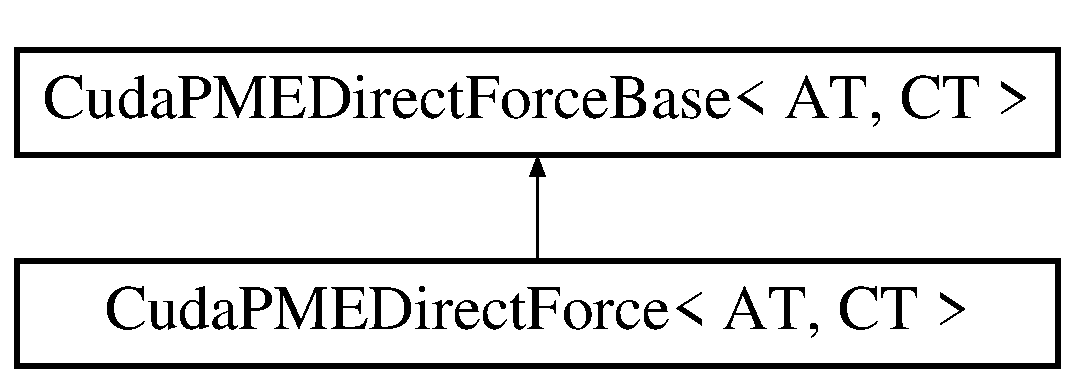
\includegraphics[height=2.000000cm]{classCudaPMEDirectForceBase}
\end{center}
\end{figure}
\subsection*{Public Member Functions}
\begin{DoxyCompactItemize}
\item 
\hypertarget{classCudaPMEDirectForceBase_a6e4bda7a4b887057ef166501efe1f5e3}{}\label{classCudaPMEDirectForceBase_a6e4bda7a4b887057ef166501efe1f5e3} 
virtual void {\bfseries setup} (double boxx, double boxy, double boxz, double kappa, double roff, double ron, double e14fac, int vdw\+\_\+model, int elec\+\_\+model)=0
\item 
\hypertarget{classCudaPMEDirectForceBase_afdbb13017b16e7badb33879a86e4b29b}{}\label{classCudaPMEDirectForceBase_afdbb13017b16e7badb33879a86e4b29b} 
virtual void {\bfseries get\+\_\+setup} (float \&boxx, float \&boxy, float \&boxz, float \&kappa, float \&roff, float \&ron, float \&e14fac, int \&vdw\+\_\+model, int \&elec\+\_\+model)=0
\item 
\hypertarget{classCudaPMEDirectForceBase_ace3a0538a11e847c206ca907930632ba}{}\label{classCudaPMEDirectForceBase_ace3a0538a11e847c206ca907930632ba} 
virtual void {\bfseries get\+\_\+box\+\_\+size} (CT \&boxx, CT \&boxy, CT \&boxz)=0
\item 
\hypertarget{classCudaPMEDirectForceBase_a79cecb72fc19f3cba6c56ea70188da9a}{}\label{classCudaPMEDirectForceBase_a79cecb72fc19f3cba6c56ea70188da9a} 
virtual void {\bfseries set\+\_\+box\+\_\+size} (const CT boxx, const CT boxy, const CT boxz)=0
\item 
\hypertarget{classCudaPMEDirectForceBase_a0c8f1fd6e11240463530a906b1a0d260}{}\label{classCudaPMEDirectForceBase_a0c8f1fd6e11240463530a906b1a0d260} 
virtual void {\bfseries set\+\_\+calc\+\_\+vdw} (const bool calc\+\_\+vdw)=0
\item 
\hypertarget{classCudaPMEDirectForceBase_ae8ea0ffc4fa34fa947cdace047111ea3}{}\label{classCudaPMEDirectForceBase_ae8ea0ffc4fa34fa947cdace047111ea3} 
virtual void {\bfseries set\+\_\+calc\+\_\+elec} (const bool calc\+\_\+elec)=0
\item 
\hypertarget{classCudaPMEDirectForceBase_a5bf42c88ac2bc32723eb538a523b3aad}{}\label{classCudaPMEDirectForceBase_a5bf42c88ac2bc32723eb538a523b3aad} 
virtual bool {\bfseries get\+\_\+calc\+\_\+vdw} ()=0
\item 
\hypertarget{classCudaPMEDirectForceBase_a9144d91225fcd7c84a9fe1a56b25119a}{}\label{classCudaPMEDirectForceBase_a9144d91225fcd7c84a9fe1a56b25119a} 
virtual bool {\bfseries get\+\_\+calc\+\_\+elec} ()=0
\item 
\hypertarget{classCudaPMEDirectForceBase_a202f784903e8444b04f2b943d8fb2a81}{}\label{classCudaPMEDirectForceBase_a202f784903e8444b04f2b943d8fb2a81} 
virtual void {\bfseries set\+\_\+vdwparam} (const int nvdwparam, const CT $\ast$h\+\_\+vdwparam)=0
\item 
\hypertarget{classCudaPMEDirectForceBase_af58b02699036a1a84d9caaf6e4b55f1c}{}\label{classCudaPMEDirectForceBase_af58b02699036a1a84d9caaf6e4b55f1c} 
virtual void {\bfseries set\+\_\+vdwparam} (const int nvdwparam, const char $\ast$filename)=0
\item 
\hypertarget{classCudaPMEDirectForceBase_ab65455bb482279b4b7287f347d88368d}{}\label{classCudaPMEDirectForceBase_ab65455bb482279b4b7287f347d88368d} 
virtual void {\bfseries set\+\_\+vdwparam14} (const int nvdwparam, const CT $\ast$h\+\_\+vdwparam)=0
\item 
\hypertarget{classCudaPMEDirectForceBase_a29398f2e91b8615e8161439f3d69c61b}{}\label{classCudaPMEDirectForceBase_a29398f2e91b8615e8161439f3d69c61b} 
virtual void {\bfseries set\+\_\+vdwparam14} (const int nvdwparam, const char $\ast$filename)=0
\item 
\hypertarget{classCudaPMEDirectForceBase_a8702e64c4c6994f40e29e6f665a8a79b}{}\label{classCudaPMEDirectForceBase_a8702e64c4c6994f40e29e6f665a8a79b} 
virtual void {\bfseries set\+\_\+vdwtype} (const int ncoord, const int $\ast$h\+\_\+vdwtype)=0
\item 
\hypertarget{classCudaPMEDirectForceBase_ad91c8d20c9cb7f8a96e5d3452c53534f}{}\label{classCudaPMEDirectForceBase_ad91c8d20c9cb7f8a96e5d3452c53534f} 
virtual void {\bfseries set\+\_\+vdwtype} (const int ncoord, const char $\ast$filename)=0
\item 
\hypertarget{classCudaPMEDirectForceBase_a93184411ca2fc4f89611e3c407d7d95f}{}\label{classCudaPMEDirectForceBase_a93184411ca2fc4f89611e3c407d7d95f} 
virtual void {\bfseries set\+\_\+vdwtype} (const int ncoord, const int $\ast$glo\+\_\+vdwtype, const int $\ast$loc2glo, cuda\+Stream\+\_\+t stream=0)=0
\item 
\hypertarget{classCudaPMEDirectForceBase_acdc1269a7448e495c4298c89603881e9}{}\label{classCudaPMEDirectForceBase_acdc1269a7448e495c4298c89603881e9} 
virtual void {\bfseries set\+\_\+14\+\_\+list} (int nin14list, int nex14list, \hyperlink{structxx14list__t}{xx14list\+\_\+t} $\ast$h\+\_\+in14list, \hyperlink{structxx14list__t}{xx14list\+\_\+t} $\ast$h\+\_\+ex14list, cuda\+Stream\+\_\+t stream=0)=0
\item 
\hypertarget{classCudaPMEDirectForceBase_a596d15a35fd6153ab187da5ae0a763d2}{}\label{classCudaPMEDirectForceBase_a596d15a35fd6153ab187da5ae0a763d2} 
virtual void {\bfseries set\+\_\+14\+\_\+list} (const float4 $\ast$xyzq, const float boxx, const float boxy, const float boxz, const int $\ast$glo2loc\+\_\+ind, const int nin14\+\_\+tbl, const int $\ast$in14\+\_\+tbl, const \hyperlink{structxx14__t}{xx14\+\_\+t} $\ast$in14, const int nex14\+\_\+tbl, const int $\ast$ex14\+\_\+tbl, const \hyperlink{structxx14__t}{xx14\+\_\+t} $\ast$ex14, cuda\+Stream\+\_\+t stream=0)=0
\item 
\hypertarget{classCudaPMEDirectForceBase_a537ecd649336b282e150995ca141ccb8}{}\label{classCudaPMEDirectForceBase_a537ecd649336b282e150995ca141ccb8} 
virtual void {\bfseries calc\+\_\+14\+\_\+force} (const float4 $\ast$xyzq, const bool calc\+\_\+energy, const bool calc\+\_\+virial, const int stride, AT $\ast$force, cuda\+Stream\+\_\+t stream=0)=0
\item 
\hypertarget{classCudaPMEDirectForceBase_a0484932e1c3d441f66b3b1ada4921e7d}{}\label{classCudaPMEDirectForceBase_a0484932e1c3d441f66b3b1ada4921e7d} 
virtual void {\bfseries calc\+\_\+force} (const int whichlist, const float4 $\ast$xyzq, const \hyperlink{classCudaNeighborListBuild}{Cuda\+Neighbor\+List\+Build}$<$ 32 $>$ \&nlist, const bool calc\+\_\+energy, const bool calc\+\_\+virial, const int stride, AT $\ast$force, cuda\+Stream\+\_\+t stream=0)=0
\end{DoxyCompactItemize}


The documentation for this class was generated from the following file\+:\begin{DoxyCompactItemize}
\item 
/u/samar/\+Documents/git/chcuda/include/Cuda\+P\+M\+E\+Direct\+Force.\+h\end{DoxyCompactItemize}

\hypertarget{classCudaPMERecip}{}\section{Cuda\+P\+M\+E\+Recip$<$ AT, CT, C\+T2 $>$ Class Template Reference}
\label{classCudaPMERecip}\index{Cuda\+P\+M\+E\+Recip$<$ A\+T, C\+T, C\+T2 $>$@{Cuda\+P\+M\+E\+Recip$<$ A\+T, C\+T, C\+T2 $>$}}
\subsection*{Public Member Functions}
\begin{DoxyCompactItemize}
\item 
\hypertarget{classCudaPMERecip_ab603d7df52a74df1ec8a297e7c7960ff}{}\label{classCudaPMERecip_ab603d7df52a74df1ec8a297e7c7960ff} 
{\bfseries Cuda\+P\+M\+E\+Recip} (\hyperlink{classCudaEnergyVirial}{Cuda\+Energy\+Virial} \&energy\+Virial)
\item 
\hypertarget{classCudaPMERecip_a8d7162c8b90917765687af7e9084022a}{}\label{classCudaPMERecip_a8d7162c8b90917765687af7e9084022a} 
{\bfseries Cuda\+P\+M\+E\+Recip} (int nfftx, int nffty, int nfftz, int order, F\+F\+Ttype fft\+\_\+type, int nnode, int mynode, \hyperlink{classCudaEnergyVirial}{Cuda\+Energy\+Virial} \&energy\+Virial, const char $\ast$name\+Recip, const char $\ast$name\+Self, cuda\+Stream\+\_\+t stream=0)
\item 
\hypertarget{classCudaPMERecip_aea4a4ba79bc3019bc42cb84edb484dc3}{}\label{classCudaPMERecip_aea4a4ba79bc3019bc42cb84edb484dc3} 
void {\bfseries set\+Params} (int nfft1, int nfft2, int nfft3, int ord)
\item 
\hypertarget{classCudaPMERecip_a44888114a2db33858b3c14bc0e2d4715}{}\label{classCudaPMERecip_a44888114a2db33858b3c14bc0e2d4715} 
void {\bfseries setup\+\_\+grid\+\_\+texture} (CT $\ast$data, const int data\+\_\+len)
\item 
\hypertarget{classCudaPMERecip_a68539c2121342493a6e1ed24c7cd24c3}{}\label{classCudaPMERecip_a68539c2121342493a6e1ed24c7cd24c3} 
void {\bfseries print\+\_\+info} ()
\item 
\hypertarget{classCudaPMERecip_ae9bd543d63eb7897a572e8a074bd3126}{}\label{classCudaPMERecip_ae9bd543d63eb7897a572e8a074bd3126} 
void {\bfseries set\+\_\+stream} (cuda\+Stream\+\_\+t stream)
\item 
\hypertarget{classCudaPMERecip_a4f1a154c20e19da29d785719956eef2b}{}\label{classCudaPMERecip_a4f1a154c20e19da29d785719956eef2b} 
void {\bfseries spread\+\_\+charge} (const int ncoord, const \hyperlink{classBspline}{Bspline}$<$ CT $>$ \&bspline)
\item 
\hypertarget{classCudaPMERecip_a2ae3f80940f7b2d3ded80a29650be9cf}{}\label{classCudaPMERecip_a2ae3f80940f7b2d3ded80a29650be9cf} 
void {\bfseries spread\+\_\+charge} (const float4 $\ast$xyzq, const int ncoord, const double $\ast$recip)
\item 
\hypertarget{classCudaPMERecip_a5a51525491c0ba1d6e6c941976333ae3}{}\label{classCudaPMERecip_a5a51525491c0ba1d6e6c941976333ae3} 
void {\bfseries spread\+\_\+charge\+\_\+block} (const float4 $\ast$xyzq, const int ncoord, const float $\ast$bixlam, const int $\ast$block\+Indexes, const double $\ast$recip)
\item 
\hypertarget{classCudaPMERecip_a62b0e684d24e90eb8073200eff211f54}{}\label{classCudaPMERecip_a62b0e684d24e90eb8073200eff211f54} 
void {\bfseries scalar\+\_\+sum} (const double $\ast$recip, const double kappa, const bool calc\+\_\+energy, const bool calc\+\_\+virial)
\item 
\hypertarget{classCudaPMERecip_a254ebf794806e929ee52c2afba4c5b1d}{}\label{classCudaPMERecip_a254ebf794806e929ee52c2afba4c5b1d} 
void {\bfseries calc\+\_\+self\+\_\+energy} (const float4 $\ast$xyzq, const int ncoord, const double kappa)
\item 
\hypertarget{classCudaPMERecip_a6e59ee35b534eefeba47a1bd2ccf6e4c}{}\label{classCudaPMERecip_a6e59ee35b534eefeba47a1bd2ccf6e4c} 
void {\bfseries calc\+\_\+self\+\_\+energy\+\_\+block} (const float4 $\ast$xyzq, const int ncoord, const double kappa, const float $\ast$bixlam, double $\ast$biflam, const int $\ast$block\+Indexes)
\item 
\hypertarget{classCudaPMERecip_a9851647dc81ec97299ec48757f758364}{}\label{classCudaPMERecip_a9851647dc81ec97299ec48757f758364} 
void {\bfseries gather\+\_\+force} (const int ncoord, const double $\ast$recip, const \hyperlink{classBspline}{Bspline}$<$ CT $>$ \&bspline, const int stride, CT $\ast$force)
\item 
\hypertarget{classCudaPMERecip_af4ae56f936724b33327b4b252f25a0cd}{}\label{classCudaPMERecip_af4ae56f936724b33327b4b252f25a0cd} 
{\footnotesize template$<$typename FT $>$ }\\void {\bfseries gather\+\_\+force} (const float4 $\ast$xyzq, const int ncoord, const double $\ast$recip, const int stride, FT $\ast$force)
\item 
\hypertarget{classCudaPMERecip_a1545f894c2fd03387dd159af7939a8e3}{}\label{classCudaPMERecip_a1545f894c2fd03387dd159af7939a8e3} 
{\footnotesize template$<$typename FT $>$ }\\void {\bfseries gather\+\_\+force\+\_\+block} (const float4 $\ast$xyzq, const int ncoord, const double $\ast$recip, const int stride, FT $\ast$force, const float $\ast$bixlam, double $\ast$biflam, const int $\ast$block\+Indexes)
\item 
\hypertarget{classCudaPMERecip_a7ec365cc8c4a9cb3cb5b58d575ebf40c}{}\label{classCudaPMERecip_a7ec365cc8c4a9cb3cb5b58d575ebf40c} 
void {\bfseries x\+\_\+fft\+\_\+r2c} (C\+T2 $\ast$data)
\item 
\hypertarget{classCudaPMERecip_af59edddef7fc70c6788594d7872b2001}{}\label{classCudaPMERecip_af59edddef7fc70c6788594d7872b2001} 
void {\bfseries x\+\_\+fft\+\_\+c2r} (C\+T2 $\ast$data)
\item 
\hypertarget{classCudaPMERecip_a3e83fe23990aa4501e64255473828ba5}{}\label{classCudaPMERecip_a3e83fe23990aa4501e64255473828ba5} 
void {\bfseries y\+\_\+fft\+\_\+c2c} (C\+T2 $\ast$data, const int direction)
\item 
\hypertarget{classCudaPMERecip_a86a345d67878a9f8d42bfc3c0eadbbd9}{}\label{classCudaPMERecip_a86a345d67878a9f8d42bfc3c0eadbbd9} 
void {\bfseries z\+\_\+fft\+\_\+c2c} (C\+T2 $\ast$data, const int direction)
\item 
\hypertarget{classCudaPMERecip_a7b6245521dd5912a5ec31c7c13f7433c}{}\label{classCudaPMERecip_a7b6245521dd5912a5ec31c7c13f7433c} 
void {\bfseries r2c\+\_\+fft} ()
\item 
\hypertarget{classCudaPMERecip_ae638f74b6074d4c50fdd41ff84a8bfdd}{}\label{classCudaPMERecip_ae638f74b6074d4c50fdd41ff84a8bfdd} 
void {\bfseries c2r\+\_\+fft} ()
\item 
\hypertarget{classCudaPMERecip_a6fdbe5f297b227e69d8cf7638012f296}{}\label{classCudaPMERecip_a6fdbe5f297b227e69d8cf7638012f296} 
int {\bfseries get\+\_\+nfftx} ()
\item 
\hypertarget{classCudaPMERecip_a16d048d9f9f23644a6021c45c685c0ef}{}\label{classCudaPMERecip_a16d048d9f9f23644a6021c45c685c0ef} 
int {\bfseries get\+\_\+nffty} ()
\item 
\hypertarget{classCudaPMERecip_a8380c164295fb5fe3f8c823b8c655b85}{}\label{classCudaPMERecip_a8380c164295fb5fe3f8c823b8c655b85} 
int {\bfseries get\+\_\+nfftz} ()
\item 
\hypertarget{classCudaPMERecip_a0bd7a8bb0e484230f3cb61b7d89f4104}{}\label{classCudaPMERecip_a0bd7a8bb0e484230f3cb61b7d89f4104} 
int {\bfseries get\+\_\+order} ()
\item 
\hypertarget{classCudaPMERecip_a5e1bca0437dbb6b876dcb8058dde326c}{}\label{classCudaPMERecip_a5e1bca0437dbb6b876dcb8058dde326c} 
void {\bfseries set\+\_\+order} (int order)
\end{DoxyCompactItemize}
\subsection*{Public Attributes}
\begin{DoxyCompactItemize}
\item 
\hypertarget{classCudaPMERecip_ae1147621dd9140cdb434b4a651ab0248}{}\label{classCudaPMERecip_ae1147621dd9140cdb434b4a651ab0248} 
CT $\ast$ {\bfseries data1}
\item 
\hypertarget{classCudaPMERecip_a4848c10367c77a2f9284b78fff736c8d}{}\label{classCudaPMERecip_a4848c10367c77a2f9284b78fff736c8d} 
CT $\ast$ {\bfseries data2}
\item 
\hypertarget{classCudaPMERecip_a50db202a7b64ef0b473bc298c4409fa8}{}\label{classCudaPMERecip_a50db202a7b64ef0b473bc298c4409fa8} 
int {\bfseries data1\+\_\+len}
\item 
\hypertarget{classCudaPMERecip_ad0e8bdffe5f64f58801622cbe80c4144}{}\label{classCudaPMERecip_ad0e8bdffe5f64f58801622cbe80c4144} 
int {\bfseries data2\+\_\+len}
\item 
\hypertarget{classCudaPMERecip_acbd804d0a5f6d7f03d55512b99e2f52c}{}\label{classCudaPMERecip_acbd804d0a5f6d7f03d55512b99e2f52c} 
F\+F\+Ttype {\bfseries fft\+\_\+type}
\item 
\hypertarget{classCudaPMERecip_ae632cdafcbb064958f5ddc0fee98b626}{}\label{classCudaPMERecip_ae632cdafcbb064958f5ddc0fee98b626} 
\hyperlink{classMatrix3d}{Matrix3d}$<$ AT $>$ $\ast$ {\bfseries accum\+\_\+grid}
\item 
\hypertarget{classCudaPMERecip_a638e85a71755377aa5f87f6f9d9558f3}{}\label{classCudaPMERecip_a638e85a71755377aa5f87f6f9d9558f3} 
\hyperlink{classMatrix3d}{Matrix3d}$<$ CT $>$ $\ast$ {\bfseries charge\+\_\+grid}
\item 
\hypertarget{classCudaPMERecip_a143ed80f1d166622e6ad21114e89661a}{}\label{classCudaPMERecip_a143ed80f1d166622e6ad21114e89661a} 
\hyperlink{classMatrix3d}{Matrix3d}$<$ CT $>$ $\ast$ {\bfseries solved\+\_\+grid}
\item 
\hypertarget{classCudaPMERecip_a1bcf6b29d30fb6b6e2ee5d7fe30bded1}{}\label{classCudaPMERecip_a1bcf6b29d30fb6b6e2ee5d7fe30bded1} 
\hyperlink{classMatrix3d}{Matrix3d}$<$ C\+T2 $>$ $\ast$ {\bfseries xfft\+\_\+grid}
\item 
\hypertarget{classCudaPMERecip_a0639f91d85ffdc0a1444395bec433902}{}\label{classCudaPMERecip_a0639f91d85ffdc0a1444395bec433902} 
\hyperlink{classMatrix3d}{Matrix3d}$<$ C\+T2 $>$ $\ast$ {\bfseries yfft\+\_\+grid}
\item 
\hypertarget{classCudaPMERecip_a9020023c824dbee5a04a39f62d6a4adc}{}\label{classCudaPMERecip_a9020023c824dbee5a04a39f62d6a4adc} 
\hyperlink{classMatrix3d}{Matrix3d}$<$ C\+T2 $>$ $\ast$ {\bfseries zfft\+\_\+grid}
\item 
\hypertarget{classCudaPMERecip_aa351fc06109560d4e4799647f0305e0d}{}\label{classCudaPMERecip_aa351fc06109560d4e4799647f0305e0d} 
\hyperlink{classMatrix3d}{Matrix3d}$<$ C\+T2 $>$ $\ast$ {\bfseries xyfft\+\_\+grid}
\item 
\hypertarget{classCudaPMERecip_ad55d7f051b50bf024eb02b9dacbc7f85}{}\label{classCudaPMERecip_ad55d7f051b50bf024eb02b9dacbc7f85} 
\hyperlink{classMatrix3d}{Matrix3d}$<$ C\+T2 $>$ $\ast$ {\bfseries fft\+\_\+grid}
\end{DoxyCompactItemize}


The documentation for this class was generated from the following file\+:\begin{DoxyCompactItemize}
\item 
/u/samar/\+Documents/git/chcuda/include/Cuda\+P\+M\+E\+Recip.\+h\end{DoxyCompactItemize}

\hypertarget{classCudaSimulationContext}{}\section{Cuda\+Simulation\+Context Class Reference}
\label{classCudaSimulationContext}\index{Cuda\+Simulation\+Context@{Cuda\+Simulation\+Context}}
\subsection*{Public Member Functions}
\begin{DoxyCompactItemize}
\item 
\hypertarget{classCudaSimulationContext_abb111e766ea4f2f5c26434909ff42684}{}\label{classCudaSimulationContext_abb111e766ea4f2f5c26434909ff42684} 
{\bfseries Cuda\+Simulation\+Context} (int num\+Atoms, double boxx\+\_\+in, double boxy\+\_\+in, double boxz\+\_\+in, uint64\+\_\+t seed)
\item 
\hypertarget{classCudaSimulationContext_ab0b762b45d6076be96bf3dd38ed1db70}{}\label{classCudaSimulationContext_ab0b762b45d6076be96bf3dd38ed1db70} 
void {\bfseries set\+Temperature} (const float temp)
\item 
\hypertarget{classCudaSimulationContext_a64a1d00b6efac2e9cde3b26923a2069c}{}\label{classCudaSimulationContext_a64a1d00b6efac2e9cde3b26923a2069c} 
float {\bfseries get\+Temperature} () const
\item 
\hypertarget{classCudaSimulationContext_a92681840f8841ae2b45566a85156efdd}{}\label{classCudaSimulationContext_a92681840f8841ae2b45566a85156efdd} 
void {\bfseries set\+Periodic\+Boundary\+Condition} (const P\+BC p)
\item 
\hypertarget{classCudaSimulationContext_aad2699c729bfbcc8c51fff0ed6745c2a}{}\label{classCudaSimulationContext_aad2699c729bfbcc8c51fff0ed6745c2a} 
P\+BC {\bfseries get\+Periodic\+Boundary\+Condition} () const
\item 
\hypertarget{classCudaSimulationContext_a3e7a34c3fd6f3fc0a4d53dd47ab43cd0}{}\label{classCudaSimulationContext_a3e7a34c3fd6f3fc0a4d53dd47ab43cd0} 
void {\bfseries set\+Coords} (std\+::vector$<$ float $>$ coords)
\item 
\hypertarget{classCudaSimulationContext_abcf10ad20bcfb62a1239b2f46f208e22}{}\label{classCudaSimulationContext_abcf10ad20bcfb62a1239b2f46f208e22} 
void {\bfseries set\+Charges} (std\+::vector$<$ float $>$ charges)
\item 
\hypertarget{classCudaSimulationContext_a16ac6180e3670440f97beeabd4baa350}{}\label{classCudaSimulationContext_a16ac6180e3670440f97beeabd4baa350} 
void {\bfseries set\+Periodic\+Box\+Sizes} (double x, double y, double z)
\item 
\hypertarget{classCudaSimulationContext_a8ce96a9eabd558ea3ffed21b2c515156}{}\label{classCudaSimulationContext_a8ce96a9eabd558ea3ffed21b2c515156} 
void {\bfseries set\+Piston} (double pressure, double pmass)
\item 
\hypertarget{classCudaSimulationContext_a96308a25437fb86cf88d5d7f59b560fc}{}\label{classCudaSimulationContext_a96308a25437fb86cf88d5d7f59b560fc} 
void {\bfseries set\+Masses} (const char $\ast$file\+Name)
\item 
\hypertarget{classCudaSimulationContext_a3b73f0eca80dd810e1bc593bc2ed2698}{}\label{classCudaSimulationContext_a3b73f0eca80dd810e1bc593bc2ed2698} 
void {\bfseries assign\+Velocities} ()
\item 
\hypertarget{classCudaSimulationContext_aeec06154411dccd89321fa2b594f20b9}{}\label{classCudaSimulationContext_aeec06154411dccd89321fa2b594f20b9} 
double {\bfseries calculate\+Potential\+Energy} (bool reset)
\item 
\hypertarget{classCudaSimulationContext_a1f25e0255919e0df3d49356b51ff3a0e}{}\label{classCudaSimulationContext_a1f25e0255919e0df3d49356b51ff3a0e} 
double {\bfseries calculate\+Potential\+Energy\+Print} (bool reset)
\item 
\hypertarget{classCudaSimulationContext_ad47a55e5a08360f5bb5bbdffc0c9e9dd}{}\label{classCudaSimulationContext_ad47a55e5a08360f5bb5bbdffc0c9e9dd} 
void {\bfseries calculate\+Kinetic\+Energy} ()
\item 
\hypertarget{classCudaSimulationContext_acdd86fc36567944c4433dc1616b0ac7a}{}\label{classCudaSimulationContext_acdd86fc36567944c4433dc1616b0ac7a} 
double $\ast$ {\bfseries get\+Forces} ()
\item 
void \hyperlink{classCudaSimulationContext_af8e340b880ef23301085fc702226c609}{move\+Forces\+To\+Dynamics} ()
\begin{DoxyCompactList}\small\item\em moves the calculated forces into force\+\_\+invmass array. \end{DoxyCompactList}\item 
void \hyperlink{classCudaSimulationContext_a3f3e6058db0acba85a440d9417c5e7e2}{move\+Positions\+To\+Energy} ()
\begin{DoxyCompactList}\small\item\em moves xyz into xyzq array. \end{DoxyCompactList}\item 
\hypertarget{classCudaSimulationContext_a2597d60c9f2eba81cbecc27430eb8af8}{}\label{classCudaSimulationContext_a2597d60c9f2eba81cbecc27430eb8af8} 
int {\bfseries get\+Num\+Atoms} () const
\item 
\hypertarget{classCudaSimulationContext_adebb325f8c0301463c0c711d9d27aede}{}\label{classCudaSimulationContext_adebb325f8c0301463c0c711d9d27aede} 
\hyperlink{classXYZQ}{X\+Y\+ZQ} $\ast$ {\bfseries get\+X\+Y\+ZQ} ()
\item 
\hypertarget{classCudaSimulationContext_a647a64eaf74697553611136883c87231}{}\label{classCudaSimulationContext_a647a64eaf74697553611136883c87231} 
int $\ast$ {\bfseries get\+\_\+loc2glo} () const
\item 
\hypertarget{classCudaSimulationContext_ab50cb50573965c0eb1d5cb721a469dd5}{}\label{classCudaSimulationContext_ab50cb50573965c0eb1d5cb721a469dd5} 
int {\bfseries get\+Force\+Stride} () const
\item 
uint64\+\_\+t \hyperlink{classCudaSimulationContext_ae52294d7e991824018cf9c9cb543ca1e}{get\+Seed} () const
\begin{DoxyCompactList}\small\item\em Seed for random number generator. \end{DoxyCompactList}\item 
\hypertarget{classCudaSimulationContext_aa4c1a2889174fa13b12cd1c5d51249ac}{}\label{classCudaSimulationContext_aa4c1a2889174fa13b12cd1c5d51249ac} 
void {\bfseries set\+Num\+Atoms} (const int num)
\item 
\hypertarget{classCudaSimulationContext_ace92f9f313550320d6e556f7d3545636}{}\label{classCudaSimulationContext_ace92f9f313550320d6e556f7d3545636} 
void {\bfseries set\+Topological\+Exclusions} (const int $\ast$iblo14, const int $\ast$inb14)
\item 
\hypertarget{classCudaSimulationContext_a248b72f769d347724512364558425d26}{}\label{classCudaSimulationContext_a248b72f769d347724512364558425d26} 
void {\bfseries set\+Reciprocal\+Space\+Parameters} (int nfft1, int nfft2, int nfft3, int pme\+Spline\+Order\+In, float kappa\+In)
\item 
\hypertarget{classCudaSimulationContext_a6a13d50ec17f5a8e286ea4d0694ddfdd}{}\label{classCudaSimulationContext_a6a13d50ec17f5a8e286ea4d0694ddfdd} 
void {\bfseries set\+Direct\+Space\+Parameters} (float cutoff\+In)
\item 
\hypertarget{classCudaSimulationContext_ae12349b0d0d27f4abefdde6e0b2e2e5a}{}\label{classCudaSimulationContext_ae12349b0d0d27f4abefdde6e0b2e2e5a} 
void {\bfseries set14\+Inclusion\+Exclusion} (const std\+::vector$<$ int $>$ \&in, const std\+::vector$<$ int $>$ \&ex)
\item 
\hypertarget{classCudaSimulationContext_a466032b2e7f0993d561216ecf4f645d8}{}\label{classCudaSimulationContext_a466032b2e7f0993d561216ecf4f645d8} 
void {\bfseries set\+Vdw\+Type} (const std\+::vector$<$ int $>$ \&vdw\+Type)
\item 
\hypertarget{classCudaSimulationContext_a470df687e207b0c118a1c7491532a40a}{}\label{classCudaSimulationContext_a470df687e207b0c118a1c7491532a40a} 
void {\bfseries set\+Vdw\+Param} (const std\+::vector$<$ float $>$ \&vdw\+Param)
\item 
\hypertarget{classCudaSimulationContext_a75c406ce602e5263c8614700d4da48e4}{}\label{classCudaSimulationContext_a75c406ce602e5263c8614700d4da48e4} 
void {\bfseries set\+Coords\+Charges} (const std\+::vector$<$ float4 $>$ \&coords\+Charges\+In)
\end{DoxyCompactItemize}
\subsection*{Public Attributes}
\begin{DoxyCompactItemize}
\item 
\hypertarget{classCudaSimulationContext_ae2c8c22913ba78d5ecaa6f939653b083}{}\label{classCudaSimulationContext_ae2c8c22913ba78d5ecaa6f939653b083} 
double $\ast$ {\bfseries d\+\_\+ke}
\item 
\hypertarget{classCudaSimulationContext_a5d41f0a61d810c2dd0abde6618800d02}{}\label{classCudaSimulationContext_a5d41f0a61d810c2dd0abde6618800d02} 
float {\bfseries boxx}
\item 
\hypertarget{classCudaSimulationContext_a3a5a2667d4317775fc338a3bad244dc9}{}\label{classCudaSimulationContext_a3a5a2667d4317775fc338a3bad244dc9} 
float {\bfseries boxy}
\item 
\hypertarget{classCudaSimulationContext_a3a0b09e28d233fff25f50f4f664b12d9}{}\label{classCudaSimulationContext_a3a0b09e28d233fff25f50f4f664b12d9} 
float {\bfseries boxz}
\item 
\hyperlink{structH__DVector}{H\+\_\+\+D\+Vector}$<$ uint64\+\_\+t $>$ \hyperlink{classCudaSimulationContext_aedf3a214b43fd5155f17ae8f3ce758e8}{randstep}
\begin{DoxyCompactList}\small\item\em random number step. \end{DoxyCompactList}\item 
\hyperlink{structVolumePiston}{Volume\+Piston} \hyperlink{classCudaSimulationContext_a9077736cc7f5dae5c741a2ebe7c21767}{piston}
\begin{DoxyCompactList}\small\item\em Volume piston used fro integrating the dynamcis of the box size. \end{DoxyCompactList}\item 
\hyperlink{structH__DVector}{H\+\_\+\+D\+Vector}$<$ double4 $>$ \hyperlink{classCudaSimulationContext_a861cbb2252066e6ed93a08d3dc908443}{force\+\_\+invmass}
\begin{DoxyCompactList}\small\item\em \hyperlink{classForce}{Force} and inverse of atom masses, used in dynamics to update velocities. \end{DoxyCompactList}\item 
\hyperlink{structH__DVector}{H\+\_\+\+D\+Vector}$<$ double4 $>$ \hyperlink{classCudaSimulationContext_af7492c16a26e127e9bc11d7e30d91ba7}{xyz}
\begin{DoxyCompactList}\small\item\em Positions of atoms, used in dynamics. \end{DoxyCompactList}\item 
\hyperlink{structH__DVector}{H\+\_\+\+D\+Vector}$<$ double4 $>$ \hyperlink{classCudaSimulationContext_a447bdf19525da955f30804b68a80efcf}{vel\+\_\+mass}
\begin{DoxyCompactList}\small\item\em Velocities and masses of atoms, used in dynamics. \end{DoxyCompactList}\item 
\hyperlink{structH__DVector}{H\+\_\+\+D\+Vector}$<$ double3 $>$ \hyperlink{classCudaSimulationContext_ab27a6d240361a27759e006728024e319}{box}
\begin{DoxyCompactList}\small\item\em Box dimentions, used in box piston dynamics. \end{DoxyCompactList}\item 
\hyperlink{structH__DVector}{H\+\_\+\+D\+Vector}$<$ double3 $>$ \hyperlink{classCudaSimulationContext_a2482b59305a454850b0d7d3e25f5830c}{box\+\_\+dot}
\begin{DoxyCompactList}\small\item\em Box dimensions time derivative, used in box piston dynamics. \end{DoxyCompactList}\item 
\hyperlink{structH__DVector}{H\+\_\+\+D\+Vector}$<$ double $>$ \hyperlink{classCudaSimulationContext_a353985244fa6f2dd2659120124f63bb5}{potential\+\_\+energy}
\begin{DoxyCompactList}\small\item\em Potential energy. \end{DoxyCompactList}\item 
\hyperlink{structH__DVector}{H\+\_\+\+D\+Vector}$<$ double3 $>$ \hyperlink{classCudaSimulationContext_a1f7666b2858c9720c33f04c67cd81302}{virial}
\begin{DoxyCompactList}\small\item\em Pressure group corrected virial, related to the change in energy given a small change in box size. \end{DoxyCompactList}\end{DoxyCompactItemize}


\subsection{Member Function Documentation}
\hypertarget{classCudaSimulationContext_ae52294d7e991824018cf9c9cb543ca1e}{}\label{classCudaSimulationContext_ae52294d7e991824018cf9c9cb543ca1e} 
\index{Cuda\+Simulation\+Context@{Cuda\+Simulation\+Context}!get\+Seed@{get\+Seed}}
\index{get\+Seed@{get\+Seed}!Cuda\+Simulation\+Context@{Cuda\+Simulation\+Context}}
\subsubsection{\texorpdfstring{get\+Seed()}{getSeed()}}
{\footnotesize\ttfamily uint64\+\_\+t Cuda\+Simulation\+Context\+::get\+Seed (\begin{DoxyParamCaption}{ }\end{DoxyParamCaption}) const\hspace{0.3cm}{\ttfamily [inline]}}



Seed for random number generator. 

This is used as the key for philox. \hypertarget{classCudaSimulationContext_af8e340b880ef23301085fc702226c609}{}\label{classCudaSimulationContext_af8e340b880ef23301085fc702226c609} 
\index{Cuda\+Simulation\+Context@{Cuda\+Simulation\+Context}!move\+Forces\+To\+Dynamics@{move\+Forces\+To\+Dynamics}}
\index{move\+Forces\+To\+Dynamics@{move\+Forces\+To\+Dynamics}!Cuda\+Simulation\+Context@{Cuda\+Simulation\+Context}}
\subsubsection{\texorpdfstring{move\+Forces\+To\+Dynamics()}{moveForcesToDynamics()}}
{\footnotesize\ttfamily void Cuda\+Simulation\+Context\+::move\+Forces\+To\+Dynamics (\begin{DoxyParamCaption}{ }\end{DoxyParamCaption})}



moves the calculated forces into force\+\_\+invmass array. 

\hypertarget{classCudaSimulationContext_a3f3e6058db0acba85a440d9417c5e7e2}{}\label{classCudaSimulationContext_a3f3e6058db0acba85a440d9417c5e7e2} 
\index{Cuda\+Simulation\+Context@{Cuda\+Simulation\+Context}!move\+Positions\+To\+Energy@{move\+Positions\+To\+Energy}}
\index{move\+Positions\+To\+Energy@{move\+Positions\+To\+Energy}!Cuda\+Simulation\+Context@{Cuda\+Simulation\+Context}}
\subsubsection{\texorpdfstring{move\+Positions\+To\+Energy()}{movePositionsToEnergy()}}
{\footnotesize\ttfamily void Cuda\+Simulation\+Context\+::move\+Positions\+To\+Energy (\begin{DoxyParamCaption}{ }\end{DoxyParamCaption})}



moves xyz into xyzq array. 



\subsection{Member Data Documentation}
\hypertarget{classCudaSimulationContext_ab27a6d240361a27759e006728024e319}{}\label{classCudaSimulationContext_ab27a6d240361a27759e006728024e319} 
\index{Cuda\+Simulation\+Context@{Cuda\+Simulation\+Context}!box@{box}}
\index{box@{box}!Cuda\+Simulation\+Context@{Cuda\+Simulation\+Context}}
\subsubsection{\texorpdfstring{box}{box}}
{\footnotesize\ttfamily \hyperlink{structH__DVector}{H\+\_\+\+D\+Vector}$<$double3$>$ Cuda\+Simulation\+Context\+::box}



Box dimentions, used in box piston dynamics. 

\hypertarget{classCudaSimulationContext_a2482b59305a454850b0d7d3e25f5830c}{}\label{classCudaSimulationContext_a2482b59305a454850b0d7d3e25f5830c} 
\index{Cuda\+Simulation\+Context@{Cuda\+Simulation\+Context}!box\+\_\+dot@{box\+\_\+dot}}
\index{box\+\_\+dot@{box\+\_\+dot}!Cuda\+Simulation\+Context@{Cuda\+Simulation\+Context}}
\subsubsection{\texorpdfstring{box\+\_\+dot}{box\_dot}}
{\footnotesize\ttfamily \hyperlink{structH__DVector}{H\+\_\+\+D\+Vector}$<$double3$>$ Cuda\+Simulation\+Context\+::box\+\_\+dot}



Box dimensions time derivative, used in box piston dynamics. 

\hypertarget{classCudaSimulationContext_a861cbb2252066e6ed93a08d3dc908443}{}\label{classCudaSimulationContext_a861cbb2252066e6ed93a08d3dc908443} 
\index{Cuda\+Simulation\+Context@{Cuda\+Simulation\+Context}!force\+\_\+invmass@{force\+\_\+invmass}}
\index{force\+\_\+invmass@{force\+\_\+invmass}!Cuda\+Simulation\+Context@{Cuda\+Simulation\+Context}}
\subsubsection{\texorpdfstring{force\+\_\+invmass}{force\_invmass}}
{\footnotesize\ttfamily \hyperlink{structH__DVector}{H\+\_\+\+D\+Vector}$<$double4$>$ Cuda\+Simulation\+Context\+::force\+\_\+invmass}



\hyperlink{classForce}{Force} and inverse of atom masses, used in dynamics to update velocities. 

\hypertarget{classCudaSimulationContext_a9077736cc7f5dae5c741a2ebe7c21767}{}\label{classCudaSimulationContext_a9077736cc7f5dae5c741a2ebe7c21767} 
\index{Cuda\+Simulation\+Context@{Cuda\+Simulation\+Context}!piston@{piston}}
\index{piston@{piston}!Cuda\+Simulation\+Context@{Cuda\+Simulation\+Context}}
\subsubsection{\texorpdfstring{piston}{piston}}
{\footnotesize\ttfamily \hyperlink{structVolumePiston}{Volume\+Piston} Cuda\+Simulation\+Context\+::piston}



Volume piston used fro integrating the dynamcis of the box size. 

\hypertarget{classCudaSimulationContext_a353985244fa6f2dd2659120124f63bb5}{}\label{classCudaSimulationContext_a353985244fa6f2dd2659120124f63bb5} 
\index{Cuda\+Simulation\+Context@{Cuda\+Simulation\+Context}!potential\+\_\+energy@{potential\+\_\+energy}}
\index{potential\+\_\+energy@{potential\+\_\+energy}!Cuda\+Simulation\+Context@{Cuda\+Simulation\+Context}}
\subsubsection{\texorpdfstring{potential\+\_\+energy}{potential\_energy}}
{\footnotesize\ttfamily \hyperlink{structH__DVector}{H\+\_\+\+D\+Vector}$<$double$>$ Cuda\+Simulation\+Context\+::potential\+\_\+energy}



Potential energy. 

\hypertarget{classCudaSimulationContext_aedf3a214b43fd5155f17ae8f3ce758e8}{}\label{classCudaSimulationContext_aedf3a214b43fd5155f17ae8f3ce758e8} 
\index{Cuda\+Simulation\+Context@{Cuda\+Simulation\+Context}!randstep@{randstep}}
\index{randstep@{randstep}!Cuda\+Simulation\+Context@{Cuda\+Simulation\+Context}}
\subsubsection{\texorpdfstring{randstep}{randstep}}
{\footnotesize\ttfamily \hyperlink{structH__DVector}{H\+\_\+\+D\+Vector}$<$uint64\+\_\+t$>$ Cuda\+Simulation\+Context\+::randstep}



random number step. 

Increment after a random kernel. Used for 64 msbs of the counter for philox. \hypertarget{classCudaSimulationContext_a447bdf19525da955f30804b68a80efcf}{}\label{classCudaSimulationContext_a447bdf19525da955f30804b68a80efcf} 
\index{Cuda\+Simulation\+Context@{Cuda\+Simulation\+Context}!vel\+\_\+mass@{vel\+\_\+mass}}
\index{vel\+\_\+mass@{vel\+\_\+mass}!Cuda\+Simulation\+Context@{Cuda\+Simulation\+Context}}
\subsubsection{\texorpdfstring{vel\+\_\+mass}{vel\_mass}}
{\footnotesize\ttfamily \hyperlink{structH__DVector}{H\+\_\+\+D\+Vector}$<$double4$>$ Cuda\+Simulation\+Context\+::vel\+\_\+mass}



Velocities and masses of atoms, used in dynamics. 

\hypertarget{classCudaSimulationContext_a1f7666b2858c9720c33f04c67cd81302}{}\label{classCudaSimulationContext_a1f7666b2858c9720c33f04c67cd81302} 
\index{Cuda\+Simulation\+Context@{Cuda\+Simulation\+Context}!virial@{virial}}
\index{virial@{virial}!Cuda\+Simulation\+Context@{Cuda\+Simulation\+Context}}
\subsubsection{\texorpdfstring{virial}{virial}}
{\footnotesize\ttfamily \hyperlink{structH__DVector}{H\+\_\+\+D\+Vector}$<$double3$>$ Cuda\+Simulation\+Context\+::virial}



Pressure group corrected virial, related to the change in energy given a small change in box size. 

\hypertarget{classCudaSimulationContext_af7492c16a26e127e9bc11d7e30d91ba7}{}\label{classCudaSimulationContext_af7492c16a26e127e9bc11d7e30d91ba7} 
\index{Cuda\+Simulation\+Context@{Cuda\+Simulation\+Context}!xyz@{xyz}}
\index{xyz@{xyz}!Cuda\+Simulation\+Context@{Cuda\+Simulation\+Context}}
\subsubsection{\texorpdfstring{xyz}{xyz}}
{\footnotesize\ttfamily \hyperlink{structH__DVector}{H\+\_\+\+D\+Vector}$<$double4$>$ Cuda\+Simulation\+Context\+::xyz}



Positions of atoms, used in dynamics. 



The documentation for this class was generated from the following file\+:\begin{DoxyCompactItemize}
\item 
/u/samar/\+Documents/git/chcuda/include/\hyperlink{CudaSimulationContext_8h}{Cuda\+Simulation\+Context.\+h}\end{DoxyCompactItemize}

\hypertarget{classCudaTopExcl}{}\section{Cuda\+Top\+Excl Class Reference}
\label{classCudaTopExcl}\index{Cuda\+Top\+Excl@{Cuda\+Top\+Excl}}
\subsection*{Public Member Functions}
\begin{DoxyCompactItemize}
\item 
\hypertarget{classCudaTopExcl_a5ec43fd8116eb88ecac9ea1c0cb54abf}{}\label{classCudaTopExcl_a5ec43fd8116eb88ecac9ea1c0cb54abf} 
{\bfseries Cuda\+Top\+Excl} (const int ncoord, const int $\ast$iblo14, const int $\ast$inb14)
\item 
\hypertarget{classCudaTopExcl_a2a244c80f305406b2d23d02874861793}{}\label{classCudaTopExcl_a2a244c80f305406b2d23d02874861793} 
{\bfseries Cuda\+Top\+Excl} (const int ncoord, std\+::string iblo14\+File, std\+::string inb14\+File)
\item 
\hypertarget{classCudaTopExcl_ad1371d59d9893fe18f13611c0dbf3ba3}{}\label{classCudaTopExcl_ad1371d59d9893fe18f13611c0dbf3ba3} 
void {\bfseries set\+From\+File} (const int num\+Atoms, std\+::string iblo14\+File, std\+::string inb14\+File)
\item 
\hypertarget{classCudaTopExcl_ad17c4599504dfd5c88a0529c3a49869b}{}\label{classCudaTopExcl_ad17c4599504dfd5c88a0529c3a49869b} 
void {\bfseries set\+From\+Pointers} (const int num\+Atoms, const int $\ast$iblo14, const int $\ast$inb14)
\item 
\hypertarget{classCudaTopExcl_a6bc858ee8d32017df14389fe28c5b9dd}{}\label{classCudaTopExcl_a6bc858ee8d32017df14389fe28c5b9dd} 
int {\bfseries get\+Atom\+Excl\+Pos\+Len} ()
\item 
\hypertarget{classCudaTopExcl_a4410c3045c751b928a25e72c690f9b7d}{}\label{classCudaTopExcl_a4410c3045c751b928a25e72c690f9b7d} 
int {\bfseries get\+Atom\+Excl\+Len} ()
\item 
\hypertarget{classCudaTopExcl_a6118b2743b391239be7a084b646f41bc}{}\label{classCudaTopExcl_a6118b2743b391239be7a084b646f41bc} 
int {\bfseries get\+Atom\+Excl\+Pos\+Len} () const
\item 
\hypertarget{classCudaTopExcl_ad17cec753b9afbe7fd582eec2fdd8ca2}{}\label{classCudaTopExcl_ad17cec753b9afbe7fd582eec2fdd8ca2} 
int {\bfseries get\+Atom\+Excl\+Len} () const
\item 
\hypertarget{classCudaTopExcl_af682699504552a77bb0f0223956009f0}{}\label{classCudaTopExcl_af682699504552a77bb0f0223956009f0} 
int $\ast$ {\bfseries get\+Atom\+Excl\+Pos} ()
\item 
\hypertarget{classCudaTopExcl_ac7a970603a83f633f3c5e57040358b37}{}\label{classCudaTopExcl_ac7a970603a83f633f3c5e57040358b37} 
int $\ast$ {\bfseries get\+Atom\+Excl} ()
\item 
\hypertarget{classCudaTopExcl_ac7839d5905cba6c34ca891307b7de592}{}\label{classCudaTopExcl_ac7839d5905cba6c34ca891307b7de592} 
const int $\ast$ {\bfseries get\+Atom\+Excl\+Pos} () const
\item 
\hypertarget{classCudaTopExcl_a597b4e31ea5293fcdb2f989e7e7b98e5}{}\label{classCudaTopExcl_a597b4e31ea5293fcdb2f989e7e7b98e5} 
const int $\ast$ {\bfseries get\+Atom\+Excl} () const
\item 
\hypertarget{classCudaTopExcl_a49cf43f096be49fafdc2857ca57a0076}{}\label{classCudaTopExcl_a49cf43f096be49fafdc2857ca57a0076} 
int {\bfseries get\+Max\+Num\+Excl} ()
\item 
\hypertarget{classCudaTopExcl_a89f802daabb4e3eb379d85578aa8ea49}{}\label{classCudaTopExcl_a89f802daabb4e3eb379d85578aa8ea49} 
int {\bfseries get\+Max\+Num\+Excl} () const
\item 
\hypertarget{classCudaTopExcl_a802965ac0e5c4d00e97fd76b192d481e}{}\label{classCudaTopExcl_a802965ac0e5c4d00e97fd76b192d481e} 
int {\bfseries get\+\_\+ncoord} ()
\item 
\hypertarget{classCudaTopExcl_a43a81b50052812d056a80aded50be2be}{}\label{classCudaTopExcl_a43a81b50052812d056a80aded50be2be} 
int {\bfseries get\+\_\+ncoord} () const
\item 
\hypertarget{classCudaTopExcl_ab202929b636b377210612aeda758030c}{}\label{classCudaTopExcl_ab202929b636b377210612aeda758030c} 
int $\ast$ {\bfseries get\+\_\+glo2loc} ()
\item 
\hypertarget{classCudaTopExcl_adf3155356d4a8c15748451193183b9b1}{}\label{classCudaTopExcl_adf3155356d4a8c15748451193183b9b1} 
int $\ast$ {\bfseries get\+\_\+glo2loc} () const
\end{DoxyCompactItemize}


The documentation for this class was generated from the following file\+:\begin{DoxyCompactItemize}
\item 
/u/samar/\+Documents/git/chcuda/include/Cuda\+Top\+Excl.\+h\end{DoxyCompactItemize}

\hypertarget{classCudaVerletIntegrator}{}\section{Cuda\+Verlet\+Integrator Class Reference}
\label{classCudaVerletIntegrator}\index{Cuda\+Verlet\+Integrator@{Cuda\+Verlet\+Integrator}}
Inheritance diagram for Cuda\+Verlet\+Integrator\+:\begin{figure}[H]
\begin{center}
\leavevmode
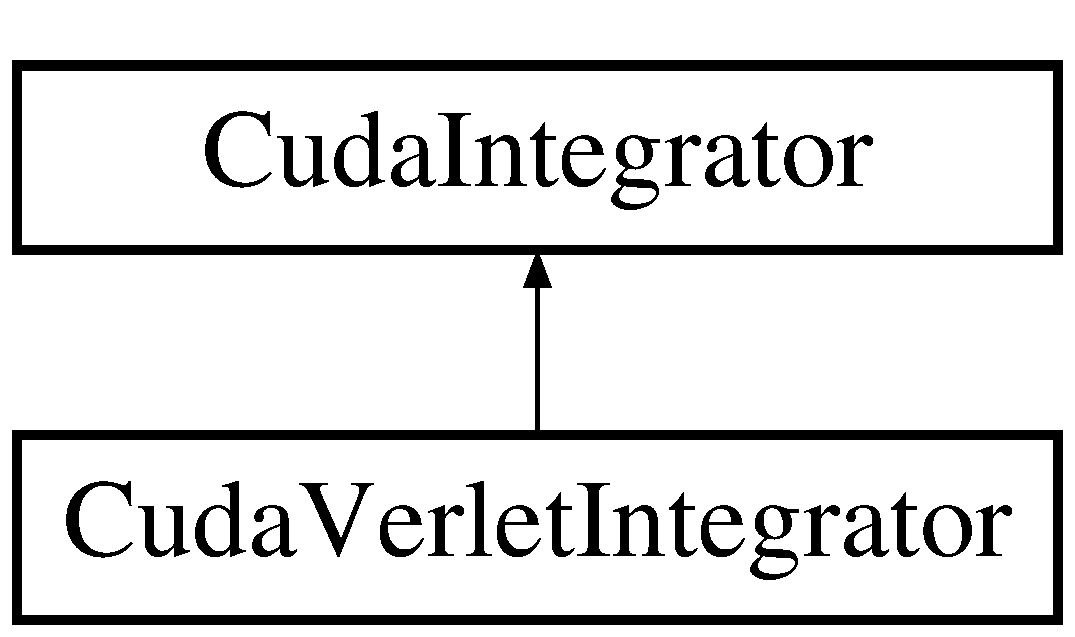
\includegraphics[height=2.000000cm]{classCudaVerletIntegrator}
\end{center}
\end{figure}
\subsection*{Public Member Functions}
\begin{DoxyCompactItemize}
\item 
\hypertarget{classCudaVerletIntegrator_a0e92c63dd2721d38d675ac512202189b}{}\label{classCudaVerletIntegrator_a0e92c63dd2721d38d675ac512202189b} 
{\bfseries Cuda\+Verlet\+Integrator} (double time\+Step)
\item 
\hypertarget{classCudaVerletIntegrator_aab3261c7210721b4e997d2ca5c6975a0}{}\label{classCudaVerletIntegrator_aab3261c7210721b4e997d2ca5c6975a0} 
void {\bfseries initialize} ()
\item 
\hypertarget{classCudaVerletIntegrator_a0ccbad0ff553021dfb6618e9e52f4f88}{}\label{classCudaVerletIntegrator_a0ccbad0ff553021dfb6618e9e52f4f88} 
void {\bfseries propagate} (int n\+Steps)
\end{DoxyCompactItemize}
\subsection*{Additional Inherited Members}


The documentation for this class was generated from the following file\+:\begin{DoxyCompactItemize}
\item 
/u/samar/\+Documents/git/chcuda/include/Cuda\+Verlet\+Integrator.\+h\end{DoxyCompactItemize}

\hypertarget{classcudaXYZ}{}\section{cuda\+X\+YZ$<$ T $>$ Class Template Reference}
\label{classcudaXYZ}\index{cuda\+X\+Y\+Z$<$ T $>$@{cuda\+X\+Y\+Z$<$ T $>$}}
Inheritance diagram for cuda\+X\+YZ$<$ T $>$\+:\begin{figure}[H]
\begin{center}
\leavevmode
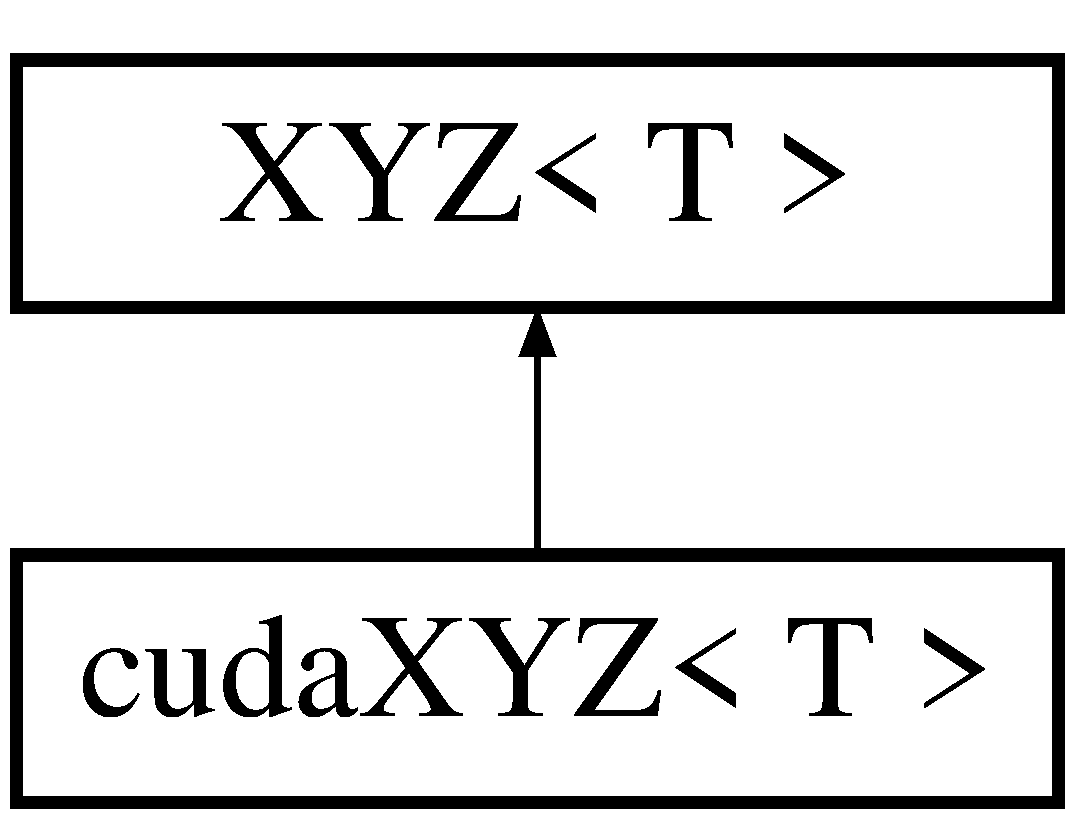
\includegraphics[height=2.000000cm]{classcudaXYZ}
\end{center}
\end{figure}
\subsection*{Public Member Functions}
\begin{DoxyCompactItemize}
\item 
\hypertarget{classcudaXYZ_a96f039e6dbc48700099c8bd46b4ea9cf}{}\label{classcudaXYZ_a96f039e6dbc48700099c8bd46b4ea9cf} 
{\bfseries cuda\+X\+YZ} (int size)
\item 
\hypertarget{classcudaXYZ_ab3983371d2c461fe9bc119a6cc51ea22}{}\label{classcudaXYZ_ab3983371d2c461fe9bc119a6cc51ea22} 
{\footnotesize template$<$typename P $>$ }\\{\bfseries cuda\+X\+YZ} (\hyperlink{classhostXYZ}{host\+X\+YZ}$<$ P $>$ \&xyz)
\item 
\hypertarget{classcudaXYZ_add2c4fc089505705e4b573a65808299a}{}\label{classcudaXYZ_add2c4fc089505705e4b573a65808299a} 
void {\bfseries realloc\+\_\+array} (T $\ast$$\ast$array, int $\ast$capacity, int size, float fac)
\item 
\hypertarget{classcudaXYZ_a3e91946cba1bb829af9b7fcd96752ba8}{}\label{classcudaXYZ_a3e91946cba1bb829af9b7fcd96752ba8} 
void {\bfseries resize\+\_\+array} (T $\ast$$\ast$array, int $\ast$capacity, int size, int new\+\_\+size, float fac)
\item 
\hypertarget{classcudaXYZ_a38e52631433135bb845803a615bbfd4f}{}\label{classcudaXYZ_a38e52631433135bb845803a615bbfd4f} 
void {\bfseries clear} (cuda\+Stream\+\_\+t stream=0)
\item 
\hypertarget{classcudaXYZ_a2494ea82dd6bc3baffe90526a532808f}{}\label{classcudaXYZ_a2494ea82dd6bc3baffe90526a532808f} 
{\footnotesize template$<$typename P $>$ }\\void {\bfseries set\+\_\+data} (\hyperlink{classhostXYZ}{host\+X\+YZ}$<$ P $>$ \&xyz, cuda\+Stream\+\_\+t stream=0)
\item 
\hypertarget{classcudaXYZ_a3eb7753507c67e944083a591e9fcda4c}{}\label{classcudaXYZ_a3eb7753507c67e944083a591e9fcda4c} 
{\footnotesize template$<$typename P $>$ }\\void {\bfseries set\+\_\+data\+\_\+sync} (\hyperlink{classhostXYZ}{host\+X\+YZ}$<$ P $>$ \&xyz)
\item 
\hypertarget{classcudaXYZ_a2d9ba6fa4e058e4a16de4dc45ae1cf99}{}\label{classcudaXYZ_a2d9ba6fa4e058e4a16de4dc45ae1cf99} 
{\footnotesize template$<$typename P $>$ }\\void {\bfseries set\+\_\+data} (\hyperlink{classcudaXYZ}{cuda\+X\+YZ}$<$ P $>$ \&xyz, cuda\+Stream\+\_\+t stream=0)
\item 
\hypertarget{classcudaXYZ_a0926b6a6b35b460d6a10f8258eb3401c}{}\label{classcudaXYZ_a0926b6a6b35b460d6a10f8258eb3401c} 
{\footnotesize template$<$typename P $>$ }\\void {\bfseries set\+\_\+data} (const int n, \hyperlink{classcudaXYZ}{cuda\+X\+YZ}$<$ P $>$ \&xyz, cuda\+Stream\+\_\+t stream=0)
\item 
\hypertarget{classcudaXYZ_a4071a8a5f90628273d6b9ab2826ae7bc}{}\label{classcudaXYZ_a4071a8a5f90628273d6b9ab2826ae7bc} 
{\footnotesize template$<$typename P $>$ }\\void {\bfseries set\+\_\+data\+\_\+sync} (\hyperlink{classcudaXYZ}{cuda\+X\+YZ}$<$ P $>$ \&xyz)
\item 
\hypertarget{classcudaXYZ_a9bbf30196c2c456695743efc0c4d0ece}{}\label{classcudaXYZ_a9bbf30196c2c456695743efc0c4d0ece} 
void {\bfseries set\+\_\+data\+\_\+sync} (const int size, const T $\ast$h\+\_\+x, const T $\ast$h\+\_\+y, const T $\ast$h\+\_\+z)
\item 
\hypertarget{classcudaXYZ_a7b374a4e611a9f24e4a7176c2cb237e3}{}\label{classcudaXYZ_a7b374a4e611a9f24e4a7176c2cb237e3} 
void {\bfseries set\+\_\+data\+\_\+sync} (const std\+::vector$<$ int $>$ \&h\+\_\+loc2glo, const T $\ast$h\+\_\+x, const T $\ast$h\+\_\+y, const T $\ast$h\+\_\+z)
\item 
\hypertarget{classcudaXYZ_ad5159dae798dea4cf39531dc383f8708}{}\label{classcudaXYZ_ad5159dae798dea4cf39531dc383f8708} 
void {\bfseries get\+\_\+data\+\_\+sync} (const int size, double $\ast$h\+\_\+x, double $\ast$h\+\_\+y, double $\ast$h\+\_\+z)
\item 
\hypertarget{classcudaXYZ_a6f8381bc6b76f10d827733ba12da74d1}{}\label{classcudaXYZ_a6f8381bc6b76f10d827733ba12da74d1} 
void {\bfseries get\+\_\+host\+\_\+xyz} (T $\ast$\&hx, T $\ast$\&hy, T $\ast$\&hz)
\item 
\hypertarget{classcudaXYZ_a9093eafba4c48b8c8d92a7072392231e}{}\label{classcudaXYZ_a9093eafba4c48b8c8d92a7072392231e} 
void {\bfseries release\+\_\+host\+\_\+xyz} (T $\ast$\&hx, T $\ast$\&hy, T $\ast$\&hz)
\end{DoxyCompactItemize}
\subsection*{Additional Inherited Members}


The documentation for this class was generated from the following file\+:\begin{DoxyCompactItemize}
\item 
/u/samar/\+Documents/git/chcuda/include/cuda\+X\+Y\+Z.\+h\end{DoxyCompactItemize}

\hypertarget{classdeviceVector}{}\section{device\+Vector$<$ T $>$ Class Template Reference}
\label{classdeviceVector}\index{device\+Vector$<$ T $>$@{device\+Vector$<$ T $>$}}
\subsection*{Public Member Functions}
\begin{DoxyCompactItemize}
\item 
\hypertarget{classdeviceVector_ac86c65e15ed22b7af8e5463cbee79eb6}{}\label{classdeviceVector_ac86c65e15ed22b7af8e5463cbee79eb6} 
{\bfseries device\+Vector} (size\+\_\+t size)
\item 
\hypertarget{classdeviceVector_a1a71678e2d829141c607cdd651c1c3f2}{}\label{classdeviceVector_a1a71678e2d829141c607cdd651c1c3f2} 
{\bfseries device\+Vector} (unsigned long long size)
\item 
\hypertarget{classdeviceVector_aa91a100e930ce5c2e49479bc688ce123}{}\label{classdeviceVector_aa91a100e930ce5c2e49479bc688ce123} 
void {\bfseries resize} (size\+\_\+t size)
\item 
\hypertarget{classdeviceVector_a1399a6e38bfd7b81560aedeab3335816}{}\label{classdeviceVector_a1399a6e38bfd7b81560aedeab3335816} 
T $\ast$ {\bfseries data} ()
\end{DoxyCompactItemize}


The documentation for this class was generated from the following file\+:\begin{DoxyCompactItemize}
\item 
/u/samar/\+Documents/git/chcuda/include/device\+Vector.\+h\end{DoxyCompactItemize}

\hypertarget{structdihe__t}{}\section{dihe\+\_\+t Struct Reference}
\label{structdihe__t}\index{dihe\+\_\+t@{dihe\+\_\+t}}
\subsection*{Public Member Functions}
\begin{DoxyCompactItemize}
\item 
\hypertarget{structdihe__t_ade6c45366819a0996cfac9622fd89fb5}{}\label{structdihe__t_ade6c45366819a0996cfac9622fd89fb5} 
void {\bfseries get\+Atoms} (std\+::vector$<$ int $>$ \&atoms)
\item 
\hypertarget{structdihe__t_a5235950b01a97a561430a1a0584e1c8e}{}\label{structdihe__t_a5235950b01a97a561430a1a0584e1c8e} 
void {\bfseries print\+Atoms} ()
\end{DoxyCompactItemize}
\subsection*{Static Public Member Functions}
\begin{DoxyCompactItemize}
\item 
\hypertarget{structdihe__t_ae81a1e7045fdb69e4efcfae1ae4cf285}{}\label{structdihe__t_ae81a1e7045fdb69e4efcfae1ae4cf285} 
static int {\bfseries type} ()
\item 
\hypertarget{structdihe__t_a7d19374e5c4898a9c7086fda751883c1}{}\label{structdihe__t_a7d19374e5c4898a9c7086fda751883c1} 
static int {\bfseries size} ()
\end{DoxyCompactItemize}
\subsection*{Public Attributes}
\begin{DoxyCompactItemize}
\item 
\hypertarget{structdihe__t_aedb872e978e947d7a260761a0222d321}{}\label{structdihe__t_aedb872e978e947d7a260761a0222d321} 
int {\bfseries i}
\item 
\hypertarget{structdihe__t_aa5dadfdf83f9e185cb57a4103354cd83}{}\label{structdihe__t_aa5dadfdf83f9e185cb57a4103354cd83} 
int {\bfseries j}
\item 
\hypertarget{structdihe__t_ab58a11dfd8ed89f043e923dc0af88d1c}{}\label{structdihe__t_ab58a11dfd8ed89f043e923dc0af88d1c} 
int {\bfseries k}
\item 
\hypertarget{structdihe__t_ab33df3bd4499ebd84abffe6ac7c16f89}{}\label{structdihe__t_ab33df3bd4499ebd84abffe6ac7c16f89} 
int {\bfseries l}
\item 
\hypertarget{structdihe__t_a6582249ff450110218e33099da98201e}{}\label{structdihe__t_a6582249ff450110218e33099da98201e} 
int {\bfseries itype}
\end{DoxyCompactItemize}


The documentation for this struct was generated from the following file\+:\begin{DoxyCompactItemize}
\item 
/u/samar/\+Documents/git/chcuda/include/Bonded\+\_\+struct.\+h\end{DoxyCompactItemize}

\hypertarget{structdihelist__t}{}\section{dihelist\+\_\+t Struct Reference}
\label{structdihelist__t}\index{dihelist\+\_\+t@{dihelist\+\_\+t}}
\subsection*{Public Attributes}
\begin{DoxyCompactItemize}
\item 
\hypertarget{structdihelist__t_ae8623fd40d55f8dffc0f6daf5a5a6bd7}{}\label{structdihelist__t_ae8623fd40d55f8dffc0f6daf5a5a6bd7} 
int {\bfseries i}
\item 
\hypertarget{structdihelist__t_a898323e38eee50f4627c82339b1d2915}{}\label{structdihelist__t_a898323e38eee50f4627c82339b1d2915} 
int {\bfseries j}
\item 
\hypertarget{structdihelist__t_a0b00c635d4b7a0f5934270554f96758e}{}\label{structdihelist__t_a0b00c635d4b7a0f5934270554f96758e} 
int {\bfseries k}
\item 
\hypertarget{structdihelist__t_a5e8e8adcfa59f5c1654ba2f5a589ce33}{}\label{structdihelist__t_a5e8e8adcfa59f5c1654ba2f5a589ce33} 
int {\bfseries l}
\item 
\hypertarget{structdihelist__t_af7c7f060c0b0674c6721c05bac090030}{}\label{structdihelist__t_af7c7f060c0b0674c6721c05bac090030} 
int {\bfseries itype}
\item 
\hypertarget{structdihelist__t_a3bc13b8f7ee08812e3cab31e37bec002}{}\label{structdihelist__t_a3bc13b8f7ee08812e3cab31e37bec002} 
int {\bfseries ishift1}
\item 
\hypertarget{structdihelist__t_a12d9bc73a51be26d49791cf9c9073fee}{}\label{structdihelist__t_a12d9bc73a51be26d49791cf9c9073fee} 
int {\bfseries ishift2}
\item 
\hypertarget{structdihelist__t_a3eae50b602d4ffb3402ab1162276853d}{}\label{structdihelist__t_a3eae50b602d4ffb3402ab1162276853d} 
int {\bfseries ishift3}
\end{DoxyCompactItemize}


The documentation for this struct was generated from the following file\+:\begin{DoxyCompactItemize}
\item 
/u/samar/\+Documents/git/chcuda/include/Bonded\+\_\+struct.\+h\end{DoxyCompactItemize}

\hypertarget{structDirectEnergyVirial__t}{}\section{Direct\+Energy\+Virial\+\_\+t Struct Reference}
\label{structDirectEnergyVirial__t}\index{Direct\+Energy\+Virial\+\_\+t@{Direct\+Energy\+Virial\+\_\+t}}
\subsection*{Public Attributes}
\begin{DoxyCompactItemize}
\item 
\hypertarget{structDirectEnergyVirial__t_a766eb3fbc4d353a23175b39cf16e7171}{}\label{structDirectEnergyVirial__t_a766eb3fbc4d353a23175b39cf16e7171} 
double {\bfseries energy\+\_\+vdw}
\item 
\hypertarget{structDirectEnergyVirial__t_a474244166132994ed765eb89f0647a10}{}\label{structDirectEnergyVirial__t_a474244166132994ed765eb89f0647a10} 
double {\bfseries energy\+\_\+elec}
\item 
\hypertarget{structDirectEnergyVirial__t_acd709c92f3ca421f07b176a656e4af11}{}\label{structDirectEnergyVirial__t_acd709c92f3ca421f07b176a656e4af11} 
double {\bfseries energy\+\_\+excl}
\item 
\hypertarget{structDirectEnergyVirial__t_a8395a2ecf98bda394c1443c060361aae}{}\label{structDirectEnergyVirial__t_a8395a2ecf98bda394c1443c060361aae} 
double {\bfseries vir} \mbox{[}9\mbox{]}
\item 
\hypertarget{structDirectEnergyVirial__t_a732ef30319dcef3b27fdaecb9e17f2f1}{}\label{structDirectEnergyVirial__t_a732ef30319dcef3b27fdaecb9e17f2f1} 
double {\bfseries sforce} \mbox{[}27 $\ast$3\mbox{]}
\item 
\hypertarget{structDirectEnergyVirial__t_afe9033e13c580c787ab064beba9731ec}{}\label{structDirectEnergyVirial__t_afe9033e13c580c787ab064beba9731ec} 
long long int {\bfseries sforce\+\_\+fp} \mbox{[}27 $\ast$3\mbox{]}
\end{DoxyCompactItemize}


The documentation for this struct was generated from the following file\+:\begin{DoxyCompactItemize}
\item 
/u/samar/\+Documents/git/chcuda/include/Cuda\+Direct\+Force\+Types.\+h\end{DoxyCompactItemize}

\hypertarget{structDirectSettings__t}{}\section{Direct\+Settings\+\_\+t Struct Reference}
\label{structDirectSettings__t}\index{Direct\+Settings\+\_\+t@{Direct\+Settings\+\_\+t}}
\subsection*{Public Attributes}
\begin{DoxyCompactItemize}
\item 
\hypertarget{structDirectSettings__t_ac690685545efdb10cc05c250c0634f7d}{}\label{structDirectSettings__t_ac690685545efdb10cc05c250c0634f7d} 
float {\bfseries kappa}
\item 
\hypertarget{structDirectSettings__t_a53ede6acd150841083aae5431a17150d}{}\label{structDirectSettings__t_a53ede6acd150841083aae5431a17150d} 
float {\bfseries kappa2}
\item 
\hypertarget{structDirectSettings__t_af22ab6924d4b2003884472f86b6f19b3}{}\label{structDirectSettings__t_af22ab6924d4b2003884472f86b6f19b3} 
float {\bfseries boxx}
\item 
\hypertarget{structDirectSettings__t_ac0e376e1741f1392e1b695d49cad1097}{}\label{structDirectSettings__t_ac0e376e1741f1392e1b695d49cad1097} 
float {\bfseries boxy}
\item 
\hypertarget{structDirectSettings__t_aa9fdea5c9d8edad28a7c1ae4aa1be8ea}{}\label{structDirectSettings__t_aa9fdea5c9d8edad28a7c1ae4aa1be8ea} 
float {\bfseries boxz}
\item 
\hypertarget{structDirectSettings__t_a29d92555be1811d5a97e62cb7a8bff90}{}\label{structDirectSettings__t_a29d92555be1811d5a97e62cb7a8bff90} 
float {\bfseries roff}
\item 
\hypertarget{structDirectSettings__t_af1e37b6f6e3209d69b9676fe7bb462db}{}\label{structDirectSettings__t_af1e37b6f6e3209d69b9676fe7bb462db} 
float {\bfseries roff2}
\item 
\hypertarget{structDirectSettings__t_ac47ba95d86b530f3a510f747ab1ed52c}{}\label{structDirectSettings__t_ac47ba95d86b530f3a510f747ab1ed52c} 
float {\bfseries roff3}
\item 
\hypertarget{structDirectSettings__t_a3e7f86660f9d2dcdcc7c503bea91d454}{}\label{structDirectSettings__t_a3e7f86660f9d2dcdcc7c503bea91d454} 
float {\bfseries roff5}
\item 
\hypertarget{structDirectSettings__t_a6f307552ea44aff0a21599e6ffe5ebbe}{}\label{structDirectSettings__t_a6f307552ea44aff0a21599e6ffe5ebbe} 
float {\bfseries ron}
\item 
\hypertarget{structDirectSettings__t_ae03618b642f64c23b80687db1d8001f0}{}\label{structDirectSettings__t_ae03618b642f64c23b80687db1d8001f0} 
float {\bfseries ron2}
\item 
\hypertarget{structDirectSettings__t_a75c7e74778c9475c618cb5dfff024b8a}{}\label{structDirectSettings__t_a75c7e74778c9475c618cb5dfff024b8a} 
float {\bfseries roffinv}
\item 
\hypertarget{structDirectSettings__t_a0ae8253411f50ca48f3fbfa1e0fe122f}{}\label{structDirectSettings__t_a0ae8253411f50ca48f3fbfa1e0fe122f} 
float {\bfseries roffinv2}
\item 
\hypertarget{structDirectSettings__t_a699fb58d315343d816c803ca3b261799}{}\label{structDirectSettings__t_a699fb58d315343d816c803ca3b261799} 
float {\bfseries roffinv3}
\item 
\hypertarget{structDirectSettings__t_ab981600e55d74a69b182e82247dda87f}{}\label{structDirectSettings__t_ab981600e55d74a69b182e82247dda87f} 
float {\bfseries roffinv4}
\item 
\hypertarget{structDirectSettings__t_a474229a9a6d739279ad20b8dad1d76b1}{}\label{structDirectSettings__t_a474229a9a6d739279ad20b8dad1d76b1} 
float {\bfseries roffinv5}
\item 
\hypertarget{structDirectSettings__t_ab7657e3f48658e519f990ed8de223842}{}\label{structDirectSettings__t_ab7657e3f48658e519f990ed8de223842} 
float {\bfseries roffinv6}
\item 
\hypertarget{structDirectSettings__t_a0868bf3c3f6021c1a90e8b2b6bf83e51}{}\label{structDirectSettings__t_a0868bf3c3f6021c1a90e8b2b6bf83e51} 
float {\bfseries roffinv12}
\item 
\hypertarget{structDirectSettings__t_ad8f03c70b7750e1edab0ac7113fb317c}{}\label{structDirectSettings__t_ad8f03c70b7750e1edab0ac7113fb317c} 
float {\bfseries roffinv18}
\item 
\hypertarget{structDirectSettings__t_ac80343b5986c42dbaed01d8ffea2dd66}{}\label{structDirectSettings__t_ac80343b5986c42dbaed01d8ffea2dd66} 
float {\bfseries inv\+\_\+roff2\+\_\+ron2\+\_\+3}
\item 
\hypertarget{structDirectSettings__t_a1085f30746665052d5c6c3124910abe3}{}\label{structDirectSettings__t_a1085f30746665052d5c6c3124910abe3} 
float {\bfseries k6}
\item 
\hypertarget{structDirectSettings__t_a60cb49cf0df76896f2c69e0f39f75935}{}\label{structDirectSettings__t_a60cb49cf0df76896f2c69e0f39f75935} 
float {\bfseries k12}
\item 
\hypertarget{structDirectSettings__t_a4a67bc0f8aae16ee23d884c5e6090e69}{}\label{structDirectSettings__t_a4a67bc0f8aae16ee23d884c5e6090e69} 
float {\bfseries dv6}
\item 
\hypertarget{structDirectSettings__t_ac5ffc6a3477a46381dae3808c4576bcf}{}\label{structDirectSettings__t_ac5ffc6a3477a46381dae3808c4576bcf} 
float {\bfseries dv12}
\item 
\hypertarget{structDirectSettings__t_aeda31cd21c664dd3078398612375f68d}{}\label{structDirectSettings__t_aeda31cd21c664dd3078398612375f68d} 
float {\bfseries ga6}
\item 
\hypertarget{structDirectSettings__t_abb44e014cff38fea4fd64195a2c84b37}{}\label{structDirectSettings__t_abb44e014cff38fea4fd64195a2c84b37} 
float {\bfseries gb6}
\item 
\hypertarget{structDirectSettings__t_a5208c523e140a6e3b7bf62002c358124}{}\label{structDirectSettings__t_a5208c523e140a6e3b7bf62002c358124} 
float {\bfseries gc6}
\item 
\hypertarget{structDirectSettings__t_a8c83298120f3bc428159689e879de85f}{}\label{structDirectSettings__t_a8c83298120f3bc428159689e879de85f} 
float {\bfseries ga12}
\item 
\hypertarget{structDirectSettings__t_a02265254ee8e2b53c4e54bef5c685843}{}\label{structDirectSettings__t_a02265254ee8e2b53c4e54bef5c685843} 
float {\bfseries gb12}
\item 
\hypertarget{structDirectSettings__t_a7ba4af87e397facc4eaef6f3a89ee135}{}\label{structDirectSettings__t_a7ba4af87e397facc4eaef6f3a89ee135} 
float {\bfseries gc12}
\item 
\hypertarget{structDirectSettings__t_a50b3ca9cf5dd51339122e4b11d0bc450}{}\label{structDirectSettings__t_a50b3ca9cf5dd51339122e4b11d0bc450} 
float {\bfseries G\+Aconst}
\item 
\hypertarget{structDirectSettings__t_a7b70c884e1c7baffa8956e3906520b4b}{}\label{structDirectSettings__t_a7b70c884e1c7baffa8956e3906520b4b} 
float {\bfseries G\+Bcoef}
\item 
\hypertarget{structDirectSettings__t_a006570ae8fd45ca08ccb2f28bebe2ea5}{}\label{structDirectSettings__t_a006570ae8fd45ca08ccb2f28bebe2ea5} 
float {\bfseries Aconst}
\item 
\hypertarget{structDirectSettings__t_a2269bc47262a0ca3073165d9f668defe}{}\label{structDirectSettings__t_a2269bc47262a0ca3073165d9f668defe} 
float {\bfseries Bconst}
\item 
\hypertarget{structDirectSettings__t_adb869c83d222c8416e4855ec63484b3c}{}\label{structDirectSettings__t_adb869c83d222c8416e4855ec63484b3c} 
float {\bfseries Cconst}
\item 
\hypertarget{structDirectSettings__t_a8df6cc6bfd088de06996dc5b6dad8dcd}{}\label{structDirectSettings__t_a8df6cc6bfd088de06996dc5b6dad8dcd} 
float {\bfseries Dconst}
\item 
\hypertarget{structDirectSettings__t_a12d192af6a3e1ec848762e5fa10be627}{}\label{structDirectSettings__t_a12d192af6a3e1ec848762e5fa10be627} 
float {\bfseries dvc}
\item 
\hypertarget{structDirectSettings__t_af7b01c3fa3db48008a3f990236f618d3}{}\label{structDirectSettings__t_af7b01c3fa3db48008a3f990236f618d3} 
float {\bfseries Acoef}
\item 
\hypertarget{structDirectSettings__t_a484aa6c211322d439d1f48411b6338b4}{}\label{structDirectSettings__t_a484aa6c211322d439d1f48411b6338b4} 
float {\bfseries Bcoef}
\item 
\hypertarget{structDirectSettings__t_ab11224012322d916579223ccde6dc4cf}{}\label{structDirectSettings__t_ab11224012322d916579223ccde6dc4cf} 
float {\bfseries Ccoef}
\item 
\hypertarget{structDirectSettings__t_ac7a18a12bca050572a20b5f6423360f4}{}\label{structDirectSettings__t_ac7a18a12bca050572a20b5f6423360f4} 
float {\bfseries Denom}
\item 
\hypertarget{structDirectSettings__t_a5e58f8f291da9dbfa565d12b49d247f5}{}\label{structDirectSettings__t_a5e58f8f291da9dbfa565d12b49d247f5} 
float {\bfseries Eaddr}
\item 
\hypertarget{structDirectSettings__t_a2bcb109b23a7346c941a7ce857442568}{}\label{structDirectSettings__t_a2bcb109b23a7346c941a7ce857442568} 
float {\bfseries Constr}
\item 
\hypertarget{structDirectSettings__t_a67250c768a1cec1a05d759e395293046}{}\label{structDirectSettings__t_a67250c768a1cec1a05d759e395293046} 
float {\bfseries e14fac}
\item 
\hypertarget{structDirectSettings__t_ac4c7569da2b9b9964e75992b5251d70a}{}\label{structDirectSettings__t_ac4c7569da2b9b9964e75992b5251d70a} 
float {\bfseries hinv}
\item 
\hypertarget{structDirectSettings__t_ae3710b1e4dc693eda79f62280406a6c3}{}\label{structDirectSettings__t_ae3710b1e4dc693eda79f62280406a6c3} 
float $\ast$ {\bfseries ewald\+\_\+force}
\end{DoxyCompactItemize}


The documentation for this struct was generated from the following file\+:\begin{DoxyCompactItemize}
\item 
/u/samar/\+Documents/git/chcuda/include/Cuda\+Direct\+Force\+Types.\+h\end{DoxyCompactItemize}

\hypertarget{classDomdecRecip}{}\section{Domdec\+Recip Class Reference}
\label{classDomdecRecip}\index{Domdec\+Recip@{Domdec\+Recip}}
Inheritance diagram for Domdec\+Recip\+:\begin{figure}[H]
\begin{center}
\leavevmode
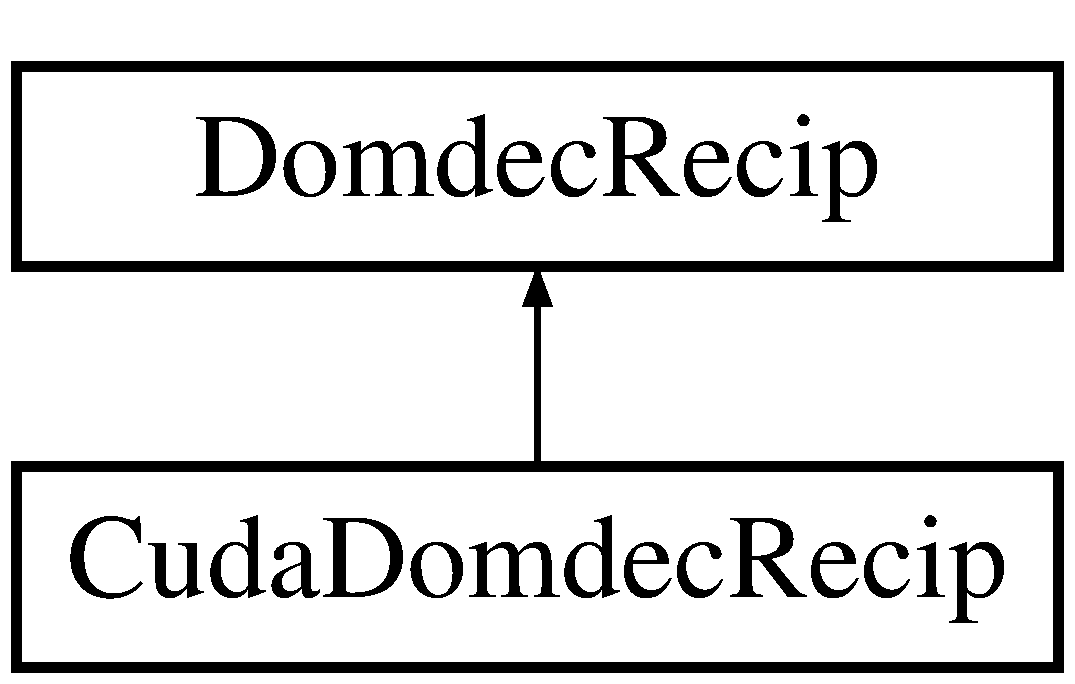
\includegraphics[height=2.000000cm]{classDomdecRecip}
\end{center}
\end{figure}
\subsection*{Public Member Functions}
\begin{DoxyCompactItemize}
\item 
\hypertarget{classDomdecRecip_a615297bad8615e487e032724af9e5f71}{}\label{classDomdecRecip_a615297bad8615e487e032724af9e5f71} 
{\bfseries Domdec\+Recip} (const int nfftx, const int nffty, const int nfftz, const int order, const double kappa)
\end{DoxyCompactItemize}
\subsection*{Protected Attributes}
\begin{DoxyCompactItemize}
\item 
\hypertarget{classDomdecRecip_a4c285af461282131d49ce72d35a85f42}{}\label{classDomdecRecip_a4c285af461282131d49ce72d35a85f42} 
int {\bfseries nfftx}
\item 
\hypertarget{classDomdecRecip_a7238cf29a27789310b2cefd4322d1fcb}{}\label{classDomdecRecip_a7238cf29a27789310b2cefd4322d1fcb} 
int {\bfseries nffty}
\item 
\hypertarget{classDomdecRecip_a87ae46c2f9f767aa5ae862a539be0454}{}\label{classDomdecRecip_a87ae46c2f9f767aa5ae862a539be0454} 
int {\bfseries nfftz}
\item 
\hypertarget{classDomdecRecip_afc932b2f968be556fb3685f9632e07fe}{}\label{classDomdecRecip_afc932b2f968be556fb3685f9632e07fe} 
int {\bfseries order}
\item 
\hypertarget{classDomdecRecip_a6169ef7da01efe0f6058cc8b0ad7985f}{}\label{classDomdecRecip_a6169ef7da01efe0f6058cc8b0ad7985f} 
double {\bfseries kappa}
\end{DoxyCompactItemize}


The documentation for this class was generated from the following file\+:\begin{DoxyCompactItemize}
\item 
/u/samar/\+Documents/git/chcuda/include/Domdec\+Recip.\+h\end{DoxyCompactItemize}

\hypertarget{structr123_1_1double2}{}\section{r123\+:\+:double2 Struct Reference}
\label{structr123_1_1double2}\index{r123\+::double2@{r123\+::double2}}
\subsection*{Public Attributes}
\begin{DoxyCompactItemize}
\item 
\hypertarget{structr123_1_1double2_a56bb85ee6730a9a30109b5db051fbd1b}{}\label{structr123_1_1double2_a56bb85ee6730a9a30109b5db051fbd1b} 
double {\bfseries x}
\item 
\hypertarget{structr123_1_1double2_a355ed766f070d275d7ad9268e15fb437}{}\label{structr123_1_1double2_a355ed766f070d275d7ad9268e15fb437} 
double {\bfseries y}
\end{DoxyCompactItemize}


The documentation for this struct was generated from the following file\+:\begin{DoxyCompactItemize}
\item 
/u/samar/\+Documents/git/chcuda/include/\+Random123/boxmuller.\+hpp\end{DoxyCompactItemize}

\hypertarget{classEnergyVirial}{}\section{Energy\+Virial Class Reference}
\label{classEnergyVirial}\index{Energy\+Virial@{Energy\+Virial}}
Inheritance diagram for Energy\+Virial\+:\begin{figure}[H]
\begin{center}
\leavevmode
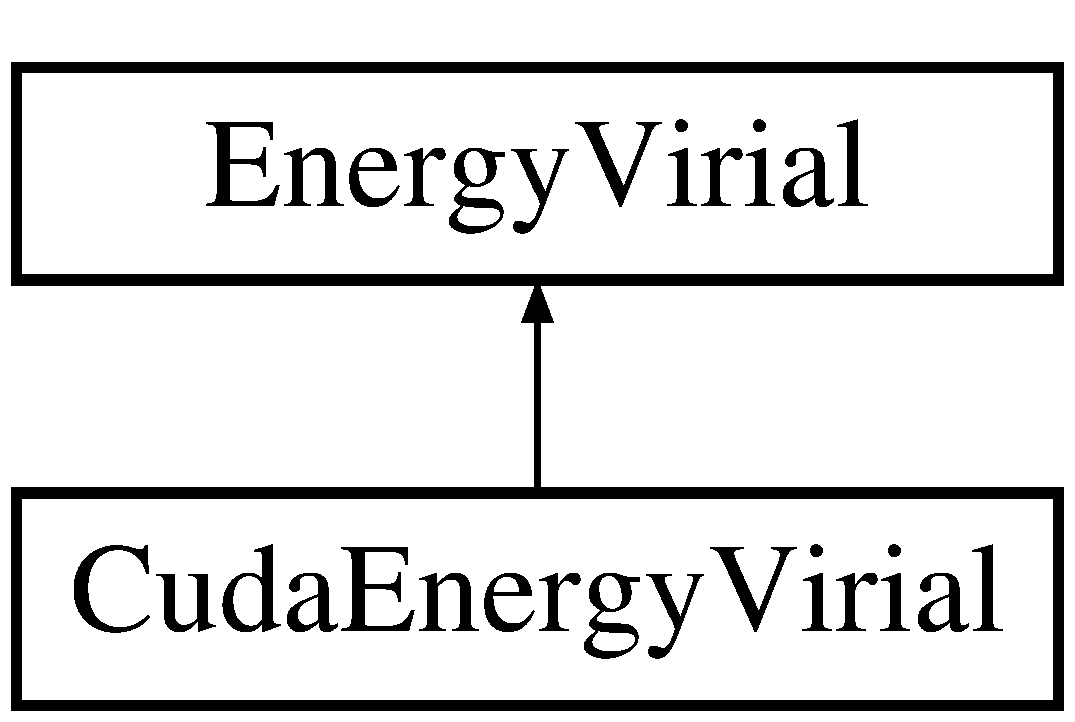
\includegraphics[height=2.000000cm]{classEnergyVirial}
\end{center}
\end{figure}
\subsection*{Public Member Functions}
\begin{DoxyCompactItemize}
\item 
\hypertarget{classEnergyVirial_ab0a01de91fea550a18be0b18fa9c8606}{}\label{classEnergyVirial_ab0a01de91fea550a18be0b18fa9c8606} 
void {\bfseries insert} (std\+::string \&name)
\item 
\hypertarget{classEnergyVirial_a4872fe5229c9a422bf7e5491cf2cda95}{}\label{classEnergyVirial_a4872fe5229c9a422bf7e5491cf2cda95} 
void {\bfseries insert} (const char $\ast$name)
\end{DoxyCompactItemize}
\subsection*{Protected Member Functions}
\begin{DoxyCompactItemize}
\item 
\hypertarget{classEnergyVirial_acc8c3f4db9dadd50ab4a1f92a7aa2554}{}\label{classEnergyVirial_acc8c3f4db9dadd50ab4a1f92a7aa2554} 
int {\bfseries get\+Energy\+Index} (std\+::string \&name)
\item 
\hypertarget{classEnergyVirial_abf03f7667ab45b697356b34df5b723e9}{}\label{classEnergyVirial_abf03f7667ab45b697356b34df5b723e9} 
int {\bfseries getN} ()
\end{DoxyCompactItemize}


The documentation for this class was generated from the following file\+:\begin{DoxyCompactItemize}
\item 
/u/samar/\+Documents/git/chcuda/include/Energy\+Virial.\+h\end{DoxyCompactItemize}

\hypertarget{structr123_1_1Engine}{}\section{r123\+:\+:Engine$<$ C\+B\+R\+NG $>$ Struct Template Reference}
\label{structr123_1_1Engine}\index{r123\+::\+Engine$<$ C\+B\+R\+N\+G $>$@{r123\+::\+Engine$<$ C\+B\+R\+N\+G $>$}}


If G satisfies the requirements of a C\+B\+R\+NG, and has a ctr\+\_\+type whose value\+\_\+type is an unsigned integral type, then Engine$<$\+G$>$ satisfies the requirements of a C++11 \char`\"{}\+Uniform Random Number Engine\char`\"{} and can be used in any context where such an object is expected.  




{\ttfamily \#include $<$Engine.\+hpp$>$}

\subsection*{Public Types}
\begin{DoxyCompactItemize}
\item 
\hypertarget{structr123_1_1Engine_a45ee0086cf8cd6d10febb76dc88f8b22}{}\label{structr123_1_1Engine_a45ee0086cf8cd6d10febb76dc88f8b22} 
typedef C\+B\+R\+NG {\bfseries cbrng\+\_\+type}
\item 
\hypertarget{structr123_1_1Engine_a96e0f5f039d5efd6aae77b63bafaad90}{}\label{structr123_1_1Engine_a96e0f5f039d5efd6aae77b63bafaad90} 
typedef C\+B\+R\+N\+G\+::ctr\+\_\+type {\bfseries ctr\+\_\+type}
\item 
\hypertarget{structr123_1_1Engine_a18132a79d2327990c4809b37300eddc3}{}\label{structr123_1_1Engine_a18132a79d2327990c4809b37300eddc3} 
typedef C\+B\+R\+N\+G\+::key\+\_\+type {\bfseries key\+\_\+type}
\item 
\hypertarget{structr123_1_1Engine_a32973bdda8697bcbb4dde11c0366a5e3}{}\label{structr123_1_1Engine_a32973bdda8697bcbb4dde11c0366a5e3} 
typedef C\+B\+R\+N\+G\+::ukey\+\_\+type {\bfseries ukey\+\_\+type}
\item 
\hypertarget{structr123_1_1Engine_a3d7cb66d43f99f5e227990af985ecb45}{}\label{structr123_1_1Engine_a3d7cb66d43f99f5e227990af985ecb45} 
typedef ctr\+\_\+type\+::value\+\_\+type {\bfseries result\+\_\+type}
\end{DoxyCompactItemize}
\subsection*{Public Member Functions}
\begin{DoxyCompactItemize}
\item 
\hypertarget{structr123_1_1Engine_ae1a249af828cfdac77db6c16e3f8f8eb}{}\label{structr123_1_1Engine_ae1a249af828cfdac77db6c16e3f8f8eb} 
{\bfseries Engine} (result\+\_\+type r)
\item 
\hypertarget{structr123_1_1Engine_a37dd55cee849b59d678f74780f785672}{}\label{structr123_1_1Engine_a37dd55cee849b59d678f74780f785672} 
{\bfseries Engine} (\hyperlink{structr123_1_1Engine}{Engine} \&e)
\item 
\hypertarget{structr123_1_1Engine_a478b486b166316597a51ffdd7b5b2d0c}{}\label{structr123_1_1Engine_a478b486b166316597a51ffdd7b5b2d0c} 
{\bfseries Engine} (const \hyperlink{structr123_1_1Engine}{Engine} \&e)
\item 
\hypertarget{structr123_1_1Engine_abd535170be11324a31b5657c2465d388}{}\label{structr123_1_1Engine_abd535170be11324a31b5657c2465d388} 
{\footnotesize template$<$typename Seed\+Seq $>$ }\\{\bfseries Engine} (Seed\+Seq \&s)
\item 
\hypertarget{structr123_1_1Engine_a93429593bdb12b202b4b8ed38fe08bc4}{}\label{structr123_1_1Engine_a93429593bdb12b202b4b8ed38fe08bc4} 
void {\bfseries seed} (result\+\_\+type r)
\item 
\hypertarget{structr123_1_1Engine_aac89ba287bdb118699c8eb8483c2c52a}{}\label{structr123_1_1Engine_aac89ba287bdb118699c8eb8483c2c52a} 
{\footnotesize template$<$typename Seed\+Seq $>$ }\\void {\bfseries seed} (Seed\+Seq \&s)
\item 
\hypertarget{structr123_1_1Engine_aff36bc97d11bc66f6c0edb75d8dc88e5}{}\label{structr123_1_1Engine_aff36bc97d11bc66f6c0edb75d8dc88e5} 
void {\bfseries seed} ()
\item 
\hypertarget{structr123_1_1Engine_aca309d0b4f2a8fff1f6f2ab38c6caf93}{}\label{structr123_1_1Engine_aca309d0b4f2a8fff1f6f2ab38c6caf93} 
result\+\_\+type {\bfseries operator()} ()
\item 
\hypertarget{structr123_1_1Engine_a3166cda5ff3d602244aef5dc96d489a4}{}\label{structr123_1_1Engine_a3166cda5ff3d602244aef5dc96d489a4} 
void {\bfseries discard} (R123\+\_\+\+U\+L\+O\+N\+G\+\_\+\+L\+O\+NG skip)
\item 
\hypertarget{structr123_1_1Engine_ab5f45b4eb97995cc45350abee3ec8388}{}\label{structr123_1_1Engine_ab5f45b4eb97995cc45350abee3ec8388} 
{\bfseries Engine} (const ukey\+\_\+type \&uk)
\item 
\hypertarget{structr123_1_1Engine_aeb178b9305cbf1fb7e11e8e33a631ba7}{}\label{structr123_1_1Engine_aeb178b9305cbf1fb7e11e8e33a631ba7} 
{\bfseries Engine} (ukey\+\_\+type \&uk)
\item 
\hypertarget{structr123_1_1Engine_a5c4d68dbbccfc71f467f3c902f5b93da}{}\label{structr123_1_1Engine_a5c4d68dbbccfc71f467f3c902f5b93da} 
void {\bfseries seed} (const ukey\+\_\+type \&uk)
\item 
\hypertarget{structr123_1_1Engine_a7bd6d3417cefb904c879f41d2c29e15e}{}\label{structr123_1_1Engine_a7bd6d3417cefb904c879f41d2c29e15e} 
void {\bfseries seed} (ukey\+\_\+type \&uk)
\item 
\hypertarget{structr123_1_1Engine_a4df4747f3b6129428537f6300e4b94c0}{}\label{structr123_1_1Engine_a4df4747f3b6129428537f6300e4b94c0} 
ctr\+\_\+type {\bfseries operator()} (const ctr\+\_\+type \&c) const
\item 
\hypertarget{structr123_1_1Engine_a807e0d14f7728978c63f4b88b7d1265f}{}\label{structr123_1_1Engine_a807e0d14f7728978c63f4b88b7d1265f} 
key\+\_\+type {\bfseries getkey} () const
\item 
\hypertarget{structr123_1_1Engine_ace8373d1ae2abf7849d4d9a983e63d07}{}\label{structr123_1_1Engine_ace8373d1ae2abf7849d4d9a983e63d07} 
void {\bfseries setkey} (const key\+\_\+type \&k)
\item 
\hypertarget{structr123_1_1Engine_a5e5b1e09ec6d17ad466bcf64293563c8}{}\label{structr123_1_1Engine_a5e5b1e09ec6d17ad466bcf64293563c8} 
std\+::pair$<$ ctr\+\_\+type, result\+\_\+type $>$ {\bfseries getcounter} () const
\item 
\hypertarget{structr123_1_1Engine_af078e04ceae8f975e9749d46a1d061f5}{}\label{structr123_1_1Engine_af078e04ceae8f975e9749d46a1d061f5} 
void {\bfseries setcounter} (const ctr\+\_\+type \&\+\_\+c, result\+\_\+type \+\_\+elem)
\item 
\hypertarget{structr123_1_1Engine_abb13a45ea570e48b1474a40dbcccd445}{}\label{structr123_1_1Engine_abb13a45ea570e48b1474a40dbcccd445} 
void {\bfseries setcounter} (const std\+::pair$<$ ctr\+\_\+type, result\+\_\+type $>$ \&ce)
\end{DoxyCompactItemize}
\subsection*{Static Public Member Functions}
\begin{DoxyCompactItemize}
\item 
\hypertarget{structr123_1_1Engine_af5441fc62932c3d099f8b16150d2aa81}{}\label{structr123_1_1Engine_af5441fc62932c3d099f8b16150d2aa81} 
static R123\+\_\+\+C\+O\+N\+S\+T\+E\+X\+PR result\+\_\+type min {\bfseries R123\+\_\+\+N\+O\+\_\+\+M\+A\+C\+R\+O\+\_\+\+S\+U\+B\+ST} ()
\item 
\hypertarget{structr123_1_1Engine_a112318f7d0015ecf4c3c6a8a5c76371b}{}\label{structr123_1_1Engine_a112318f7d0015ecf4c3c6a8a5c76371b} 
static R123\+\_\+\+C\+O\+N\+S\+T\+E\+X\+PR result\+\_\+type max {\bfseries R123\+\_\+\+N\+O\+\_\+\+M\+A\+C\+R\+O\+\_\+\+S\+U\+B\+ST} ()
\end{DoxyCompactItemize}
\subsection*{Static Public Attributes}
\begin{DoxyCompactItemize}
\item 
\hypertarget{structr123_1_1Engine_aa73e4d27847915f1438fd37b30777111}{}\label{structr123_1_1Engine_aa73e4d27847915f1438fd37b30777111} 
static const result\+\_\+type {\bfseries \+\_\+\+Min} = 0
\item 
\hypertarget{structr123_1_1Engine_ae549f81e966b0414bcaf0f24b566ebd8}{}\label{structr123_1_1Engine_ae549f81e966b0414bcaf0f24b566ebd8} 
static const result\+\_\+type {\bfseries \+\_\+\+Max} = $\sim$((result\+\_\+type)0)
\end{DoxyCompactItemize}
\subsection*{Protected Member Functions}
\begin{DoxyCompactItemize}
\item 
\hypertarget{structr123_1_1Engine_aa7ad87d7238a0f820ee37640071dee7d}{}\label{structr123_1_1Engine_aa7ad87d7238a0f820ee37640071dee7d} 
void {\bfseries fix\+\_\+invariant} ()
\end{DoxyCompactItemize}
\subsection*{Protected Attributes}
\begin{DoxyCompactItemize}
\item 
\hypertarget{structr123_1_1Engine_a5e430e850badcc4fd0f74de4a49a673b}{}\label{structr123_1_1Engine_a5e430e850badcc4fd0f74de4a49a673b} 
cbrng\+\_\+type {\bfseries b}
\item 
\hypertarget{structr123_1_1Engine_adb9e1841a81f213a115e9f092f5c4654}{}\label{structr123_1_1Engine_adb9e1841a81f213a115e9f092f5c4654} 
key\+\_\+type {\bfseries key}
\item 
\hypertarget{structr123_1_1Engine_afb056ed93053f4175aabc9f4e5dd7b8d}{}\label{structr123_1_1Engine_afb056ed93053f4175aabc9f4e5dd7b8d} 
ctr\+\_\+type {\bfseries c}
\item 
\hypertarget{structr123_1_1Engine_a6169d4fbce1fd7725fabda4c693bf250}{}\label{structr123_1_1Engine_a6169d4fbce1fd7725fabda4c693bf250} 
ctr\+\_\+type {\bfseries v}
\end{DoxyCompactItemize}
\subsection*{Friends}
\begin{DoxyCompactItemize}
\item 
\hypertarget{structr123_1_1Engine_a606e3ba824542e52f12df1345126e721}{}\label{structr123_1_1Engine_a606e3ba824542e52f12df1345126e721} 
bool {\bfseries operator==} (const \hyperlink{structr123_1_1Engine}{Engine} \&lhs, const \hyperlink{structr123_1_1Engine}{Engine} \&rhs)
\item 
\hypertarget{structr123_1_1Engine_af0947cdcfc03aef7ec30c9fafa660445}{}\label{structr123_1_1Engine_af0947cdcfc03aef7ec30c9fafa660445} 
bool {\bfseries operator!=} (const \hyperlink{structr123_1_1Engine}{Engine} \&lhs, const \hyperlink{structr123_1_1Engine}{Engine} \&rhs)
\item 
\hypertarget{structr123_1_1Engine_ae0321571f689fca00c608d11ecad7d8d}{}\label{structr123_1_1Engine_ae0321571f689fca00c608d11ecad7d8d} 
std\+::ostream \& {\bfseries operator$<$$<$} (std\+::ostream \&os, const \hyperlink{structr123_1_1Engine}{Engine} \&be)
\item 
\hypertarget{structr123_1_1Engine_ae708b771ab5ac17700d34bad875a16d9}{}\label{structr123_1_1Engine_ae708b771ab5ac17700d34bad875a16d9} 
std\+::istream \& {\bfseries operator$>$$>$} (std\+::istream \&is, \hyperlink{structr123_1_1Engine}{Engine} \&be)
\end{DoxyCompactItemize}


\subsection{Detailed Description}
\subsubsection*{template$<$typename C\+B\+R\+NG$>$\newline
struct r123\+::\+Engine$<$ C\+B\+R\+N\+G $>$}

If G satisfies the requirements of a C\+B\+R\+NG, and has a ctr\+\_\+type whose value\+\_\+type is an unsigned integral type, then Engine$<$\+G$>$ satisfies the requirements of a C++11 \char`\"{}\+Uniform Random Number Engine\char`\"{} and can be used in any context where such an object is expected. 

Note that wrapping a counter based R\+NG with a traditional A\+PI in this way obscures much of the power of counter based P\+R\+N\+Gs. Nevertheless, it may be of value in applications that are already coded to work with the C++11 random number engines.

The \hyperlink{classr123_1_1MicroURNG}{Micro\+U\+R\+NG} template in \hyperlink{MicroURNG_8hpp_source}{Micro\+U\+R\+N\+G.\+hpp} provides the more limited functionality of a C++11 \char`\"{}\+Uniform
\+Random Number Generator\char`\"{}, but leaves the application in control of counters and keys and hence may be preferable to the \hyperlink{structr123_1_1Engine}{Engine} template. For example, a \hyperlink{classr123_1_1MicroURNG}{Micro\+U\+R\+NG} allows one to use C++11 \char`\"{}\+Random Number
\+Distributions\char`\"{} without giving up control over the counters and keys. 

The documentation for this struct was generated from the following file\+:\begin{DoxyCompactItemize}
\item 
/u/samar/\+Documents/git/chcuda/include/\+Random123/conventional/Engine.\+hpp\end{DoxyCompactItemize}

\hypertarget{structr123_1_1float2}{}\section{r123\+:\+:float2 Struct Reference}
\label{structr123_1_1float2}\index{r123\+::float2@{r123\+::float2}}
\subsection*{Public Attributes}
\begin{DoxyCompactItemize}
\item 
\hypertarget{structr123_1_1float2_a18723e45509a339700c3847d2e12ee1c}{}\label{structr123_1_1float2_a18723e45509a339700c3847d2e12ee1c} 
float {\bfseries x}
\item 
\hypertarget{structr123_1_1float2_af51c599edf0494ba045e0cb088f86327}{}\label{structr123_1_1float2_af51c599edf0494ba045e0cb088f86327} 
float {\bfseries y}
\end{DoxyCompactItemize}


The documentation for this struct was generated from the following file\+:\begin{DoxyCompactItemize}
\item 
/u/samar/\+Documents/git/chcuda/include/\+Random123/boxmuller.\+hpp\end{DoxyCompactItemize}

\hypertarget{classForce}{}\section{Force$<$ T $>$ Class Template Reference}
\label{classForce}\index{Force$<$ T $>$@{Force$<$ T $>$}}
\subsection*{Public Member Functions}
\begin{DoxyCompactItemize}
\item 
\hypertarget{classForce_a145e0ff7bda78e4f7a02585ab872fdef}{}\label{classForce_a145e0ff7bda78e4f7a02585ab872fdef} 
{\bfseries Force} (const int size)
\item 
\hypertarget{classForce_a3a736e0759745627afcc2ebb4872f621}{}\label{classForce_a3a736e0759745627afcc2ebb4872f621} 
{\bfseries Force} (const char $\ast$filename)
\item 
\hypertarget{classForce_aaab76d180d88fb248796ef7bd1576aa4}{}\label{classForce_aaab76d180d88fb248796ef7bd1576aa4} 
void {\bfseries clear} (cuda\+Stream\+\_\+t stream=0)
\item 
\hypertarget{classForce_af1d6088a25d72fc0f3160f8493a6af0f}{}\label{classForce_af1d6088a25d72fc0f3160f8493a6af0f} 
bool {\bfseries compare} (\hyperlink{classForce}{Force}$<$ T $>$ \&force, const double tol, double \&max\+\_\+diff)
\item 
\hypertarget{classForce_a31214fcb8057b93e9848d63e01b5461f}{}\label{classForce_a31214fcb8057b93e9848d63e01b5461f} 
void {\bfseries realloc} (int size, float fac=1.\+0f)
\item 
\hypertarget{classForce_a2a7df876bb86661ca8b09060b4f4be0b}{}\label{classForce_a2a7df876bb86661ca8b09060b4f4be0b} 
int {\bfseries stride} ()
\item 
\hypertarget{classForce_a1f4901db11adfff6bc865d0f0bce315f}{}\label{classForce_a1f4901db11adfff6bc865d0f0bce315f} 
int {\bfseries size} ()
\item 
\hypertarget{classForce_aaac0c45ec731e03e0a5bdde7f6cfd6af}{}\label{classForce_aaac0c45ec731e03e0a5bdde7f6cfd6af} 
T $\ast$ {\bfseries xyz} ()
\item 
\hypertarget{classForce_a82545001d04b0bb20599025057ba58c9}{}\label{classForce_a82545001d04b0bb20599025057ba58c9} 
T $\ast$ {\bfseries x} ()
\item 
\hypertarget{classForce_ad456efc59a453daf3a5be43592d708a2}{}\label{classForce_ad456efc59a453daf3a5be43592d708a2} 
T $\ast$ {\bfseries y} ()
\item 
\hypertarget{classForce_aa0e7e65ca991f39db681899df78a3453}{}\label{classForce_aa0e7e65ca991f39db681899df78a3453} 
T $\ast$ {\bfseries z} ()
\item 
\hypertarget{classForce_a6b5f678ada0787de43eaca4592253eb1}{}\label{classForce_a6b5f678ada0787de43eaca4592253eb1} 
void {\bfseries get\+X\+YZ} (T $\ast$h\+\_\+x, T $\ast$h\+\_\+y, T $\ast$h\+\_\+z)
\item 
\hypertarget{classForce_a4e69bf4415956865798825dc78543ad2}{}\label{classForce_a4e69bf4415956865798825dc78543ad2} 
int {\bfseries stride} () const
\item 
\hypertarget{classForce_ab991c5be68adf6b828aac668579a3585}{}\label{classForce_ab991c5be68adf6b828aac668579a3585} 
int {\bfseries size} () const
\item 
\hypertarget{classForce_aee3c12aff68e1c93efb69350b2d22d22}{}\label{classForce_aee3c12aff68e1c93efb69350b2d22d22} 
const T $\ast$ {\bfseries xyz} () const
\item 
\hypertarget{classForce_a32f507d36669148b02e3552bd0472a74}{}\label{classForce_a32f507d36669148b02e3552bd0472a74} 
const T $\ast$ {\bfseries x} () const
\item 
\hypertarget{classForce_a0a397f34e01245b47b6e64fd9538cb9b}{}\label{classForce_a0a397f34e01245b47b6e64fd9538cb9b} 
const T $\ast$ {\bfseries y} () const
\item 
\hypertarget{classForce_a99dfff042680ec86d2f3ef8f64ab623e}{}\label{classForce_a99dfff042680ec86d2f3ef8f64ab623e} 
const T $\ast$ {\bfseries z} () const
\item 
\hypertarget{classForce_aeac8fe3db213e73b225fef79376db402}{}\label{classForce_aeac8fe3db213e73b225fef79376db402} 
{\footnotesize template$<$typename T2 $>$ }\\void {\bfseries convert} (\hyperlink{classForce}{Force}$<$ T2 $>$ \&force, cuda\+Stream\+\_\+t stream=0)
\item 
\hypertarget{classForce_ae2d05124169c090bf895afa17580fc84}{}\label{classForce_ae2d05124169c090bf895afa17580fc84} 
{\footnotesize template$<$typename T2 $>$ }\\void {\bfseries convert} (cuda\+Stream\+\_\+t stream=0)
\item 
\hypertarget{classForce_a29464afd8594aba32e99b9024e90036b}{}\label{classForce_a29464afd8594aba32e99b9024e90036b} 
{\footnotesize template$<$typename T2 , typename T3 $>$ }\\void {\bfseries convert\+\_\+to} (\hyperlink{classForce}{Force}$<$ T3 $>$ \&force, cuda\+Stream\+\_\+t stream=0)
\item 
\hypertarget{classForce_aeea10a84a5b21b5be98fde0f7087a38a}{}\label{classForce_aeea10a84a5b21b5be98fde0f7087a38a} 
{\footnotesize template$<$typename T2 , typename T3 $>$ }\\void {\bfseries convert\+\_\+add} (\hyperlink{classForce}{Force}$<$ T3 $>$ \&force, cuda\+Stream\+\_\+t stream=0)
\item 
\hypertarget{classForce_aa8faecd8fa1ef693649ecb84e8ff43c5}{}\label{classForce_aa8faecd8fa1ef693649ecb84e8ff43c5} 
{\footnotesize template$<$typename T2 , typename T3 $>$ }\\void {\bfseries add} (\hyperlink{classForce}{Force}$<$ T3 $>$ \&force, cuda\+Stream\+\_\+t stream=0)
\item 
\hypertarget{classForce_a16ce29fcd48b9679d9e61f0602f9163e}{}\label{classForce_a16ce29fcd48b9679d9e61f0602f9163e} 
{\footnotesize template$<$typename T2 $>$ }\\void {\bfseries add} (float3 $\ast$force\+\_\+data, int force\+\_\+n, cuda\+Stream\+\_\+t stream=0)
\item 
\hypertarget{classForce_a5a85c43c44b7335cd40702e1384463a3}{}\label{classForce_a5a85c43c44b7335cd40702e1384463a3} 
{\footnotesize template$<$typename T2 $>$ }\\void {\bfseries save} (const char $\ast$filename)
\end{DoxyCompactItemize}


The documentation for this class was generated from the following file\+:\begin{DoxyCompactItemize}
\item 
/u/samar/\+Documents/git/chcuda/include/Force.\+h\end{DoxyCompactItemize}

\hypertarget{structH__DVector}{}\section{H\+\_\+\+D\+Vector$<$ T $>$ Struct Template Reference}
\label{structH__DVector}\index{H\+\_\+\+D\+Vector$<$ T $>$@{H\+\_\+\+D\+Vector$<$ T $>$}}
\subsection*{Public Member Functions}
\begin{DoxyCompactItemize}
\item 
\hypertarget{structH__DVector_a2bd698e055ab9fc764c8f5c2d41d9681}{}\label{structH__DVector_a2bd698e055ab9fc764c8f5c2d41d9681} 
{\bfseries H\+\_\+\+D\+Vector} (size\+\_\+t len)
\item 
\hypertarget{structH__DVector_a2159806c4ea84d0e4c05d4abc39f53a3}{}\label{structH__DVector_a2159806c4ea84d0e4c05d4abc39f53a3} 
void {\bfseries c2d} ()
\item 
\hypertarget{structH__DVector_a465b8fbf87f6b49c79056417f8b2c138}{}\label{structH__DVector_a465b8fbf87f6b49c79056417f8b2c138} 
void {\bfseries c2h} ()
\end{DoxyCompactItemize}
\subsection*{Public Attributes}
\begin{DoxyCompactItemize}
\item 
\hypertarget{structH__DVector_af179c38eb1d6d2f91c2469f5888f7d77}{}\label{structH__DVector_af179c38eb1d6d2f91c2469f5888f7d77} 
T $\ast$ {\bfseries h}
\item 
\hypertarget{structH__DVector_afd569429b060c6bc721786b039b649f5}{}\label{structH__DVector_afd569429b060c6bc721786b039b649f5} 
T $\ast$ {\bfseries d}
\item 
\hypertarget{structH__DVector_a73b50636c64762d5dd632bdaddab4958}{}\label{structH__DVector_a73b50636c64762d5dd632bdaddab4958} 
size\+\_\+t {\bfseries len}
\end{DoxyCompactItemize}


The documentation for this struct was generated from the following file\+:\begin{DoxyCompactItemize}
\item 
/u/samar/\+Documents/git/chcuda/include/\hyperlink{CudaSimulationContext_8h}{Cuda\+Simulation\+Context.\+h}\end{DoxyCompactItemize}

\hypertarget{classhostXYZ}{}\section{host\+X\+YZ$<$ T $>$ Class Template Reference}
\label{classhostXYZ}\index{host\+X\+Y\+Z$<$ T $>$@{host\+X\+Y\+Z$<$ T $>$}}
Inheritance diagram for host\+X\+YZ$<$ T $>$\+:\begin{figure}[H]
\begin{center}
\leavevmode
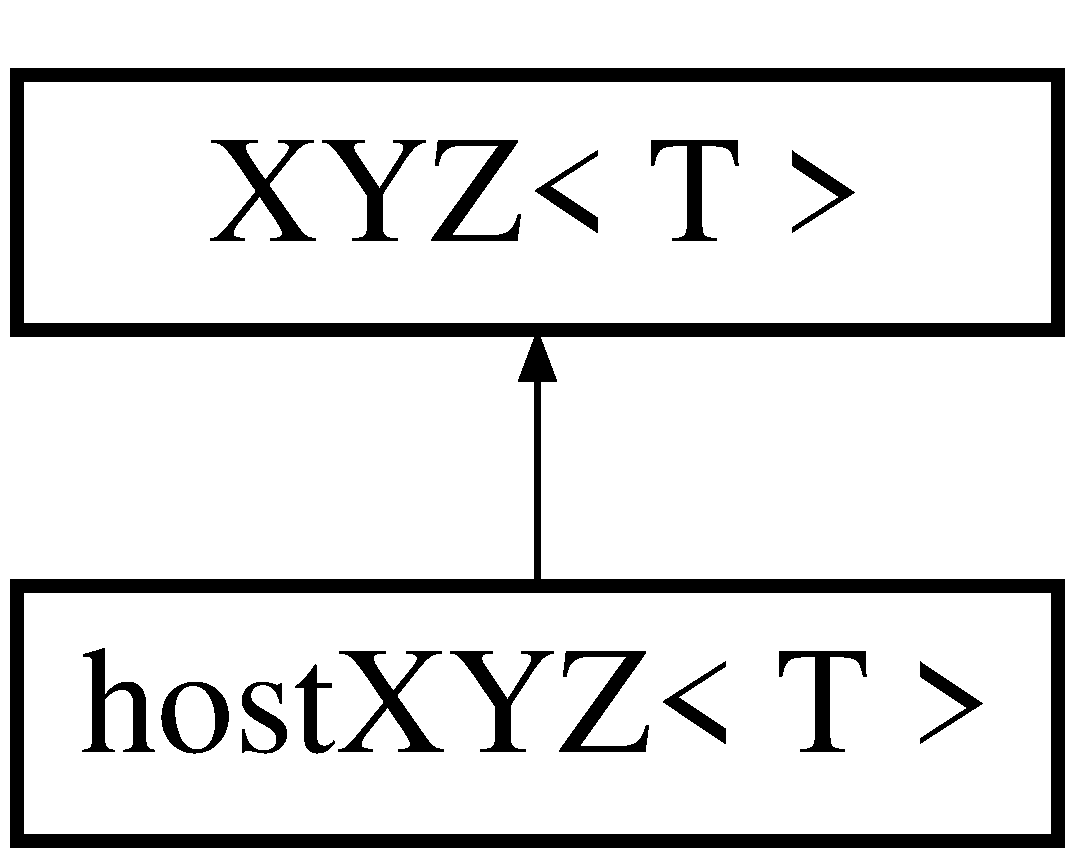
\includegraphics[height=2.000000cm]{classhostXYZ}
\end{center}
\end{figure}
\subsection*{Public Member Functions}
\begin{DoxyCompactItemize}
\item 
\hypertarget{classhostXYZ_aa778fc828bc0c9663e3ba1e594029909}{}\label{classhostXYZ_aa778fc828bc0c9663e3ba1e594029909} 
{\bfseries host\+X\+YZ} (int size, int type=P\+I\+N\+N\+ED)
\item 
\hypertarget{classhostXYZ_a06d4785f9d8f460fcb7d695c62523638}{}\label{classhostXYZ_a06d4785f9d8f460fcb7d695c62523638} 
{\bfseries host\+X\+YZ} (int size, int capacity, T $\ast$x, T $\ast$y, T $\ast$z, int type=P\+I\+N\+N\+ED)
\item 
\hypertarget{classhostXYZ_a77c082148d16bd13d33814c44b698e4c}{}\label{classhostXYZ_a77c082148d16bd13d33814c44b698e4c} 
{\footnotesize template$<$typename P $>$ }\\{\bfseries host\+X\+YZ} (\hyperlink{classcudaXYZ}{cuda\+X\+YZ}$<$ P $>$ \&xyz, int type=P\+I\+N\+N\+ED)
\item 
\hypertarget{classhostXYZ_aa5af59ff12ad0a63441b21a287a84875}{}\label{classhostXYZ_aa5af59ff12ad0a63441b21a287a84875} 
void {\bfseries realloc\+\_\+array} (T $\ast$$\ast$array, int $\ast$capacity, int size, float fac)
\item 
\hypertarget{classhostXYZ_a89f504dfcafda1ea2abccb888227f2db}{}\label{classhostXYZ_a89f504dfcafda1ea2abccb888227f2db} 
void {\bfseries resize\+\_\+array} (T $\ast$$\ast$array, int $\ast$capacity, int size, int new\+\_\+size, float fac)
\item 
\hypertarget{classhostXYZ_af5974c831a3548b39df8528fb4c65e6f}{}\label{classhostXYZ_af5974c831a3548b39df8528fb4c65e6f} 
{\footnotesize template$<$typename P $>$ }\\void {\bfseries set\+\_\+data} (\hyperlink{classcudaXYZ}{cuda\+X\+YZ}$<$ P $>$ \&xyz, cuda\+Stream\+\_\+t stream=0)
\item 
\hypertarget{classhostXYZ_ad0d6cd06fc015dd552a6aae5c520ea73}{}\label{classhostXYZ_ad0d6cd06fc015dd552a6aae5c520ea73} 
{\footnotesize template$<$typename P $>$ }\\void {\bfseries set\+\_\+data\+\_\+sync} (\hyperlink{classcudaXYZ}{cuda\+X\+YZ}$<$ P $>$ \&xyz)
\item 
\hypertarget{classhostXYZ_a27bbb0044ea8c704e872be2b6ea8af6b}{}\label{classhostXYZ_a27bbb0044ea8c704e872be2b6ea8af6b} 
{\footnotesize template$<$typename P $>$ }\\void {\bfseries set\+\_\+data\+\_\+sync} (const int n, \hyperlink{classcudaXYZ}{cuda\+X\+YZ}$<$ P $>$ \&xyz)
\item 
\hypertarget{classhostXYZ_ac4f8f8c54df48574db452735886f8592}{}\label{classhostXYZ_ac4f8f8c54df48574db452735886f8592} 
void {\bfseries set\+\_\+data\+\_\+sync} (const int size, const T $\ast$d\+\_\+x, const T $\ast$d\+\_\+y, const T $\ast$d\+\_\+z)
\item 
\hypertarget{classhostXYZ_aa08825ac00e48ef6b170be03cfe4fcd1}{}\label{classhostXYZ_aa08825ac00e48ef6b170be03cfe4fcd1} 
void {\bfseries set\+\_\+data\+\_\+fromhost} (const int size, const T $\ast$h\+\_\+x, const T $\ast$h\+\_\+y, const T $\ast$h\+\_\+z)
\item 
\hypertarget{classhostXYZ_a91c22d6ee28e2db05a3d9884a9e0bd8b}{}\label{classhostXYZ_a91c22d6ee28e2db05a3d9884a9e0bd8b} 
void {\bfseries get\+\_\+host\+\_\+xyz} (T $\ast$\&hx, T $\ast$\&hy, T $\ast$\&hz)
\item 
\hypertarget{classhostXYZ_afab68d59cabec83d9cbed04614ae718b}{}\label{classhostXYZ_afab68d59cabec83d9cbed04614ae718b} 
void {\bfseries release\+\_\+host\+\_\+xyz} (T $\ast$\&hx, T $\ast$\&hy, T $\ast$\&hz)
\end{DoxyCompactItemize}
\subsection*{Additional Inherited Members}


The documentation for this class was generated from the following files\+:\begin{DoxyCompactItemize}
\item 
/u/samar/\+Documents/git/chcuda/include/cuda\+X\+Y\+Z.\+h\item 
/u/samar/\+Documents/git/chcuda/include/host\+X\+Y\+Z.\+h\end{DoxyCompactItemize}

\hypertarget{structientry__t}{}\section{ientry\+\_\+t Struct Reference}
\label{structientry__t}\index{ientry\+\_\+t@{ientry\+\_\+t}}
\subsection*{Public Attributes}
\begin{DoxyCompactItemize}
\item 
\hypertarget{structientry__t_acf6f06c51e58b2511ff15a1fe57be1fd}{}\label{structientry__t_acf6f06c51e58b2511ff15a1fe57be1fd} 
int {\bfseries iatom\+Start}
\item 
\hypertarget{structientry__t_a379a46e5f7973bd653cea1096f8d979d}{}\label{structientry__t_a379a46e5f7973bd653cea1096f8d979d} 
int {\bfseries ish}
\item 
\hypertarget{structientry__t_a49b14ca044df9ef7fa7251c025a1d1a8}{}\label{structientry__t_a49b14ca044df9ef7fa7251c025a1d1a8} 
int {\bfseries tile\+Start}
\item 
\hypertarget{structientry__t_a770eaa48237b0ac89dd751d29b11e3f6}{}\label{structientry__t_a770eaa48237b0ac89dd751d29b11e3f6} 
int {\bfseries tile\+End}
\end{DoxyCompactItemize}


The documentation for this struct was generated from the following file\+:\begin{DoxyCompactItemize}
\item 
/u/samar/\+Documents/git/chcuda/include/Cuda\+Neighbor\+List\+Build.\+h\end{DoxyCompactItemize}

\hypertarget{structkeyval__t}{}\section{keyval\+\_\+t Struct Reference}
\label{structkeyval__t}\index{keyval\+\_\+t@{keyval\+\_\+t}}
\subsection*{Public Attributes}
\begin{DoxyCompactItemize}
\item 
\hypertarget{structkeyval__t_aa4c1b766401aad398453c07c3c5fe525}{}\label{structkeyval__t_aa4c1b766401aad398453c07c3c5fe525} 
\begin{tabbing}
xx\=xx\=xx\=xx\=xx\=xx\=xx\=xx\=xx\=\kill
union \{\\
\>float {\bfseries key}\\
\>int {\bfseries ind}\\
\}; \\

\end{tabbing}\item 
\hypertarget{structkeyval__t_a5c14a58a275bf5124f483e6e195c9736}{}\label{structkeyval__t_a5c14a58a275bf5124f483e6e195c9736} 
int {\bfseries val}
\end{DoxyCompactItemize}


The documentation for this struct was generated from the following file\+:\begin{DoxyCompactItemize}
\item 
/u/samar/\+Documents/git/chcuda/include/Cuda\+Neighbor\+List\+Sort.\+h\end{DoxyCompactItemize}

\hypertarget{classKineticEnergyGraph}{}\section{Kinetic\+Energy\+Graph Class Reference}
\label{classKineticEnergyGraph}\index{Kinetic\+Energy\+Graph@{Kinetic\+Energy\+Graph}}


Create a graph that calculates the kinetic energy.  




{\ttfamily \#include $<$Kinetic\+Energy\+Graph.\+h$>$}

Inheritance diagram for Kinetic\+Energy\+Graph\+:\begin{figure}[H]
\begin{center}
\leavevmode
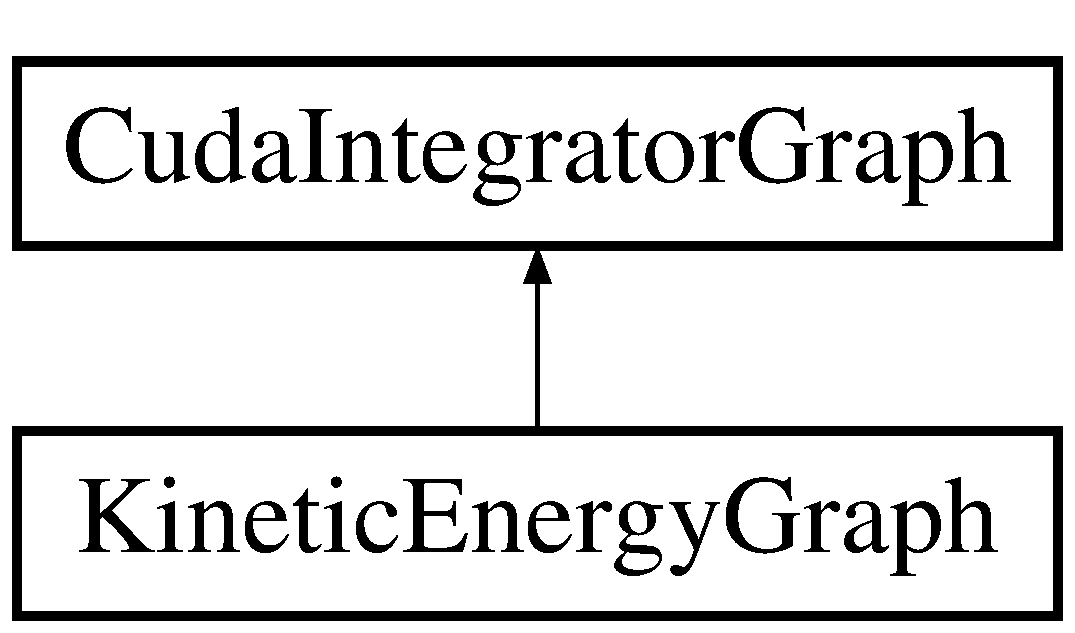
\includegraphics[height=2.000000cm]{classKineticEnergyGraph}
\end{center}
\end{figure}
\subsection*{Public Member Functions}
\begin{DoxyCompactItemize}
\item 
\hyperlink{classKineticEnergyGraph_a5dea5ca46df5e90b2b9ceb5624876113}{Kinetic\+Energy\+Graph} (const double4 $\ast$\+\_\+\+\_\+restrict\+\_\+\+\_\+ vel\+\_\+mass, double $\ast$\+\_\+\+\_\+restrict\+\_\+\+\_\+ total\+\_\+kinetic\+\_\+energy, int num\+Atoms)
\begin{DoxyCompactList}\small\item\em Create a graph that calculate the kinetic energy. \end{DoxyCompactList}\end{DoxyCompactItemize}
\subsection*{Additional Inherited Members}


\subsection{Detailed Description}
Create a graph that calculates the kinetic energy. 



\subsection{Constructor \& Destructor Documentation}
\hypertarget{classKineticEnergyGraph_a5dea5ca46df5e90b2b9ceb5624876113}{}\label{classKineticEnergyGraph_a5dea5ca46df5e90b2b9ceb5624876113} 
\index{Kinetic\+Energy\+Graph@{Kinetic\+Energy\+Graph}!Kinetic\+Energy\+Graph@{Kinetic\+Energy\+Graph}}
\index{Kinetic\+Energy\+Graph@{Kinetic\+Energy\+Graph}!Kinetic\+Energy\+Graph@{Kinetic\+Energy\+Graph}}
\subsubsection{\texorpdfstring{Kinetic\+Energy\+Graph()}{KineticEnergyGraph()}}
{\footnotesize\ttfamily Kinetic\+Energy\+Graph\+::\+Kinetic\+Energy\+Graph (\begin{DoxyParamCaption}\item[{const double4 $\ast$\+\_\+\+\_\+restrict\+\_\+\+\_\+}]{vel\+\_\+mass,  }\item[{double $\ast$\+\_\+\+\_\+restrict\+\_\+\+\_\+}]{total\+\_\+kinetic\+\_\+energy,  }\item[{int}]{num\+Atoms }\end{DoxyParamCaption})}



Create a graph that calculate the kinetic energy. 

All units are SI compatible. 

The documentation for this class was generated from the following file\+:\begin{DoxyCompactItemize}
\item 
/u/samar/\+Documents/git/chcuda/include/\hyperlink{KineticEnergyGraph_8h}{Kinetic\+Energy\+Graph.\+h}\end{DoxyCompactItemize}

\hypertarget{classMatrix3d}{}\section{Matrix3d$<$ T $>$ Class Template Reference}
\label{classMatrix3d}\index{Matrix3d$<$ T $>$@{Matrix3d$<$ T $>$}}
\subsection*{Public Member Functions}
\begin{DoxyCompactItemize}
\item 
\hypertarget{classMatrix3d_ae6ce659b83ce95dbff6e0933fd41261a}{}\label{classMatrix3d_ae6ce659b83ce95dbff6e0933fd41261a} 
{\bfseries Matrix3d} (const int nx, const int ny, const int nz, T $\ast$ext\+\_\+data=N\+U\+LL)
\item 
\hypertarget{classMatrix3d_ab4c7123ef87e71b0f8a4fe2a6b473b6b}{}\label{classMatrix3d_ab4c7123ef87e71b0f8a4fe2a6b473b6b} 
{\bfseries Matrix3d} (const int nx, const int ny, const int nz, const int xsize, const int ysize, const int zsize, T $\ast$ext\+\_\+data=N\+U\+LL)
\item 
\hypertarget{classMatrix3d_a214fa561bafcef5629dc0a5a9162e7b6}{}\label{classMatrix3d_a214fa561bafcef5629dc0a5a9162e7b6} 
{\bfseries Matrix3d} (const int nx, const int ny, const int nz, const char $\ast$filename, T $\ast$ext\+\_\+data=N\+U\+LL)
\item 
\hypertarget{classMatrix3d_a0dc060b22881e4d074c9e43eeaebe657}{}\label{classMatrix3d_a0dc060b22881e4d074c9e43eeaebe657} 
void {\bfseries print\+\_\+info} ()
\item 
\hypertarget{classMatrix3d_a2015e215691333e3ee4fcf321b00ec7b}{}\label{classMatrix3d_a2015e215691333e3ee4fcf321b00ec7b} 
bool {\bfseries compare} (\hyperlink{classMatrix3d}{Matrix3d}$<$ T $>$ $\ast$mat, const double tol, double \&max\+\_\+diff)
\item 
\hypertarget{classMatrix3d_a452265f8fa98fcd7feaec3fcefddb828}{}\label{classMatrix3d_a452265f8fa98fcd7feaec3fcefddb828} 
void {\bfseries transpose\+\_\+xyz\+\_\+yzx\+\_\+host} (int src\+\_\+x0, int src\+\_\+y0, int src\+\_\+z0, int dst\+\_\+x0, int dst\+\_\+y0, int dst\+\_\+z0, int xlen, int ylen, int zlen, \hyperlink{classMatrix3d}{Matrix3d}$<$ T $>$ $\ast$mat)
\item 
\hypertarget{classMatrix3d_aca6bc24fdb30acae66f1f89b434bea6f}{}\label{classMatrix3d_aca6bc24fdb30acae66f1f89b434bea6f} 
void {\bfseries transpose\+\_\+xyz\+\_\+yzx\+\_\+host} (\hyperlink{classMatrix3d}{Matrix3d}$<$ T $>$ $\ast$mat)
\item 
\hypertarget{classMatrix3d_a7eed3fb23f46d42623194e8536d06901}{}\label{classMatrix3d_a7eed3fb23f46d42623194e8536d06901} 
void {\bfseries transpose\+\_\+xyz\+\_\+zxy\+\_\+host} (\hyperlink{classMatrix3d}{Matrix3d}$<$ T $>$ $\ast$mat)
\item 
\hypertarget{classMatrix3d_a970f62c82ece58f5dffcfd16c0c3b6c8}{}\label{classMatrix3d_a970f62c82ece58f5dffcfd16c0c3b6c8} 
void {\bfseries transpose\+\_\+xyz\+\_\+yzx} (\hyperlink{classMatrix3d}{Matrix3d}$<$ T $>$ $\ast$mat)
\item 
\hypertarget{classMatrix3d_ab286179acccc643054d36b67a88aac0a}{}\label{classMatrix3d_ab286179acccc643054d36b67a88aac0a} 
void {\bfseries transpose\+\_\+xyz\+\_\+yzx} (int src\+\_\+x0, int src\+\_\+y0, int src\+\_\+z0, int dst\+\_\+x0, int dst\+\_\+y0, int dst\+\_\+z0, int xlen, int ylen, int zlen, \hyperlink{classMatrix3d}{Matrix3d}$<$ T $>$ $\ast$mat)
\item 
\hypertarget{classMatrix3d_aa89eeeee9451a7fdfa965e7c0a80393e}{}\label{classMatrix3d_aa89eeeee9451a7fdfa965e7c0a80393e} 
void {\bfseries transpose\+\_\+xyz\+\_\+zxy} (\hyperlink{classMatrix3d}{Matrix3d}$<$ T $>$ $\ast$mat)
\item 
\hypertarget{classMatrix3d_a4c0dca7e94a6c276a902523530053d73}{}\label{classMatrix3d_a4c0dca7e94a6c276a902523530053d73} 
void {\bfseries copy\+\_\+host} (int src\+\_\+x0, int src\+\_\+y0, int src\+\_\+z0, int dst\+\_\+x0, int dst\+\_\+y0, int dst\+\_\+z0, int xlen, int ylen, int zlen, \hyperlink{classMatrix3d}{Matrix3d}$<$ T $>$ $\ast$mat)
\item 
\hypertarget{classMatrix3d_a0e186f5e20711362c3f755831d8b73d7}{}\label{classMatrix3d_a0e186f5e20711362c3f755831d8b73d7} 
void {\bfseries copy} (int src\+\_\+x0, int src\+\_\+y0, int src\+\_\+z0, int dst\+\_\+x0, int dst\+\_\+y0, int dst\+\_\+z0, int xlen, int ylen, int zlen, \hyperlink{classMatrix3d}{Matrix3d}$<$ T $>$ $\ast$mat)
\item 
\hypertarget{classMatrix3d_adb5e54dc56bddd5cf6deebda85157516}{}\label{classMatrix3d_adb5e54dc56bddd5cf6deebda85157516} 
void {\bfseries copy} (\hyperlink{classMatrix3d}{Matrix3d}$<$ T $>$ $\ast$mat)
\item 
\hypertarget{classMatrix3d_a87fd2fcb250d8e3b1bbbd0768b9331a5}{}\label{classMatrix3d_a87fd2fcb250d8e3b1bbbd0768b9331a5} 
void {\bfseries print} (const int x0, const int x1, const int y0, const int y1, const int z0, const int z1)
\item 
\hypertarget{classMatrix3d_aea3e3b6e9d02625a4a76a71c3bb677bc}{}\label{classMatrix3d_aea3e3b6e9d02625a4a76a71c3bb677bc} 
void {\bfseries load} (const int x0, const int x1, const int nx, const int y0, const int y1, const int ny, const int z0, const int z1, const int nz, const char $\ast$filename)
\item 
\hypertarget{classMatrix3d_a3d9308431626b0352d5b47603ef61fdc}{}\label{classMatrix3d_a3d9308431626b0352d5b47603ef61fdc} 
void {\bfseries load} (const int nx, const int ny, const int nz, const char $\ast$filename)
\item 
\hypertarget{classMatrix3d_a1c2c8c9fbf3dec15f4a8563ae2dbbbc1}{}\label{classMatrix3d_a1c2c8c9fbf3dec15f4a8563ae2dbbbc1} 
void {\bfseries scale} (const T fac)
\item 
\hypertarget{classMatrix3d_a16373c396a8e6cd5f4766a667308054f}{}\label{classMatrix3d_a16373c396a8e6cd5f4766a667308054f} 
int {\bfseries get\+\_\+nx} ()
\item 
\hypertarget{classMatrix3d_a9408dd026d7fbac4d08302536ad581a1}{}\label{classMatrix3d_a9408dd026d7fbac4d08302536ad581a1} 
int {\bfseries get\+\_\+ny} ()
\item 
\hypertarget{classMatrix3d_aee86893068958f4b1447a720d16f3a21}{}\label{classMatrix3d_aee86893068958f4b1447a720d16f3a21} 
int {\bfseries get\+\_\+nz} ()
\item 
\hypertarget{classMatrix3d_a51f7e43342aa6287fda1ddea32346527}{}\label{classMatrix3d_a51f7e43342aa6287fda1ddea32346527} 
int {\bfseries get\+\_\+xsize} ()
\item 
\hypertarget{classMatrix3d_a1b2d8c8be13cc6ea3f1c8e8822e10afe}{}\label{classMatrix3d_a1b2d8c8be13cc6ea3f1c8e8822e10afe} 
int {\bfseries get\+\_\+ysize} ()
\item 
\hypertarget{classMatrix3d_aaaeab4d3f5cc6af74f82ac7bd42f1886}{}\label{classMatrix3d_aaaeab4d3f5cc6af74f82ac7bd42f1886} 
int {\bfseries get\+\_\+zsize} ()
\end{DoxyCompactItemize}
\subsection*{Public Attributes}
\begin{DoxyCompactItemize}
\item 
\hypertarget{classMatrix3d_accb9a3fa73d931d63d63745ab95d6fbe}{}\label{classMatrix3d_accb9a3fa73d931d63d63745ab95d6fbe} 
T $\ast$ {\bfseries data}
\end{DoxyCompactItemize}
\subsection*{Protected Attributes}
\begin{DoxyCompactItemize}
\item 
\hypertarget{classMatrix3d_a3f51885c4443ba1b49973167bd70ba5a}{}\label{classMatrix3d_a3f51885c4443ba1b49973167bd70ba5a} 
int {\bfseries nx}
\item 
\hypertarget{classMatrix3d_a006c9a3a7ec1ae18e32536a22e13e8fe}{}\label{classMatrix3d_a006c9a3a7ec1ae18e32536a22e13e8fe} 
int {\bfseries ny}
\item 
\hypertarget{classMatrix3d_a066681c25c06add097736316470ee4e2}{}\label{classMatrix3d_a066681c25c06add097736316470ee4e2} 
int {\bfseries nz}
\item 
\hypertarget{classMatrix3d_a7ae88ff46c6e20f95faa1ffc76804c06}{}\label{classMatrix3d_a7ae88ff46c6e20f95faa1ffc76804c06} 
int {\bfseries xsize}
\item 
\hypertarget{classMatrix3d_a42f5e7f9d870544bd8e0d9c3cc41a699}{}\label{classMatrix3d_a42f5e7f9d870544bd8e0d9c3cc41a699} 
int {\bfseries ysize}
\item 
\hypertarget{classMatrix3d_adc57dfb65c173d37208f42f1538c695d}{}\label{classMatrix3d_adc57dfb65c173d37208f42f1538c695d} 
int {\bfseries zsize}
\end{DoxyCompactItemize}


The documentation for this class was generated from the following file\+:\begin{DoxyCompactItemize}
\item 
/u/samar/\+Documents/git/chcuda/include/Matrix3d.\+h\end{DoxyCompactItemize}

\hypertarget{classr123_1_1MicroURNG}{}\section{r123\+:\+:Micro\+U\+R\+NG$<$ C\+B\+R\+NG $>$ Class Template Reference}
\label{classr123_1_1MicroURNG}\index{r123\+::\+Micro\+U\+R\+N\+G$<$ C\+B\+R\+N\+G $>$@{r123\+::\+Micro\+U\+R\+N\+G$<$ C\+B\+R\+N\+G $>$}}


Given a C\+B\+R\+NG whose ctr\+\_\+type has an unsigned integral value\+\_\+type, Micro\+U\+R\+N\+G$<$\+C\+B\+R\+N\+G$>$(c, k) is a type that satisfies the requirements of a C++11 Uniform Random Number Generator.  




{\ttfamily \#include $<$Micro\+U\+R\+N\+G.\+hpp$>$}

\subsection*{Public Types}
\begin{DoxyCompactItemize}
\item 
\hypertarget{classr123_1_1MicroURNG_ab0b3a77c9408dbcb2f9d6b5c67e9c3f7}{}\label{classr123_1_1MicroURNG_ab0b3a77c9408dbcb2f9d6b5c67e9c3f7} 
typedef C\+B\+R\+NG {\bfseries cbrng\+\_\+type}
\item 
\hypertarget{classr123_1_1MicroURNG_a5aba882fd21e4d8f1a445f546e1e4476}{}\label{classr123_1_1MicroURNG_a5aba882fd21e4d8f1a445f546e1e4476} 
typedef cbrng\+\_\+type\+::ctr\+\_\+type {\bfseries ctr\+\_\+type}
\item 
\hypertarget{classr123_1_1MicroURNG_aef90e6157f360434342ad0df4ce5f364}{}\label{classr123_1_1MicroURNG_aef90e6157f360434342ad0df4ce5f364} 
typedef cbrng\+\_\+type\+::key\+\_\+type {\bfseries key\+\_\+type}
\item 
\hypertarget{classr123_1_1MicroURNG_a7e6fd93fec2fe138ee36b401ff376cfc}{}\label{classr123_1_1MicroURNG_a7e6fd93fec2fe138ee36b401ff376cfc} 
typedef cbrng\+\_\+type\+::ukey\+\_\+type {\bfseries ukey\+\_\+type}
\item 
\hypertarget{classr123_1_1MicroURNG_a512957c3e7b3d22741ef0a436b973c2b}{}\label{classr123_1_1MicroURNG_a512957c3e7b3d22741ef0a436b973c2b} 
typedef ctr\+\_\+type\+::value\+\_\+type {\bfseries result\+\_\+type}
\end{DoxyCompactItemize}
\subsection*{Public Member Functions}
\begin{DoxyCompactItemize}
\item 
\hypertarget{classr123_1_1MicroURNG_a82982e0df155e33f0899867f5d7cca53}{}\label{classr123_1_1MicroURNG_a82982e0df155e33f0899867f5d7cca53} 
{\bfseries R123\+\_\+\+S\+T\+A\+T\+I\+C\+\_\+\+A\+S\+S\+E\+RT} (std\+::numeric\+\_\+limits$<$ result\+\_\+type $>$\+::digits $>$=B\+I\+TS, \char`\"{}The result\+\_\+type must have at least 32 bits\char`\"{})
\item 
\hypertarget{classr123_1_1MicroURNG_a64cd4d33b4cab5d3d9c556db68407b77}{}\label{classr123_1_1MicroURNG_a64cd4d33b4cab5d3d9c556db68407b77} 
result\+\_\+type {\bfseries operator()} ()
\item 
\hypertarget{classr123_1_1MicroURNG_a19afb80312c370e1670bf8afc73d802e}{}\label{classr123_1_1MicroURNG_a19afb80312c370e1670bf8afc73d802e} 
{\bfseries Micro\+U\+R\+NG} (cbrng\+\_\+type \+\_\+b, ctr\+\_\+type \+\_\+c0, ukey\+\_\+type \+\_\+uk)
\item 
\hypertarget{classr123_1_1MicroURNG_a7ecf43819bc96804892a78c6715f587b}{}\label{classr123_1_1MicroURNG_a7ecf43819bc96804892a78c6715f587b} 
{\bfseries Micro\+U\+R\+NG} (ctr\+\_\+type \+\_\+c0, ukey\+\_\+type \+\_\+uk)
\item 
\hypertarget{classr123_1_1MicroURNG_a1729ed31ddf93325fee2e5413c3d3817}{}\label{classr123_1_1MicroURNG_a1729ed31ddf93325fee2e5413c3d3817} 
const ctr\+\_\+type \& {\bfseries counter} () const
\item 
\hypertarget{classr123_1_1MicroURNG_add2f214254ddc2291e3b2c8b5dbe791a}{}\label{classr123_1_1MicroURNG_add2f214254ddc2291e3b2c8b5dbe791a} 
void {\bfseries reset} (ctr\+\_\+type \+\_\+c0, ukey\+\_\+type \+\_\+uk)
\end{DoxyCompactItemize}
\subsection*{Static Public Member Functions}
\begin{DoxyCompactItemize}
\item 
\hypertarget{classr123_1_1MicroURNG_aa05c857c01053cf9185406d69757b101}{}\label{classr123_1_1MicroURNG_aa05c857c01053cf9185406d69757b101} 
static R123\+\_\+\+C\+O\+N\+S\+T\+E\+X\+PR result\+\_\+type min {\bfseries R123\+\_\+\+N\+O\+\_\+\+M\+A\+C\+R\+O\+\_\+\+S\+U\+B\+ST} ()
\item 
\hypertarget{classr123_1_1MicroURNG_a3af623b6366d6e848d67d72e4b0f363c}{}\label{classr123_1_1MicroURNG_a3af623b6366d6e848d67d72e4b0f363c} 
static R123\+\_\+\+C\+O\+N\+S\+T\+E\+X\+PR result\+\_\+type max {\bfseries R123\+\_\+\+N\+O\+\_\+\+M\+A\+C\+R\+O\+\_\+\+S\+U\+B\+ST} ()
\end{DoxyCompactItemize}
\subsection*{Static Public Attributes}
\begin{DoxyCompactItemize}
\item 
\hypertarget{classr123_1_1MicroURNG_ac55cddda8fe0808f922f39beee587b27}{}\label{classr123_1_1MicroURNG_ac55cddda8fe0808f922f39beee587b27} 
static const int {\bfseries B\+I\+TS} = 32
\item 
\hypertarget{classr123_1_1MicroURNG_a1f2787f136a8a807d14eab8cb1ca8c14}{}\label{classr123_1_1MicroURNG_a1f2787f136a8a807d14eab8cb1ca8c14} 
static const result\+\_\+type {\bfseries \+\_\+\+Min} = 0
\item 
\hypertarget{classr123_1_1MicroURNG_a4faecd7ab54c7678ee66c413bb984bf0}{}\label{classr123_1_1MicroURNG_a4faecd7ab54c7678ee66c413bb984bf0} 
static const result\+\_\+type {\bfseries \+\_\+\+Max} = $\sim$((result\+\_\+type)0)
\end{DoxyCompactItemize}


\subsection{Detailed Description}
\subsubsection*{template$<$typename C\+B\+R\+NG$>$\newline
class r123\+::\+Micro\+U\+R\+N\+G$<$ C\+B\+R\+N\+G $>$}

Given a C\+B\+R\+NG whose ctr\+\_\+type has an unsigned integral value\+\_\+type, Micro\+U\+R\+N\+G$<$\+C\+B\+R\+N\+G$>$(c, k) is a type that satisfies the requirements of a C++11 Uniform Random Number Generator. 

The intended purpose is for a \hyperlink{classr123_1_1MicroURNG}{Micro\+U\+R\+NG} to be passed as an argument to a C++11 Distribution, e.\+g., std\+::normal\+\_\+distribution. See examples/\+Micro\+U\+R\+N\+G.\+cpp.

The \hyperlink{classr123_1_1MicroURNG}{Micro\+U\+R\+NG} functor has a period of \char`\"{}only\char`\"{}

ctr\+\_\+type.\+size()$\ast$2$^\wedge$32,

after which it will silently repeat.

The high 32 bits of the highest word in the counter c, passed to the constructor must be zero. \hyperlink{classr123_1_1MicroURNG}{Micro\+U\+R\+NG} uses these bits to \char`\"{}count\char`\"{}.

Older versions of the library permitted a second template parameter by which the caller could control the number of bits devoted to the U\+R\+NG\textquotesingle{}s internal counter. This flexibility has been disabled because U\+R\+N\+Gs created with different numbers of counter bits could, conceivably \char`\"{}collide\char`\"{}.


\begin{DoxyCode}
\textcolor{keyword}{typedef} ?someCBRNG? RNG;
RNG::ctr\_type c = ...; \textcolor{comment}{// under application control}
RNG::key\_type k = ...; \textcolor{comment}{// }
std::normal\_distribution<float> nd;
MicroURNG<RNG> urng(c, k);
\textcolor{keywordflow}{for}(???)\{
  ...
  nd(urng);  \textcolor{comment}{// may be called several hundred times with BITS=10}
  ...
\}
\end{DoxyCode}
 

The documentation for this class was generated from the following file\+:\begin{DoxyCompactItemize}
\item 
/u/samar/\+Documents/git/chcuda/include/\+Random123/Micro\+U\+R\+N\+G.\+hpp\end{DoxyCompactItemize}

\hypertarget{structNlistParam__t}{}\section{Nlist\+Param\+\_\+t Struct Reference}
\label{structNlistParam__t}\index{Nlist\+Param\+\_\+t@{Nlist\+Param\+\_\+t}}
\subsection*{Public Attributes}
\begin{DoxyCompactItemize}
\item 
\hypertarget{structNlistParam__t_ab78706c9bdb3af53d24fd50f883c1546}{}\label{structNlistParam__t_ab78706c9bdb3af53d24fd50f883c1546} 
int {\bfseries imx\+\_\+lo}
\item 
\hypertarget{structNlistParam__t_a130bf747b9187d966840877eef55b913}{}\label{structNlistParam__t_a130bf747b9187d966840877eef55b913} 
int {\bfseries imx\+\_\+hi}
\item 
\hypertarget{structNlistParam__t_ae36497da13c5d2704f16e0a31fbf0dfd}{}\label{structNlistParam__t_ae36497da13c5d2704f16e0a31fbf0dfd} 
int {\bfseries imy\+\_\+lo}
\item 
\hypertarget{structNlistParam__t_a045160b343cd0a982bdb4e167536f500}{}\label{structNlistParam__t_a045160b343cd0a982bdb4e167536f500} 
int {\bfseries imy\+\_\+hi}
\item 
\hypertarget{structNlistParam__t_a153e766348447e178460a4f6cc36f97d}{}\label{structNlistParam__t_a153e766348447e178460a4f6cc36f97d} 
int {\bfseries imz\+\_\+lo}
\item 
\hypertarget{structNlistParam__t_a111e667909fc5eb69c3b4b9166aba9ed}{}\label{structNlistParam__t_a111e667909fc5eb69c3b4b9166aba9ed} 
int {\bfseries imz\+\_\+hi}
\item 
\hypertarget{structNlistParam__t_a6a6cfb049e7452fcd591c268f038aa49}{}\label{structNlistParam__t_a6a6cfb049e7452fcd591c268f038aa49} 
int {\bfseries ncell}
\item 
\hypertarget{structNlistParam__t_a38820ee7ed32e7238e6672f53f3b152f}{}\label{structNlistParam__t_a38820ee7ed32e7238e6672f53f3b152f} 
int {\bfseries n\+\_\+ientry}
\item 
\hypertarget{structNlistParam__t_a0af748e52cee437bb345cb0d37a1890c}{}\label{structNlistParam__t_a0af748e52cee437bb345cb0d37a1890c} 
int {\bfseries n\+\_\+tile}
\item 
\hypertarget{structNlistParam__t_af8004cb95328ab090b3081132aecc433}{}\label{structNlistParam__t_af8004cb95328ab090b3081132aecc433} 
int {\bfseries nexcl}
\end{DoxyCompactItemize}


The documentation for this struct was generated from the following file\+:\begin{DoxyCompactItemize}
\item 
/u/samar/\+Documents/git/chcuda/include/Cuda\+Neighbor\+List\+Struct.\+h\end{DoxyCompactItemize}

\hypertarget{structnum__excl}{}\section{num\+\_\+excl$<$ tilesize $>$ Struct Template Reference}
\label{structnum__excl}\index{num\+\_\+excl$<$ tilesize $>$@{num\+\_\+excl$<$ tilesize $>$}}
\subsection*{Static Public Attributes}
\begin{DoxyCompactItemize}
\item 
\hypertarget{structnum__excl_abeb7d90de252d629164350568920ac58}{}\label{structnum__excl_abeb7d90de252d629164350568920ac58} 
static const int {\bfseries val} = ((tilesize $\ast$ tilesize -\/ 1) / 32 + 1)
\end{DoxyCompactItemize}


The documentation for this struct was generated from the following file\+:\begin{DoxyCompactItemize}
\item 
/u/samar/\+Documents/git/chcuda/include/Cuda\+Neighbor\+List\+Build.\+h\end{DoxyCompactItemize}

\hypertarget{classPressureGroupMomentumUpdate}{}\section{Pressure\+Group\+Momentum\+Update Class Reference}
\label{classPressureGroupMomentumUpdate}\index{Pressure\+Group\+Momentum\+Update@{Pressure\+Group\+Momentum\+Update}}


Create a graph that gets the net force on each pressure group and calc the new momentum.  




{\ttfamily \#include $<$Pressure\+Group\+Momentum\+Update.\+h$>$}

Inheritance diagram for Pressure\+Group\+Momentum\+Update\+:\begin{figure}[H]
\begin{center}
\leavevmode
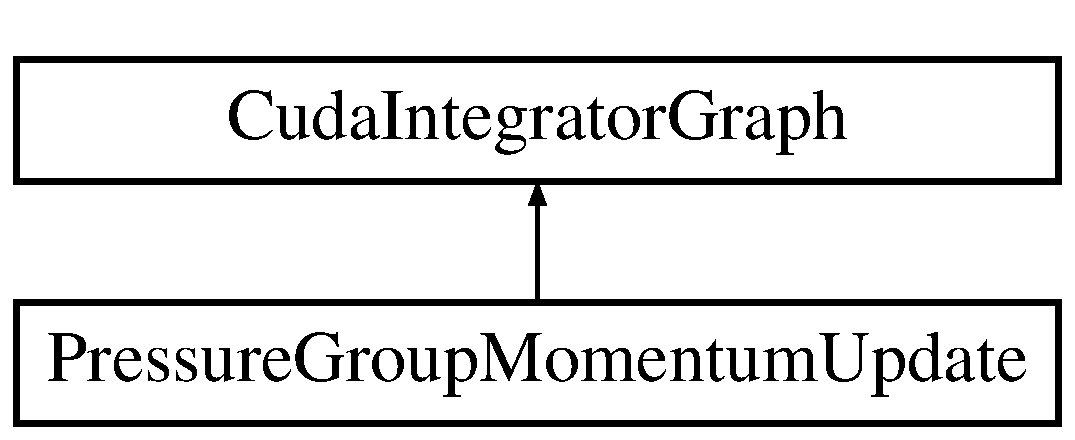
\includegraphics[height=2.000000cm]{classPressureGroupMomentumUpdate}
\end{center}
\end{figure}
\subsection*{Public Member Functions}
\begin{DoxyCompactItemize}
\item 
\hyperlink{classPressureGroupMomentumUpdate_a2bfd6839085a1c51d0e2354dd1626763}{Pressure\+Group\+Momentum\+Update} (const double $\ast$\+\_\+\+\_\+restrict\+\_\+\+\_\+ fx, const double $\ast$\+\_\+\+\_\+restrict\+\_\+\+\_\+ fy, const double $\ast$\+\_\+\+\_\+restrict\+\_\+\+\_\+ fz, const double4 $\ast$old\+\_\+momentum\+\_\+invmass, double4 $\ast$new\+\_\+momentum\+\_\+invmass, const \hyperlink{structAtomIdList__t}{Atom\+Id\+List\+\_\+t} $\ast$\+\_\+\+\_\+restrict\+\_\+\+\_\+ group\+\_\+atom\+\_\+ids, double timestep, int num\+Groups)
\begin{DoxyCompactList}\small\item\em Create a graph that gets the net force on each pressure group and updates the group net momentum. \end{DoxyCompactList}\item 
\hyperlink{classPressureGroupMomentumUpdate_aa41078d9fadcd907d39c9ba18b3920ca}{$\sim$\+Pressure\+Group\+Momentum\+Update} ()
\begin{DoxyCompactList}\small\item\em Destroy the graph, its nodes, and free internal memory. \end{DoxyCompactList}\end{DoxyCompactItemize}
\subsection*{Additional Inherited Members}


\subsection{Detailed Description}
Create a graph that gets the net force on each pressure group and calc the new momentum. 



\subsection{Constructor \& Destructor Documentation}
\hypertarget{classPressureGroupMomentumUpdate_a2bfd6839085a1c51d0e2354dd1626763}{}\label{classPressureGroupMomentumUpdate_a2bfd6839085a1c51d0e2354dd1626763} 
\index{Pressure\+Group\+Momentum\+Update@{Pressure\+Group\+Momentum\+Update}!Pressure\+Group\+Momentum\+Update@{Pressure\+Group\+Momentum\+Update}}
\index{Pressure\+Group\+Momentum\+Update@{Pressure\+Group\+Momentum\+Update}!Pressure\+Group\+Momentum\+Update@{Pressure\+Group\+Momentum\+Update}}
\subsubsection{\texorpdfstring{Pressure\+Group\+Momentum\+Update()}{PressureGroupMomentumUpdate()}}
{\footnotesize\ttfamily Pressure\+Group\+Momentum\+Update\+::\+Pressure\+Group\+Momentum\+Update (\begin{DoxyParamCaption}\item[{const double $\ast$\+\_\+\+\_\+restrict\+\_\+\+\_\+}]{fx,  }\item[{const double $\ast$\+\_\+\+\_\+restrict\+\_\+\+\_\+}]{fy,  }\item[{const double $\ast$\+\_\+\+\_\+restrict\+\_\+\+\_\+}]{fz,  }\item[{const double4 $\ast$}]{old\+\_\+momentum\+\_\+invmass,  }\item[{double4 $\ast$}]{new\+\_\+momentum\+\_\+invmass,  }\item[{const \hyperlink{structAtomIdList__t}{Atom\+Id\+List\+\_\+t} $\ast$\+\_\+\+\_\+restrict\+\_\+\+\_\+}]{group\+\_\+atom\+\_\+ids,  }\item[{double}]{timestep,  }\item[{int}]{num\+Groups }\end{DoxyParamCaption})}



Create a graph that gets the net force on each pressure group and updates the group net momentum. 

All units are SI compatible, defining constants (planks constant, speed of light, charge of electron..., and such) may be different. 
\begin{DoxyParams}{Parameters}
{\em fx,fy,fz} & the device pointers to the array of atom forces. These must be in the same order as the atom ids. \\
\hline
{\em old\+\_\+momentum\+\_\+invmass} & The device pointer to the array of previous net momentums, and the inverse of the net masses, num\+Groups long. \\
\hline
{\em new\+\_\+momentum\+\_\+invmass} & \mbox{[}out\mbox{]} The device pointer to the array of new net momentums, and the inverse of the net masses, num\+Groups long. \\
\hline
{\em group\+\_\+atom\+\_\+ids} & The device pointer to the array of what atoms are in each pressure group. \\
\hline
{\em timestep} & Time step, how long the force should be applied. \\
\hline
{\em num\+Groups} & Number of groups. \\
\hline
\end{DoxyParams}
\hypertarget{classPressureGroupMomentumUpdate_aa41078d9fadcd907d39c9ba18b3920ca}{}\label{classPressureGroupMomentumUpdate_aa41078d9fadcd907d39c9ba18b3920ca} 
\index{Pressure\+Group\+Momentum\+Update@{Pressure\+Group\+Momentum\+Update}!````~Pressure\+Group\+Momentum\+Update@{$\sim$\+Pressure\+Group\+Momentum\+Update}}
\index{````~Pressure\+Group\+Momentum\+Update@{$\sim$\+Pressure\+Group\+Momentum\+Update}!Pressure\+Group\+Momentum\+Update@{Pressure\+Group\+Momentum\+Update}}
\subsubsection{\texorpdfstring{$\sim$\+Pressure\+Group\+Momentum\+Update()}{~PressureGroupMomentumUpdate()}}
{\footnotesize\ttfamily Pressure\+Group\+Momentum\+Update\+::$\sim$\+Pressure\+Group\+Momentum\+Update (\begin{DoxyParamCaption}{ }\end{DoxyParamCaption})}



Destroy the graph, its nodes, and free internal memory. 



The documentation for this class was generated from the following file\+:\begin{DoxyCompactItemize}
\item 
/u/samar/\+Documents/git/chcuda/include/\hyperlink{PressureGroupMomentumUpdate_8h}{Pressure\+Group\+Momentum\+Update.\+h}\end{DoxyCompactItemize}

\hypertarget{classPressureGroupScaleDrift}{}\section{Pressure\+Group\+Scale\+Drift Class Reference}
\label{classPressureGroupScaleDrift}\index{Pressure\+Group\+Scale\+Drift@{Pressure\+Group\+Scale\+Drift}}


Create a graph that calculates the new pressure group center positions and momentums with scaling.  




{\ttfamily \#include $<$Pressure\+Group\+Scale\+Drift.\+h$>$}

Inheritance diagram for Pressure\+Group\+Scale\+Drift\+:\begin{figure}[H]
\begin{center}
\leavevmode
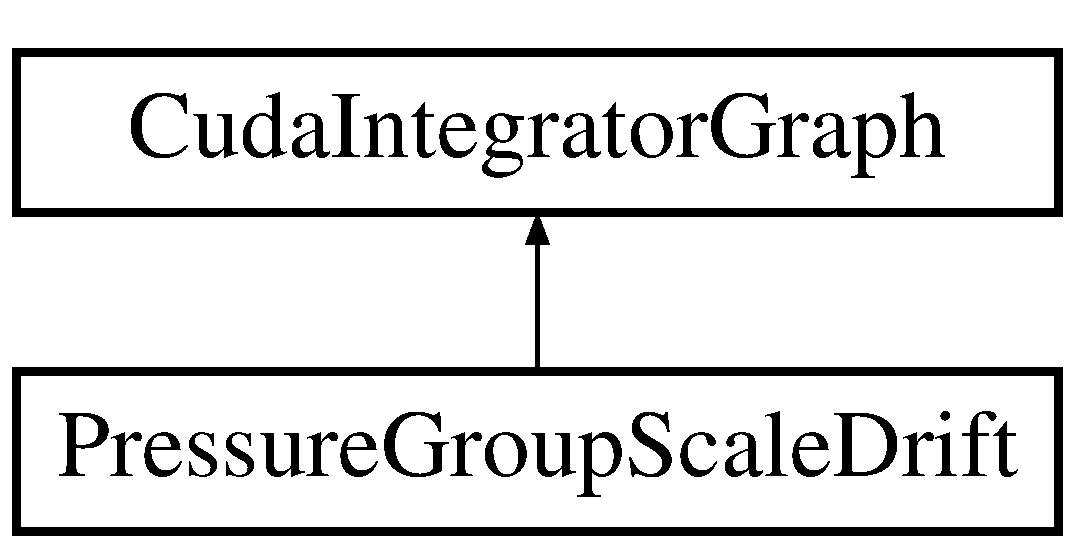
\includegraphics[height=2.000000cm]{classPressureGroupScaleDrift}
\end{center}
\end{figure}
\subsection*{Public Member Functions}
\begin{DoxyCompactItemize}
\item 
\hyperlink{classPressureGroupScaleDrift_a8cf59e5fe7570632084b614bd2000790}{Pressure\+Group\+Scale\+Drift} (const double3 $\ast$\+\_\+\+\_\+restrict\+\_\+\+\_\+ momentum\+\_\+scale, const double3 $\ast$\+\_\+\+\_\+restrict\+\_\+\+\_\+ momentum\+\_\+prescale, const double3 $\ast$\+\_\+\+\_\+restrict\+\_\+\+\_\+ position\+\_\+prescale, const double4 $\ast$old\+\_\+momentum\+\_\+invmass, const double4 $\ast$old\+\_\+xyzq, double4 $\ast$new\+\_\+momentum\+\_\+invmass, double4 $\ast$new\+\_\+xyzq, double timestep, int num)
\begin{DoxyCompactList}\small\item\em Create a graph to move positions and scale pressure group centers of mass and momentum. \end{DoxyCompactList}\end{DoxyCompactItemize}
\subsection*{Additional Inherited Members}


\subsection{Detailed Description}
Create a graph that calculates the new pressure group center positions and momentums with scaling. 

new\+\_\+momentum= old\+\_\+momentum$\ast$momentum\+\_\+scale new\+\_\+xyz= old\+\_\+xyz$\ast$position\+\_\+prescale+timestep$\ast$momentum$\ast$invmass$\ast$momentum\+\_\+prescale 

\subsection{Constructor \& Destructor Documentation}
\hypertarget{classPressureGroupScaleDrift_a8cf59e5fe7570632084b614bd2000790}{}\label{classPressureGroupScaleDrift_a8cf59e5fe7570632084b614bd2000790} 
\index{Pressure\+Group\+Scale\+Drift@{Pressure\+Group\+Scale\+Drift}!Pressure\+Group\+Scale\+Drift@{Pressure\+Group\+Scale\+Drift}}
\index{Pressure\+Group\+Scale\+Drift@{Pressure\+Group\+Scale\+Drift}!Pressure\+Group\+Scale\+Drift@{Pressure\+Group\+Scale\+Drift}}
\subsubsection{\texorpdfstring{Pressure\+Group\+Scale\+Drift()}{PressureGroupScaleDrift()}}
{\footnotesize\ttfamily Pressure\+Group\+Scale\+Drift\+::\+Pressure\+Group\+Scale\+Drift (\begin{DoxyParamCaption}\item[{const double3 $\ast$\+\_\+\+\_\+restrict\+\_\+\+\_\+}]{momentum\+\_\+scale,  }\item[{const double3 $\ast$\+\_\+\+\_\+restrict\+\_\+\+\_\+}]{momentum\+\_\+prescale,  }\item[{const double3 $\ast$\+\_\+\+\_\+restrict\+\_\+\+\_\+}]{position\+\_\+prescale,  }\item[{const double4 $\ast$}]{old\+\_\+momentum\+\_\+invmass,  }\item[{const double4 $\ast$}]{old\+\_\+xyzq,  }\item[{double4 $\ast$}]{new\+\_\+momentum\+\_\+invmass,  }\item[{double4 $\ast$}]{new\+\_\+xyzq,  }\item[{double}]{timestep,  }\item[{int}]{num }\end{DoxyParamCaption})}



Create a graph to move positions and scale pressure group centers of mass and momentum. 


\begin{DoxyParams}{Parameters}
{\em momentum\+\_\+scale} & Device Pointer to total scaling of momentum. \\
\hline
{\em momentum\+\_\+prescale} & Device pointer to momentum scaling for position update. \\
\hline
{\em position\+\_\+prescale} & Device pointer to position scaling before moving. \\
\hline
{\em old\+\_\+momentum\+\_\+invmass} & Device pointer to array of momentums and inverse masses. \\
\hline
{\em old\+\_\+xyzq} & Device pointer to array of positions. \\
\hline
{\em new\+\_\+momentum\+\_\+invmass} & Device pointer to array of new momentums, and invers masses. \\
\hline
{\em new\+\_\+xyzq} & Device pointer to array of new positions. \\
\hline
{\em timestep} & time step. \\
\hline
{\em num} & number of elements in the arrays. \\
\hline
\end{DoxyParams}


The documentation for this class was generated from the following file\+:\begin{DoxyCompactItemize}
\item 
/u/samar/\+Documents/git/chcuda/include/\hyperlink{PressureGroupScaleDrift_8h}{Pressure\+Group\+Scale\+Drift.\+h}\end{DoxyCompactItemize}

\hypertarget{classPressureGroupVirialGraph}{}\section{Pressure\+Group\+Virial\+Graph Class Reference}
\label{classPressureGroupVirialGraph}\index{Pressure\+Group\+Virial\+Graph@{Pressure\+Group\+Virial\+Graph}}


Creates a graph that calculates the virial correction for pressure groups.  




{\ttfamily \#include $<$Pressure\+Group\+Virial.\+h$>$}

Inheritance diagram for Pressure\+Group\+Virial\+Graph\+:\begin{figure}[H]
\begin{center}
\leavevmode
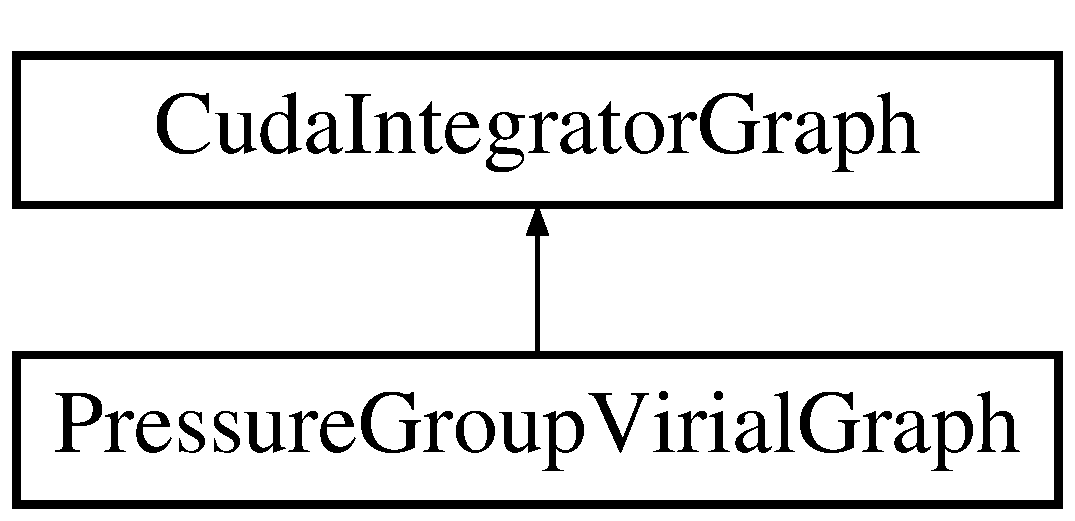
\includegraphics[height=2.000000cm]{classPressureGroupVirialGraph}
\end{center}
\end{figure}
\subsection*{Public Member Functions}
\begin{DoxyCompactItemize}
\item 
\hyperlink{classPressureGroupVirialGraph_ae7ff1b34d814a6c977a50430167f4304}{Pressure\+Group\+Virial\+Graph} (const double $\ast$\+\_\+\+\_\+restrict\+\_\+\+\_\+ forcex, const double $\ast$\+\_\+\+\_\+restrict\+\_\+\+\_\+ forcey, const double $\ast$\+\_\+\+\_\+restrict\+\_\+\+\_\+ forcez, const double $\ast$\+\_\+\+\_\+restrict\+\_\+\+\_\+ relative\+\_\+coordsx, const double $\ast$\+\_\+\+\_\+restrict\+\_\+\+\_\+ relative\+\_\+coordsy, const double $\ast$\+\_\+\+\_\+restrict\+\_\+\+\_\+ relative\+\_\+coordsz, int num\+Atoms, double3 $\ast$\+\_\+\+\_\+restrict\+\_\+\+\_\+ virial)
\begin{DoxyCompactList}\small\item\em Create a graph that calculates and accumulates the pressure group internal virial. \end{DoxyCompactList}\item 
\hyperlink{classPressureGroupVirialGraph_a7f8e55580a547bf7e671cdb4fb590cd9}{$\sim$\+Pressure\+Group\+Virial\+Graph} ()
\begin{DoxyCompactList}\small\item\em Destroy the graph, its nodes, and free internal memory. \end{DoxyCompactList}\item 
\hyperlink{classPressureGroupVirialGraph_acc008fb3d4ecd0443509fb21c92ba592}{Pressure\+Group\+Virial\+Graph} (const double $\ast$\+\_\+\+\_\+restrict\+\_\+\+\_\+ fx, const double $\ast$\+\_\+\+\_\+restrict\+\_\+\+\_\+ fy, const double $\ast$\+\_\+\+\_\+restrict\+\_\+\+\_\+ fz, const double $\ast$\+\_\+\+\_\+restrict\+\_\+\+\_\+ x, const double $\ast$\+\_\+\+\_\+restrict\+\_\+\+\_\+ y, const double $\ast$\+\_\+\+\_\+restrict\+\_\+\+\_\+ z, int num\+Atoms, double3 $\ast$\+\_\+\+\_\+restrict\+\_\+\+\_\+ virial)
\begin{DoxyCompactList}\small\item\em Create a graph that calculates and accumulates the pressure group internal virial. \end{DoxyCompactList}\item 
\hyperlink{classPressureGroupVirialGraph_a7f8e55580a547bf7e671cdb4fb590cd9}{$\sim$\+Pressure\+Group\+Virial\+Graph} ()
\begin{DoxyCompactList}\small\item\em Destroy the graph, its nodes, and free internal memory. \end{DoxyCompactList}\end{DoxyCompactItemize}
\subsection*{Additional Inherited Members}


\subsection{Detailed Description}
Creates a graph that calculates the virial correction for pressure groups. 

\subsection{Constructor \& Destructor Documentation}
\hypertarget{classPressureGroupVirialGraph_ae7ff1b34d814a6c977a50430167f4304}{}\label{classPressureGroupVirialGraph_ae7ff1b34d814a6c977a50430167f4304} 
\index{Pressure\+Group\+Virial\+Graph@{Pressure\+Group\+Virial\+Graph}!Pressure\+Group\+Virial\+Graph@{Pressure\+Group\+Virial\+Graph}}
\index{Pressure\+Group\+Virial\+Graph@{Pressure\+Group\+Virial\+Graph}!Pressure\+Group\+Virial\+Graph@{Pressure\+Group\+Virial\+Graph}}
\subsubsection{\texorpdfstring{Pressure\+Group\+Virial\+Graph()}{PressureGroupVirialGraph()}\hspace{0.1cm}{\footnotesize\ttfamily [1/2]}}
{\footnotesize\ttfamily Pressure\+Group\+Virial\+Graph\+::\+Pressure\+Group\+Virial\+Graph (\begin{DoxyParamCaption}\item[{const double $\ast$\+\_\+\+\_\+restrict\+\_\+\+\_\+}]{forcex,  }\item[{const double $\ast$\+\_\+\+\_\+restrict\+\_\+\+\_\+}]{forcey,  }\item[{const double $\ast$\+\_\+\+\_\+restrict\+\_\+\+\_\+}]{forcez,  }\item[{const double $\ast$\+\_\+\+\_\+restrict\+\_\+\+\_\+}]{relative\+\_\+coordsx,  }\item[{const double $\ast$\+\_\+\+\_\+restrict\+\_\+\+\_\+}]{relative\+\_\+coordsy,  }\item[{const double $\ast$\+\_\+\+\_\+restrict\+\_\+\+\_\+}]{relative\+\_\+coordsz,  }\item[{int}]{num\+Atoms,  }\item[{double3 $\ast$\+\_\+\+\_\+restrict\+\_\+\+\_\+}]{virial }\end{DoxyParamCaption})}



Create a graph that calculates and accumulates the pressure group internal virial. 


\begin{DoxyParams}{Parameters}
{\em forcex,forcey,forcez} & the device pointers to the first element in an num\+Atoms length array. The x,y,and z components of the total force on each atom, in the same order as relative\+\_\+coordsy. The forces should be directly from the same potential as the homogenous virial, no contraint force modifications. \\
\hline
{\em relative\+\_\+coordsx,relative\+\_\+coordsy,relative\+\_\+coordsz} & the device pointers to the first element in an num\+Atoms length array. The x,y and z components of the relative coordinates of each atom. These coordinates are relative to the center of mass of their pressure group. The relative coordinates must never be tranformed by the boundary conditions during a simulation. \\
\hline
{\em num\+Atoms} & The number of atoms, and length of the forces and coords arrays. \\
\hline
{\em virial} & A device pointer to the virial to be written to by executing the graph. virial-\/$>$x is set as the dot product of forcex and relative\+\_\+coordsx when the graph executes, the same for y and z. T\+O\+DO Add parameter to control which components of the full 3x3 virial are calculated, possible external virial struct and enum. \\
\hline
\end{DoxyParams}
\hypertarget{classPressureGroupVirialGraph_a7f8e55580a547bf7e671cdb4fb590cd9}{}\label{classPressureGroupVirialGraph_a7f8e55580a547bf7e671cdb4fb590cd9} 
\index{Pressure\+Group\+Virial\+Graph@{Pressure\+Group\+Virial\+Graph}!````~Pressure\+Group\+Virial\+Graph@{$\sim$\+Pressure\+Group\+Virial\+Graph}}
\index{````~Pressure\+Group\+Virial\+Graph@{$\sim$\+Pressure\+Group\+Virial\+Graph}!Pressure\+Group\+Virial\+Graph@{Pressure\+Group\+Virial\+Graph}}
\subsubsection{\texorpdfstring{$\sim$\+Pressure\+Group\+Virial\+Graph()}{~PressureGroupVirialGraph()}\hspace{0.1cm}{\footnotesize\ttfamily [1/2]}}
{\footnotesize\ttfamily Pressure\+Group\+Virial\+Graph\+::$\sim$\+Pressure\+Group\+Virial\+Graph (\begin{DoxyParamCaption}{ }\end{DoxyParamCaption})}



Destroy the graph, its nodes, and free internal memory. 

\hypertarget{classPressureGroupVirialGraph_acc008fb3d4ecd0443509fb21c92ba592}{}\label{classPressureGroupVirialGraph_acc008fb3d4ecd0443509fb21c92ba592} 
\index{Pressure\+Group\+Virial\+Graph@{Pressure\+Group\+Virial\+Graph}!Pressure\+Group\+Virial\+Graph@{Pressure\+Group\+Virial\+Graph}}
\index{Pressure\+Group\+Virial\+Graph@{Pressure\+Group\+Virial\+Graph}!Pressure\+Group\+Virial\+Graph@{Pressure\+Group\+Virial\+Graph}}
\subsubsection{\texorpdfstring{Pressure\+Group\+Virial\+Graph()}{PressureGroupVirialGraph()}\hspace{0.1cm}{\footnotesize\ttfamily [2/2]}}
{\footnotesize\ttfamily Pressure\+Group\+Virial\+Graph\+::\+Pressure\+Group\+Virial\+Graph (\begin{DoxyParamCaption}\item[{const double $\ast$\+\_\+\+\_\+restrict\+\_\+\+\_\+}]{fx,  }\item[{const double $\ast$\+\_\+\+\_\+restrict\+\_\+\+\_\+}]{fy,  }\item[{const double $\ast$\+\_\+\+\_\+restrict\+\_\+\+\_\+}]{fz,  }\item[{const double $\ast$\+\_\+\+\_\+restrict\+\_\+\+\_\+}]{x,  }\item[{const double $\ast$\+\_\+\+\_\+restrict\+\_\+\+\_\+}]{y,  }\item[{const double $\ast$\+\_\+\+\_\+restrict\+\_\+\+\_\+}]{z,  }\item[{int}]{num\+Atoms,  }\item[{double3 $\ast$\+\_\+\+\_\+restrict\+\_\+\+\_\+}]{virial }\end{DoxyParamCaption})}



Create a graph that calculates and accumulates the pressure group internal virial. 


\begin{DoxyParams}{Parameters}
{\em fx,fy,fz} & the device pointers to the first element in an num\+Atoms length array. The x,y,and z components of the total force on each atom, in the same order as relative\+\_\+coordsy. The forces should be directly from the same potential as the homogenous virial, no contraint force modifications. \\
\hline
{\em x,y,z} & the device pointers to the first element in an num\+Atoms length array. The x,y and z components of the relative coordinates of each atom. These coordinates are relative to the center of mass of their pressure group. The relative coordinates must never be tranformed by the boundary conditions during a simulation. \\
\hline
{\em num\+Atoms} & The number of atoms, and length of the forces and coords arrays. \\
\hline
{\em virial} & A device pointer to the virial to be written to by executing the graph. virial-\/$>$x is set as the dot product of forcex and relative\+\_\+coordsx when the graph executes, the same for y and z. T\+O\+DO Add parameter to control which components of the full 3x3 virial are calculated, possible external virial struct and enum. \\
\hline
\end{DoxyParams}
\hypertarget{classPressureGroupVirialGraph_a7f8e55580a547bf7e671cdb4fb590cd9}{}\label{classPressureGroupVirialGraph_a7f8e55580a547bf7e671cdb4fb590cd9} 
\index{Pressure\+Group\+Virial\+Graph@{Pressure\+Group\+Virial\+Graph}!````~Pressure\+Group\+Virial\+Graph@{$\sim$\+Pressure\+Group\+Virial\+Graph}}
\index{````~Pressure\+Group\+Virial\+Graph@{$\sim$\+Pressure\+Group\+Virial\+Graph}!Pressure\+Group\+Virial\+Graph@{Pressure\+Group\+Virial\+Graph}}
\subsubsection{\texorpdfstring{$\sim$\+Pressure\+Group\+Virial\+Graph()}{~PressureGroupVirialGraph()}\hspace{0.1cm}{\footnotesize\ttfamily [2/2]}}
{\footnotesize\ttfamily Pressure\+Group\+Virial\+Graph\+::$\sim$\+Pressure\+Group\+Virial\+Graph (\begin{DoxyParamCaption}{ }\end{DoxyParamCaption})}



Destroy the graph, its nodes, and free internal memory. 



The documentation for this class was generated from the following files\+:\begin{DoxyCompactItemize}
\item 
/u/samar/\+Documents/git/chcuda/include/\hyperlink{PressureGroupVirial_8h}{Pressure\+Group\+Virial.\+h}\item 
/u/samar/\+Documents/git/chcuda/include/\hyperlink{PressureGroupVirialGraph_8h}{Pressure\+Group\+Virial\+Graph.\+h}\end{DoxyCompactItemize}

\hypertarget{classPrintEnergiesGraph}{}\section{Print\+Energies\+Graph Class Reference}
\label{classPrintEnergiesGraph}\index{Print\+Energies\+Graph@{Print\+Energies\+Graph}}


Create a graph to print the system energies.  




{\ttfamily \#include $<$Print\+Energies\+Graph.\+h$>$}

Inheritance diagram for Print\+Energies\+Graph\+:\begin{figure}[H]
\begin{center}
\leavevmode
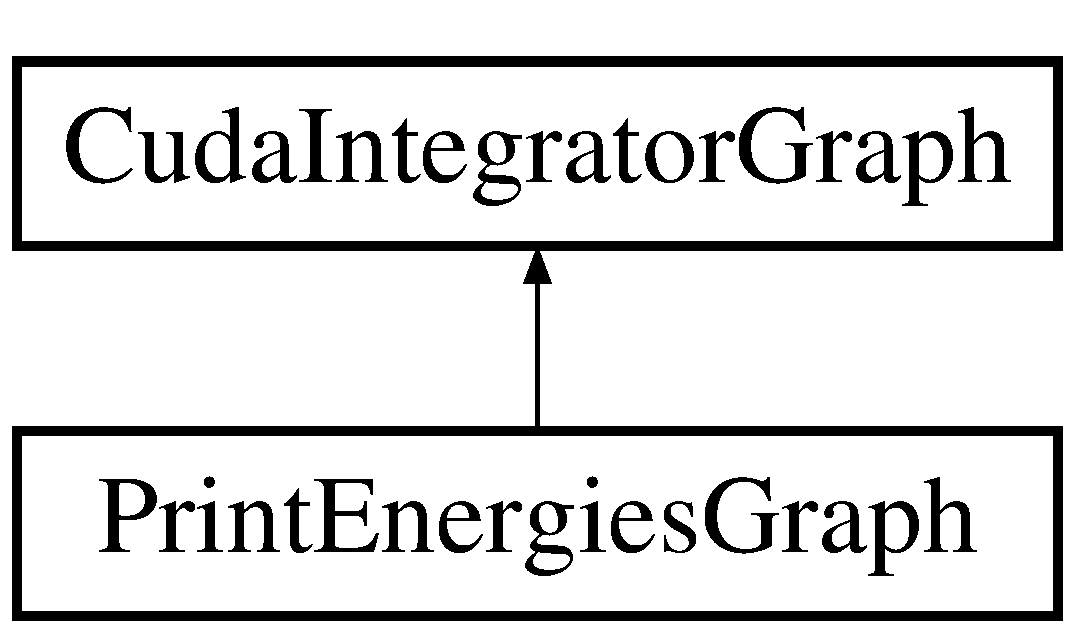
\includegraphics[height=2.000000cm]{classPrintEnergiesGraph}
\end{center}
\end{figure}
\subsection*{Public Member Functions}
\begin{DoxyCompactItemize}
\item 
\hypertarget{classPrintEnergiesGraph_a0dc6851ffca92ab37548e4be1a3578ff}{}\label{classPrintEnergiesGraph_a0dc6851ffca92ab37548e4be1a3578ff} 
{\bfseries Print\+Energies\+Graph} (\hyperlink{structPrintEnergiesGraphInputs}{Print\+Energies\+Graph\+Inputs} in)
\end{DoxyCompactItemize}
\subsection*{Additional Inherited Members}


\subsection{Detailed Description}
Create a graph to print the system energies. 

Example\+: Potential Energy,0,Kinetic Energy,0,Box Piston Potential Energy,0,Box Piston Kinetic Energy,0 

The documentation for this class was generated from the following file\+:\begin{DoxyCompactItemize}
\item 
/u/samar/\+Documents/git/chcuda/include/\hyperlink{PrintEnergiesGraph_8h}{Print\+Energies\+Graph.\+h}\end{DoxyCompactItemize}

\hypertarget{structPrintEnergiesGraphInputs}{}\section{Print\+Energies\+Graph\+Inputs Struct Reference}
\label{structPrintEnergiesGraphInputs}\index{Print\+Energies\+Graph\+Inputs@{Print\+Energies\+Graph\+Inputs}}


input for the graph that prints out the components of the total system energy.  




{\ttfamily \#include $<$Print\+Energies\+Graph.\+h$>$}

\subsection*{Public Attributes}
\begin{DoxyCompactItemize}
\item 
const double4 $\ast$\+\_\+\+\_\+restrict\+\_\+\+\_\+ \hyperlink{structPrintEnergiesGraphInputs_adc38d3e47b0b4ab22dfb7b0253ccefff}{velmass}
\begin{DoxyCompactList}\small\item\em Device pointer to Velocity and mass of each atom. \end{DoxyCompactList}\item 
const double $\ast$\+\_\+\+\_\+restrict\+\_\+\+\_\+ \hyperlink{structPrintEnergiesGraphInputs_a6faa1be5d040282aca80b029942ab2eb}{potential\+\_\+energy}
\begin{DoxyCompactList}\small\item\em Device pointer to potential of all atoms. \end{DoxyCompactList}\item 
const double3 $\ast$\+\_\+\+\_\+restrict\+\_\+\+\_\+ \hyperlink{structPrintEnergiesGraphInputs_a1e348a5a2a281ba456f7fa8955b43c02}{box}
\begin{DoxyCompactList}\small\item\em Device pointer to box dimensions. \end{DoxyCompactList}\item 
const double3 $\ast$\+\_\+\+\_\+restrict\+\_\+\+\_\+ \hyperlink{structPrintEnergiesGraphInputs_a19e4bdc53ef87010bb737cb6860ec653}{box\+\_\+dot}
\begin{DoxyCompactList}\small\item\em Device pointer to time derivative of box dimensions. \end{DoxyCompactList}\item 
\hyperlink{structVolumePiston}{Volume\+Piston} \hyperlink{structPrintEnergiesGraphInputs_a37b64e2334e0ee6481ecb96081417f2a}{piston}
\begin{DoxyCompactList}\small\item\em Piston Parameters. \end{DoxyCompactList}\item 
int \hyperlink{structPrintEnergiesGraphInputs_a959260c65f04a41a113f62ef76504966}{num\+Atoms}
\begin{DoxyCompactList}\small\item\em Number of Atoms. \end{DoxyCompactList}\end{DoxyCompactItemize}


\subsection{Detailed Description}
input for the graph that prints out the components of the total system energy. 



\subsection{Member Data Documentation}
\hypertarget{structPrintEnergiesGraphInputs_a1e348a5a2a281ba456f7fa8955b43c02}{}\label{structPrintEnergiesGraphInputs_a1e348a5a2a281ba456f7fa8955b43c02} 
\index{Print\+Energies\+Graph\+Inputs@{Print\+Energies\+Graph\+Inputs}!box@{box}}
\index{box@{box}!Print\+Energies\+Graph\+Inputs@{Print\+Energies\+Graph\+Inputs}}
\subsubsection{\texorpdfstring{box}{box}}
{\footnotesize\ttfamily const double3$\ast$ \+\_\+\+\_\+restrict\+\_\+\+\_\+ Print\+Energies\+Graph\+Inputs\+::box}



Device pointer to box dimensions. 

\hypertarget{structPrintEnergiesGraphInputs_a19e4bdc53ef87010bb737cb6860ec653}{}\label{structPrintEnergiesGraphInputs_a19e4bdc53ef87010bb737cb6860ec653} 
\index{Print\+Energies\+Graph\+Inputs@{Print\+Energies\+Graph\+Inputs}!box\+\_\+dot@{box\+\_\+dot}}
\index{box\+\_\+dot@{box\+\_\+dot}!Print\+Energies\+Graph\+Inputs@{Print\+Energies\+Graph\+Inputs}}
\subsubsection{\texorpdfstring{box\+\_\+dot}{box\_dot}}
{\footnotesize\ttfamily const double3$\ast$ \+\_\+\+\_\+restrict\+\_\+\+\_\+ Print\+Energies\+Graph\+Inputs\+::box\+\_\+dot}



Device pointer to time derivative of box dimensions. 

\hypertarget{structPrintEnergiesGraphInputs_a959260c65f04a41a113f62ef76504966}{}\label{structPrintEnergiesGraphInputs_a959260c65f04a41a113f62ef76504966} 
\index{Print\+Energies\+Graph\+Inputs@{Print\+Energies\+Graph\+Inputs}!num\+Atoms@{num\+Atoms}}
\index{num\+Atoms@{num\+Atoms}!Print\+Energies\+Graph\+Inputs@{Print\+Energies\+Graph\+Inputs}}
\subsubsection{\texorpdfstring{num\+Atoms}{numAtoms}}
{\footnotesize\ttfamily int Print\+Energies\+Graph\+Inputs\+::num\+Atoms}



Number of Atoms. 

\hypertarget{structPrintEnergiesGraphInputs_a37b64e2334e0ee6481ecb96081417f2a}{}\label{structPrintEnergiesGraphInputs_a37b64e2334e0ee6481ecb96081417f2a} 
\index{Print\+Energies\+Graph\+Inputs@{Print\+Energies\+Graph\+Inputs}!piston@{piston}}
\index{piston@{piston}!Print\+Energies\+Graph\+Inputs@{Print\+Energies\+Graph\+Inputs}}
\subsubsection{\texorpdfstring{piston}{piston}}
{\footnotesize\ttfamily \hyperlink{structVolumePiston}{Volume\+Piston} Print\+Energies\+Graph\+Inputs\+::piston}



Piston Parameters. 

\hypertarget{structPrintEnergiesGraphInputs_a6faa1be5d040282aca80b029942ab2eb}{}\label{structPrintEnergiesGraphInputs_a6faa1be5d040282aca80b029942ab2eb} 
\index{Print\+Energies\+Graph\+Inputs@{Print\+Energies\+Graph\+Inputs}!potential\+\_\+energy@{potential\+\_\+energy}}
\index{potential\+\_\+energy@{potential\+\_\+energy}!Print\+Energies\+Graph\+Inputs@{Print\+Energies\+Graph\+Inputs}}
\subsubsection{\texorpdfstring{potential\+\_\+energy}{potential\_energy}}
{\footnotesize\ttfamily const double$\ast$ \+\_\+\+\_\+restrict\+\_\+\+\_\+ Print\+Energies\+Graph\+Inputs\+::potential\+\_\+energy}



Device pointer to potential of all atoms. 

\hypertarget{structPrintEnergiesGraphInputs_adc38d3e47b0b4ab22dfb7b0253ccefff}{}\label{structPrintEnergiesGraphInputs_adc38d3e47b0b4ab22dfb7b0253ccefff} 
\index{Print\+Energies\+Graph\+Inputs@{Print\+Energies\+Graph\+Inputs}!velmass@{velmass}}
\index{velmass@{velmass}!Print\+Energies\+Graph\+Inputs@{Print\+Energies\+Graph\+Inputs}}
\subsubsection{\texorpdfstring{velmass}{velmass}}
{\footnotesize\ttfamily const double4$\ast$ \+\_\+\+\_\+restrict\+\_\+\+\_\+ Print\+Energies\+Graph\+Inputs\+::velmass}



Device pointer to Velocity and mass of each atom. 



The documentation for this struct was generated from the following file\+:\begin{DoxyCompactItemize}
\item 
/u/samar/\+Documents/git/chcuda/include/\hyperlink{PrintEnergiesGraph_8h}{Print\+Energies\+Graph.\+h}\end{DoxyCompactItemize}

\hypertarget{structr123_1_1ReinterpretCtr}{}\section{r123\+:\+:Reinterpret\+Ctr$<$ To\+Type, C\+B\+R\+NG $>$ Struct Template Reference}
\label{structr123_1_1ReinterpretCtr}\index{r123\+::\+Reinterpret\+Ctr$<$ To\+Type, C\+B\+R\+N\+G $>$@{r123\+::\+Reinterpret\+Ctr$<$ To\+Type, C\+B\+R\+N\+G $>$}}


{\ttfamily \#include $<$Reinterpret\+Ctr.\+hpp$>$}

\subsection*{Public Types}
\begin{DoxyCompactItemize}
\item 
\hypertarget{structr123_1_1ReinterpretCtr_a26cf9e933b35411c37070c948085ba02}{}\label{structr123_1_1ReinterpretCtr_a26cf9e933b35411c37070c948085ba02} 
typedef To\+Type {\bfseries ctr\+\_\+type}
\item 
\hypertarget{structr123_1_1ReinterpretCtr_a470b21676ed709aa9d9ad524a67410f1}{}\label{structr123_1_1ReinterpretCtr_a470b21676ed709aa9d9ad524a67410f1} 
typedef C\+B\+R\+N\+G\+::key\+\_\+type {\bfseries key\+\_\+type}
\item 
\hypertarget{structr123_1_1ReinterpretCtr_ae0accaee618b5eb28a24acd516b3a4c6}{}\label{structr123_1_1ReinterpretCtr_ae0accaee618b5eb28a24acd516b3a4c6} 
typedef C\+B\+R\+N\+G\+::ctr\+\_\+type {\bfseries bctype}
\item 
\hypertarget{structr123_1_1ReinterpretCtr_a4b0b69c1aa58d62bb22e51e16c586bee}{}\label{structr123_1_1ReinterpretCtr_a4b0b69c1aa58d62bb22e51e16c586bee} 
typedef C\+B\+R\+N\+G\+::ukey\+\_\+type {\bfseries ukey\+\_\+type}
\end{DoxyCompactItemize}
\subsection*{Public Member Functions}
\begin{DoxyCompactItemize}
\item 
\hypertarget{structr123_1_1ReinterpretCtr_ad6fe140cb2f1aa215c4741f646249b16}{}\label{structr123_1_1ReinterpretCtr_ad6fe140cb2f1aa215c4741f646249b16} 
{\bfseries R123\+\_\+\+S\+T\+A\+T\+I\+C\+\_\+\+A\+S\+S\+E\+RT} (sizeof(To\+Type)==sizeof(bctype) \&\&sizeof(typename bctype\+::value\+\_\+type) !=16, \char`\"{}Reinterpret\+Ctr\+:  sizeof(To\+Type) is not the same as sizeof(C\+B\+R\+N\+G\+::ctr\+\_\+type) or C\+B\+R\+N\+G\+::ctr\+\_\+type\+::value\+\_\+type looks like it might be \+\_\+\+\_\+m128i\char`\"{})
\item 
\hypertarget{structr123_1_1ReinterpretCtr_a91edc5103397372cc5509ad17c0fc83a}{}\label{structr123_1_1ReinterpretCtr_a91edc5103397372cc5509ad17c0fc83a} 
ctr\+\_\+type {\bfseries operator()} (ctr\+\_\+type c, key\+\_\+type k)
\end{DoxyCompactItemize}


\subsection{Detailed Description}
\subsubsection*{template$<$typename To\+Type, typename C\+B\+R\+NG$>$\newline
struct r123\+::\+Reinterpret\+Ctr$<$ To\+Type, C\+B\+R\+N\+G $>$}

\hyperlink{structr123_1_1ReinterpretCtr}{Reinterpret\+Ctr} uses memcpy to map back and forth between a C\+B\+R\+NG\textquotesingle{}s ctr\+\_\+type and the specified To\+Type. For example, after\+:

typedef Reinterpret\+Ctr$<$r123array4x32, Philox2x64$>$ G;

G is a bona fide C\+B\+R\+NG with ctr\+\_\+type r123array4x32.

W\+A\+R\+N\+I\+NG\+: \hyperlink{structr123_1_1ReinterpretCtr}{Reinterpret\+Ctr} is endian dependent. The values returned by G, declared as above, will depend on the endianness of the machine on which it runs. 

The documentation for this struct was generated from the following file\+:\begin{DoxyCompactItemize}
\item 
/u/samar/\+Documents/git/chcuda/include/\+Random123/Reinterpret\+Ctr.\+hpp\end{DoxyCompactItemize}

\hypertarget{classSimpleLeapfrogGraph}{}\section{Simple\+Leapfrog\+Graph Class Reference}
\label{classSimpleLeapfrogGraph}\index{Simple\+Leapfrog\+Graph@{Simple\+Leapfrog\+Graph}}


Create a graph to do the simple leapfrog integration.  




{\ttfamily \#include $<$Simple\+Leapfrog\+Graph.\+h$>$}

Inheritance diagram for Simple\+Leapfrog\+Graph\+:\begin{figure}[H]
\begin{center}
\leavevmode
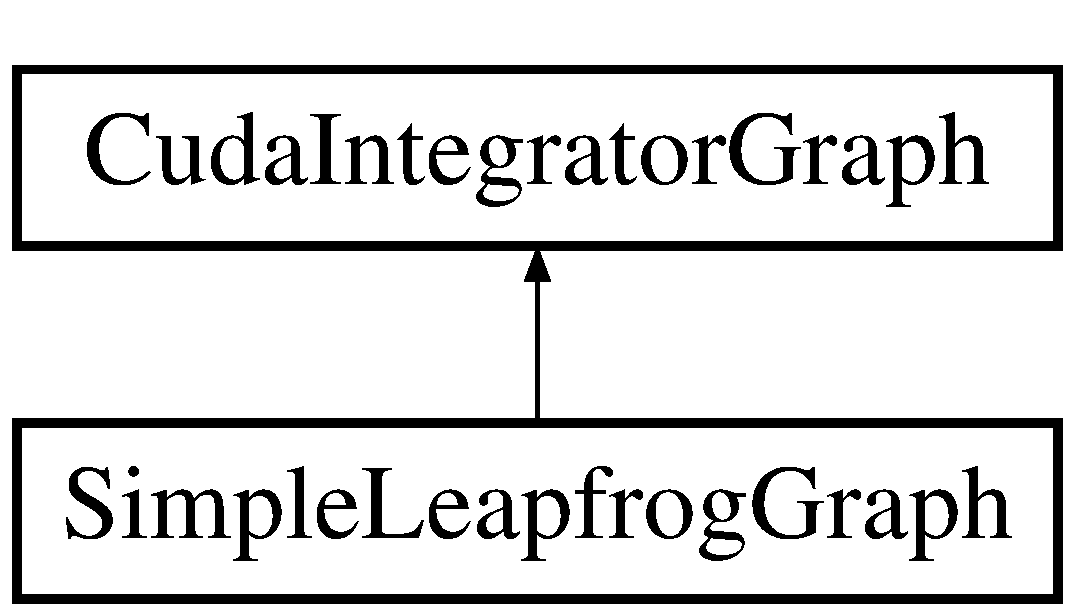
\includegraphics[height=2.000000cm]{classSimpleLeapfrogGraph}
\end{center}
\end{figure}
\subsection*{Public Member Functions}
\begin{DoxyCompactItemize}
\item 
\hypertarget{classSimpleLeapfrogGraph_a7cb32aee82e9d3d809b792e3f59cdcf1}{}\label{classSimpleLeapfrogGraph_a7cb32aee82e9d3d809b792e3f59cdcf1} 
{\bfseries Simple\+Leapfrog\+Graph} (\hyperlink{structSimpleLeapfrogGraphInputs}{Simple\+Leapfrog\+Graph\+Inputs} in)
\end{DoxyCompactItemize}
\subsection*{Additional Inherited Members}


\subsection{Detailed Description}
Create a graph to do the simple leapfrog integration. 



The documentation for this class was generated from the following file\+:\begin{DoxyCompactItemize}
\item 
/u/samar/\+Documents/git/chcuda/include/\hyperlink{SimpleLeapfrogGraph_8h}{Simple\+Leapfrog\+Graph.\+h}\end{DoxyCompactItemize}

\hypertarget{structSimpleLeapfrogGraphInputs}{}\section{Simple\+Leapfrog\+Graph\+Inputs Struct Reference}
\label{structSimpleLeapfrogGraphInputs}\index{Simple\+Leapfrog\+Graph\+Inputs@{Simple\+Leapfrog\+Graph\+Inputs}}


Struct for Simple leapfrog kernel input.  




{\ttfamily \#include $<$Simple\+Leapfrog\+Graph.\+h$>$}

\subsection*{Public Attributes}
\begin{DoxyCompactItemize}
\item 
const double4 $\ast$ \hyperlink{structSimpleLeapfrogGraphInputs_a01fc1ca37ad0127b87feb3d757d6f41c}{old\+\_\+xyzq}
\begin{DoxyCompactList}\small\item\em Device pointer to old positions. \end{DoxyCompactList}\item 
const double4 $\ast$ \hyperlink{structSimpleLeapfrogGraphInputs_a0bc70243226e08c936bb36c5dcaa37cc}{old\+\_\+velmass}
\begin{DoxyCompactList}\small\item\em Device pointer to old velocity. \end{DoxyCompactList}\item 
const double4 $\ast$\+\_\+\+\_\+restrict\+\_\+\+\_\+ \hyperlink{structSimpleLeapfrogGraphInputs_a0f2c8a7955eede32a5ae9be6fcf9c894}{force\+\_\+invmass}
\begin{DoxyCompactList}\small\item\em Device pointer to force inverse mass. \end{DoxyCompactList}\item 
double4 $\ast$ \hyperlink{structSimpleLeapfrogGraphInputs_a769f1661c0f9d43ffa98066b106049ab}{new\+\_\+xyzq}
\begin{DoxyCompactList}\small\item\em Device pointer to new positions. \end{DoxyCompactList}\item 
double4 $\ast$ \hyperlink{structSimpleLeapfrogGraphInputs_aaacb07a926ff1a46ac5c8d0edc21d2af}{new\+\_\+velmass}
\begin{DoxyCompactList}\small\item\em Device pointer to new velocities. \end{DoxyCompactList}\item 
int \hyperlink{structSimpleLeapfrogGraphInputs_af774c2d3b4033330bb43cbbe3398059f}{num\+Atoms}
\begin{DoxyCompactList}\small\item\em Number of atoms. \end{DoxyCompactList}\item 
double \hyperlink{structSimpleLeapfrogGraphInputs_a197aa8d9f5695cda2406de1aff9b4e3b}{timestep}
\begin{DoxyCompactList}\small\item\em Time step. \end{DoxyCompactList}\end{DoxyCompactItemize}


\subsection{Detailed Description}
Struct for Simple leapfrog kernel input. 

\subsection{Member Data Documentation}
\hypertarget{structSimpleLeapfrogGraphInputs_a0f2c8a7955eede32a5ae9be6fcf9c894}{}\label{structSimpleLeapfrogGraphInputs_a0f2c8a7955eede32a5ae9be6fcf9c894} 
\index{Simple\+Leapfrog\+Graph\+Inputs@{Simple\+Leapfrog\+Graph\+Inputs}!force\+\_\+invmass@{force\+\_\+invmass}}
\index{force\+\_\+invmass@{force\+\_\+invmass}!Simple\+Leapfrog\+Graph\+Inputs@{Simple\+Leapfrog\+Graph\+Inputs}}
\subsubsection{\texorpdfstring{force\+\_\+invmass}{force\_invmass}}
{\footnotesize\ttfamily const double4$\ast$ \+\_\+\+\_\+restrict\+\_\+\+\_\+ Simple\+Leapfrog\+Graph\+Inputs\+::force\+\_\+invmass}



Device pointer to force inverse mass. 

\hypertarget{structSimpleLeapfrogGraphInputs_aaacb07a926ff1a46ac5c8d0edc21d2af}{}\label{structSimpleLeapfrogGraphInputs_aaacb07a926ff1a46ac5c8d0edc21d2af} 
\index{Simple\+Leapfrog\+Graph\+Inputs@{Simple\+Leapfrog\+Graph\+Inputs}!new\+\_\+velmass@{new\+\_\+velmass}}
\index{new\+\_\+velmass@{new\+\_\+velmass}!Simple\+Leapfrog\+Graph\+Inputs@{Simple\+Leapfrog\+Graph\+Inputs}}
\subsubsection{\texorpdfstring{new\+\_\+velmass}{new\_velmass}}
{\footnotesize\ttfamily double4$\ast$ Simple\+Leapfrog\+Graph\+Inputs\+::new\+\_\+velmass}



Device pointer to new velocities. 

\hypertarget{structSimpleLeapfrogGraphInputs_a769f1661c0f9d43ffa98066b106049ab}{}\label{structSimpleLeapfrogGraphInputs_a769f1661c0f9d43ffa98066b106049ab} 
\index{Simple\+Leapfrog\+Graph\+Inputs@{Simple\+Leapfrog\+Graph\+Inputs}!new\+\_\+xyzq@{new\+\_\+xyzq}}
\index{new\+\_\+xyzq@{new\+\_\+xyzq}!Simple\+Leapfrog\+Graph\+Inputs@{Simple\+Leapfrog\+Graph\+Inputs}}
\subsubsection{\texorpdfstring{new\+\_\+xyzq}{new\_xyzq}}
{\footnotesize\ttfamily double4$\ast$ Simple\+Leapfrog\+Graph\+Inputs\+::new\+\_\+xyzq}



Device pointer to new positions. 

\hypertarget{structSimpleLeapfrogGraphInputs_af774c2d3b4033330bb43cbbe3398059f}{}\label{structSimpleLeapfrogGraphInputs_af774c2d3b4033330bb43cbbe3398059f} 
\index{Simple\+Leapfrog\+Graph\+Inputs@{Simple\+Leapfrog\+Graph\+Inputs}!num\+Atoms@{num\+Atoms}}
\index{num\+Atoms@{num\+Atoms}!Simple\+Leapfrog\+Graph\+Inputs@{Simple\+Leapfrog\+Graph\+Inputs}}
\subsubsection{\texorpdfstring{num\+Atoms}{numAtoms}}
{\footnotesize\ttfamily int Simple\+Leapfrog\+Graph\+Inputs\+::num\+Atoms}



Number of atoms. 

\hypertarget{structSimpleLeapfrogGraphInputs_a0bc70243226e08c936bb36c5dcaa37cc}{}\label{structSimpleLeapfrogGraphInputs_a0bc70243226e08c936bb36c5dcaa37cc} 
\index{Simple\+Leapfrog\+Graph\+Inputs@{Simple\+Leapfrog\+Graph\+Inputs}!old\+\_\+velmass@{old\+\_\+velmass}}
\index{old\+\_\+velmass@{old\+\_\+velmass}!Simple\+Leapfrog\+Graph\+Inputs@{Simple\+Leapfrog\+Graph\+Inputs}}
\subsubsection{\texorpdfstring{old\+\_\+velmass}{old\_velmass}}
{\footnotesize\ttfamily const double4$\ast$ Simple\+Leapfrog\+Graph\+Inputs\+::old\+\_\+velmass}



Device pointer to old velocity. 

\hypertarget{structSimpleLeapfrogGraphInputs_a01fc1ca37ad0127b87feb3d757d6f41c}{}\label{structSimpleLeapfrogGraphInputs_a01fc1ca37ad0127b87feb3d757d6f41c} 
\index{Simple\+Leapfrog\+Graph\+Inputs@{Simple\+Leapfrog\+Graph\+Inputs}!old\+\_\+xyzq@{old\+\_\+xyzq}}
\index{old\+\_\+xyzq@{old\+\_\+xyzq}!Simple\+Leapfrog\+Graph\+Inputs@{Simple\+Leapfrog\+Graph\+Inputs}}
\subsubsection{\texorpdfstring{old\+\_\+xyzq}{old\_xyzq}}
{\footnotesize\ttfamily const double4$\ast$ Simple\+Leapfrog\+Graph\+Inputs\+::old\+\_\+xyzq}



Device pointer to old positions. 

\hypertarget{structSimpleLeapfrogGraphInputs_a197aa8d9f5695cda2406de1aff9b4e3b}{}\label{structSimpleLeapfrogGraphInputs_a197aa8d9f5695cda2406de1aff9b4e3b} 
\index{Simple\+Leapfrog\+Graph\+Inputs@{Simple\+Leapfrog\+Graph\+Inputs}!timestep@{timestep}}
\index{timestep@{timestep}!Simple\+Leapfrog\+Graph\+Inputs@{Simple\+Leapfrog\+Graph\+Inputs}}
\subsubsection{\texorpdfstring{timestep}{timestep}}
{\footnotesize\ttfamily double Simple\+Leapfrog\+Graph\+Inputs\+::timestep}



Time step. 



The documentation for this struct was generated from the following file\+:\begin{DoxyCompactItemize}
\item 
/u/samar/\+Documents/git/chcuda/include/\hyperlink{SimpleLeapfrogGraph_8h}{Simple\+Leapfrog\+Graph.\+h}\end{DoxyCompactItemize}

\hypertarget{structsolvent__t}{}\section{solvent\+\_\+t Struct Reference}
\label{structsolvent__t}\index{solvent\+\_\+t@{solvent\+\_\+t}}
\subsection*{Public Member Functions}
\begin{DoxyCompactItemize}
\item 
\hypertarget{structsolvent__t_abb12339e961b188e294d6a209519914a}{}\label{structsolvent__t_abb12339e961b188e294d6a209519914a} 
void {\bfseries get\+Atoms} (std\+::vector$<$ int $>$ \&atoms)
\item 
\hypertarget{structsolvent__t_acb88ad579fe69328d85c98c1580e4ac9}{}\label{structsolvent__t_acb88ad579fe69328d85c98c1580e4ac9} 
void {\bfseries print\+Atoms} ()
\end{DoxyCompactItemize}
\subsection*{Static Public Member Functions}
\begin{DoxyCompactItemize}
\item 
\hypertarget{structsolvent__t_ab9c4a3d933fc7bf8e3698537017e1a65}{}\label{structsolvent__t_ab9c4a3d933fc7bf8e3698537017e1a65} 
static int {\bfseries type} ()
\item 
\hypertarget{structsolvent__t_ad7c3bb92e9feb6fb74bea84300bb6027}{}\label{structsolvent__t_ad7c3bb92e9feb6fb74bea84300bb6027} 
static int {\bfseries size} ()
\end{DoxyCompactItemize}
\subsection*{Public Attributes}
\begin{DoxyCompactItemize}
\item 
\hypertarget{structsolvent__t_a39316277b1789a8c31526b171f2cd451}{}\label{structsolvent__t_a39316277b1789a8c31526b171f2cd451} 
int {\bfseries i}
\item 
\hypertarget{structsolvent__t_aedb4a6a1e76573817c726b80d8c4c006}{}\label{structsolvent__t_aedb4a6a1e76573817c726b80d8c4c006} 
int {\bfseries j}
\item 
\hypertarget{structsolvent__t_a2aee343736906059dd2959a335084ed3}{}\label{structsolvent__t_a2aee343736906059dd2959a335084ed3} 
int {\bfseries k}
\end{DoxyCompactItemize}


The documentation for this struct was generated from the following file\+:\begin{DoxyCompactItemize}
\item 
/u/samar/\+Documents/git/chcuda/include/Bonded\+\_\+struct.\+h\end{DoxyCompactItemize}

\hypertarget{structtile__excl__t}{}\section{tile\+\_\+excl\+\_\+t$<$ tilesize $>$ Struct Template Reference}
\label{structtile__excl__t}\index{tile\+\_\+excl\+\_\+t$<$ tilesize $>$@{tile\+\_\+excl\+\_\+t$<$ tilesize $>$}}
\subsection*{Public Attributes}
\begin{DoxyCompactItemize}
\item 
\hypertarget{structtile__excl__t_a3150bae21a288b5f1aaba959b3486d4f}{}\label{structtile__excl__t_a3150bae21a288b5f1aaba959b3486d4f} 
unsigned int {\bfseries excl} \mbox{[}\hyperlink{structnum__excl}{num\+\_\+excl}$<$ tilesize $>$\+::val\mbox{]}
\end{DoxyCompactItemize}


The documentation for this struct was generated from the following file\+:\begin{DoxyCompactItemize}
\item 
/u/samar/\+Documents/git/chcuda/include/Cuda\+Neighbor\+List\+Build.\+h\end{DoxyCompactItemize}

\hypertarget{structVirial__t}{}\section{Virial\+\_\+t Struct Reference}
\label{structVirial__t}\index{Virial\+\_\+t@{Virial\+\_\+t}}
\subsection*{Public Attributes}
\begin{DoxyCompactItemize}
\item 
\hypertarget{structVirial__t_a05e5da9bdb44f9521b59ad77bfe13b35}{}\label{structVirial__t_a05e5da9bdb44f9521b59ad77bfe13b35} 
double {\bfseries sforce\+\_\+dp} \mbox{[}27\mbox{]}\mbox{[}3\mbox{]}
\item 
\hypertarget{structVirial__t_a03d714e3786a305fd1d695cff594b802}{}\label{structVirial__t_a03d714e3786a305fd1d695cff594b802} 
long long int {\bfseries sforce\+\_\+fp} \mbox{[}27\mbox{]}\mbox{[}3\mbox{]}
\item 
\hypertarget{structVirial__t_a9a17b06589f2174d1892904f470dc95e}{}\label{structVirial__t_a9a17b06589f2174d1892904f470dc95e} 
double {\bfseries virmat} \mbox{[}9\mbox{]}
\end{DoxyCompactItemize}


The documentation for this struct was generated from the following file\+:\begin{DoxyCompactItemize}
\item 
/u/samar/\+Documents/git/chcuda/include/Cuda\+Energy\+Virial.\+h\end{DoxyCompactItemize}

\hypertarget{structVolumePiston}{}\section{Volume\+Piston Struct Reference}
\label{structVolumePiston}\index{Volume\+Piston@{Volume\+Piston}}


Struct to hold the volume piston parameters and some functions to help with dynamics.  




{\ttfamily \#include $<$Volume\+Piston.\+h$>$}

\subsection*{Public Member Functions}
\begin{DoxyCompactItemize}
\item 
\hypertarget{structVolumePiston_a739d6b6559f8e7861ed9f606e87cc2d9}{}\label{structVolumePiston_a739d6b6559f8e7861ed9f606e87cc2d9} 
C\+U\+D\+A\+\_\+\+C\+A\+L\+L\+A\+B\+L\+E\+\_\+\+M\+E\+M\+B\+ER double {\bfseries calcpe} (double3 box) const
\item 
\hypertarget{structVolumePiston_ac699322cd986cf421e79efc1bbedc45c}{}\label{structVolumePiston_ac699322cd986cf421e79efc1bbedc45c} 
C\+U\+D\+A\+\_\+\+C\+A\+L\+L\+A\+B\+L\+E\+\_\+\+M\+E\+M\+B\+ER double {\bfseries calcke} (double3 box, double3 box\+\_\+dot) const
\item 
C\+U\+D\+A\+\_\+\+C\+A\+L\+L\+A\+B\+L\+E\+\_\+\+M\+E\+M\+B\+ER void \hyperlink{structVolumePiston_a771864206ceef0f0ae6c07e1639a8d71}{leapfrogdrift} (const double3 $\ast$old\+\_\+com\+\_\+ke, const double3 $\ast$old\+\_\+box, const double3 $\ast$old\+\_\+box\+\_\+dot, double3 $\ast$new\+\_\+com\+\_\+ke, double3 $\ast$new\+\_\+box, double3 $\ast$new\+\_\+box\+\_\+dot, double3 $\ast$\+\_\+\+\_\+restrict\+\_\+\+\_\+ com\+\_\+momentum\+\_\+scale, double3 $\ast$\+\_\+\+\_\+restrict\+\_\+\+\_\+ com\+\_\+momentum\+\_\+prescale, double3 $\ast$\+\_\+\+\_\+restrict\+\_\+\+\_\+ com\+\_\+position\+\_\+prescale, double timestep) const
\item 
C\+U\+D\+A\+\_\+\+C\+A\+L\+L\+A\+B\+L\+E\+\_\+\+M\+E\+M\+B\+ER void \hyperlink{structVolumePiston_ae2ae90b94c4f05a5338a2599a5e12f96}{pressure\+Kick} (const double3 $\ast$\+\_\+\+\_\+restrict\+\_\+\+\_\+ box, const double3 $\ast$old\+\_\+box\+\_\+dot, double3 $\ast$new\+\_\+box\+\_\+dot, double timestep) const
\item 
C\+U\+D\+A\+\_\+\+C\+A\+L\+L\+A\+B\+L\+E\+\_\+\+M\+E\+M\+B\+ER void \hyperlink{structVolumePiston_ab1d3d87cae459ab285f52c694cfa35f0}{virial\+Kick} (const double3 $\ast$\+\_\+\+\_\+restrict\+\_\+\+\_\+ virial, const double3 $\ast$\+\_\+\+\_\+restrict\+\_\+\+\_\+ box, const double3 $\ast$old\+\_\+box\+\_\+dot, double3 $\ast$new\+\_\+box\+\_\+dot, double timestep) const
\item 
C\+U\+D\+A\+\_\+\+C\+A\+L\+L\+A\+B\+L\+E\+\_\+\+M\+E\+M\+B\+ER void \hyperlink{structVolumePiston_af199572d24c18206fa173f6f24c637f5}{kinetic\+Energy\+Kick} (const double3 $\ast$\+\_\+\+\_\+restrict\+\_\+\+\_\+ com\+\_\+ke, const double3 $\ast$\+\_\+\+\_\+restrict\+\_\+\+\_\+ box, const double3 $\ast$old\+\_\+box\+\_\+dot, double3 $\ast$new\+\_\+box\+\_\+dot, double timestep) const
\end{DoxyCompactItemize}
\subsection*{Public Attributes}
\begin{DoxyCompactItemize}
\item 
double \hyperlink{structVolumePiston_aff364bf76db0d8e73d251dccf2301193}{pressure}
\begin{DoxyCompactList}\small\item\em Reference pressure, units are not atms, it is SI compatible with other units. \end{DoxyCompactList}\item 
double \hyperlink{structVolumePiston_a831ba454760bec711a2823f432b21840}{piston\+\_\+mass}
\begin{DoxyCompactList}\small\item\em Piston Mass, dimensions of mass/length$^\wedge$4. \end{DoxyCompactList}\end{DoxyCompactItemize}


\subsection{Detailed Description}
Struct to hold the volume piston parameters and some functions to help with dynamics. 



\subsection{Member Function Documentation}
\hypertarget{structVolumePiston_af199572d24c18206fa173f6f24c637f5}{}\label{structVolumePiston_af199572d24c18206fa173f6f24c637f5} 
\index{Volume\+Piston@{Volume\+Piston}!kinetic\+Energy\+Kick@{kinetic\+Energy\+Kick}}
\index{kinetic\+Energy\+Kick@{kinetic\+Energy\+Kick}!Volume\+Piston@{Volume\+Piston}}
\subsubsection{\texorpdfstring{kinetic\+Energy\+Kick()}{kineticEnergyKick()}}
{\footnotesize\ttfamily C\+U\+D\+A\+\_\+\+C\+A\+L\+L\+A\+B\+L\+E\+\_\+\+M\+E\+M\+B\+ER void Volume\+Piston\+::kinetic\+Energy\+Kick (\begin{DoxyParamCaption}\item[{const double3 $\ast$\+\_\+\+\_\+restrict\+\_\+\+\_\+}]{com\+\_\+ke,  }\item[{const double3 $\ast$\+\_\+\+\_\+restrict\+\_\+\+\_\+}]{box,  }\item[{const double3 $\ast$}]{old\+\_\+box\+\_\+dot,  }\item[{double3 $\ast$}]{new\+\_\+box\+\_\+dot,  }\item[{double}]{timestep }\end{DoxyParamCaption}) const\hspace{0.3cm}{\ttfamily [inline]}}


\begin{DoxyParams}{Parameters}
{\em com\+\_\+ke} & Pointer to kinetic energy of pressure group momentums \\
\hline
{\em box} & Pointer to box lengths \\
\hline
{\em old\+\_\+box\+\_\+dot} & Pointer to box length time dirivatives \\
\hline
{\em new\+\_\+box\+\_\+dot} & Pointer to save post drift box length time dirivatives \\
\hline
{\em timestep} & Time step. \\
\hline
\end{DoxyParams}
\hypertarget{structVolumePiston_a771864206ceef0f0ae6c07e1639a8d71}{}\label{structVolumePiston_a771864206ceef0f0ae6c07e1639a8d71} 
\index{Volume\+Piston@{Volume\+Piston}!leapfrogdrift@{leapfrogdrift}}
\index{leapfrogdrift@{leapfrogdrift}!Volume\+Piston@{Volume\+Piston}}
\subsubsection{\texorpdfstring{leapfrogdrift()}{leapfrogdrift()}}
{\footnotesize\ttfamily C\+U\+D\+A\+\_\+\+C\+A\+L\+L\+A\+B\+L\+E\+\_\+\+M\+E\+M\+B\+ER void Volume\+Piston\+::leapfrogdrift (\begin{DoxyParamCaption}\item[{const double3 $\ast$}]{old\+\_\+com\+\_\+ke,  }\item[{const double3 $\ast$}]{old\+\_\+box,  }\item[{const double3 $\ast$}]{old\+\_\+box\+\_\+dot,  }\item[{double3 $\ast$}]{new\+\_\+com\+\_\+ke,  }\item[{double3 $\ast$}]{new\+\_\+box,  }\item[{double3 $\ast$}]{new\+\_\+box\+\_\+dot,  }\item[{double3 $\ast$\+\_\+\+\_\+restrict\+\_\+\+\_\+}]{com\+\_\+momentum\+\_\+scale,  }\item[{double3 $\ast$\+\_\+\+\_\+restrict\+\_\+\+\_\+}]{com\+\_\+momentum\+\_\+prescale,  }\item[{double3 $\ast$\+\_\+\+\_\+restrict\+\_\+\+\_\+}]{com\+\_\+position\+\_\+prescale,  }\item[{double}]{timestep }\end{DoxyParamCaption}) const\hspace{0.3cm}{\ttfamily [inline]}}


\begin{DoxyParams}{Parameters}
{\em old\+\_\+com\+\_\+ke} & Pointer to kinetic energy of pressure group momentums \\
\hline
{\em old\+\_\+box} & Pointer to box lengths \\
\hline
{\em old\+\_\+box\+\_\+dot} & Pointer to box length time dirivatives \\
\hline
{\em new\+\_\+com\+\_\+ke} & Pointer to save post drift pressure group momentum kinetic energy \\
\hline
{\em new\+\_\+box} & Pointer to save post drift box lengths \\
\hline
{\em new\+\_\+box\+\_\+dot} & Pointer to save post drift box length time dirivatives \\
\hline
{\em com\+\_\+momentum\+\_\+scale} & Pointer to final pressure group momentum scale. This is the total scale from predrift p group momentum to post drift p group momentum. \\
\hline
{\em com\+\_\+momentum\+\_\+prescale} & Pointer to initial pressure group momentum scale. This is the scaleing of momentum that happens before the pressure group centers of mass are moved. \\
\hline
{\em com\+\_\+position\+\_\+prescale} & Pointer to initial pressure group C\+OM scale. This is the scaling p group centers of mass before the are moved by their prescaled momenentums. \\
\hline
{\em timestep} & Time step. \\
\hline
\end{DoxyParams}
\hypertarget{structVolumePiston_ae2ae90b94c4f05a5338a2599a5e12f96}{}\label{structVolumePiston_ae2ae90b94c4f05a5338a2599a5e12f96} 
\index{Volume\+Piston@{Volume\+Piston}!pressure\+Kick@{pressure\+Kick}}
\index{pressure\+Kick@{pressure\+Kick}!Volume\+Piston@{Volume\+Piston}}
\subsubsection{\texorpdfstring{pressure\+Kick()}{pressureKick()}}
{\footnotesize\ttfamily C\+U\+D\+A\+\_\+\+C\+A\+L\+L\+A\+B\+L\+E\+\_\+\+M\+E\+M\+B\+ER void Volume\+Piston\+::pressure\+Kick (\begin{DoxyParamCaption}\item[{const double3 $\ast$\+\_\+\+\_\+restrict\+\_\+\+\_\+}]{box,  }\item[{const double3 $\ast$}]{old\+\_\+box\+\_\+dot,  }\item[{double3 $\ast$}]{new\+\_\+box\+\_\+dot,  }\item[{double}]{timestep }\end{DoxyParamCaption}) const\hspace{0.3cm}{\ttfamily [inline]}}


\begin{DoxyParams}{Parameters}
{\em box} & Pointer to box lengths \\
\hline
{\em old\+\_\+box\+\_\+dot} & Pointer to box length time dirivatives \\
\hline
{\em new\+\_\+box\+\_\+dot} & Pointer to save post drift box length time dirivatives \\
\hline
{\em timestep} & Time step. \\
\hline
\end{DoxyParams}
\hypertarget{structVolumePiston_ab1d3d87cae459ab285f52c694cfa35f0}{}\label{structVolumePiston_ab1d3d87cae459ab285f52c694cfa35f0} 
\index{Volume\+Piston@{Volume\+Piston}!virial\+Kick@{virial\+Kick}}
\index{virial\+Kick@{virial\+Kick}!Volume\+Piston@{Volume\+Piston}}
\subsubsection{\texorpdfstring{virial\+Kick()}{virialKick()}}
{\footnotesize\ttfamily C\+U\+D\+A\+\_\+\+C\+A\+L\+L\+A\+B\+L\+E\+\_\+\+M\+E\+M\+B\+ER void Volume\+Piston\+::virial\+Kick (\begin{DoxyParamCaption}\item[{const double3 $\ast$\+\_\+\+\_\+restrict\+\_\+\+\_\+}]{virial,  }\item[{const double3 $\ast$\+\_\+\+\_\+restrict\+\_\+\+\_\+}]{box,  }\item[{const double3 $\ast$}]{old\+\_\+box\+\_\+dot,  }\item[{double3 $\ast$}]{new\+\_\+box\+\_\+dot,  }\item[{double}]{timestep }\end{DoxyParamCaption}) const\hspace{0.3cm}{\ttfamily [inline]}}


\begin{DoxyParams}{Parameters}
{\em virial} & Pointer to corrected virial \\
\hline
{\em box} & Pointer to box lengths \\
\hline
{\em old\+\_\+box\+\_\+dot} & Pointer to box length time dirivatives \\
\hline
{\em new\+\_\+box\+\_\+dot} & Pointer to save post drift box length time dirivatives \\
\hline
{\em timestep} & Time step. \\
\hline
\end{DoxyParams}


\subsection{Member Data Documentation}
\hypertarget{structVolumePiston_a831ba454760bec711a2823f432b21840}{}\label{structVolumePiston_a831ba454760bec711a2823f432b21840} 
\index{Volume\+Piston@{Volume\+Piston}!piston\+\_\+mass@{piston\+\_\+mass}}
\index{piston\+\_\+mass@{piston\+\_\+mass}!Volume\+Piston@{Volume\+Piston}}
\subsubsection{\texorpdfstring{piston\+\_\+mass}{piston\_mass}}
{\footnotesize\ttfamily double Volume\+Piston\+::piston\+\_\+mass}



Piston Mass, dimensions of mass/length$^\wedge$4. 

\hypertarget{structVolumePiston_aff364bf76db0d8e73d251dccf2301193}{}\label{structVolumePiston_aff364bf76db0d8e73d251dccf2301193} 
\index{Volume\+Piston@{Volume\+Piston}!pressure@{pressure}}
\index{pressure@{pressure}!Volume\+Piston@{Volume\+Piston}}
\subsubsection{\texorpdfstring{pressure}{pressure}}
{\footnotesize\ttfamily double Volume\+Piston\+::pressure}



Reference pressure, units are not atms, it is SI compatible with other units. 



The documentation for this struct was generated from the following file\+:\begin{DoxyCompactItemize}
\item 
/u/samar/\+Documents/git/chcuda/include/\hyperlink{VolumePiston_8h}{Volume\+Piston.\+h}\end{DoxyCompactItemize}

\hypertarget{classVolumePistonKick}{}\section{Volume\+Piston\+Kick Class Reference}
\label{classVolumePistonKick}\index{Volume\+Piston\+Kick@{Volume\+Piston\+Kick}}


Create graph that updates the box time dirivative.  




{\ttfamily \#include $<$Volume\+Piston\+Kick.\+h$>$}

Inheritance diagram for Volume\+Piston\+Kick\+:\begin{figure}[H]
\begin{center}
\leavevmode
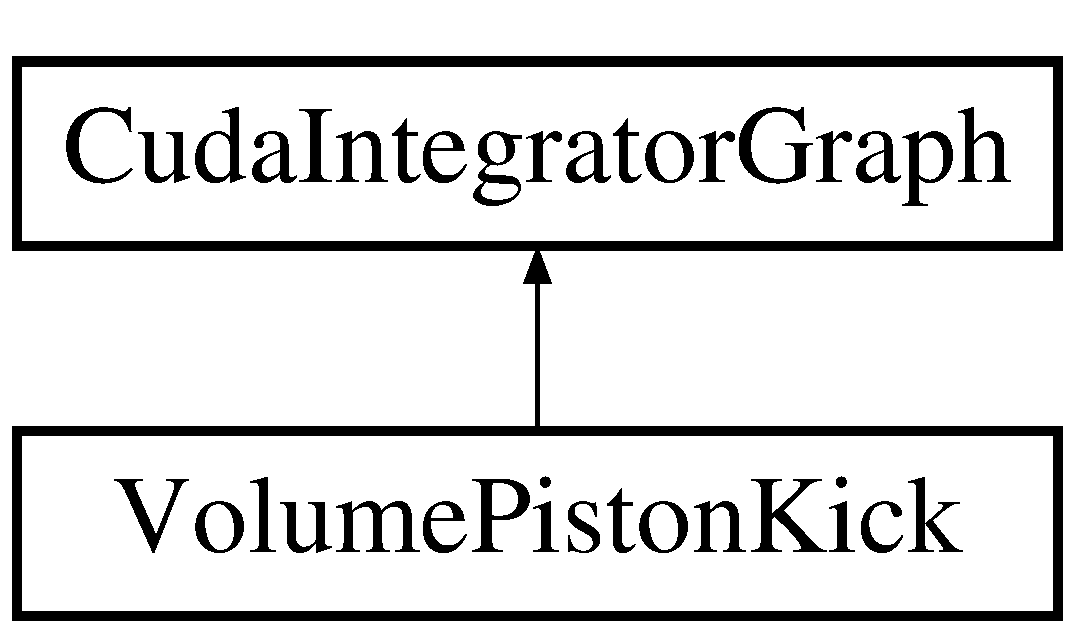
\includegraphics[height=2.000000cm]{classVolumePistonKick}
\end{center}
\end{figure}
\subsection*{Public Member Functions}
\begin{DoxyCompactItemize}
\item 
\hyperlink{classVolumePistonKick_adb5bdb93bb01be95881e4aeb5be3d3a7}{Volume\+Piston\+Kick} (const double3 $\ast$\+\_\+\+\_\+restrict\+\_\+\+\_\+ box, const double3 $\ast$old\+\_\+box\+\_\+dot, const double3 $\ast$\+\_\+\+\_\+restrict\+\_\+\+\_\+ virial, double3 $\ast$new\+\_\+box\+\_\+dot, double timestep, double piston\+\_\+mass)
\begin{DoxyCompactList}\small\item\em Create graph that updates the box time dirivative. \end{DoxyCompactList}\end{DoxyCompactItemize}
\subsection*{Additional Inherited Members}


\subsection{Detailed Description}
Create graph that updates the box time dirivative. 



\subsection{Constructor \& Destructor Documentation}
\hypertarget{classVolumePistonKick_adb5bdb93bb01be95881e4aeb5be3d3a7}{}\label{classVolumePistonKick_adb5bdb93bb01be95881e4aeb5be3d3a7} 
\index{Volume\+Piston\+Kick@{Volume\+Piston\+Kick}!Volume\+Piston\+Kick@{Volume\+Piston\+Kick}}
\index{Volume\+Piston\+Kick@{Volume\+Piston\+Kick}!Volume\+Piston\+Kick@{Volume\+Piston\+Kick}}
\subsubsection{\texorpdfstring{Volume\+Piston\+Kick()}{VolumePistonKick()}}
{\footnotesize\ttfamily Volume\+Piston\+Kick\+::\+Volume\+Piston\+Kick (\begin{DoxyParamCaption}\item[{const double3 $\ast$\+\_\+\+\_\+restrict\+\_\+\+\_\+}]{box,  }\item[{const double3 $\ast$}]{old\+\_\+box\+\_\+dot,  }\item[{const double3 $\ast$\+\_\+\+\_\+restrict\+\_\+\+\_\+}]{virial,  }\item[{double3 $\ast$}]{new\+\_\+box\+\_\+dot,  }\item[{double}]{timestep,  }\item[{double}]{piston\+\_\+mass }\end{DoxyParamCaption})}



Create graph that updates the box time dirivative. 


\begin{DoxyParams}{Parameters}
{\em box} & device pointer to box dimensions. \\
\hline
{\em old\+\_\+box\+\_\+dot} & device pointer to box time dirivative. \\
\hline
{\em virial} & device pointer to Corrected virial. \\
\hline
{\em new\+\_\+box\+\_\+dot} & device pointer to new box time dirivatives. \\
\hline
{\em timestep} & Time step. \\
\hline
{\em piston\+\_\+mass} & Piston mass, dimensions of mass/length$^\wedge$4. \\
\hline
\end{DoxyParams}


The documentation for this class was generated from the following file\+:\begin{DoxyCompactItemize}
\item 
/u/samar/\+Documents/git/chcuda/include/\hyperlink{VolumePistonKick_8h}{Volume\+Piston\+Kick.\+h}\end{DoxyCompactItemize}

\hypertarget{classVolumePistonLeapfrogDrift}{}\section{Volume\+Piston\+Leapfrog\+Drift Class Reference}
\label{classVolumePistonLeapfrogDrift}\index{Volume\+Piston\+Leapfrog\+Drift@{Volume\+Piston\+Leapfrog\+Drift}}


Create a graph that calculates the effect of constant pressure during the drift.  




{\ttfamily \#include $<$Volume\+Piston\+Leapfrog\+Drift.\+h$>$}

Inheritance diagram for Volume\+Piston\+Leapfrog\+Drift\+:\begin{figure}[H]
\begin{center}
\leavevmode
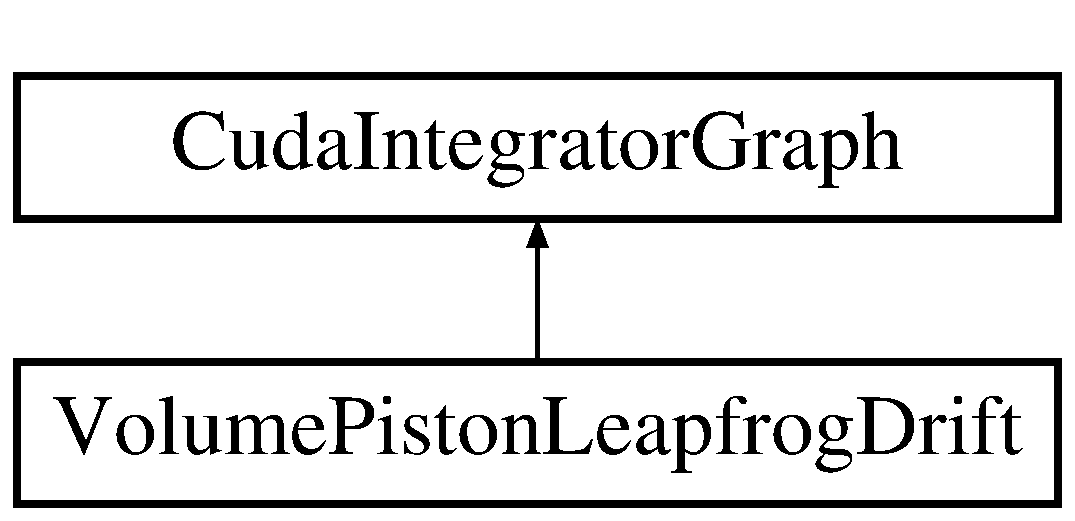
\includegraphics[height=2.000000cm]{classVolumePistonLeapfrogDrift}
\end{center}
\end{figure}
\subsection*{Public Member Functions}
\begin{DoxyCompactItemize}
\item 
\hyperlink{classVolumePistonLeapfrogDrift_a3872d09e073ce1b58d0a70beab29e487}{Volume\+Piston\+Leapfrog\+Drift} (const double3 $\ast$old\+\_\+com\+\_\+ke, const double3 $\ast$old\+\_\+box, const double3 $\ast$old\+\_\+box\+\_\+dot, double3 $\ast$new\+\_\+com\+\_\+ke, double3 $\ast$new\+\_\+box, double3 $\ast$new\+\_\+box\+\_\+dot, double3 $\ast$\+\_\+\+\_\+restrict\+\_\+\+\_\+ com\+\_\+momentum\+\_\+scale, double3 $\ast$\+\_\+\+\_\+restrict\+\_\+\+\_\+ com\+\_\+momentum\+\_\+prescale, double3 $\ast$\+\_\+\+\_\+restrict\+\_\+\+\_\+ com\+\_\+position\+\_\+prescale, double ref\+\_\+pressure, double timestep, double piston\+\_\+mass)
\begin{DoxyCompactList}\small\item\em Create a graph that calculates the effect of constant pressure. \end{DoxyCompactList}\end{DoxyCompactItemize}
\subsection*{Additional Inherited Members}


\subsection{Detailed Description}
Create a graph that calculates the effect of constant pressure during the drift. 

\subsection{Constructor \& Destructor Documentation}
\hypertarget{classVolumePistonLeapfrogDrift_a3872d09e073ce1b58d0a70beab29e487}{}\label{classVolumePistonLeapfrogDrift_a3872d09e073ce1b58d0a70beab29e487} 
\index{Volume\+Piston\+Leapfrog\+Drift@{Volume\+Piston\+Leapfrog\+Drift}!Volume\+Piston\+Leapfrog\+Drift@{Volume\+Piston\+Leapfrog\+Drift}}
\index{Volume\+Piston\+Leapfrog\+Drift@{Volume\+Piston\+Leapfrog\+Drift}!Volume\+Piston\+Leapfrog\+Drift@{Volume\+Piston\+Leapfrog\+Drift}}
\subsubsection{\texorpdfstring{Volume\+Piston\+Leapfrog\+Drift()}{VolumePistonLeapfrogDrift()}}
{\footnotesize\ttfamily Volume\+Piston\+Leapfrog\+Drift\+::\+Volume\+Piston\+Leapfrog\+Drift (\begin{DoxyParamCaption}\item[{const double3 $\ast$}]{old\+\_\+com\+\_\+ke,  }\item[{const double3 $\ast$}]{old\+\_\+box,  }\item[{const double3 $\ast$}]{old\+\_\+box\+\_\+dot,  }\item[{double3 $\ast$}]{new\+\_\+com\+\_\+ke,  }\item[{double3 $\ast$}]{new\+\_\+box,  }\item[{double3 $\ast$}]{new\+\_\+box\+\_\+dot,  }\item[{double3 $\ast$\+\_\+\+\_\+restrict\+\_\+\+\_\+}]{com\+\_\+momentum\+\_\+scale,  }\item[{double3 $\ast$\+\_\+\+\_\+restrict\+\_\+\+\_\+}]{com\+\_\+momentum\+\_\+prescale,  }\item[{double3 $\ast$\+\_\+\+\_\+restrict\+\_\+\+\_\+}]{com\+\_\+position\+\_\+prescale,  }\item[{double}]{ref\+\_\+pressure,  }\item[{double}]{timestep,  }\item[{double}]{piston\+\_\+mass }\end{DoxyParamCaption})}



Create a graph that calculates the effect of constant pressure. 

Piston Mass, dimensions of mass/length$^\wedge$4. 
\begin{DoxyParams}{Parameters}
{\em old\+\_\+com\+\_\+ke} & Device pointer to kinetic energy of pressure group momentums \\
\hline
{\em old\+\_\+box} & Device pointer to box lengths \\
\hline
{\em old\+\_\+box\+\_\+dot} & Device pointer to box length time dirivatives \\
\hline
{\em new\+\_\+com\+\_\+ke} & Device pointer to save post drift pressure group momentum kinetic energy \\
\hline
{\em new\+\_\+box} & Device pointer to save post drift box lengths \\
\hline
{\em new\+\_\+box\+\_\+dot} & Device pointer to save post drift box length time dirivatives \\
\hline
{\em com\+\_\+momentum\+\_\+scale} & Device pointer to final pressure group momentum scale. This is the total scale from predrift p group momentum to post drift p group momentum. \\
\hline
{\em com\+\_\+momentum\+\_\+prescale} & Device pointer to initial pressure group momentum scale. This is the scaleing of momentum that happens before the pressure group centers of mass are moved. \\
\hline
{\em com\+\_\+position\+\_\+prescale} & Device pointer to initial pressure group C\+OM scale. This is the scaling p group centers of mass before the are moved by their prescaled momenentums. \\
\hline
{\em ref\+\_\+pressure} & Reference pressure, units are not atms, it is SI compatible with other units. \\
\hline
{\em timestep} & Time step. \\
\hline
\end{DoxyParams}


The documentation for this class was generated from the following file\+:\begin{DoxyCompactItemize}
\item 
/u/samar/\+Documents/git/chcuda/include/\hyperlink{VolumePistonLeapfrogDrift_8h}{Volume\+Piston\+Leapfrog\+Drift.\+h}\end{DoxyCompactItemize}

\hypertarget{structxx14__t}{}\section{xx14\+\_\+t Struct Reference}
\label{structxx14__t}\index{xx14\+\_\+t@{xx14\+\_\+t}}
\subsection*{Public Member Functions}
\begin{DoxyCompactItemize}
\item 
\hypertarget{structxx14__t_aa0f2712a93d40d3ba7650f467d347c73}{}\label{structxx14__t_aa0f2712a93d40d3ba7650f467d347c73} 
void {\bfseries get\+Atoms} (std\+::vector$<$ int $>$ \&atoms)
\item 
\hypertarget{structxx14__t_a8d7ce42814d40fc5c2a9b2a1354a5867}{}\label{structxx14__t_a8d7ce42814d40fc5c2a9b2a1354a5867} 
void {\bfseries print\+Atoms} ()
\end{DoxyCompactItemize}
\subsection*{Static Public Member Functions}
\begin{DoxyCompactItemize}
\item 
\hypertarget{structxx14__t_a600980c6345b965f54dd27d2c9d6f49a}{}\label{structxx14__t_a600980c6345b965f54dd27d2c9d6f49a} 
static int {\bfseries type} ()
\item 
\hypertarget{structxx14__t_a7def9a6d5020153481b5b6d4863b9ab3}{}\label{structxx14__t_a7def9a6d5020153481b5b6d4863b9ab3} 
static int {\bfseries size} ()
\end{DoxyCompactItemize}
\subsection*{Public Attributes}
\begin{DoxyCompactItemize}
\item 
\hypertarget{structxx14__t_a3298a5a06f650b12a880fc0e13925273}{}\label{structxx14__t_a3298a5a06f650b12a880fc0e13925273} 
int {\bfseries i}
\item 
\hypertarget{structxx14__t_a63ef3505f70348c020b494698223813e}{}\label{structxx14__t_a63ef3505f70348c020b494698223813e} 
int {\bfseries j}
\end{DoxyCompactItemize}


The documentation for this struct was generated from the following file\+:\begin{DoxyCompactItemize}
\item 
/u/samar/\+Documents/git/chcuda/include/Bonded\+\_\+struct.\+h\end{DoxyCompactItemize}

\hypertarget{structxx14list__t}{}\section{xx14list\+\_\+t Struct Reference}
\label{structxx14list__t}\index{xx14list\+\_\+t@{xx14list\+\_\+t}}
\subsection*{Public Attributes}
\begin{DoxyCompactItemize}
\item 
\hypertarget{structxx14list__t_a8642f420ee0c2d7a5e4bc8892a7bfa6c}{}\label{structxx14list__t_a8642f420ee0c2d7a5e4bc8892a7bfa6c} 
int {\bfseries i}
\item 
\hypertarget{structxx14list__t_ad24b39dec5600fbd9840ddab92f05fab}{}\label{structxx14list__t_ad24b39dec5600fbd9840ddab92f05fab} 
int {\bfseries j}
\item 
\hypertarget{structxx14list__t_add18a6a25bc2821313835e733d9e789d}{}\label{structxx14list__t_add18a6a25bc2821313835e733d9e789d} 
int {\bfseries ishift}
\end{DoxyCompactItemize}


The documentation for this struct was generated from the following file\+:\begin{DoxyCompactItemize}
\item 
/u/samar/\+Documents/git/chcuda/include/Bonded\+\_\+struct.\+h\end{DoxyCompactItemize}

\hypertarget{classXYZ}{}\section{X\+YZ$<$ T $>$ Class Template Reference}
\label{classXYZ}\index{X\+Y\+Z$<$ T $>$@{X\+Y\+Z$<$ T $>$}}
Inheritance diagram for X\+YZ$<$ T $>$\+:\begin{figure}[H]
\begin{center}
\leavevmode
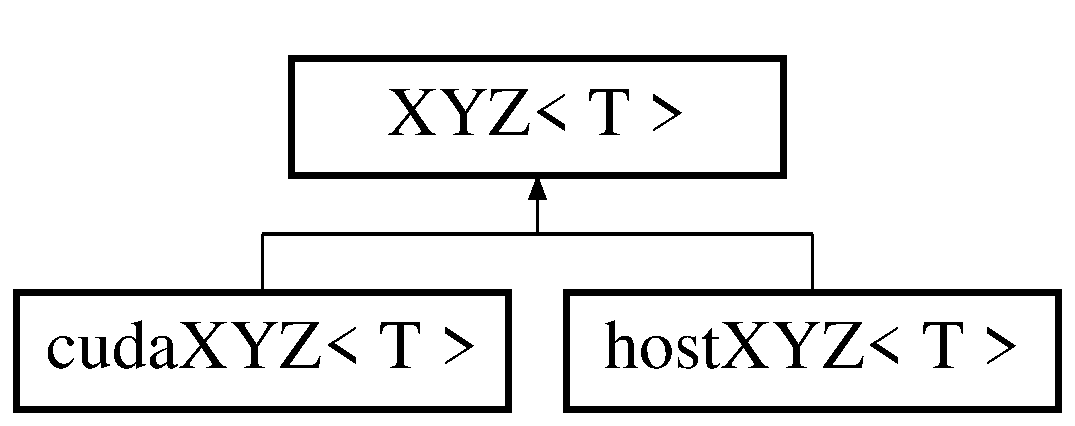
\includegraphics[height=2.000000cm]{classXYZ}
\end{center}
\end{figure}
\subsection*{Public Member Functions}
\begin{DoxyCompactItemize}
\item 
\hypertarget{classXYZ_a5abe4746ca1e21edd335eaf5fcba0375}{}\label{classXYZ_a5abe4746ca1e21edd335eaf5fcba0375} 
{\bfseries X\+YZ} (int size, int capacity, T $\ast$x, T $\ast$y, T $\ast$z)
\item 
\hypertarget{classXYZ_a967ddfe39739bd7715c83a01911ecfb4}{}\label{classXYZ_a967ddfe39739bd7715c83a01911ecfb4} 
{\footnotesize template$<$typename P $>$ }\\bool {\bfseries match} (const \hyperlink{classXYZ}{X\+YZ}$<$ P $>$ \&xyz)
\item 
\hypertarget{classXYZ_afcd15ec3cb6ad805d12e690c45f0f795}{}\label{classXYZ_afcd15ec3cb6ad805d12e690c45f0f795} 
void {\bfseries swap} (\hyperlink{classXYZ}{X\+YZ}$<$ T $>$ \&xyz)
\item 
\hypertarget{classXYZ_aaf4de0a9d062c01602c529274154186c}{}\label{classXYZ_aaf4de0a9d062c01602c529274154186c} 
virtual void {\bfseries realloc\+\_\+array} (T $\ast$$\ast$array, int $\ast$capacity, int size, float fac)=0
\item 
\hypertarget{classXYZ_a3fb6089d57851dbc8509e93b2dd2fb9a}{}\label{classXYZ_a3fb6089d57851dbc8509e93b2dd2fb9a} 
virtual void {\bfseries resize\+\_\+array} (T $\ast$$\ast$array, int $\ast$capacity, int size, int new\+\_\+size, float fac)=0
\item 
\hypertarget{classXYZ_a145ad0d3bc70e44181a0a7bc21207a47}{}\label{classXYZ_a145ad0d3bc70e44181a0a7bc21207a47} 
void {\bfseries resize} (int size, float fac=1.\+0f)
\item 
\hypertarget{classXYZ_a54b4a0b744457325060f2bcb016a0b1a}{}\label{classXYZ_a54b4a0b744457325060f2bcb016a0b1a} 
void {\bfseries realloc} (int size, float fac=1.\+0f)
\item 
\hypertarget{classXYZ_ac7d50ccb58b6e66c2eb05b83dcea6de4}{}\label{classXYZ_ac7d50ccb58b6e66c2eb05b83dcea6de4} 
virtual void {\bfseries get\+\_\+host\+\_\+xyz} (T $\ast$\&hx, T $\ast$\&hy, T $\ast$\&hz)=0
\item 
\hypertarget{classXYZ_a9eb21db264a140fe482a0a2d9ee31c4a}{}\label{classXYZ_a9eb21db264a140fe482a0a2d9ee31c4a} 
virtual void {\bfseries release\+\_\+host\+\_\+xyz} (T $\ast$\&hx, T $\ast$\&hy, T $\ast$\&hz)=0
\item 
\hypertarget{classXYZ_a7abeecd88fef6761a8a3da7f56474eec}{}\label{classXYZ_a7abeecd88fef6761a8a3da7f56474eec} 
void {\bfseries save} (const char $\ast$filename)
\item 
\hypertarget{classXYZ_a13044d0233ae303b19b0ff168a303ddc}{}\label{classXYZ_a13044d0233ae303b19b0ff168a303ddc} 
int {\bfseries size} ()
\item 
\hypertarget{classXYZ_a1b477643e1b5bbf1dced15bd6f5a56b1}{}\label{classXYZ_a1b477643e1b5bbf1dced15bd6f5a56b1} 
int {\bfseries size} () const
\item 
\hypertarget{classXYZ_a895142942cf937bbb8e16bec27cc132e}{}\label{classXYZ_a895142942cf937bbb8e16bec27cc132e} 
T $\ast$ {\bfseries x} ()
\item 
\hypertarget{classXYZ_a526423fc05e368999a519845d030a1bf}{}\label{classXYZ_a526423fc05e368999a519845d030a1bf} 
T $\ast$ {\bfseries y} ()
\item 
\hypertarget{classXYZ_abbbabb6bfdfcd0cfe01c1edec309ada8}{}\label{classXYZ_abbbabb6bfdfcd0cfe01c1edec309ada8} 
T $\ast$ {\bfseries z} ()
\item 
\hypertarget{classXYZ_add765a587a163c9f3fd213265021a738}{}\label{classXYZ_add765a587a163c9f3fd213265021a738} 
const T $\ast$ {\bfseries x} () const
\item 
\hypertarget{classXYZ_ae5b2be1c378c9c9914fcdf39a3f8dc9f}{}\label{classXYZ_ae5b2be1c378c9c9914fcdf39a3f8dc9f} 
const T $\ast$ {\bfseries y} () const
\item 
\hypertarget{classXYZ_a4bfe5e359c00cb49c99d75126fdc815f}{}\label{classXYZ_a4bfe5e359c00cb49c99d75126fdc815f} 
const T $\ast$ {\bfseries z} () const
\end{DoxyCompactItemize}
\subsection*{Protected Attributes}
\begin{DoxyCompactItemize}
\item 
\hypertarget{classXYZ_ae2f04dea56a813c97c9fb744bcd4bd5b}{}\label{classXYZ_ae2f04dea56a813c97c9fb744bcd4bd5b} 
int {\bfseries \+\_\+size}
\item 
\hypertarget{classXYZ_a99cf8beb331e391a1459eef5481b717a}{}\label{classXYZ_a99cf8beb331e391a1459eef5481b717a} 
int {\bfseries \+\_\+capacity}
\item 
\hypertarget{classXYZ_a03cce19bc05a4fc7a1b5d94e4a634d3e}{}\label{classXYZ_a03cce19bc05a4fc7a1b5d94e4a634d3e} 
T $\ast$ {\bfseries \+\_\+x}
\item 
\hypertarget{classXYZ_a4d78e4c4329cf83472189a031e3c5b7f}{}\label{classXYZ_a4d78e4c4329cf83472189a031e3c5b7f} 
T $\ast$ {\bfseries \+\_\+y}
\item 
\hypertarget{classXYZ_a75bab83bcc37b459f50d6e166860ffa7}{}\label{classXYZ_a75bab83bcc37b459f50d6e166860ffa7} 
T $\ast$ {\bfseries \+\_\+z}
\end{DoxyCompactItemize}


The documentation for this class was generated from the following file\+:\begin{DoxyCompactItemize}
\item 
/u/samar/\+Documents/git/chcuda/include/X\+Y\+Z.\+h\end{DoxyCompactItemize}

\hypertarget{classXYZQ}{}\section{X\+Y\+ZQ Class Reference}
\label{classXYZQ}\index{X\+Y\+ZQ@{X\+Y\+ZQ}}
\subsection*{Public Member Functions}
\begin{DoxyCompactItemize}
\item 
\hypertarget{classXYZQ_ac952868df5c6443d1bbbd1fdd1df48cf}{}\label{classXYZQ_ac952868df5c6443d1bbbd1fdd1df48cf} 
{\bfseries X\+Y\+ZQ} (int ncoord, int align=warpsize)
\item 
\hypertarget{classXYZQ_a14dba782e7793407478ad97bc62219ad}{}\label{classXYZQ_a14dba782e7793407478ad97bc62219ad} 
{\bfseries X\+Y\+ZQ} (const char $\ast$filename, int align=warpsize)
\item 
\hypertarget{classXYZQ_a8c52a476e3a374075572596a80baba7e}{}\label{classXYZQ_a8c52a476e3a374075572596a80baba7e} 
void {\bfseries set\+\_\+ncoord} (const int ncrd)
\item 
\hypertarget{classXYZQ_ab81af48d3d75d04ef5aee908c53f41cc}{}\label{classXYZQ_ab81af48d3d75d04ef5aee908c53f41cc} 
void {\bfseries realloc} (int ncoord\+\_\+new, float fac=1.\+0f)
\item 
\hypertarget{classXYZQ_a7d2d9d0066070c8d9ba650e4a952e7c1}{}\label{classXYZQ_a7d2d9d0066070c8d9ba650e4a952e7c1} 
void {\bfseries resize} (int ncoord\+\_\+new, float fac=1.\+0f)
\item 
\hypertarget{classXYZQ_aa429168e6b1fd60eb5eb3fe2994cbe73}{}\label{classXYZQ_aa429168e6b1fd60eb5eb3fe2994cbe73} 
void {\bfseries set\+\_\+xyzq} (int ncopy, const float4 $\ast$h\+\_\+xyzq, size\+\_\+t offset=0, cuda\+Stream\+\_\+t stream=0)
\item 
\hypertarget{classXYZQ_a64a2f7a04044cc0f98450db7b240b927}{}\label{classXYZQ_a64a2f7a04044cc0f98450db7b240b927} 
void {\bfseries set\+\_\+xyzq} (const \hyperlink{classcudaXYZ}{cuda\+X\+YZ}$<$ double $>$ \&coord, const float $\ast$q, cuda\+Stream\+\_\+t stream=0)
\item 
\hypertarget{classXYZQ_af930e9c6a44ec965b95972b5305ca3d4}{}\label{classXYZQ_af930e9c6a44ec965b95972b5305ca3d4} 
void {\bfseries set\+\_\+xyzq} (const \hyperlink{classcudaXYZ}{cuda\+X\+YZ}$<$ double $>$ \&coord, const float $\ast$q, const int $\ast$loc2glo, const float3 $\ast$xyz\+\_\+shift, const double boxx, const double boxy, const double boxz, cuda\+Stream\+\_\+t stream=0)
\item 
\hypertarget{classXYZQ_a71c8b38cb9597607937afbaf096ade8f}{}\label{classXYZQ_a71c8b38cb9597607937afbaf096ade8f} 
void {\bfseries set\+\_\+xyz} (const \hyperlink{classcudaXYZ}{cuda\+X\+YZ}$<$ double $>$ \&coord, cuda\+Stream\+\_\+t stream=0)
\item 
\hypertarget{classXYZQ_abebf79ca3e939e8c120683b664941ee1}{}\label{classXYZQ_abebf79ca3e939e8c120683b664941ee1} 
void {\bfseries set\+\_\+xyz} (const \hyperlink{classcudaXYZ}{cuda\+X\+YZ}$<$ double $>$ \&coord, const int start, const int end, const float3 $\ast$xyz\+\_\+shift, const double boxx, const double boxy, const double boxz, cuda\+Stream\+\_\+t stream=0)
\item 
\hypertarget{classXYZQ_a8c241380db8116c4ee51c250a5ac488e}{}\label{classXYZQ_a8c241380db8116c4ee51c250a5ac488e} 
bool {\bfseries compare} (\hyperlink{classXYZQ}{X\+Y\+ZQ} \&xyzq\+\_\+in, const double tol, double \&max\+\_\+diff)
\item 
\hypertarget{classXYZQ_a1f2e73eb1e3e584b938fb85b1a90338c}{}\label{classXYZQ_a1f2e73eb1e3e584b938fb85b1a90338c} 
void {\bfseries print} (const int start, const int end, std\+::ostream \&out)
\item 
\hypertarget{classXYZQ_aefb394e8c57e748cd45d1d1b11efff91}{}\label{classXYZQ_aefb394e8c57e748cd45d1d1b11efff91} 
void {\bfseries save} (const char $\ast$filename)
\item 
\hypertarget{classXYZQ_a4a83bb66b6eaa28b739b2e33bd63c0fb}{}\label{classXYZQ_a4a83bb66b6eaa28b739b2e33bd63c0fb} 
float4 $\ast$ {\bfseries get\+Device\+X\+Y\+ZQ} ()
\item 
\hypertarget{classXYZQ_a47a1039f97b2b58f9c87b06f07371e69}{}\label{classXYZQ_a47a1039f97b2b58f9c87b06f07371e69} 
void {\bfseries set\+Device\+X\+Y\+ZQ} (float4 $\ast$in)
\end{DoxyCompactItemize}
\subsection*{Public Attributes}
\begin{DoxyCompactItemize}
\item 
\hypertarget{classXYZQ_ab8e50a45c8fc45ce746b0ac80938d9db}{}\label{classXYZQ_ab8e50a45c8fc45ce746b0ac80938d9db} 
int {\bfseries align}
\item 
\hypertarget{classXYZQ_a96a7ca11354e5df5bfa344cd9e171e50}{}\label{classXYZQ_a96a7ca11354e5df5bfa344cd9e171e50} 
int {\bfseries ncoord}
\item 
\hypertarget{classXYZQ_a70df9f6ea3ec361b9efc297bcfdbfa6e}{}\label{classXYZQ_a70df9f6ea3ec361b9efc297bcfdbfa6e} 
int {\bfseries xyzq\+\_\+len}
\item 
\hypertarget{classXYZQ_ab24be1814bde15c39f437fab575d03f7}{}\label{classXYZQ_ab24be1814bde15c39f437fab575d03f7} 
float4 $\ast$ {\bfseries xyzq}
\end{DoxyCompactItemize}


The documentation for this class was generated from the following file\+:\begin{DoxyCompactItemize}
\item 
/u/samar/\+Documents/git/chcuda/include/X\+Y\+Z\+Q.\+h\end{DoxyCompactItemize}

\hypertarget{structZoneParam__t}{}\section{Zone\+Param\+\_\+t Struct Reference}
\label{structZoneParam__t}\index{Zone\+Param\+\_\+t@{Zone\+Param\+\_\+t}}
\subsection*{Public Attributes}
\begin{DoxyCompactItemize}
\item 
\hypertarget{structZoneParam__t_abff7685c795f227d3b907808f618f08d}{}\label{structZoneParam__t_abff7685c795f227d3b907808f618f08d} 
float3 {\bfseries min\+\_\+xyz}
\item 
\hypertarget{structZoneParam__t_ab4e04e5ddf111f093211fab26a52e9a3}{}\label{structZoneParam__t_ab4e04e5ddf111f093211fab26a52e9a3} 
float3 {\bfseries max\+\_\+xyz}
\item 
\hypertarget{structZoneParam__t_a1f2333a7146984d06e6536f6fa98c06d}{}\label{structZoneParam__t_a1f2333a7146984d06e6536f6fa98c06d} 
int {\bfseries ncellx}
\item 
\hypertarget{structZoneParam__t_af1076c526a40ed39204659fd28245534}{}\label{structZoneParam__t_af1076c526a40ed39204659fd28245534} 
int {\bfseries ncelly}
\item 
\hypertarget{structZoneParam__t_ae8cf566a5e1b3a1eaa0406ae74c9c7c6}{}\label{structZoneParam__t_ae8cf566a5e1b3a1eaa0406ae74c9c7c6} 
int {\bfseries ncellz\+\_\+max}
\item 
\hypertarget{structZoneParam__t_a90832f4b7094aa160a20a5a8ca288cde}{}\label{structZoneParam__t_a90832f4b7094aa160a20a5a8ca288cde} 
float {\bfseries celldx}
\item 
\hypertarget{structZoneParam__t_aa40ade23f3d19fd25e26540a0f00d666}{}\label{structZoneParam__t_aa40ade23f3d19fd25e26540a0f00d666} 
float {\bfseries celldy}
\item 
\hypertarget{structZoneParam__t_ac56f85238b3bef7020434e4517d0be81}{}\label{structZoneParam__t_ac56f85238b3bef7020434e4517d0be81} 
float {\bfseries celldz\+\_\+min}
\item 
\hypertarget{structZoneParam__t_aed894049e776cea3eabe3bef84aa0ae6}{}\label{structZoneParam__t_aed894049e776cea3eabe3bef84aa0ae6} 
float {\bfseries inv\+\_\+celldx}
\item 
\hypertarget{structZoneParam__t_a8b6441fbe8252a2844e20d9c4cc1df0d}{}\label{structZoneParam__t_a8b6441fbe8252a2844e20d9c4cc1df0d} 
float {\bfseries inv\+\_\+celldy}
\item 
\hypertarget{structZoneParam__t_a05a7fbb2a7d4ec6c91c7235b9053eff0}{}\label{structZoneParam__t_a05a7fbb2a7d4ec6c91c7235b9053eff0} 
int {\bfseries n\+\_\+int\+\_\+zone}
\item 
\hypertarget{structZoneParam__t_a04677d1510bdff690da67d24014a3c12}{}\label{structZoneParam__t_a04677d1510bdff690da67d24014a3c12} 
int {\bfseries int\+\_\+zone} \mbox{[}max\+Num\+Int\+Zone\mbox{]}
\item 
\hypertarget{structZoneParam__t_a47892717e754ba68520edd16fb4a76cd}{}\label{structZoneParam__t_a47892717e754ba68520edd16fb4a76cd} 
int {\bfseries zone\+\_\+col}
\item 
\hypertarget{structZoneParam__t_a74728e7abeb4f6b9c45a88257f0d79b4}{}\label{structZoneParam__t_a74728e7abeb4f6b9c45a88257f0d79b4} 
int {\bfseries ncoord}
\end{DoxyCompactItemize}


The documentation for this struct was generated from the following file\+:\begin{DoxyCompactItemize}
\item 
/u/samar/\+Documents/git/chcuda/include/Cuda\+Neighbor\+List\+Struct.\+h\end{DoxyCompactItemize}

\chapter{File Documentation}
\hypertarget{AtomVelocityKick_8h}{}\section{/u/samar/\+Documents/git/chcuda/include/\+Atom\+Velocity\+Kick.h File Reference}
\label{AtomVelocityKick_8h}\index{/u/samar/\+Documents/git/chcuda/include/\+Atom\+Velocity\+Kick.\+h@{/u/samar/\+Documents/git/chcuda/include/\+Atom\+Velocity\+Kick.\+h}}


Graphs and kernels to update the atom velocities by a force.  


{\ttfamily \#include $<$cuda\+\_\+runtime.\+h$>$}\newline
{\ttfamily \#include $<$cuda\+\_\+utils.\+h$>$}\newline
{\ttfamily \#include $<$stdint.\+h$>$}\newline
{\ttfamily \#include $<$Cuda\+Integrator\+Graph.\+h$>$}\newline
{\ttfamily \#include $<$array$>$}\newline
\subsection*{Functions}
\begin{DoxyCompactItemize}
\item 
\+\_\+\+\_\+global\+\_\+\+\_\+ void \hyperlink{AtomVelocityKick_8h_a1cc1954157f2b939d9debcdd8b8f7052}{atom\+Velocity\+Kick\+Simple\+Kernel} (const double4 $\ast$old\+\_\+vel\+\_\+mass, const double4 $\ast$\+\_\+\+\_\+restrict\+\_\+\+\_\+ force\+\_\+invmass, double $\ast$new\+\_\+vel\+\_\+mass, int num\+Atoms, double timestep)
\begin{DoxyCompactList}\small\item\em Update atom velocities based on their invese mass, their force, and the timestep. \end{DoxyCompactList}\item 
class \hyperlink{AtomVelocityKick_8h_aac6e80352e9c23dcacae463cfccf1aeb}{Atom\+Velocity\+Kick} (public \+:Atom\+Velocity\+Kick(const double4 $\ast$old\+\_\+vel\+\_\+mass, const double4 $\ast$\+\_\+\+\_\+restrict\+\_\+\+\_\+ force\+\_\+invmass, double $\ast$new\+\_\+vel\+\_\+mass, int num\+Atoms, double timestep);private \+:void initialize\+Graph(void);cuda\+Kernel\+Node\+Params myparams;std\+::array$<$ void $\ast$, 8 $>$ kernel\+Args;cuda\+Graph\+Node\+\_\+t mynode;const double4 $\ast$old\+\_\+vel\+\_\+mass;const double4 $\ast$\+\_\+\+\_\+restrict\+\_\+\+\_\+ force\+\_\+invmass;double $\ast$new\+\_\+vel\+\_\+mass;int num\+Atoms;double timestep)
\begin{DoxyCompactList}\small\item\em Create a graph that updates the atom velocities based on the forces. \end{DoxyCompactList}\end{DoxyCompactItemize}


\subsection{Detailed Description}
Graphs and kernels to update the atom velocities by a force. 

\begin{DoxyAuthor}{Author}
Nathan Zimmerberg (\href{mailto:nhz2@cornell.edu}{\tt nhz2@cornell.\+edu}) 
\end{DoxyAuthor}
\begin{DoxyDate}{Date}

\end{DoxyDate}


\subsection{Function Documentation}
\hypertarget{AtomVelocityKick_8h_aac6e80352e9c23dcacae463cfccf1aeb}{}\label{AtomVelocityKick_8h_aac6e80352e9c23dcacae463cfccf1aeb} 
\index{Atom\+Velocity\+Kick.\+h@{Atom\+Velocity\+Kick.\+h}!Atom\+Velocity\+Kick@{Atom\+Velocity\+Kick}}
\index{Atom\+Velocity\+Kick@{Atom\+Velocity\+Kick}!Atom\+Velocity\+Kick.\+h@{Atom\+Velocity\+Kick.\+h}}
\subsubsection{\texorpdfstring{Atom\+Velocity\+Kick()}{AtomVelocityKick()}}
{\footnotesize\ttfamily class Atom\+Velocity\+Kick (\begin{DoxyParamCaption}\item[{public \+:Atom\+Velocity\+Kick(const double4 $\ast$old\+\_\+vel\+\_\+mass, const double4 $\ast$\+\_\+\+\_\+restrict\+\_\+\+\_\+ force\+\_\+invmass, double $\ast$new\+\_\+vel\+\_\+mass, int num\+Atoms, double timestep);private \+:void initialize\+Graph(void);cuda\+Kernel\+Node\+Params myparams;std\+::array$<$ void $\ast$, 8 $>$ kernel\+Args;cuda\+Graph\+Node\+\_\+t mynode;const double4 $\ast$old\+\_\+vel\+\_\+mass;const double4 $\ast$\+\_\+\+\_\+restrict\+\_\+\+\_\+ force\+\_\+invmass;double $\ast$new\+\_\+vel\+\_\+mass;int num\+Atoms;double}]{timestep }\end{DoxyParamCaption})}



Create a graph that updates the atom velocities based on the forces. 


\begin{DoxyParams}{Parameters}
{\em timestep} & Device pointer to atom velocity and mass. Device pointer to force and inverse mass of atoms. Device pointer to updated atom velocities. Number of atoms. Time step. \\
\hline
\end{DoxyParams}
\hypertarget{AtomVelocityKick_8h_a1cc1954157f2b939d9debcdd8b8f7052}{}\label{AtomVelocityKick_8h_a1cc1954157f2b939d9debcdd8b8f7052} 
\index{Atom\+Velocity\+Kick.\+h@{Atom\+Velocity\+Kick.\+h}!atom\+Velocity\+Kick\+Simple\+Kernel@{atom\+Velocity\+Kick\+Simple\+Kernel}}
\index{atom\+Velocity\+Kick\+Simple\+Kernel@{atom\+Velocity\+Kick\+Simple\+Kernel}!Atom\+Velocity\+Kick.\+h@{Atom\+Velocity\+Kick.\+h}}
\subsubsection{\texorpdfstring{atom\+Velocity\+Kick\+Simple\+Kernel()}{atomVelocityKickSimpleKernel()}}
{\footnotesize\ttfamily \+\_\+\+\_\+global\+\_\+\+\_\+ void atom\+Velocity\+Kick\+Simple\+Kernel (\begin{DoxyParamCaption}\item[{const double4 $\ast$}]{old\+\_\+vel\+\_\+mass,  }\item[{const double4 $\ast$\+\_\+\+\_\+restrict\+\_\+\+\_\+}]{force\+\_\+invmass,  }\item[{double $\ast$}]{new\+\_\+vel\+\_\+mass,  }\item[{int}]{num\+Atoms,  }\item[{double}]{timestep }\end{DoxyParamCaption})}



Update atom velocities based on their invese mass, their force, and the timestep. 


\begin{DoxyParams}{Parameters}
{\em old\+\_\+vel\+\_\+mass} & Device pointer to atom velocity and mass. \\
\hline
{\em force\+\_\+invmass} & Device pointer to force and inverse mass of atoms. \\
\hline
{\em new\+\_\+vel\+\_\+mass} & Device pointer to updated atom velocities. \\
\hline
{\em num\+Atoms} & Number of atoms. \\
\hline
{\em timestep} & Time step. \\
\hline
\end{DoxyParams}

\hypertarget{ConstantPressurePostDrift_8h}{}\section{/u/samar/\+Documents/git/chcuda/include/\+Constant\+Pressure\+Post\+Drift.h File Reference}
\label{ConstantPressurePostDrift_8h}\index{/u/samar/\+Documents/git/chcuda/include/\+Constant\+Pressure\+Post\+Drift.\+h@{/u/samar/\+Documents/git/chcuda/include/\+Constant\+Pressure\+Post\+Drift.\+h}}


Recombine com coordinates and relative coordinates for next force calculation.  


{\ttfamily \#include $<$cuda\+\_\+runtime.\+h$>$}\newline
{\ttfamily \#include $<$cuda\+\_\+utils.\+h$>$}\newline
{\ttfamily \#include $<$stdint.\+h$>$}\newline
{\ttfamily \#include $<$array$>$}\newline
{\ttfamily \#include $<$Pressure\+Groups\+Util.\+h$>$}\newline
{\ttfamily \#include $<$Cuda\+Integrator\+Graph.\+h$>$}\newline
\subsection*{Classes}
\begin{DoxyCompactItemize}
\item 
class \hyperlink{classConstantPressurePostDrift}{Constant\+Pressure\+Post\+Drift}
\begin{DoxyCompactList}\small\item\em Create a graph that gets absolute coords back from relative coords. \end{DoxyCompactList}\end{DoxyCompactItemize}
\subsection*{Functions}
\begin{DoxyCompactItemize}
\item 
\+\_\+\+\_\+global\+\_\+\+\_\+ void \hyperlink{ConstantPressurePostDrift_8h_a6218690bebf935fca185f6b1be8c03ee}{constant\+Pressure\+Post\+Drift\+Simple\+Kernel} (const double4 $\ast$\+\_\+\+\_\+restrict\+\_\+\+\_\+ relative\+\_\+xyzq, const double4 $\ast$\+\_\+\+\_\+restrict\+\_\+\+\_\+ relative\+\_\+vel\+\_\+mass, const \hyperlink{structComID__t}{Com\+I\+D\+\_\+t} $\ast$\+\_\+\+\_\+restrict\+\_\+\+\_\+ com\+\_\+ids, const double4 $\ast$\+\_\+\+\_\+restrict\+\_\+\+\_\+ com\+\_\+momentum\+\_\+invmass, double4 $\ast$\+\_\+\+\_\+restrict\+\_\+\+\_\+ absolute\+\_\+xyzq, double4 $\ast$\+\_\+\+\_\+restrict\+\_\+\+\_\+ absolute\+\_\+vel\+\_\+mass, const int $\ast$sorted\+\_\+atomids, int num\+Groups)
\begin{DoxyCompactList}\small\item\em Recombine center of mass coordinates and relative coordinates to get absolute coordinates. \end{DoxyCompactList}\end{DoxyCompactItemize}


\subsection{Detailed Description}
Recombine com coordinates and relative coordinates for next force calculation. 

\begin{DoxyAuthor}{Author}
Nathan Zimmerberg (\href{mailto:nhz2@cornell.edu}{\tt nhz2@cornell.\+edu}) 
\end{DoxyAuthor}
\begin{DoxyDate}{Date}

\end{DoxyDate}


\subsection{Function Documentation}
\hypertarget{ConstantPressurePostDrift_8h_a6218690bebf935fca185f6b1be8c03ee}{}\label{ConstantPressurePostDrift_8h_a6218690bebf935fca185f6b1be8c03ee} 
\index{Constant\+Pressure\+Post\+Drift.\+h@{Constant\+Pressure\+Post\+Drift.\+h}!constant\+Pressure\+Post\+Drift\+Simple\+Kernel@{constant\+Pressure\+Post\+Drift\+Simple\+Kernel}}
\index{constant\+Pressure\+Post\+Drift\+Simple\+Kernel@{constant\+Pressure\+Post\+Drift\+Simple\+Kernel}!Constant\+Pressure\+Post\+Drift.\+h@{Constant\+Pressure\+Post\+Drift.\+h}}
\subsubsection{\texorpdfstring{constant\+Pressure\+Post\+Drift\+Simple\+Kernel()}{constantPressurePostDriftSimpleKernel()}}
{\footnotesize\ttfamily \+\_\+\+\_\+global\+\_\+\+\_\+ void constant\+Pressure\+Post\+Drift\+Simple\+Kernel (\begin{DoxyParamCaption}\item[{const double4 $\ast$\+\_\+\+\_\+restrict\+\_\+\+\_\+}]{relative\+\_\+xyzq,  }\item[{const double4 $\ast$\+\_\+\+\_\+restrict\+\_\+\+\_\+}]{relative\+\_\+vel\+\_\+mass,  }\item[{const \hyperlink{structComID__t}{Com\+I\+D\+\_\+t} $\ast$\+\_\+\+\_\+restrict\+\_\+\+\_\+}]{com\+\_\+ids,  }\item[{const double4 $\ast$\+\_\+\+\_\+restrict\+\_\+\+\_\+}]{com\+\_\+momentum\+\_\+invmass,  }\item[{double4 $\ast$\+\_\+\+\_\+restrict\+\_\+\+\_\+}]{absolute\+\_\+xyzq,  }\item[{double4 $\ast$\+\_\+\+\_\+restrict\+\_\+\+\_\+}]{absolute\+\_\+vel\+\_\+mass,  }\item[{const int $\ast$}]{sorted\+\_\+atomids,  }\item[{int}]{num\+Groups }\end{DoxyParamCaption})}



Recombine center of mass coordinates and relative coordinates to get absolute coordinates. 


\begin{DoxyParams}{Parameters}
{\em relative\+\_\+xyzq} & The device pointer to the array of atom positions relative to the center of mass of their pressure group. \\
\hline
{\em relative\+\_\+vel\+\_\+mass} & The device pointer to the array of relative velocity and mass of every atom. \\
\hline
{\em com\+\_\+ids} & The device pointer to the array of the position of the center of mass of each pressure group, and the atoms that are in the group. \\
\hline
{\em com\+\_\+momentum\+\_\+invmass} & The device pointer to the array of the group net momentums and inverse masses. \\
\hline
{\em absolute\+\_\+xyzq} & The device pointer to the array of absolute atom positions. \\
\hline
{\em absolute\+\_\+vel\+\_\+mass} & The device pointer to the array of absolute velocity and mass of every atom. \\
\hline
{\em sorted\+\_\+atomids} & Array of all atom ids sorted by pressure group. \\
\hline
{\em num\+Groups} & number of groups. \\
\hline
\end{DoxyParams}

\hypertarget{ConstantPressurePrepareDrift_8h}{}\section{/u/samar/\+Documents/git/chcuda/include/\+Constant\+Pressure\+Prepare\+Drift.h File Reference}
\label{ConstantPressurePrepareDrift_8h}\index{/u/samar/\+Documents/git/chcuda/include/\+Constant\+Pressure\+Prepare\+Drift.\+h@{/u/samar/\+Documents/git/chcuda/include/\+Constant\+Pressure\+Prepare\+Drift.\+h}}


Class and kernels for Cuda graphs to prepare for the drift stage.  


{\ttfamily \#include $<$cuda\+\_\+runtime.\+h$>$}\newline
{\ttfamily \#include $<$cuda\+\_\+utils.\+h$>$}\newline
{\ttfamily \#include $<$stdint.\+h$>$}\newline
{\ttfamily \#include $<$Cuda\+Integrator\+Graph.\+h$>$}\newline
{\ttfamily \#include $<$array$>$}\newline
{\ttfamily \#include $<$Pressure\+Groups\+Util.\+h$>$}\newline
\subsection*{Classes}
\begin{DoxyCompactItemize}
\item 
class \hyperlink{classConstantPressurePrepareDrift}{Constant\+Pressure\+Prepare\+Drift}
\begin{DoxyCompactList}\small\item\em Create a graph that calculates the net momentums, center of masses(\+C\+O\+M), relative coordinates to the C\+O\+Ms, internal momentums, and kinetic energies from the C\+OM motion, and kinetic energies from the internal motions. \end{DoxyCompactList}\end{DoxyCompactItemize}
\subsection*{Functions}
\begin{DoxyCompactItemize}
\item 
\+\_\+\+\_\+global\+\_\+\+\_\+ void \hyperlink{ConstantPressurePrepareDrift_8h_a40df3f08b3c2013a6f26fc4d3c2d4142}{constant\+Pressure\+Prepare\+Drift\+Simple\+Kernel} (const double4 $\ast$\+\_\+\+\_\+restrict\+\_\+\+\_\+ absolute\+\_\+vel\+\_\+mass, const double4 $\ast$\+\_\+\+\_\+restrict\+\_\+\+\_\+ absolute\+\_\+xyzq, double4 $\ast$\+\_\+\+\_\+restrict\+\_\+\+\_\+ relative\+\_\+xyzq, double4 $\ast$\+\_\+\+\_\+restrict\+\_\+\+\_\+ relative\+\_\+vel\+\_\+mass, \hyperlink{structComID__t}{Com\+I\+D\+\_\+t} $\ast$\+\_\+\+\_\+restrict\+\_\+\+\_\+ com\+\_\+ids, double4 $\ast$\+\_\+\+\_\+restrict\+\_\+\+\_\+ com\+\_\+momentum\+\_\+invmass, double3 $\ast$\+\_\+\+\_\+restrict\+\_\+\+\_\+ com\+\_\+kinetic\+\_\+energy, double $\ast$\+\_\+\+\_\+restrict\+\_\+\+\_\+ total\+\_\+kinetic\+\_\+energy, const int $\ast$sorted\+\_\+atomids, int num\+Groups)
\begin{DoxyCompactList}\small\item\em calculate the net momentums, center of masses(\+C\+O\+M), relative coordinates to the C\+O\+Ms, internal momentums, and kinetic energies from the C\+OM motion, and kinetic energies from the internal motions. \end{DoxyCompactList}\end{DoxyCompactItemize}


\subsection{Detailed Description}
Class and kernels for Cuda graphs to prepare for the drift stage. 

\begin{DoxyAuthor}{Author}
Nathan Zimmerberg (\href{mailto:nhz2@cornell.edu}{\tt nhz2@cornell.\+edu}) 
\end{DoxyAuthor}
\begin{DoxyDate}{Date}

\end{DoxyDate}
The graph will calculate the net momentums, center of masses(\+C\+O\+M), relative coordinates to the C\+O\+Ms, internal momentums, and kinetic energies from the C\+OM motion, and kinetic energies from the internal motions. 

\subsection{Function Documentation}
\hypertarget{ConstantPressurePrepareDrift_8h_a40df3f08b3c2013a6f26fc4d3c2d4142}{}\label{ConstantPressurePrepareDrift_8h_a40df3f08b3c2013a6f26fc4d3c2d4142} 
\index{Constant\+Pressure\+Prepare\+Drift.\+h@{Constant\+Pressure\+Prepare\+Drift.\+h}!constant\+Pressure\+Prepare\+Drift\+Simple\+Kernel@{constant\+Pressure\+Prepare\+Drift\+Simple\+Kernel}}
\index{constant\+Pressure\+Prepare\+Drift\+Simple\+Kernel@{constant\+Pressure\+Prepare\+Drift\+Simple\+Kernel}!Constant\+Pressure\+Prepare\+Drift.\+h@{Constant\+Pressure\+Prepare\+Drift.\+h}}
\subsubsection{\texorpdfstring{constant\+Pressure\+Prepare\+Drift\+Simple\+Kernel()}{constantPressurePrepareDriftSimpleKernel()}}
{\footnotesize\ttfamily \+\_\+\+\_\+global\+\_\+\+\_\+ void constant\+Pressure\+Prepare\+Drift\+Simple\+Kernel (\begin{DoxyParamCaption}\item[{const double4 $\ast$\+\_\+\+\_\+restrict\+\_\+\+\_\+}]{absolute\+\_\+vel\+\_\+mass,  }\item[{const double4 $\ast$\+\_\+\+\_\+restrict\+\_\+\+\_\+}]{absolute\+\_\+xyzq,  }\item[{double4 $\ast$\+\_\+\+\_\+restrict\+\_\+\+\_\+}]{relative\+\_\+xyzq,  }\item[{double4 $\ast$\+\_\+\+\_\+restrict\+\_\+\+\_\+}]{relative\+\_\+vel\+\_\+mass,  }\item[{\hyperlink{structComID__t}{Com\+I\+D\+\_\+t} $\ast$\+\_\+\+\_\+restrict\+\_\+\+\_\+}]{com\+\_\+ids,  }\item[{double4 $\ast$\+\_\+\+\_\+restrict\+\_\+\+\_\+}]{com\+\_\+momentum\+\_\+invmass,  }\item[{double3 $\ast$\+\_\+\+\_\+restrict\+\_\+\+\_\+}]{com\+\_\+kinetic\+\_\+energy,  }\item[{double $\ast$\+\_\+\+\_\+restrict\+\_\+\+\_\+}]{total\+\_\+kinetic\+\_\+energy,  }\item[{const int $\ast$}]{sorted\+\_\+atomids,  }\item[{int}]{num\+Groups }\end{DoxyParamCaption})}



calculate the net momentums, center of masses(\+C\+O\+M), relative coordinates to the C\+O\+Ms, internal momentums, and kinetic energies from the C\+OM motion, and kinetic energies from the internal motions. 


\begin{DoxyParams}{Parameters}
{\em absolute\+\_\+vel\+\_\+mass} & The device pointer to the array of absolute velocity and mass of every atom. \\
\hline
{\em absolute\+\_\+xyzq} & The device pointer to the array of absolute atom positions. \\
\hline
{\em relative\+\_\+xyzq} & The device pointer to the array of atom positions relative to the center of mass of their pressure group. \\
\hline
{\em relative\+\_\+vel\+\_\+mass} & The device pointer to the array of relative velocity and mass of every atom. \\
\hline
{\em com\+\_\+ids} & The device pointer to the array of the position of the center of mass of each pressure group, and the atoms that are in the group. \\
\hline
{\em com\+\_\+momentum\+\_\+invmass} & The device pointer to the array of the group net momentums and inverse masses. \\
\hline
{\em com\+\_\+kinetic\+\_\+energy} & The xx,yy, and zz components of the groups center of mass kinetic energy. \\
\hline
{\em total\+\_\+kinetic\+\_\+energy} & The total kinetic energy. \\
\hline
{\em sorted\+\_\+atomids} & Array of all atom ids sorted by pressure group. \\
\hline
{\em num\+Groups} & number of groups. \\
\hline
\end{DoxyParams}

\hypertarget{CudaIntegratorGraph_8h}{}\section{/u/samar/\+Documents/git/chcuda/include/\+Cuda\+Integrator\+Graph.h File Reference}
\label{CudaIntegratorGraph_8h}\index{/u/samar/\+Documents/git/chcuda/include/\+Cuda\+Integrator\+Graph.\+h@{/u/samar/\+Documents/git/chcuda/include/\+Cuda\+Integrator\+Graph.\+h}}


Base class for cuda integrator graphs and some utilities for making nodes from kernals easily.  


{\ttfamily \#include $<$cuda\+\_\+runtime.\+h$>$}\newline
{\ttfamily \#include $<$cuda\+\_\+utils.\+h$>$}\newline
\subsection*{Classes}
\begin{DoxyCompactItemize}
\item 
class \hyperlink{classCudaIntegratorGraph}{Cuda\+Integrator\+Graph}
\begin{DoxyCompactList}\small\item\em Base class for other cuda integrator classes. \end{DoxyCompactList}\end{DoxyCompactItemize}


\subsection{Detailed Description}
Base class for cuda integrator graphs and some utilities for making nodes from kernals easily. 

\begin{DoxyAuthor}{Author}
Nathan Zimmerberg (\href{mailto:nhz2@cornell.edu}{\tt nhz2@cornell.\+edu}) 
\end{DoxyAuthor}
\begin{DoxyDate}{Date}
07/16/2019 
\end{DoxyDate}

\hypertarget{CudaSimulationContext_8h}{}\section{/u/samar/\+Documents/git/chcuda/include/\+Cuda\+Simulation\+Context.h File Reference}
\label{CudaSimulationContext_8h}\index{/u/samar/\+Documents/git/chcuda/include/\+Cuda\+Simulation\+Context.\+h@{/u/samar/\+Documents/git/chcuda/include/\+Cuda\+Simulation\+Context.\+h}}
{\ttfamily \#include $<$memory$>$}\newline
{\ttfamily \#include $<$vector$>$}\newline
{\ttfamily \#include \char`\"{}Cuda\+Container.\+h\char`\"{}}\newline
{\ttfamily \#include \char`\"{}Cuda\+Bonded\+Force.\+h\char`\"{}}\newline
{\ttfamily \#include \char`\"{}Cuda\+Energy\+Virial.\+h\char`\"{}}\newline
{\ttfamily \#include \char`\"{}Cuda\+P\+M\+E\+Direct\+Force.\+h\char`\"{}}\newline
{\ttfamily \#include \char`\"{}Cuda\+Top\+Excl.\+h\char`\"{}}\newline
{\ttfamily \#include \char`\"{}Cuda\+Neighbor\+List\+Build.\+h\char`\"{}}\newline
{\ttfamily \#include \char`\"{}Cuda\+Neighbor\+List.\+h\char`\"{}}\newline
{\ttfamily \#include \char`\"{}cuda\+\_\+utils.\+h\char`\"{}}\newline
{\ttfamily \#include \char`\"{}Force.\+h\char`\"{}}\newline
{\ttfamily \#include \char`\"{}X\+Y\+Z\+Q.\+h\char`\"{}}\newline
{\ttfamily \#include \char`\"{}Cuda\+Domdec\+Recip.\+h\char`\"{}}\newline
{\ttfamily \#include $<$Volume\+Piston.\+h$>$}\newline
{\ttfamily \#include $<$random\+\_\+utils.\+h$>$}\newline
\subsection*{Classes}
\begin{DoxyCompactItemize}
\item 
struct \hyperlink{structH__DVector}{H\+\_\+\+D\+Vector$<$ T $>$}
\item 
class \hyperlink{classCudaSimulationContext}{Cuda\+Simulation\+Context}
\end{DoxyCompactItemize}
\subsection*{Typedefs}
\begin{DoxyCompactItemize}
\item 
\hypertarget{CudaSimulationContext_8h_a1b277d5ccb37c54911599215cb5e53d6}{}\label{CudaSimulationContext_8h_a1b277d5ccb37c54911599215cb5e53d6} 
typedef float {\bfseries CT}
\item 
\hypertarget{CudaSimulationContext_8h_afc45571e93be91381a76351286b146f2}{}\label{CudaSimulationContext_8h_afc45571e93be91381a76351286b146f2} 
typedef float4 {\bfseries C\+T4}
\end{DoxyCompactItemize}
\subsection*{Enumerations}
\begin{DoxyCompactItemize}
\item 
\hypertarget{CudaSimulationContext_8h_a64aa06d157e8ef0dc6c6eb00aec6ebf8}{}\label{CudaSimulationContext_8h_a64aa06d157e8ef0dc6c6eb00aec6ebf8} 
enum {\bfseries P\+BC} \{ {\bfseries P1}, 
{\bfseries P21}
 \}
\end{DoxyCompactItemize}

\hypertarget{KineticEnergyGraph_8h}{}\section{/u/samar/\+Documents/git/chcuda/include/\+Kinetic\+Energy\+Graph.h File Reference}
\label{KineticEnergyGraph_8h}\index{/u/samar/\+Documents/git/chcuda/include/\+Kinetic\+Energy\+Graph.\+h@{/u/samar/\+Documents/git/chcuda/include/\+Kinetic\+Energy\+Graph.\+h}}


Class and kernels to calculate the total kinetic energy.  


{\ttfamily \#include $<$cuda\+\_\+runtime.\+h$>$}\newline
{\ttfamily \#include $<$cuda\+\_\+utils.\+h$>$}\newline
{\ttfamily \#include $<$stdint.\+h$>$}\newline
{\ttfamily \#include $<$Cuda\+Integrator\+Graph.\+h$>$}\newline
{\ttfamily \#include $<$array$>$}\newline
\subsection*{Classes}
\begin{DoxyCompactItemize}
\item 
class \hyperlink{classKineticEnergyGraph}{Kinetic\+Energy\+Graph}
\begin{DoxyCompactList}\small\item\em Create a graph that calculates the kinetic energy. \end{DoxyCompactList}\end{DoxyCompactItemize}
\subsection*{Functions}
\begin{DoxyCompactItemize}
\item 
\+\_\+\+\_\+global\+\_\+\+\_\+ void \hyperlink{KineticEnergyGraph_8h_a5b86eabaf4a77a475f390b51659757ee}{kinetic\+Energy\+Simple\+Kernel} (const double4 $\ast$\+\_\+\+\_\+restrict\+\_\+\+\_\+ vel\+\_\+mass, double $\ast$\+\_\+\+\_\+restrict\+\_\+\+\_\+ total\+\_\+kinetic\+\_\+energy, int num\+Atoms)
\begin{DoxyCompactList}\small\item\em calculate the total kinetic energy \end{DoxyCompactList}\end{DoxyCompactItemize}


\subsection{Detailed Description}
Class and kernels to calculate the total kinetic energy. 

\begin{DoxyAuthor}{Author}
Nathan Zimmerberg (\href{mailto:nhz2@cornell.edu}{\tt nhz2@cornell.\+edu}) 
\end{DoxyAuthor}
\begin{DoxyDate}{Date}

\end{DoxyDate}


\subsection{Function Documentation}
\hypertarget{KineticEnergyGraph_8h_a5b86eabaf4a77a475f390b51659757ee}{}\label{KineticEnergyGraph_8h_a5b86eabaf4a77a475f390b51659757ee} 
\index{Kinetic\+Energy\+Graph.\+h@{Kinetic\+Energy\+Graph.\+h}!kinetic\+Energy\+Simple\+Kernel@{kinetic\+Energy\+Simple\+Kernel}}
\index{kinetic\+Energy\+Simple\+Kernel@{kinetic\+Energy\+Simple\+Kernel}!Kinetic\+Energy\+Graph.\+h@{Kinetic\+Energy\+Graph.\+h}}
\subsubsection{\texorpdfstring{kinetic\+Energy\+Simple\+Kernel()}{kineticEnergySimpleKernel()}}
{\footnotesize\ttfamily \+\_\+\+\_\+global\+\_\+\+\_\+ void kinetic\+Energy\+Simple\+Kernel (\begin{DoxyParamCaption}\item[{const double4 $\ast$\+\_\+\+\_\+restrict\+\_\+\+\_\+}]{vel\+\_\+mass,  }\item[{double $\ast$\+\_\+\+\_\+restrict\+\_\+\+\_\+}]{total\+\_\+kinetic\+\_\+energy,  }\item[{int}]{num\+Atoms }\end{DoxyParamCaption})}



calculate the total kinetic energy 


\begin{DoxyParams}{Parameters}
{\em vel\+\_\+mass} & The device pointer to the array of velocity and mass of every atom. \\
\hline
{\em total\+\_\+kinetic\+\_\+energy} & The total kinetic energy. \\
\hline
{\em num\+Atoms} & number of atoms. \\
\hline
\end{DoxyParams}

\hypertarget{PressureGroupDrift_8h}{}\section{/u/samar/\+Documents/git/chcuda/include/\+Pressure\+Group\+Drift.h File Reference}
\label{PressureGroupDrift_8h}\index{/u/samar/\+Documents/git/chcuda/include/\+Pressure\+Group\+Drift.\+h@{/u/samar/\+Documents/git/chcuda/include/\+Pressure\+Group\+Drift.\+h}}


Classes and kernels to move and scale the centers of mass and net momentums of each pressure group.  


{\ttfamily \#include $<$cuda\+\_\+runtime.\+h$>$}\newline
{\ttfamily \#include $<$cuda\+\_\+utils.\+h$>$}\newline
{\ttfamily \#include $<$stdint.\+h$>$}\newline
{\ttfamily \#include $<$Cuda\+Integrator\+Graph.\+h$>$}\newline
{\ttfamily \#include $<$Pressure\+Groups\+Util.\+h$>$}\newline
\subsection*{Functions}
\begin{DoxyCompactItemize}
\item 
\+\_\+\+\_\+global\+\_\+\+\_\+ void \hyperlink{PressureGroupDrift_8h_a17750f308f6b38f528643d66f56dfc9c}{scale\+Drift\+Simple\+Kernel} (const double3 $\ast$\+\_\+\+\_\+restrict\+\_\+\+\_\+ momentum\+\_\+scale, const double3 $\ast$\+\_\+\+\_\+restrict\+\_\+\+\_\+ momentum\+\_\+prescale, const double3 $\ast$\+\_\+\+\_\+restrict\+\_\+\+\_\+ position\+\_\+prescale, const double4 $\ast$old\+\_\+momentum\+\_\+invmass, const double4 $\ast$old\+\_\+xyzq, double4 $\ast$new\+\_\+momentum\+\_\+invmass, double4 $\ast$new\+\_\+xyzq, double timestep, int num)
\begin{DoxyCompactList}\small\item\em calculate new positions and momentums with scaling. \end{DoxyCompactList}\end{DoxyCompactItemize}


\subsection{Detailed Description}
Classes and kernels to move and scale the centers of mass and net momentums of each pressure group. 

\begin{DoxyAuthor}{Author}
Nathan Zimmerberg (\href{mailto:nhz2@cornell.edu}{\tt nhz2@cornell.\+edu}) 
\end{DoxyAuthor}
\begin{DoxyDate}{Date}

\end{DoxyDate}


\subsection{Function Documentation}
\hypertarget{PressureGroupDrift_8h_a17750f308f6b38f528643d66f56dfc9c}{}\label{PressureGroupDrift_8h_a17750f308f6b38f528643d66f56dfc9c} 
\index{Pressure\+Group\+Drift.\+h@{Pressure\+Group\+Drift.\+h}!scale\+Drift\+Simple\+Kernel@{scale\+Drift\+Simple\+Kernel}}
\index{scale\+Drift\+Simple\+Kernel@{scale\+Drift\+Simple\+Kernel}!Pressure\+Group\+Drift.\+h@{Pressure\+Group\+Drift.\+h}}
\subsubsection{\texorpdfstring{scale\+Drift\+Simple\+Kernel()}{scaleDriftSimpleKernel()}}
{\footnotesize\ttfamily \+\_\+\+\_\+global\+\_\+\+\_\+ void scale\+Drift\+Simple\+Kernel (\begin{DoxyParamCaption}\item[{const double3 $\ast$\+\_\+\+\_\+restrict\+\_\+\+\_\+}]{momentum\+\_\+scale,  }\item[{const double3 $\ast$\+\_\+\+\_\+restrict\+\_\+\+\_\+}]{momentum\+\_\+prescale,  }\item[{const double3 $\ast$\+\_\+\+\_\+restrict\+\_\+\+\_\+}]{position\+\_\+prescale,  }\item[{const double4 $\ast$}]{old\+\_\+momentum\+\_\+invmass,  }\item[{const double4 $\ast$}]{old\+\_\+xyzq,  }\item[{double4 $\ast$}]{new\+\_\+momentum\+\_\+invmass,  }\item[{double4 $\ast$}]{new\+\_\+xyzq,  }\item[{double}]{timestep,  }\item[{int}]{num }\end{DoxyParamCaption})}



calculate new positions and momentums with scaling. 

new\+\_\+momentum= old\+\_\+momentum$\ast$momentum\+\_\+scale new\+\_\+xyz= old\+\_\+xyz$\ast$position\+\_\+prescale+timestep$\ast$momentum$\ast$invmass$\ast$momentum\+\_\+prescale 
\begin{DoxyParams}{Parameters}
{\em momentum\+\_\+scale} & Device Pointer to total scaling of momentum. \\
\hline
{\em momentum\+\_\+prescale} & Device pointer to momentum scaling for position update. \\
\hline
{\em position\+\_\+prescale} & Device pointer to position scaling before moving. \\
\hline
{\em old\+\_\+momentum\+\_\+invmass} & Device pointer to array of momentums and inverse masses. \\
\hline
{\em old\+\_\+xyzq} & Device pointer to array of positions. \\
\hline
{\em new\+\_\+momentum\+\_\+invmass} & Device pointer to array of new momentums, and invers masses. \\
\hline
{\em new\+\_\+xyzq} & Device pointer to array of new positions. \\
\hline
{\em timestep} & time step. \\
\hline
{\em num} & number of elements in the arrays. \\
\hline
\end{DoxyParams}

\hypertarget{PressureGroupMomentumUpdate_8h}{}\section{/u/samar/\+Documents/git/chcuda/include/\+Pressure\+Group\+Momentum\+Update.h File Reference}
\label{PressureGroupMomentumUpdate_8h}\index{/u/samar/\+Documents/git/chcuda/include/\+Pressure\+Group\+Momentum\+Update.\+h@{/u/samar/\+Documents/git/chcuda/include/\+Pressure\+Group\+Momentum\+Update.\+h}}


The class and kernels to update the net momentums of the pressure groups.  


{\ttfamily \#include $<$cuda\+\_\+runtime.\+h$>$}\newline
{\ttfamily \#include $<$cuda\+\_\+utils.\+h$>$}\newline
{\ttfamily \#include $<$stdint.\+h$>$}\newline
{\ttfamily \#include $<$Cuda\+Integrator\+Graph.\+h$>$}\newline
{\ttfamily \#include $<$array$>$}\newline
\subsection*{Classes}
\begin{DoxyCompactItemize}
\item 
struct \hyperlink{structAtomIdList__t}{Atom\+Id\+List\+\_\+t}
\begin{DoxyCompactList}\small\item\em Type to store an array of atom ids. \end{DoxyCompactList}\item 
class \hyperlink{classPressureGroupMomentumUpdate}{Pressure\+Group\+Momentum\+Update}
\begin{DoxyCompactList}\small\item\em Create a graph that gets the net force on each pressure group and calc the new momentum. \end{DoxyCompactList}\end{DoxyCompactItemize}
\subsection*{Functions}
\begin{DoxyCompactItemize}
\item 
\+\_\+\+\_\+global\+\_\+\+\_\+ void \hyperlink{PressureGroupMomentumUpdate_8h_a30db48890cf03041635806727cba5e84}{pressure\+Group\+Momentum\+Update\+Simple\+Kernel} (const double $\ast$\+\_\+\+\_\+restrict\+\_\+\+\_\+ forcex, const double $\ast$\+\_\+\+\_\+restrict\+\_\+\+\_\+ forcey, const double $\ast$\+\_\+\+\_\+restrict\+\_\+\+\_\+ forcez, const double4 $\ast$old\+\_\+momentum\+\_\+invmass, double4 $\ast$new\+\_\+momentum\+\_\+invmass, const \hyperlink{structAtomIdList__t}{Atom\+Id\+List\+\_\+t} $\ast$\+\_\+\+\_\+restrict\+\_\+\+\_\+ group\+\_\+atom\+\_\+ids, double timestep, int num\+Groups)
\begin{DoxyCompactList}\small\item\em Set the new momentums to the old momentums + the net force$\ast$ timestep. \end{DoxyCompactList}\end{DoxyCompactItemize}


\subsection{Detailed Description}
The class and kernels to update the net momentums of the pressure groups. 

\begin{DoxyAuthor}{Author}
Nathan Zimmerberg (\href{mailto:nhz2@cornell.edu}{\tt nhz2@cornell.\+edu}) 
\end{DoxyAuthor}
\begin{DoxyDate}{Date}

\end{DoxyDate}


\subsection{Function Documentation}
\hypertarget{PressureGroupMomentumUpdate_8h_a30db48890cf03041635806727cba5e84}{}\label{PressureGroupMomentumUpdate_8h_a30db48890cf03041635806727cba5e84} 
\index{Pressure\+Group\+Momentum\+Update.\+h@{Pressure\+Group\+Momentum\+Update.\+h}!pressure\+Group\+Momentum\+Update\+Simple\+Kernel@{pressure\+Group\+Momentum\+Update\+Simple\+Kernel}}
\index{pressure\+Group\+Momentum\+Update\+Simple\+Kernel@{pressure\+Group\+Momentum\+Update\+Simple\+Kernel}!Pressure\+Group\+Momentum\+Update.\+h@{Pressure\+Group\+Momentum\+Update.\+h}}
\subsubsection{\texorpdfstring{pressure\+Group\+Momentum\+Update\+Simple\+Kernel()}{pressureGroupMomentumUpdateSimpleKernel()}}
{\footnotesize\ttfamily \+\_\+\+\_\+global\+\_\+\+\_\+ void pressure\+Group\+Momentum\+Update\+Simple\+Kernel (\begin{DoxyParamCaption}\item[{const double $\ast$\+\_\+\+\_\+restrict\+\_\+\+\_\+}]{forcex,  }\item[{const double $\ast$\+\_\+\+\_\+restrict\+\_\+\+\_\+}]{forcey,  }\item[{const double $\ast$\+\_\+\+\_\+restrict\+\_\+\+\_\+}]{forcez,  }\item[{const double4 $\ast$}]{old\+\_\+momentum\+\_\+invmass,  }\item[{double4 $\ast$}]{new\+\_\+momentum\+\_\+invmass,  }\item[{const \hyperlink{structAtomIdList__t}{Atom\+Id\+List\+\_\+t} $\ast$\+\_\+\+\_\+restrict\+\_\+\+\_\+}]{group\+\_\+atom\+\_\+ids,  }\item[{double}]{timestep,  }\item[{int}]{num\+Groups }\end{DoxyParamCaption})}



Set the new momentums to the old momentums + the net force$\ast$ timestep. 


\hypertarget{PressureGroupScaleDrift_8h}{}\section{/u/samar/\+Documents/git/chcuda/include/\+Pressure\+Group\+Scale\+Drift.h File Reference}
\label{PressureGroupScaleDrift_8h}\index{/u/samar/\+Documents/git/chcuda/include/\+Pressure\+Group\+Scale\+Drift.\+h@{/u/samar/\+Documents/git/chcuda/include/\+Pressure\+Group\+Scale\+Drift.\+h}}


Classes and kernels to move and scale the centers of mass and net momentums of each pressure group.  


{\ttfamily \#include $<$cuda\+\_\+runtime.\+h$>$}\newline
{\ttfamily \#include $<$cuda\+\_\+utils.\+h$>$}\newline
{\ttfamily \#include $<$stdint.\+h$>$}\newline
{\ttfamily \#include $<$array$>$}\newline
{\ttfamily \#include $<$Cuda\+Integrator\+Graph.\+h$>$}\newline
{\ttfamily \#include $<$Pressure\+Groups\+Util.\+h$>$}\newline
{\ttfamily \#include $<$nv\+Vector.\+h$>$}\newline
\subsection*{Classes}
\begin{DoxyCompactItemize}
\item 
class \hyperlink{classPressureGroupScaleDrift}{Pressure\+Group\+Scale\+Drift}
\begin{DoxyCompactList}\small\item\em Create a graph that calculates the new pressure group center positions and momentums with scaling. \end{DoxyCompactList}\end{DoxyCompactItemize}
\subsection*{Functions}
\begin{DoxyCompactItemize}
\item 
\+\_\+\+\_\+global\+\_\+\+\_\+ void \hyperlink{PressureGroupScaleDrift_8h_a17750f308f6b38f528643d66f56dfc9c}{scale\+Drift\+Simple\+Kernel} (const double3 $\ast$\+\_\+\+\_\+restrict\+\_\+\+\_\+ momentum\+\_\+scale, const double3 $\ast$\+\_\+\+\_\+restrict\+\_\+\+\_\+ momentum\+\_\+prescale, const double3 $\ast$\+\_\+\+\_\+restrict\+\_\+\+\_\+ position\+\_\+prescale, const double4 $\ast$old\+\_\+momentum\+\_\+invmass, const double4 $\ast$old\+\_\+xyzq, double4 $\ast$new\+\_\+momentum\+\_\+invmass, double4 $\ast$new\+\_\+xyzq, double timestep, int num)
\begin{DoxyCompactList}\small\item\em calculate new positions and momentums with scaling. \end{DoxyCompactList}\end{DoxyCompactItemize}


\subsection{Detailed Description}
Classes and kernels to move and scale the centers of mass and net momentums of each pressure group. 

\begin{DoxyAuthor}{Author}
Nathan Zimmerberg (\href{mailto:nhz2@cornell.edu}{\tt nhz2@cornell.\+edu}) 
\end{DoxyAuthor}
\begin{DoxyDate}{Date}

\end{DoxyDate}


\subsection{Function Documentation}
\hypertarget{PressureGroupScaleDrift_8h_a17750f308f6b38f528643d66f56dfc9c}{}\label{PressureGroupScaleDrift_8h_a17750f308f6b38f528643d66f56dfc9c} 
\index{Pressure\+Group\+Scale\+Drift.\+h@{Pressure\+Group\+Scale\+Drift.\+h}!scale\+Drift\+Simple\+Kernel@{scale\+Drift\+Simple\+Kernel}}
\index{scale\+Drift\+Simple\+Kernel@{scale\+Drift\+Simple\+Kernel}!Pressure\+Group\+Scale\+Drift.\+h@{Pressure\+Group\+Scale\+Drift.\+h}}
\subsubsection{\texorpdfstring{scale\+Drift\+Simple\+Kernel()}{scaleDriftSimpleKernel()}}
{\footnotesize\ttfamily \+\_\+\+\_\+global\+\_\+\+\_\+ void scale\+Drift\+Simple\+Kernel (\begin{DoxyParamCaption}\item[{const double3 $\ast$\+\_\+\+\_\+restrict\+\_\+\+\_\+}]{momentum\+\_\+scale,  }\item[{const double3 $\ast$\+\_\+\+\_\+restrict\+\_\+\+\_\+}]{momentum\+\_\+prescale,  }\item[{const double3 $\ast$\+\_\+\+\_\+restrict\+\_\+\+\_\+}]{position\+\_\+prescale,  }\item[{const double4 $\ast$}]{old\+\_\+momentum\+\_\+invmass,  }\item[{const double4 $\ast$}]{old\+\_\+xyzq,  }\item[{double4 $\ast$}]{new\+\_\+momentum\+\_\+invmass,  }\item[{double4 $\ast$}]{new\+\_\+xyzq,  }\item[{double}]{timestep,  }\item[{int}]{num }\end{DoxyParamCaption})}



calculate new positions and momentums with scaling. 

new\+\_\+momentum= old\+\_\+momentum$\ast$momentum\+\_\+scale new\+\_\+xyz= old\+\_\+xyz$\ast$position\+\_\+prescale+timestep$\ast$momentum$\ast$invmass$\ast$momentum\+\_\+prescale 
\begin{DoxyParams}{Parameters}
{\em momentum\+\_\+scale} & Device Pointer to total scaling of momentum. \\
\hline
{\em momentum\+\_\+prescale} & Device pointer to momentum scaling for position update. \\
\hline
{\em position\+\_\+prescale} & Device pointer to position scaling before moving. \\
\hline
{\em old\+\_\+momentum\+\_\+invmass} & Device pointer to array of momentums and inverse masses. \\
\hline
{\em old\+\_\+xyzq} & Device pointer to array of positions. \\
\hline
{\em new\+\_\+momentum\+\_\+invmass} & Device pointer to array of new momentums, and invers masses. \\
\hline
{\em new\+\_\+xyzq} & Device pointer to array of new positions. \\
\hline
{\em timestep} & time step. \\
\hline
{\em num} & number of elements in the arrays. \\
\hline
\end{DoxyParams}

\hypertarget{PressureGroupsUtil_8h}{}\section{/u/samar/\+Documents/git/chcuda/include/\+Pressure\+Groups\+Util.h File Reference}
\label{PressureGroupsUtil_8h}\index{/u/samar/\+Documents/git/chcuda/include/\+Pressure\+Groups\+Util.\+h@{/u/samar/\+Documents/git/chcuda/include/\+Pressure\+Groups\+Util.\+h}}


Utility structs and inline functions for N\+PT.  


\subsection*{Classes}
\begin{DoxyCompactItemize}
\item 
struct \hyperlink{structAtomIdList__t}{Atom\+Id\+List\+\_\+t}
\begin{DoxyCompactList}\small\item\em Type to store an array of atom ids. \end{DoxyCompactList}\item 
struct \hyperlink{structComID__t}{Com\+I\+D\+\_\+t}
\begin{DoxyCompactList}\small\item\em Type to store the center of mass of a group, and its atom id list. \end{DoxyCompactList}\end{DoxyCompactItemize}


\subsection{Detailed Description}
Utility structs and inline functions for N\+PT. 

\begin{DoxyAuthor}{Author}
Nathan Zimmerberg (\href{mailto:nhz2@cornell.edu}{\tt nhz2@cornell.\+edu}) 
\end{DoxyAuthor}
\begin{DoxyDate}{Date}

\end{DoxyDate}

\hypertarget{PressureGroupVirial_8h}{}\section{/u/samar/\+Documents/git/chcuda/include/\+Pressure\+Group\+Virial.h File Reference}
\label{PressureGroupVirial_8h}\index{/u/samar/\+Documents/git/chcuda/include/\+Pressure\+Group\+Virial.\+h@{/u/samar/\+Documents/git/chcuda/include/\+Pressure\+Group\+Virial.\+h}}


Functions and kernals to Calculate the correction to the virial to account for pressure groups.  


{\ttfamily \#include $<$array$>$}\newline
{\ttfamily \#include $<$stdint.\+h$>$}\newline
{\ttfamily \#include $<$cuda\+\_\+runtime.\+h$>$}\newline
{\ttfamily \#include $<$cuda\+\_\+utils.\+h$>$}\newline
{\ttfamily \#include $<$Cuda\+Integrator\+Graph.\+h$>$}\newline
\subsection*{Classes}
\begin{DoxyCompactItemize}
\item 
class \hyperlink{classPressureGroupVirialGraph}{Pressure\+Group\+Virial\+Graph}
\begin{DoxyCompactList}\small\item\em Creates a graph that calculates the virial correction for pressure groups. \end{DoxyCompactList}\end{DoxyCompactItemize}
\subsection*{Functions}
\begin{DoxyCompactItemize}
\item 
\hypertarget{PressureGroupVirial_8h_a0ddf6c2589840bc12e0f3d642fba8d0d}{}\label{PressureGroupVirial_8h_a0ddf6c2589840bc12e0f3d642fba8d0d} 
\+\_\+\+\_\+global\+\_\+\+\_\+ void \hyperlink{PressureGroupVirial_8h_a0ddf6c2589840bc12e0f3d642fba8d0d}{pressure\+Group\+Virial\+Simple\+Kernel} (const double $\ast$\+\_\+\+\_\+restrict\+\_\+\+\_\+ forcex, const double $\ast$\+\_\+\+\_\+restrict\+\_\+\+\_\+ forcey, const double $\ast$\+\_\+\+\_\+restrict\+\_\+\+\_\+ forcez, const double $\ast$\+\_\+\+\_\+restrict\+\_\+\+\_\+ relative\+\_\+coordsx, const double $\ast$\+\_\+\+\_\+restrict\+\_\+\+\_\+ relative\+\_\+coordsy, const double $\ast$\+\_\+\+\_\+restrict\+\_\+\+\_\+ relative\+\_\+coordsz, int num\+Atoms, double3 $\ast$\+\_\+\+\_\+restrict\+\_\+\+\_\+ virial)
\begin{DoxyCompactList}\small\item\em Result is an array of the sum of the element wise product of each force and its position. \end{DoxyCompactList}\end{DoxyCompactItemize}


\subsection{Detailed Description}
Functions and kernals to Calculate the correction to the virial to account for pressure groups. 

\begin{DoxyAuthor}{Author}
Nathan Zimmerberg (\href{mailto:nhz2@cornell.edu}{\tt nhz2@cornell.\+edu}) 
\end{DoxyAuthor}
\begin{DoxyDate}{Date}
17 Jul 2019 
\end{DoxyDate}

\hypertarget{PressureGroupVirialGraph_8h}{}\section{/u/samar/\+Documents/git/chcuda/include/\+Pressure\+Group\+Virial\+Graph.h File Reference}
\label{PressureGroupVirialGraph_8h}\index{/u/samar/\+Documents/git/chcuda/include/\+Pressure\+Group\+Virial\+Graph.\+h@{/u/samar/\+Documents/git/chcuda/include/\+Pressure\+Group\+Virial\+Graph.\+h}}


Functions and kernals to Calculate the correction to the virial to account for pressure groups.  


{\ttfamily \#include $<$array$>$}\newline
{\ttfamily \#include $<$stdint.\+h$>$}\newline
{\ttfamily \#include $<$cuda\+\_\+runtime.\+h$>$}\newline
{\ttfamily \#include $<$cuda\+\_\+utils.\+h$>$}\newline
{\ttfamily \#include $<$Cuda\+Integrator\+Graph.\+h$>$}\newline
\subsection*{Classes}
\begin{DoxyCompactItemize}
\item 
class \hyperlink{classPressureGroupVirialGraph}{Pressure\+Group\+Virial\+Graph}
\begin{DoxyCompactList}\small\item\em Creates a graph that calculates the virial correction for pressure groups. \end{DoxyCompactList}\end{DoxyCompactItemize}
\subsection*{Functions}
\begin{DoxyCompactItemize}
\item 
\hypertarget{PressureGroupVirialGraph_8h_a0ddf6c2589840bc12e0f3d642fba8d0d}{}\label{PressureGroupVirialGraph_8h_a0ddf6c2589840bc12e0f3d642fba8d0d} 
\+\_\+\+\_\+global\+\_\+\+\_\+ void \hyperlink{PressureGroupVirialGraph_8h_a0ddf6c2589840bc12e0f3d642fba8d0d}{pressure\+Group\+Virial\+Simple\+Kernel} (const double $\ast$\+\_\+\+\_\+restrict\+\_\+\+\_\+ forcex, const double $\ast$\+\_\+\+\_\+restrict\+\_\+\+\_\+ forcey, const double $\ast$\+\_\+\+\_\+restrict\+\_\+\+\_\+ forcez, const double $\ast$\+\_\+\+\_\+restrict\+\_\+\+\_\+ relative\+\_\+coordsx, const double $\ast$\+\_\+\+\_\+restrict\+\_\+\+\_\+ relative\+\_\+coordsy, const double $\ast$\+\_\+\+\_\+restrict\+\_\+\+\_\+ relative\+\_\+coordsz, int num\+Atoms, double3 $\ast$\+\_\+\+\_\+restrict\+\_\+\+\_\+ virial)
\begin{DoxyCompactList}\small\item\em virial gets the sum of the element wise product of each force and its position. \end{DoxyCompactList}\end{DoxyCompactItemize}


\subsection{Detailed Description}
Functions and kernals to Calculate the correction to the virial to account for pressure groups. 

\begin{DoxyAuthor}{Author}
Nathan Zimmerberg (\href{mailto:nhz2@cornell.edu}{\tt nhz2@cornell.\+edu}) 
\end{DoxyAuthor}
\begin{DoxyDate}{Date}
17 Jul 2019 
\end{DoxyDate}

\hypertarget{PrintEnergiesGraph_8h}{}\section{/u/samar/\+Documents/git/chcuda/include/\+Print\+Energies\+Graph.h File Reference}
\label{PrintEnergiesGraph_8h}\index{/u/samar/\+Documents/git/chcuda/include/\+Print\+Energies\+Graph.\+h@{/u/samar/\+Documents/git/chcuda/include/\+Print\+Energies\+Graph.\+h}}


graphs and kernels to print the kinetic energy.  


{\ttfamily \#include $<$cuda\+\_\+runtime.\+h$>$}\newline
{\ttfamily \#include $<$cuda\+\_\+utils.\+h$>$}\newline
{\ttfamily \#include $<$stdint.\+h$>$}\newline
{\ttfamily \#include $<$array$>$}\newline
{\ttfamily \#include $<$Cuda\+Integrator\+Graph.\+h$>$}\newline
{\ttfamily \#include $<$Volume\+Piston.\+h$>$}\newline
\subsection*{Classes}
\begin{DoxyCompactItemize}
\item 
struct \hyperlink{structPrintEnergiesGraphInputs}{Print\+Energies\+Graph\+Inputs}
\begin{DoxyCompactList}\small\item\em input for the graph that prints out the components of the total system energy. \end{DoxyCompactList}\item 
class \hyperlink{classPrintEnergiesGraph}{Print\+Energies\+Graph}
\begin{DoxyCompactList}\small\item\em Create a graph to print the system energies. \end{DoxyCompactList}\end{DoxyCompactItemize}
\subsection*{Functions}
\begin{DoxyCompactItemize}
\item 
\+\_\+\+\_\+global\+\_\+\+\_\+ void \hyperlink{PrintEnergiesGraph_8h_a9b7572a78f4ffe9016a2b11285146cb5}{Print\+Energies\+Graph\+Kernel} (\hyperlink{structPrintEnergiesGraphInputs}{Print\+Energies\+Graph\+Inputs} in)
\begin{DoxyCompactList}\small\item\em Print out Energies. \end{DoxyCompactList}\end{DoxyCompactItemize}


\subsection{Detailed Description}
graphs and kernels to print the kinetic energy. 

\begin{DoxyAuthor}{Author}
Nathan Zimmerberg (\href{mailto:nhz2@cornell.edu}{\tt nhz2@cornell.\+edu}) 
\end{DoxyAuthor}
\begin{DoxyDate}{Date}

\end{DoxyDate}


\subsection{Function Documentation}
\hypertarget{PrintEnergiesGraph_8h_a9b7572a78f4ffe9016a2b11285146cb5}{}\label{PrintEnergiesGraph_8h_a9b7572a78f4ffe9016a2b11285146cb5} 
\index{Print\+Energies\+Graph.\+h@{Print\+Energies\+Graph.\+h}!Print\+Energies\+Graph\+Kernel@{Print\+Energies\+Graph\+Kernel}}
\index{Print\+Energies\+Graph\+Kernel@{Print\+Energies\+Graph\+Kernel}!Print\+Energies\+Graph.\+h@{Print\+Energies\+Graph.\+h}}
\subsubsection{\texorpdfstring{Print\+Energies\+Graph\+Kernel()}{PrintEnergiesGraphKernel()}}
{\footnotesize\ttfamily \+\_\+\+\_\+global\+\_\+\+\_\+ void Print\+Energies\+Graph\+Kernel (\begin{DoxyParamCaption}\item[{\hyperlink{structPrintEnergiesGraphInputs}{Print\+Energies\+Graph\+Inputs}}]{in }\end{DoxyParamCaption})}



Print out Energies. 

Example\+: Potential Energy,0,Kinetic Energy,0,Box Piston Potential Energy,0,Box Piston Kinetic Energy,0

Units are SI compatible. 
\hypertarget{random__utils_8h}{}\section{/u/samar/\+Documents/git/chcuda/include/random\+\_\+utils.h File Reference}
\label{random__utils_8h}\index{/u/samar/\+Documents/git/chcuda/include/random\+\_\+utils.\+h@{/u/samar/\+Documents/git/chcuda/include/random\+\_\+utils.\+h}}


Utilites to easily generate normal distrobutions using counter based R\+NG on host or device.  


{\ttfamily \#include $<$cuda\+\_\+runtime.\+h$>$}\newline
{\ttfamily \#include $<$cuda\+\_\+utils.\+h$>$}\newline
{\ttfamily \#include $<$stdint.\+h$>$}\newline
{\ttfamily \#include $<$Random123/philox.\+h$>$}\newline
{\ttfamily \#include $<$Random123/boxmuller.\+hpp$>$}\newline
\subsection*{Functions}
\begin{DoxyCompactItemize}
\item 
C\+U\+D\+A\+\_\+\+C\+A\+L\+L\+A\+B\+L\+E\+\_\+\+M\+E\+M\+B\+ER double2 \hyperlink{random__utils_8h_ae0879a93cd76438e8e7d371759d29abd}{randnormal} (uint64\+\_\+t key, uint64\+\_\+t counter\+\_\+msw, uint64\+\_\+t counter\+\_\+lsw)
\begin{DoxyCompactList}\small\item\em Returns independent normalally distributed double2 based on the counters and key. \end{DoxyCompactList}\end{DoxyCompactItemize}


\subsection{Detailed Description}
Utilites to easily generate normal distrobutions using counter based R\+NG on host or device. 

\begin{DoxyAuthor}{Author}
Nathan Zimmerberg (\href{mailto:nhz2@cornell.edu}{\tt nhz2@cornell.\+edu}) 
\end{DoxyAuthor}
\begin{DoxyDate}{Date}
05 Aug 2019 
\end{DoxyDate}


\subsection{Function Documentation}
\hypertarget{random__utils_8h_ae0879a93cd76438e8e7d371759d29abd}{}\label{random__utils_8h_ae0879a93cd76438e8e7d371759d29abd} 
\index{random\+\_\+utils.\+h@{random\+\_\+utils.\+h}!randnormal@{randnormal}}
\index{randnormal@{randnormal}!random\+\_\+utils.\+h@{random\+\_\+utils.\+h}}
\subsubsection{\texorpdfstring{randnormal()}{randnormal()}}
{\footnotesize\ttfamily C\+U\+D\+A\+\_\+\+C\+A\+L\+L\+A\+B\+L\+E\+\_\+\+M\+E\+M\+B\+ER double2 randnormal (\begin{DoxyParamCaption}\item[{uint64\+\_\+t}]{key,  }\item[{uint64\+\_\+t}]{counter\+\_\+msw,  }\item[{uint64\+\_\+t}]{counter\+\_\+lsw }\end{DoxyParamCaption})\hspace{0.3cm}{\ttfamily [inline]}}



Returns independent normalally distributed double2 based on the counters and key. 

Uses the philox random C\+B\+R\+NG 4x32\+\_\+10 and boxmuller. 
\hypertarget{SimpleLeapfrogGraph_8h}{}\section{/u/samar/\+Documents/git/chcuda/include/\+Simple\+Leapfrog\+Graph.h File Reference}
\label{SimpleLeapfrogGraph_8h}\index{/u/samar/\+Documents/git/chcuda/include/\+Simple\+Leapfrog\+Graph.\+h@{/u/samar/\+Documents/git/chcuda/include/\+Simple\+Leapfrog\+Graph.\+h}}


Graph with a simple leapfrog integrator, no constriants or pistons.  


{\ttfamily \#include $<$cuda\+\_\+runtime.\+h$>$}\newline
{\ttfamily \#include $<$cuda\+\_\+utils.\+h$>$}\newline
{\ttfamily \#include $<$stdint.\+h$>$}\newline
{\ttfamily \#include $<$Cuda\+Integrator\+Graph.\+h$>$}\newline
{\ttfamily \#include $<$array$>$}\newline
\subsection*{Classes}
\begin{DoxyCompactItemize}
\item 
struct \hyperlink{structSimpleLeapfrogGraphInputs}{Simple\+Leapfrog\+Graph\+Inputs}
\begin{DoxyCompactList}\small\item\em Struct for Simple leapfrog kernel input. \end{DoxyCompactList}\item 
class \hyperlink{classSimpleLeapfrogGraph}{Simple\+Leapfrog\+Graph}
\begin{DoxyCompactList}\small\item\em Create a graph to do the simple leapfrog integration. \end{DoxyCompactList}\end{DoxyCompactItemize}
\subsection*{Functions}
\begin{DoxyCompactItemize}
\item 
\+\_\+\+\_\+global\+\_\+\+\_\+ void \hyperlink{SimpleLeapfrogGraph_8h_a120a2b2b23c030a28f76f67c2d3db871}{Simple\+Leapfrog\+Graph\+Kernel} (\hyperlink{structSimpleLeapfrogGraphInputs}{Simple\+Leapfrog\+Graph\+Inputs} in)
\begin{DoxyCompactList}\small\item\em Update the on step positions and previous half step velocities using the leap frog algorithm. \end{DoxyCompactList}\end{DoxyCompactItemize}


\subsection{Detailed Description}
Graph with a simple leapfrog integrator, no constriants or pistons. 

\begin{DoxyAuthor}{Author}
Nathan Zimmerberg (\href{mailto:nhz2@cornell.edu}{\tt nhz2@cornell.\+edu}) 
\end{DoxyAuthor}
\begin{DoxyDate}{Date}

\end{DoxyDate}


\subsection{Function Documentation}
\hypertarget{SimpleLeapfrogGraph_8h_a120a2b2b23c030a28f76f67c2d3db871}{}\label{SimpleLeapfrogGraph_8h_a120a2b2b23c030a28f76f67c2d3db871} 
\index{Simple\+Leapfrog\+Graph.\+h@{Simple\+Leapfrog\+Graph.\+h}!Simple\+Leapfrog\+Graph\+Kernel@{Simple\+Leapfrog\+Graph\+Kernel}}
\index{Simple\+Leapfrog\+Graph\+Kernel@{Simple\+Leapfrog\+Graph\+Kernel}!Simple\+Leapfrog\+Graph.\+h@{Simple\+Leapfrog\+Graph.\+h}}
\subsubsection{\texorpdfstring{Simple\+Leapfrog\+Graph\+Kernel()}{SimpleLeapfrogGraphKernel()}}
{\footnotesize\ttfamily \+\_\+\+\_\+global\+\_\+\+\_\+ void Simple\+Leapfrog\+Graph\+Kernel (\begin{DoxyParamCaption}\item[{\hyperlink{structSimpleLeapfrogGraphInputs}{Simple\+Leapfrog\+Graph\+Inputs}}]{in }\end{DoxyParamCaption})}



Update the on step positions and previous half step velocities using the leap frog algorithm. 


\hypertarget{VolumePiston_8h}{}\section{/u/samar/\+Documents/git/chcuda/include/\+Volume\+Piston.h File Reference}
\label{VolumePiston_8h}\index{/u/samar/\+Documents/git/chcuda/include/\+Volume\+Piston.\+h@{/u/samar/\+Documents/git/chcuda/include/\+Volume\+Piston.\+h}}


Class to hold constant pressure volume piston parameters and helper functions.  


{\ttfamily \#include $<$cuda\+\_\+runtime.\+h$>$}\newline
{\ttfamily \#include $<$cuda\+\_\+utils.\+h$>$}\newline
{\ttfamily \#include $<$stdint.\+h$>$}\newline
\subsection*{Classes}
\begin{DoxyCompactItemize}
\item 
struct \hyperlink{structVolumePiston}{Volume\+Piston}
\begin{DoxyCompactList}\small\item\em Struct to hold the volume piston parameters and some functions to help with dynamics. \end{DoxyCompactList}\end{DoxyCompactItemize}


\subsection{Detailed Description}
Class to hold constant pressure volume piston parameters and helper functions. 

\begin{DoxyAuthor}{Author}
Nathan Zimmerberg (\href{mailto:nhz2@cornell.edu}{\tt nhz2@cornell.\+edu}) 
\end{DoxyAuthor}
\begin{DoxyDate}{Date}

\end{DoxyDate}

\hypertarget{VolumePistonKick_8h}{}\section{/u/samar/\+Documents/git/chcuda/include/\+Volume\+Piston\+Kick.h File Reference}
\label{VolumePistonKick_8h}\index{/u/samar/\+Documents/git/chcuda/include/\+Volume\+Piston\+Kick.\+h@{/u/samar/\+Documents/git/chcuda/include/\+Volume\+Piston\+Kick.\+h}}


Classes and kernels to update box\+\_\+dot based on the virial.  


{\ttfamily \#include $<$cuda\+\_\+runtime.\+h$>$}\newline
{\ttfamily \#include $<$cuda\+\_\+utils.\+h$>$}\newline
{\ttfamily \#include $<$stdint.\+h$>$}\newline
{\ttfamily \#include $<$Cuda\+Integrator\+Graph.\+h$>$}\newline
{\ttfamily \#include $<$array$>$}\newline
\subsection*{Classes}
\begin{DoxyCompactItemize}
\item 
class \hyperlink{classVolumePistonKick}{Volume\+Piston\+Kick}
\begin{DoxyCompactList}\small\item\em Create graph that updates the box time dirivative. \end{DoxyCompactList}\end{DoxyCompactItemize}
\subsection*{Functions}
\begin{DoxyCompactItemize}
\item 
\+\_\+\+\_\+global\+\_\+\+\_\+ void \hyperlink{VolumePistonKick_8h_acce03afcd0cac9d2670cc67d3cc1c234}{volume\+Piston\+Kick\+Kernel} (const double3 $\ast$\+\_\+\+\_\+restrict\+\_\+\+\_\+ box, const double3 $\ast$old\+\_\+box\+\_\+dot, const double3 $\ast$\+\_\+\+\_\+restrict\+\_\+\+\_\+ virial, double3 $\ast$new\+\_\+box\+\_\+dot, double timestep, double piston\+\_\+mass)
\begin{DoxyCompactList}\small\item\em Update the box time dirivative based on the virial. \end{DoxyCompactList}\end{DoxyCompactItemize}


\subsection{Detailed Description}
Classes and kernels to update box\+\_\+dot based on the virial. 

\begin{DoxyAuthor}{Author}
Nathan Zimmerberg (\href{mailto:nhz2@cornell.edu}{\tt nhz2@cornell.\+edu}) 
\end{DoxyAuthor}
\begin{DoxyDate}{Date}

\end{DoxyDate}


\subsection{Function Documentation}
\hypertarget{VolumePistonKick_8h_acce03afcd0cac9d2670cc67d3cc1c234}{}\label{VolumePistonKick_8h_acce03afcd0cac9d2670cc67d3cc1c234} 
\index{Volume\+Piston\+Kick.\+h@{Volume\+Piston\+Kick.\+h}!volume\+Piston\+Kick\+Kernel@{volume\+Piston\+Kick\+Kernel}}
\index{volume\+Piston\+Kick\+Kernel@{volume\+Piston\+Kick\+Kernel}!Volume\+Piston\+Kick.\+h@{Volume\+Piston\+Kick.\+h}}
\subsubsection{\texorpdfstring{volume\+Piston\+Kick\+Kernel()}{volumePistonKickKernel()}}
{\footnotesize\ttfamily \+\_\+\+\_\+global\+\_\+\+\_\+ void volume\+Piston\+Kick\+Kernel (\begin{DoxyParamCaption}\item[{const double3 $\ast$\+\_\+\+\_\+restrict\+\_\+\+\_\+}]{box,  }\item[{const double3 $\ast$}]{old\+\_\+box\+\_\+dot,  }\item[{const double3 $\ast$\+\_\+\+\_\+restrict\+\_\+\+\_\+}]{virial,  }\item[{double3 $\ast$}]{new\+\_\+box\+\_\+dot,  }\item[{double}]{timestep,  }\item[{double}]{piston\+\_\+mass }\end{DoxyParamCaption})}



Update the box time dirivative based on the virial. 


\begin{DoxyParams}{Parameters}
{\em box} & device pointer to box dimensions. \\
\hline
{\em old\+\_\+box\+\_\+dot} & device pointer to box time dirivative. \\
\hline
{\em virial} & device pointer to Corrected virial. \\
\hline
{\em new\+\_\+box\+\_\+dot} & device pointer to new box time dirivatives. \\
\hline
{\em timestep} & Time step. \\
\hline
{\em piston\+\_\+mass} & Piston mass, dimensions of mass/length$^\wedge$4. \\
\hline
\end{DoxyParams}

\hypertarget{VolumePistonLeapfrogDrift_8h}{}\section{/u/samar/\+Documents/git/chcuda/include/\+Volume\+Piston\+Leapfrog\+Drift.h File Reference}
\label{VolumePistonLeapfrogDrift_8h}\index{/u/samar/\+Documents/git/chcuda/include/\+Volume\+Piston\+Leapfrog\+Drift.\+h@{/u/samar/\+Documents/git/chcuda/include/\+Volume\+Piston\+Leapfrog\+Drift.\+h}}


this is where the volume updates are calculated for a leapfrog integrator during the drift.  


{\ttfamily \#include $<$cuda\+\_\+runtime.\+h$>$}\newline
{\ttfamily \#include $<$cuda\+\_\+utils.\+h$>$}\newline
{\ttfamily \#include $<$stdint.\+h$>$}\newline
{\ttfamily \#include $<$Cuda\+Integrator\+Graph.\+h$>$}\newline
{\ttfamily \#include $<$array$>$}\newline
{\ttfamily \#include $<$Pressure\+Groups\+Util.\+h$>$}\newline
\subsection*{Classes}
\begin{DoxyCompactItemize}
\item 
class \hyperlink{classVolumePistonLeapfrogDrift}{Volume\+Piston\+Leapfrog\+Drift}
\begin{DoxyCompactList}\small\item\em Create a graph that calculates the effect of constant pressure during the drift. \end{DoxyCompactList}\end{DoxyCompactItemize}
\subsection*{Functions}
\begin{DoxyCompactItemize}
\item 
\+\_\+\+\_\+global\+\_\+\+\_\+ void \hyperlink{VolumePistonLeapfrogDrift_8h_a290cb2b122df3abd1e8241b422cd77cd}{volume\+Piston\+Leapfrog\+Drift\+Kernel} (const double3 $\ast$old\+\_\+com\+\_\+ke, const double3 $\ast$old\+\_\+box, const double3 $\ast$old\+\_\+box\+\_\+dot, double3 $\ast$new\+\_\+com\+\_\+ke, double3 $\ast$new\+\_\+box, double3 $\ast$new\+\_\+box\+\_\+dot, double3 $\ast$\+\_\+\+\_\+restrict\+\_\+\+\_\+ com\+\_\+momentum\+\_\+scale, double3 $\ast$\+\_\+\+\_\+restrict\+\_\+\+\_\+ com\+\_\+momentum\+\_\+prescale, double3 $\ast$\+\_\+\+\_\+restrict\+\_\+\+\_\+ com\+\_\+position\+\_\+prescale, double ref\+\_\+pressure, double timestep, double piston\+\_\+mass)
\begin{DoxyCompactList}\small\item\em Calculate new box lengths and scaling for center of mass coordinate, momentums and the new kinetic energy. \end{DoxyCompactList}\end{DoxyCompactItemize}


\subsection{Detailed Description}
this is where the volume updates are calculated for a leapfrog integrator during the drift. 

\begin{DoxyAuthor}{Author}
Nathan Zimmerberg (\href{mailto:nhz2@cornell.edu}{\tt nhz2@cornell.\+edu}) 
\end{DoxyAuthor}
\begin{DoxyDate}{Date}

\end{DoxyDate}


\subsection{Function Documentation}
\hypertarget{VolumePistonLeapfrogDrift_8h_a290cb2b122df3abd1e8241b422cd77cd}{}\label{VolumePistonLeapfrogDrift_8h_a290cb2b122df3abd1e8241b422cd77cd} 
\index{Volume\+Piston\+Leapfrog\+Drift.\+h@{Volume\+Piston\+Leapfrog\+Drift.\+h}!volume\+Piston\+Leapfrog\+Drift\+Kernel@{volume\+Piston\+Leapfrog\+Drift\+Kernel}}
\index{volume\+Piston\+Leapfrog\+Drift\+Kernel@{volume\+Piston\+Leapfrog\+Drift\+Kernel}!Volume\+Piston\+Leapfrog\+Drift.\+h@{Volume\+Piston\+Leapfrog\+Drift.\+h}}
\subsubsection{\texorpdfstring{volume\+Piston\+Leapfrog\+Drift\+Kernel()}{volumePistonLeapfrogDriftKernel()}}
{\footnotesize\ttfamily \+\_\+\+\_\+global\+\_\+\+\_\+ void volume\+Piston\+Leapfrog\+Drift\+Kernel (\begin{DoxyParamCaption}\item[{const double3 $\ast$}]{old\+\_\+com\+\_\+ke,  }\item[{const double3 $\ast$}]{old\+\_\+box,  }\item[{const double3 $\ast$}]{old\+\_\+box\+\_\+dot,  }\item[{double3 $\ast$}]{new\+\_\+com\+\_\+ke,  }\item[{double3 $\ast$}]{new\+\_\+box,  }\item[{double3 $\ast$}]{new\+\_\+box\+\_\+dot,  }\item[{double3 $\ast$\+\_\+\+\_\+restrict\+\_\+\+\_\+}]{com\+\_\+momentum\+\_\+scale,  }\item[{double3 $\ast$\+\_\+\+\_\+restrict\+\_\+\+\_\+}]{com\+\_\+momentum\+\_\+prescale,  }\item[{double3 $\ast$\+\_\+\+\_\+restrict\+\_\+\+\_\+}]{com\+\_\+position\+\_\+prescale,  }\item[{double}]{ref\+\_\+pressure,  }\item[{double}]{timestep,  }\item[{double}]{piston\+\_\+mass }\end{DoxyParamCaption})}



Calculate new box lengths and scaling for center of mass coordinate, momentums and the new kinetic energy. 

Only use one thread for this kernel. Uses The Anderson Barostat, with homogenous expansions. 
\begin{DoxyParams}{Parameters}
{\em old\+\_\+com\+\_\+ke} & Device pointer to kinetic energy of pressure group momentums \\
\hline
{\em old\+\_\+box} & Device pointer to box lengths \\
\hline
{\em old\+\_\+box\+\_\+dot} & Device pointer to box length time dirivatives \\
\hline
{\em new\+\_\+com\+\_\+ke} & Device pointer to save post drift pressure group momentum kinetic energy \\
\hline
{\em new\+\_\+box} & Device pointer to save post drift box lengths \\
\hline
{\em new\+\_\+box\+\_\+dot} & Device pointer to save post drift box length time dirivatives \\
\hline
{\em com\+\_\+momentum\+\_\+scale} & Device pointer to final pressure group momentum scale. This is the total scale from predrift p group momentum to post drift p group momentum. \\
\hline
{\em com\+\_\+momentum\+\_\+prescale} & Device pointer to initial pressure group momentum scale. This is the scaleing of momentum that happens before the pressure group centers of mass are moved. \\
\hline
{\em com\+\_\+position\+\_\+prescale} & Device pointer to initial pressure group C\+OM scale. This is the scaling p group centers of mass before the are moved by their prescaled momenentums. \\
\hline
{\em ref\+\_\+pressure} & Reference pressure, units are not atms, it is SI compatible with other units. \\
\hline
{\em timestep} & Time step. \\
\hline
{\em piston\+\_\+mass} & Piston Mass, dimensions of mass/length$^\wedge$4. \\
\hline
\end{DoxyParams}

%--- End generated contents ---

% Index
\backmatter
\newpage
\phantomsection
\clearemptydoublepage
\addcontentsline{toc}{chapter}{Index}
\printindex

\end{document}
